\documentclass[11pt, a4paper]{article}
\usepackage[utf8]{inputenc}
\usepackage[margin=1in]{geometry} %Sets proper 1-inch margins. 
\usepackage{amsmath} %Only load this if you are using math/equations.
\usepackage{graphicx} %Only need to call this if inserting images.
\usepackage{caption} %Only need to call this if inserting captions.
\usepackage{float} %Allows the use of the [H] specifier. 
\graphicspath{{../../assets/final_plots/}} %Sets the working directory for images.
\usepackage[colorlinks,citecolor=blue,linkcolor=blue,urlcolor=blue]{hyperref} %Allows for the embedding of urls. 
\usepackage{listings}
\lstset{%
   breaklines=true
}

\usepackage{natbib}
\usepackage{longtable}
\usepackage{lscape}
\usepackage{blindtext}
\usepackage{xcolor}
\usepackage{rotating}
\usepackage{tabularx}
\usepackage{booktabs}

\newcommand{\comment}[1]{}

\usepackage{fancyhdr}
\pagestyle{fancy}
\fancyhf{}
\rhead{UBCO MDS Capstone}
\lhead{\thepage}

\begin{document}
\begin{center}
\textsc{A Report} \par
\small{\textsc{For the}} \par
\Large{\textsc{SEGMENTATION OF STATISTICS CANADA’S PROXIMITY MEASURES}}
\par
\vspace{0.917 pc} %Creates a paragraph line break. 
\par
\normalsize{ }

\thispagestyle{empty}

\vspace{8 pc} %Creates a paragraph line break. 


\par
June 2023	
\par
\vspace{8pc}

Ricky Heinrich \par
Noman Mohammad \par
Avishek Saha \par 
Jonah Edmundson


%\vspace{0.917 pc} %Creates a paragraph line break. 
%\vspace{0.917 pc} %Creates a paragraph line break. 
\par
\vfill
\thispagestyle{empty}
\par
\noindent\small{Statistics Canada Liaison - Jérôme Blanchet, Bjenk Ellefsen}
\par
\noindent\small{UBCO Project Supervisor - His Excellency Dr. Firas Moosvi}
\par
\vspace{2pc}
\par
\noindent\tiny{In compliance with the Capstone Project requirements of the MDS program at the University of British Columbia - Okanagan.}
\end{center}
\normalsize

\pagebreak



\thispagestyle{empty}
\tableofcontents
\thispagestyle{empty}

\pagebreak
\thispagestyle{empty}
\listoffigures
\thispagestyle{empty}

\vspace{2pc}

\pagebreak
\thispagestyle{empty}
%\small{\listoftables}
\listoftables
\pagebreak


%%%%%%%%%%%%%%%%%%%%%%%%%%%%%%%%%%%%%%%%
\section{Introduction}
%%%%%%%%%%%%%%%%%%%%%%%%%%%%%%%%%%%%%%%%
\par

\setcounter{page}{1}

\normalsize
The

















\pagebreak 
%%%%%%%%%%%%%%%%%%%%%%%%%%%%%%%%%%%%%%%%
\section{Background}
%%%%%%%%%%%%%%%%%%%%%%%%%%%%%%%%%%%%%%%%






















\pagebreak 
%%%%%%%%%%%%%%%%%%%%%%%%%%%%%%%%%%%%%%%%
\section{Data}
%%%%%%%%%%%%%%%%%%%%%%%%%%%%%%%%%%%%%%%%


text




\subsection{Primary Dataset}


















\subsection{Missing Values}






example text Table~\ref{missingvalues} ...



\begin{table}[H]
\centering
\caption[Missing value symbols]{Missing value symbol convention from Statistics Canada.}\label{missingvalues}
\begin{tabular}{|l|l|} 
\hline
\textbf{Symbol} & \textbf{Meaning} \\
\hline
. & not available for any reference period \\ 
\hline 
.. & not available for a specific reference period \\ 
\hline 
... & not applicable \\ 
\hline 
F & too unreliable to be published \\ 
\hline 
\end{tabular}
\end{table}







example text Table~\ref{missingdata} ...



% latex table generated in R 3.6.3 by xtable 1.8-4 package
% Tue May 30 13:11:59 2023
\begin{table}[ht]
\centering
\caption[Missing data]{Counts and percentages of missing values of numerical variables in the PMD.}\label{missingdata}
\begin{tabular}{|rcc|}
  \hline
 & DBs with Data Available & Percentage \\ 
  \hline
Employment & 423,602 & 86.5 \\ 
  Pharmacy & 178,521 & 36.5 \\ 
  Childcare & 243,964 & 49.8 \\ 
  Healthcare & 300,465 & 61.4 \\ 
  Grocery & 141,063 & 28.8 \\ 
  Pri. Educ. & 225,359 & 46.0 \\ 
  Sec. Educ. & 141,213 & 28.8 \\ 
  Library & 112,655 & 23.0 \\ 
  Parks & 234,068 & 47.8 \\ 
  Transit & 181,305 & 37.0 \\ 
  DB Pop. & 487,526 & 99.6 \\ 
   \hline
\end{tabular}
\end{table}








\subsection{Other Data}
























\pagebreak 
%%%%%%%%%%%%%%%%%%%%%%%%%%%%%%%%%%%%%%%%
\section{Methods}
%%%%%%%%%%%%%%%%%%%%%%%%%%%%%%%%%%%%%%%%



text






\subsection{Data Exploration}
















\subsection{Clustering Tendency}













\subsection{Quintiles}













\subsection{Minima Identification}











\subsection{Clustering}








\subsubsection{Number of Clusters}











\subsubsection{Comparison of Algorithms}










\subsubsection{Cluster Profiles}























\pagebreak 
%%%%%%%%%%%%%%%%%%%%%%%%%%%%%%%%%%%%%%%%
\section{Results}
%%%%%%%%%%%%%%%%%%%%%%%%%%%%%%%%%%%%%%%%


text







\subsection{Data Exploration}

\subsubsection{Summary Statistics}








example text Table~\ref{summary} ...


% latex table generated in R 3.6.3 by xtable 1.8-4 package
% Sat Jun 10 08:13:30 2023
\begin{table}[ht]
\centering
\caption[Summary table]{Summary statistics of numerical variables in the PMD.}\label{summary}
\resizebox{\textwidth}{!}{\begin{tabular}{|r|lllllllllll|}
  \hline
 & Employment & Pharmacy & Childcare & Healthcare & Grocery & Pri. Educ. & Sec. Educ. & Library & Parks & Transit & DB Pop. \\ 
  \hline
1 Dec. & 1e-04 & 0.0075 & 0.0079 & 2e-04 & 0.0144 & 0.0319 & 0.0374 & 0.0508 & 0.0127 & 0.0011 & 0 \\ 
  2 Dec. & 4e-04 & 0.0098 & 0.0152 & 7e-04 & 0.0221 & 0.0416 & 0.0421 & 0.0558 & 0.0203 & 0.0026 & 0 \\ 
  3 Dec. & 0.0013 & 0.0146 & 0.0241 & 0.0018 & 0.0289 & 0.0582 & 0.0485 & 0.0624 & 0.0278 & 0.0045 & 5 \\ 
  4 Dec. & 0.003 & 0.0193 & 0.0348 & 0.0032 & 0.0348 & 0.072 & 0.0586 & 0.0707 & 0.0372 & 0.0067 & 16 \\ 
  5 Dec. & 0.0065 & 0.0256 & 0.0476 & 0.005 & 0.0434 & 0.09 & 0.0745 & 0.0814 & 0.0481 & 0.0094 & 29 \\ 
  6 Dec. & 0.0127 & 0.0341 & 0.0636 & 0.0074 & 0.0555 & 0.1105 & 0.091 & 0.096 & 0.0614 & 0.0131 & 45 \\ 
  7 Dec. & 0.0217 & 0.0457 & 0.0846 & 0.0111 & 0.0719 & 0.1366 & 0.1141 & 0.1168 & 0.0793 & 0.0184 & 66 \\ 
  8 Dec. & 0.0368 & 0.0641 & 0.1167 & 0.0184 & 0.0985 & 0.172 & 0.1492 & 0.1488 & 0.105 & 0.0272 & 100 \\ 
  9 Dec. & 0.0726 & 0.0983 & 0.1751 & 0.0343 & 0.154 & 0.233 & 0.2128 & 0.2106 & 0.1494 & 0.0442 & 173 \\ 
  Min. & 0 & 0 & 0 & 0 & 1e-04 & 4e-04 & 5e-04 & 1e-04 & 0 & 0 & 0 \\ 
  Median & 0.0065 & 0.0256 & 0.0476 & 0.005 & 0.0434 & 0.09 & 0.0745 & 0.0814 & 0.0481 & 0.0094 & 29 \\ 
  Mean & 0.02541 & 0.04438 & 0.07584 & 0.01372 & 0.06991 & 0.11617 & 0.104 & 0.11462 & 0.0692 & 0.01805 & 72 \\ 
  Max. & 1 & 1 & 1 & 1 & 1 & 1 & 1 & 1 & 1 & 1 & 7607 \\ 
  Std. Dev. & 0.0491 & 0.0579 & 0.0874 & 0.0279 & 0.0783 & 0.0917 & 0.0869 & 0.0978 & 0.0685 & 0.027 & 146 \\ 
  Skew & 4.656 & 4.555 & 2.807 & 7.041 & 3.201 & 1.963 & 2.462 & 3.439 & 2.824 & 5.692 & 8 \\ 
  Kurtosis & 38.08 & 37.81 & 14.82 & 95.45 & 17.83 & 8.72 & 11.84 & 18.48 & 17.2 & 72.96 & 152 \\ 
   \hline
\end{tabular}}
\end{table}










example text Table~\ref{categorical} ...


%%%%%%%%%%%%
\begin{longtable}{|l|c|}
\hline
\textbf{Variable}  & \textbf{Counts}  \\
\hline
{DBs Per Province} &  \\
\indent\indent \textit{Alberta} & 66,749 \\
\indent\indent \textit{British Columbia} & 52,850 \\
\indent\indent \textit{Manitoba} & 30,669 \\
\indent\indent \textit{New Brunswick} & 14,345 \\
\indent\indent \textit{Newfoundland and Labrador} & 8,756 \\
\indent\indent \textit{Northwest Territories} & 1,495 \\
\indent\indent \textit{Nova Scotia} & 15,279 \\
\indent\indent \textit{Nunavut} & 792 \\
\indent\indent \textit{Ontario} & 133,214 \\
\indent\indent \textit{Prince Edward Island} & 3,639 \\
\indent\indent \textit{Quebec} &  106,251 \\
\indent\indent \textit{Saskatchewan} & 54,118 \\
\indent\indent \textit{Yukon} & 1,519 \\
\hline

{CMA Type} &  \\
\indent\indent \textit{CMA (B)} & 206,709 \\
\indent\indent \textit{Untracted CA (D)} & 53,061 \\
\indent\indent \textit{Tracted CA (K)} & 16,992 \\
\indent\indent \textit{Not a CMA or CA} & 212,914 \\
\hline

{Amenity Dense} &  \\
\indent\indent \textit{Low Density (0)} & 442,179 \\
\indent\indent \textit{Medium Density (1)} & 37,303 \\
\indent\indent \textit{High Density (2)} & 4,827 \\
\indent\indent \textit{Too unreliable to publish (F)} & 5,367 \\
\hline

{Suppressed} &  \\
\indent\indent \textit{Not suppressed (0)} & 484,309 \\
\indent\indent \textit{Info. Suppressed (1)} & 5,367 \\
\hline

\caption[Summary of cateogrical variables]{Summary statistics for categorical variables in the PMD.}\label{categorical}
\end{longtable}







\subsubsection{Distributions}

example text Figure~\ref{comparedist} ...




\begin{figure}[H]
\centering
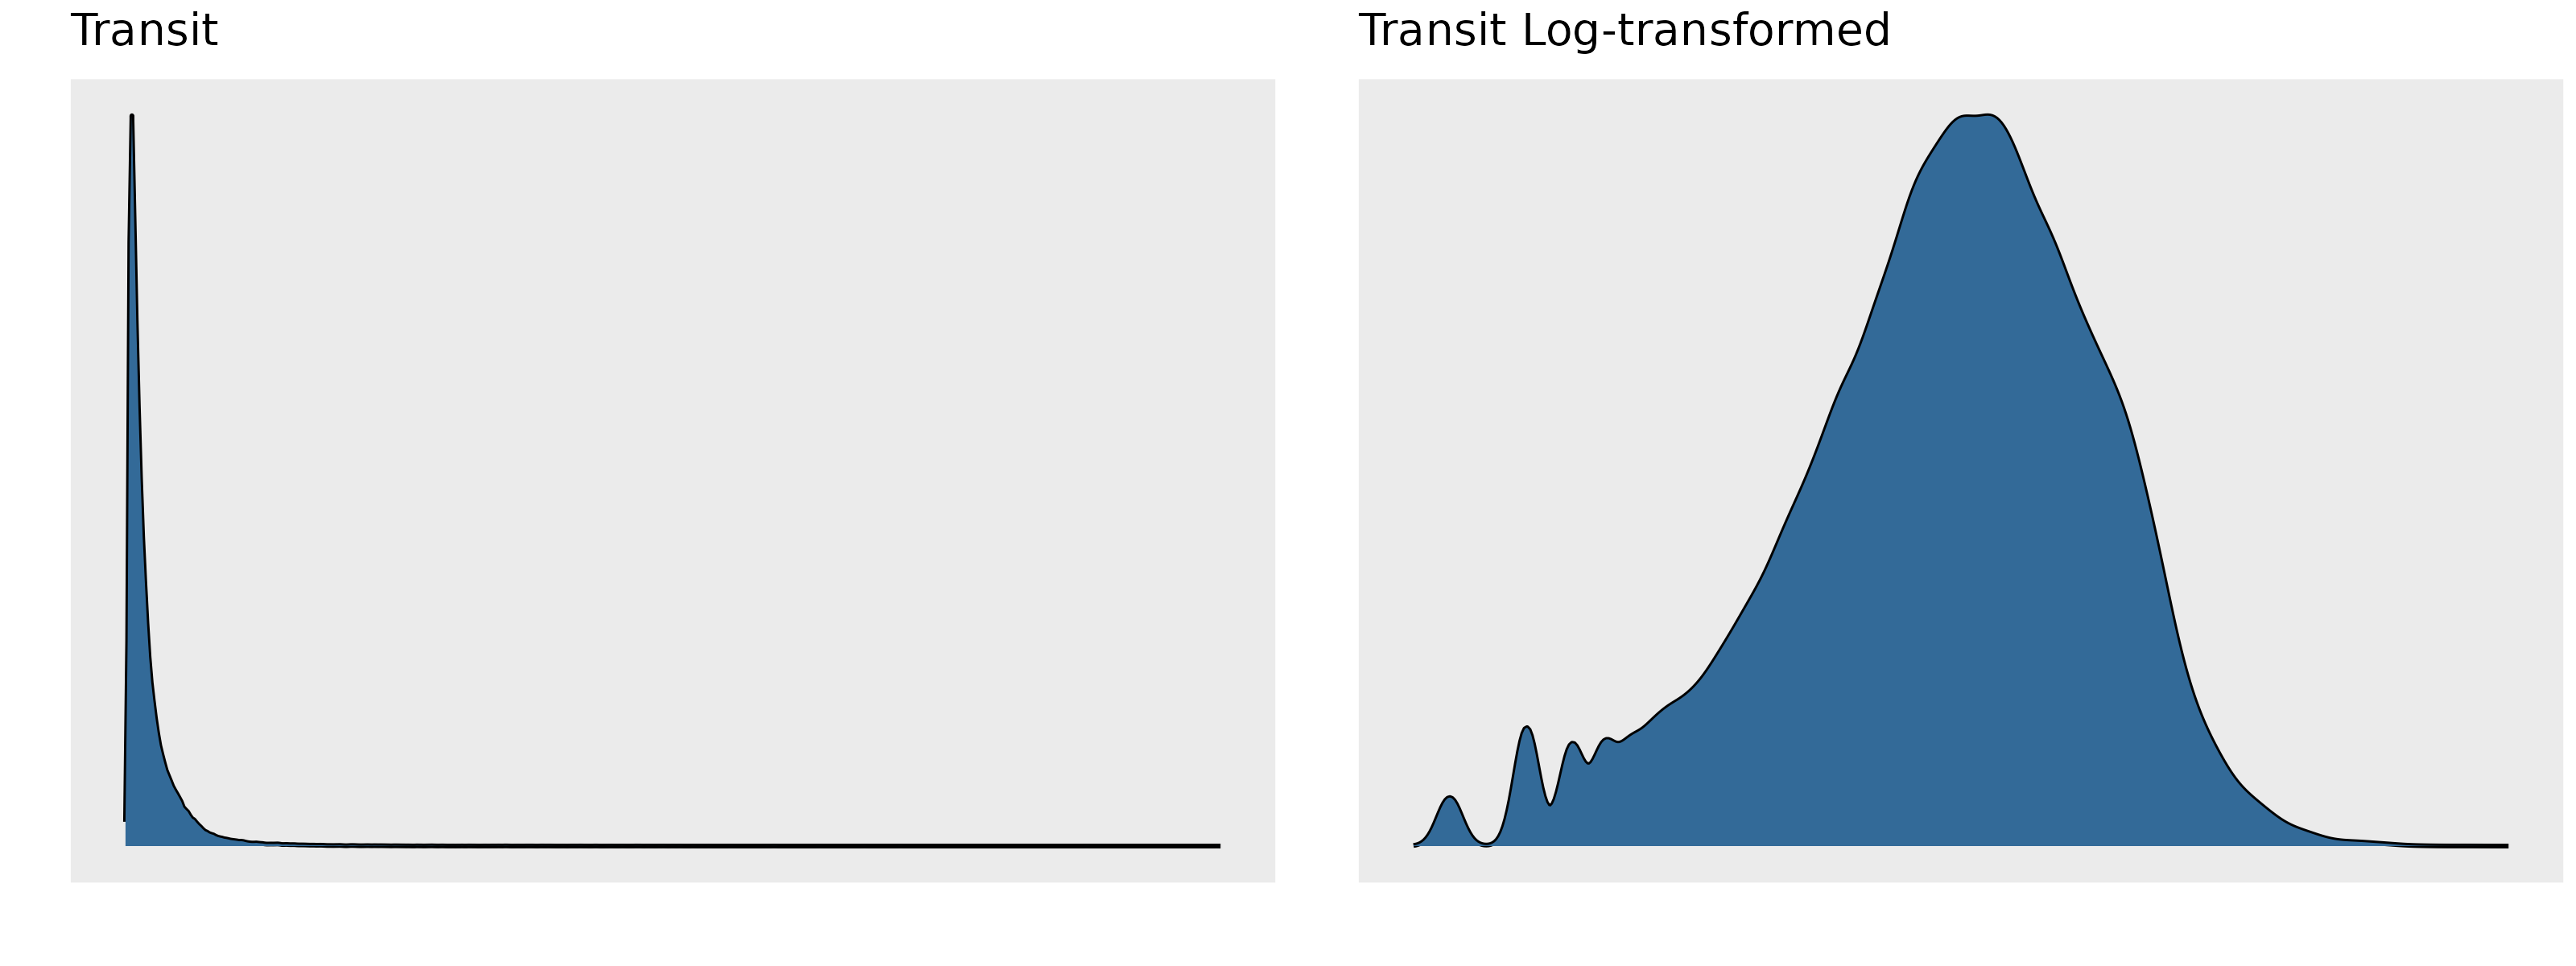
\includegraphics[width=\textwidth]{./distributions/compare_distributions.png}
\caption[Comparison of distributions]{Distribution of the proximity measure to primary education services before and after log-transformation.}\label{comparedist}
\end{figure}






example text Table~\ref{outliercounts} ...


% latex table generated in R 3.6.3 by xtable 1.8-4 package
% Wed May 31 09:55:20 2023
\begin{table}[h]
\centering
\caption[Number of outliers]{The number of outliers in each amenity in the PMD before and after log-transformation.}\label{outliercounts}
\resizebox{\textwidth}{!}{\begin{tabular}{|r|llll|}
  \hline
 & Counts & Percentages & Log Transformed Counts & Log Transformed Percentages \\ 
  \hline
Employment & 45,390 & 9.27 & 0 & 0.00 \\ 
  Pharmacy & 13,416 & 2.74 & 478 & 0.10 \\ 
  Childcare & 15,397 & 3.14 & 140 & 0.03 \\ 
  Healthcare & 31,007 & 6.33 & 50 & 0.01 \\ 
  Grocery & 11,904 & 2.43 & 794 & 0.16 \\ 
  Pri. Educ. & 10,205 & 2.08 & 98 & 0.02 \\ 
  Sec. Educ. & 8,683 & 1.77 & 215 & 0.04 \\ 
  Library & 8,867 & 1.81 & 2,295 & 0.47 \\ 
  Parks & 12,703 & 2.59 & 910 & 0.19 \\ 
  Transit & 14,165 & 2.89 & 3,596 & 0.73 \\ 
   \hline
\end{tabular}}
\end{table}














\subsection{Clustering Tendency}

example text Figure~\ref{prieducvat} ...




\begin{figure}[H]
\centering
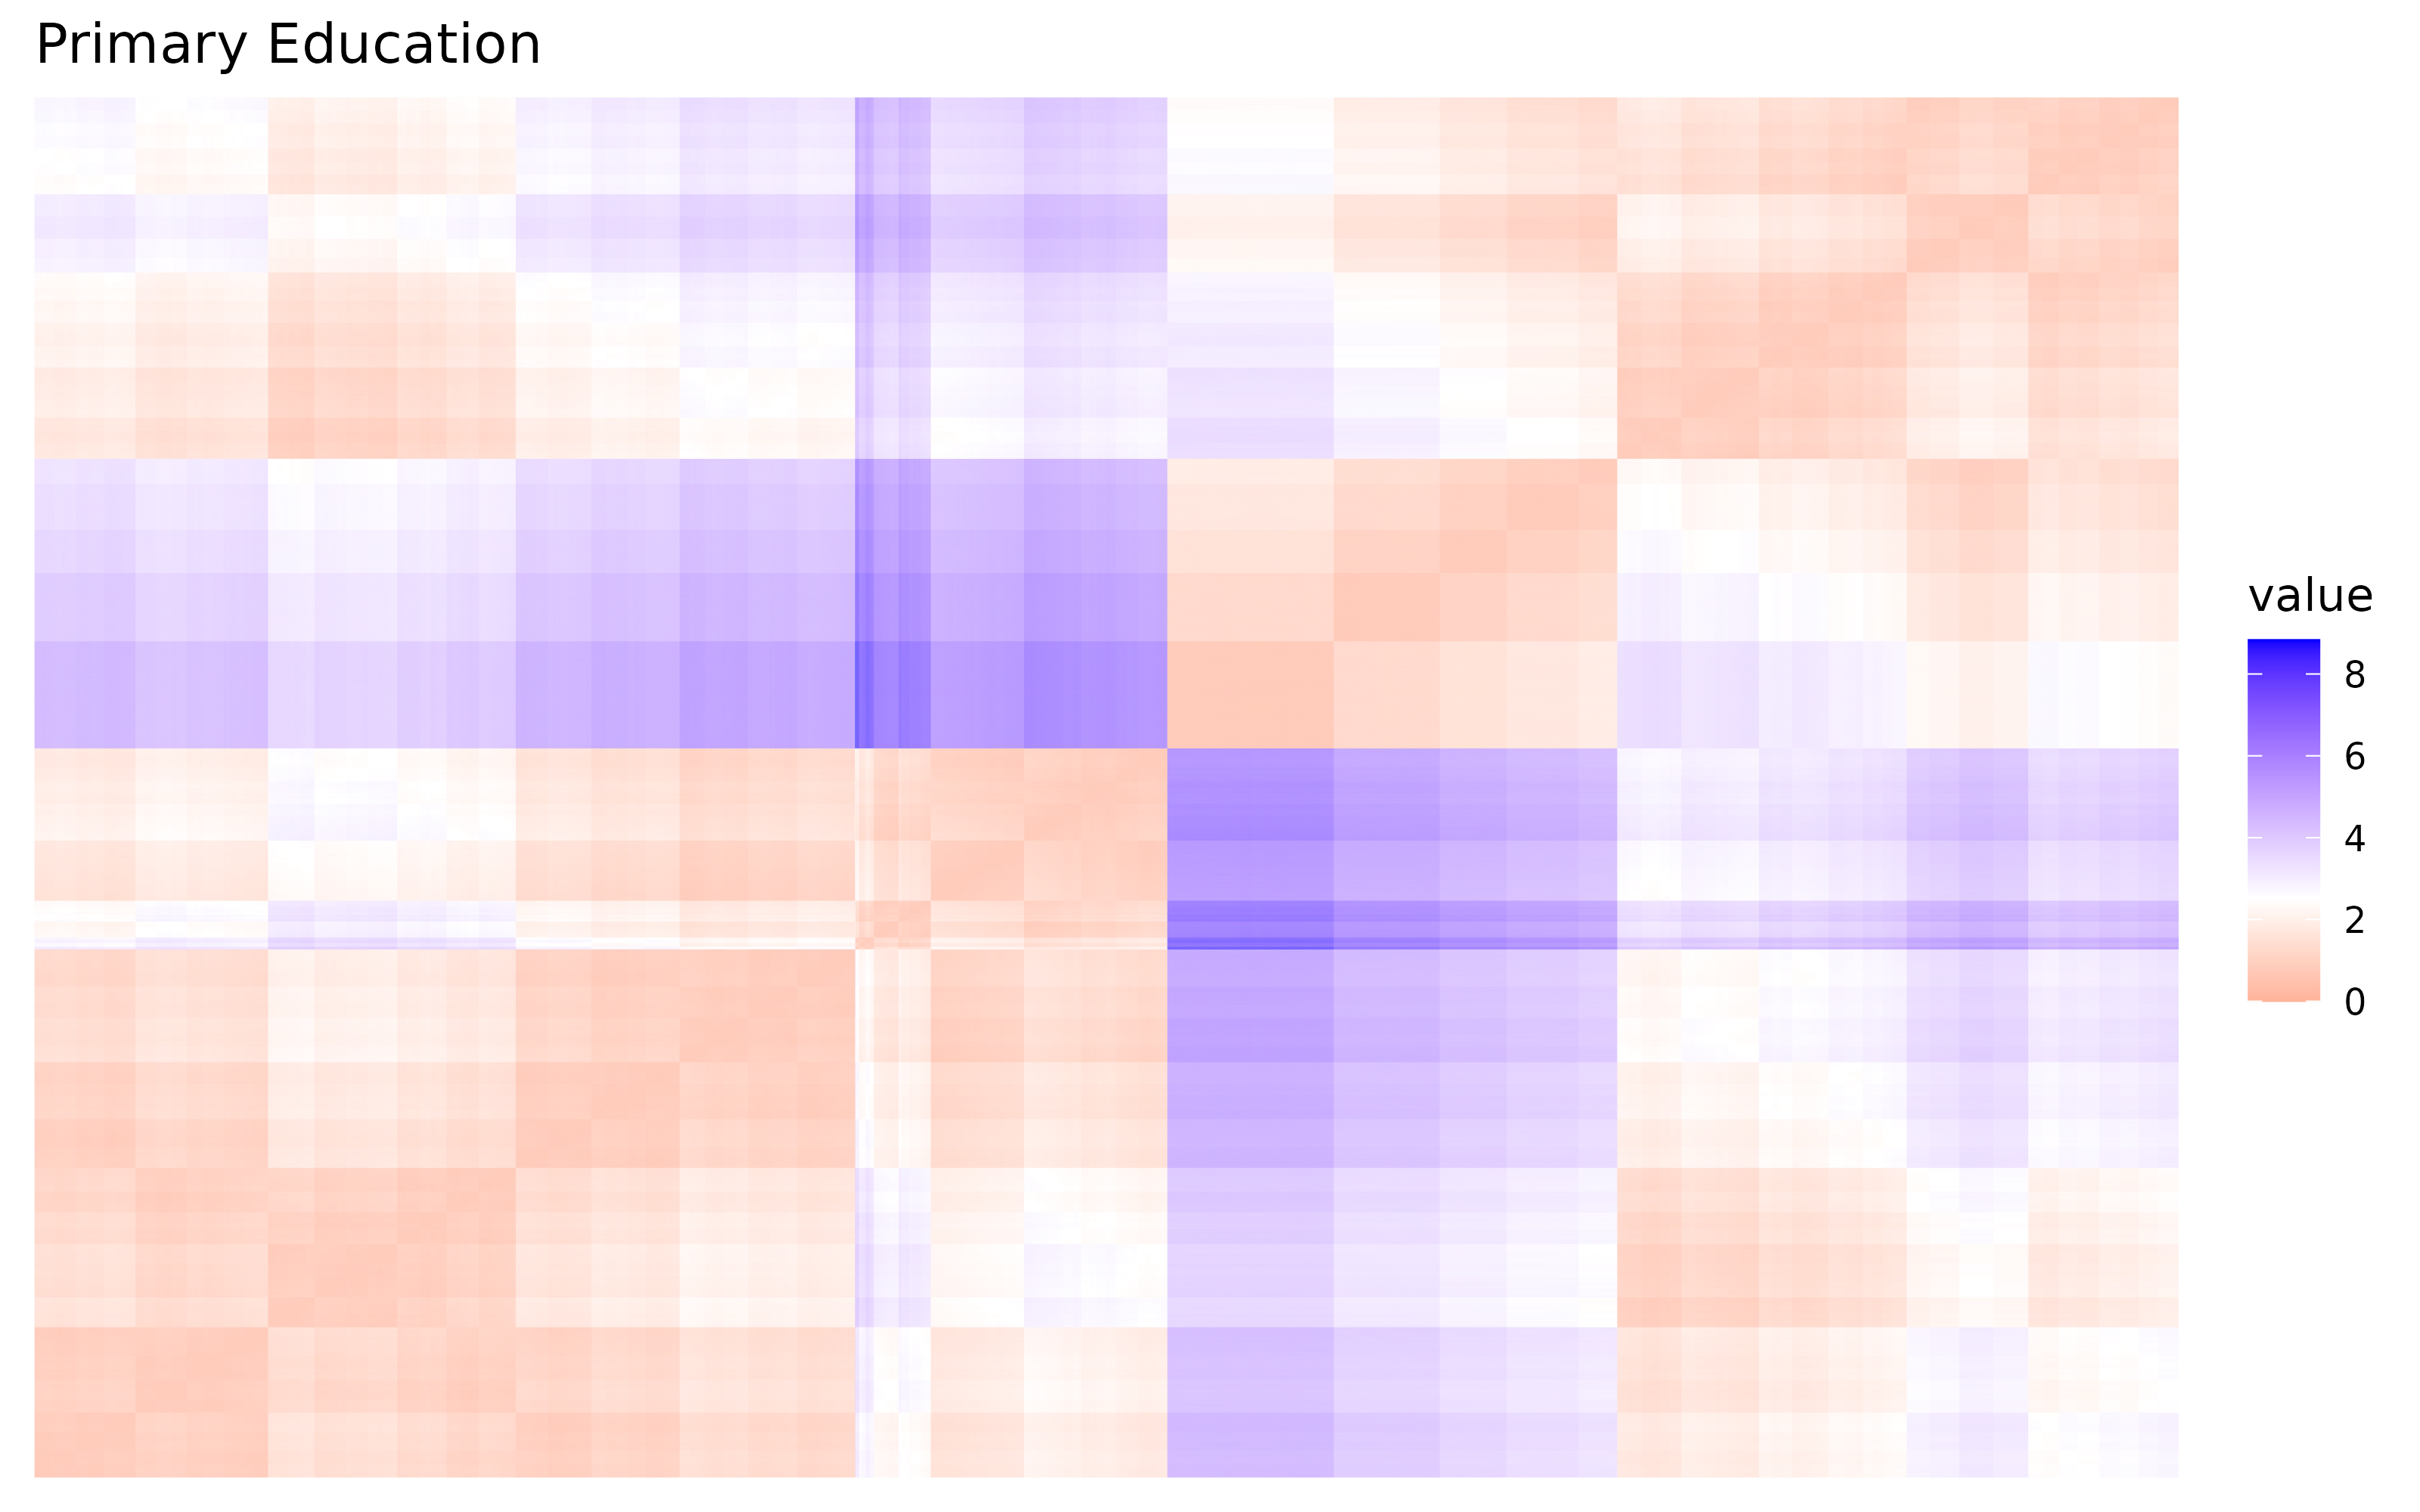
\includegraphics[width=\textwidth]{./vat/primaryeducation_vat_log.png}
\caption[Primary education VAT plot]{VAT plot results for the log-transformed proximity measure of the primary education amenity.}\label{prieducvat}
\end{figure}










example text Figure~\ref{sortplotcompare} ...




\begin{figure}[H]
\centering
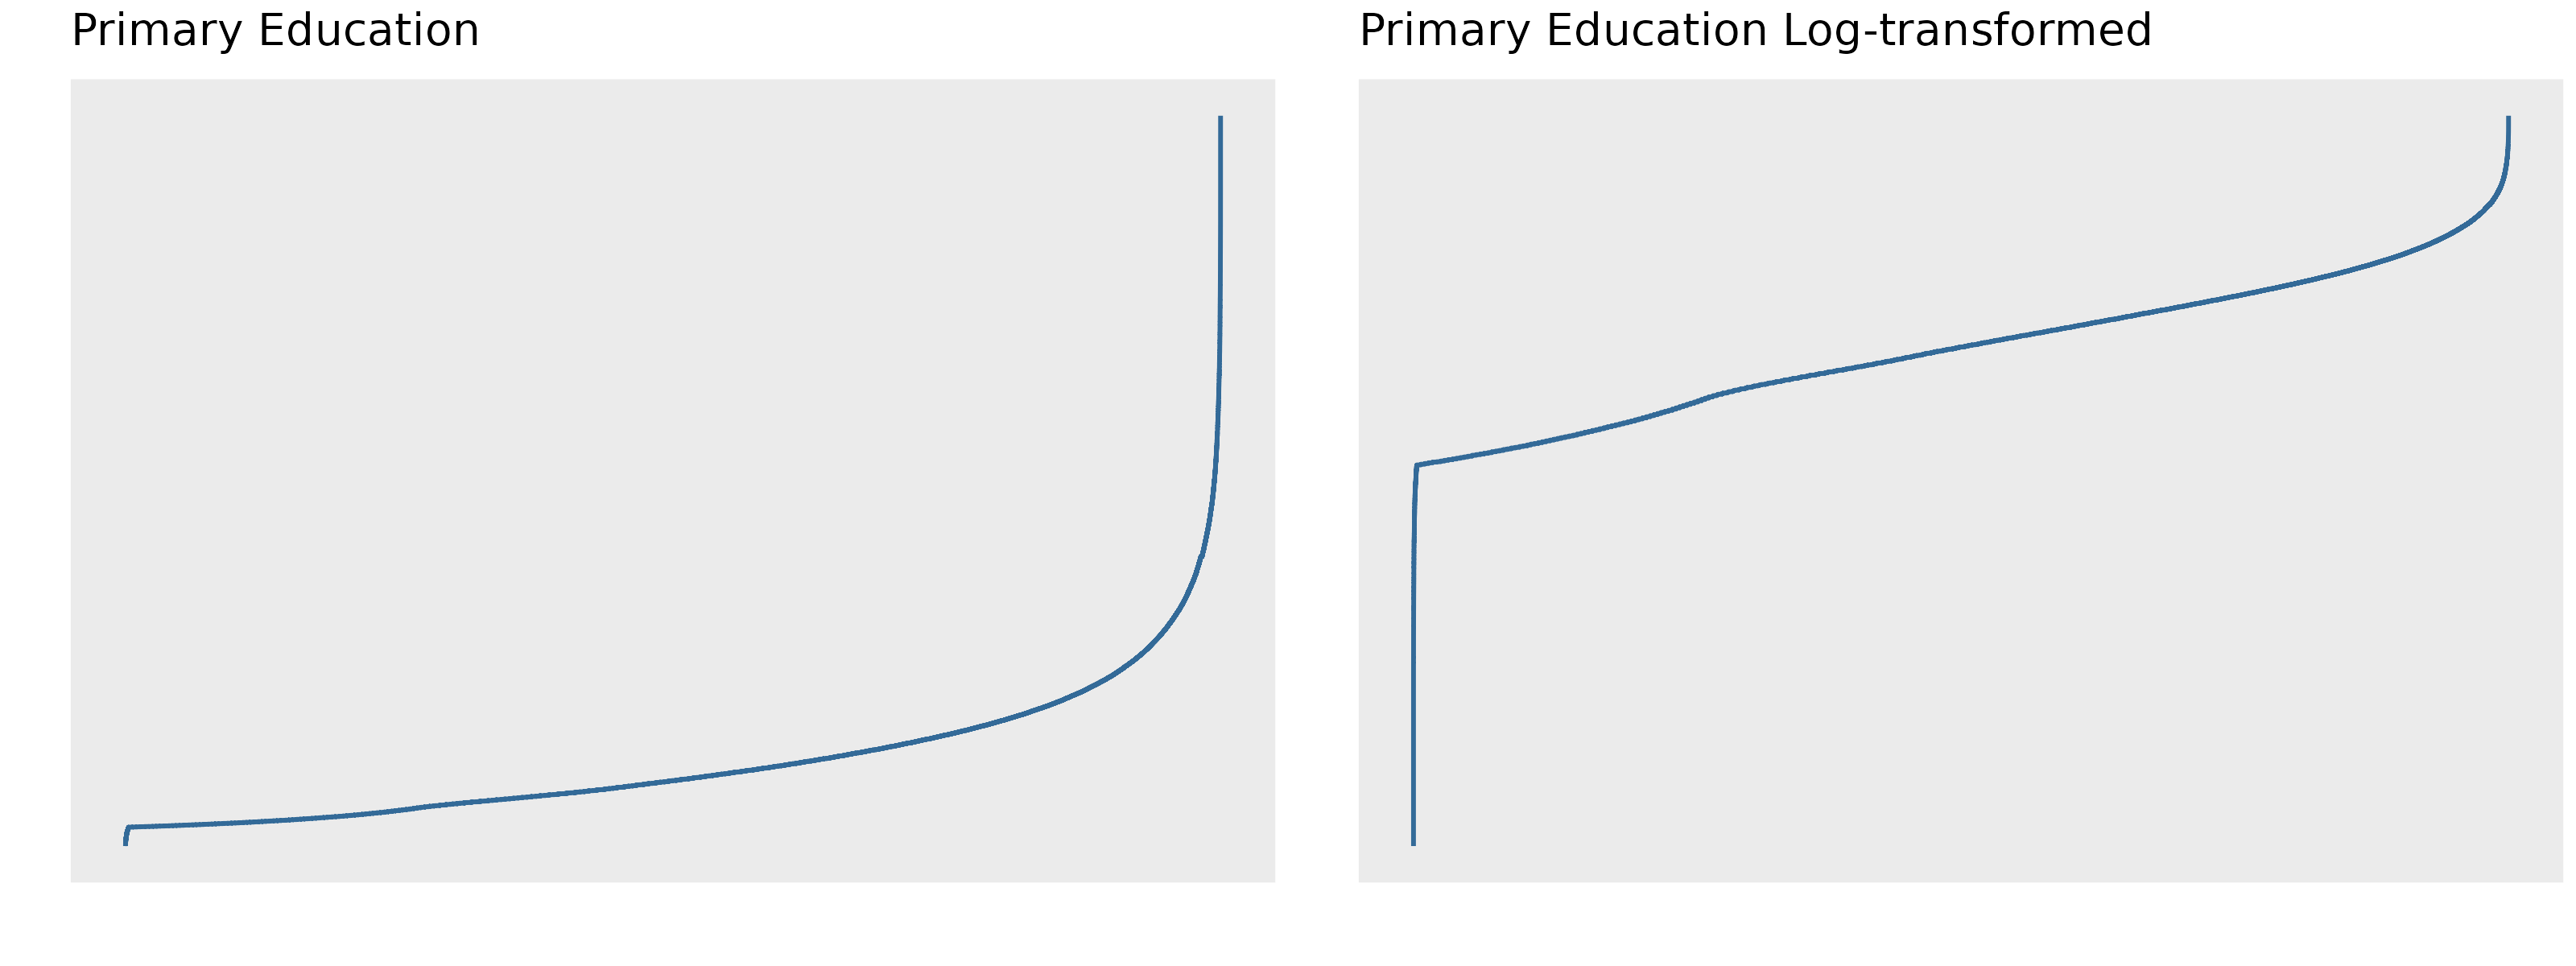
\includegraphics[width=\textwidth]{./sort_plot/sort_comparison.png}
\caption[Primary education sort plot]{Sort plots of the proximity measure to primary education services before and after log-transformation.}\label{sortplotcompare}
\end{figure}








\subsection{Quintiles}













\subsection{Minima Identification}











\subsection{Clustering}


example text Figure~\ref{prieduccutoffs} ...




\begin{figure}[H]
\centering
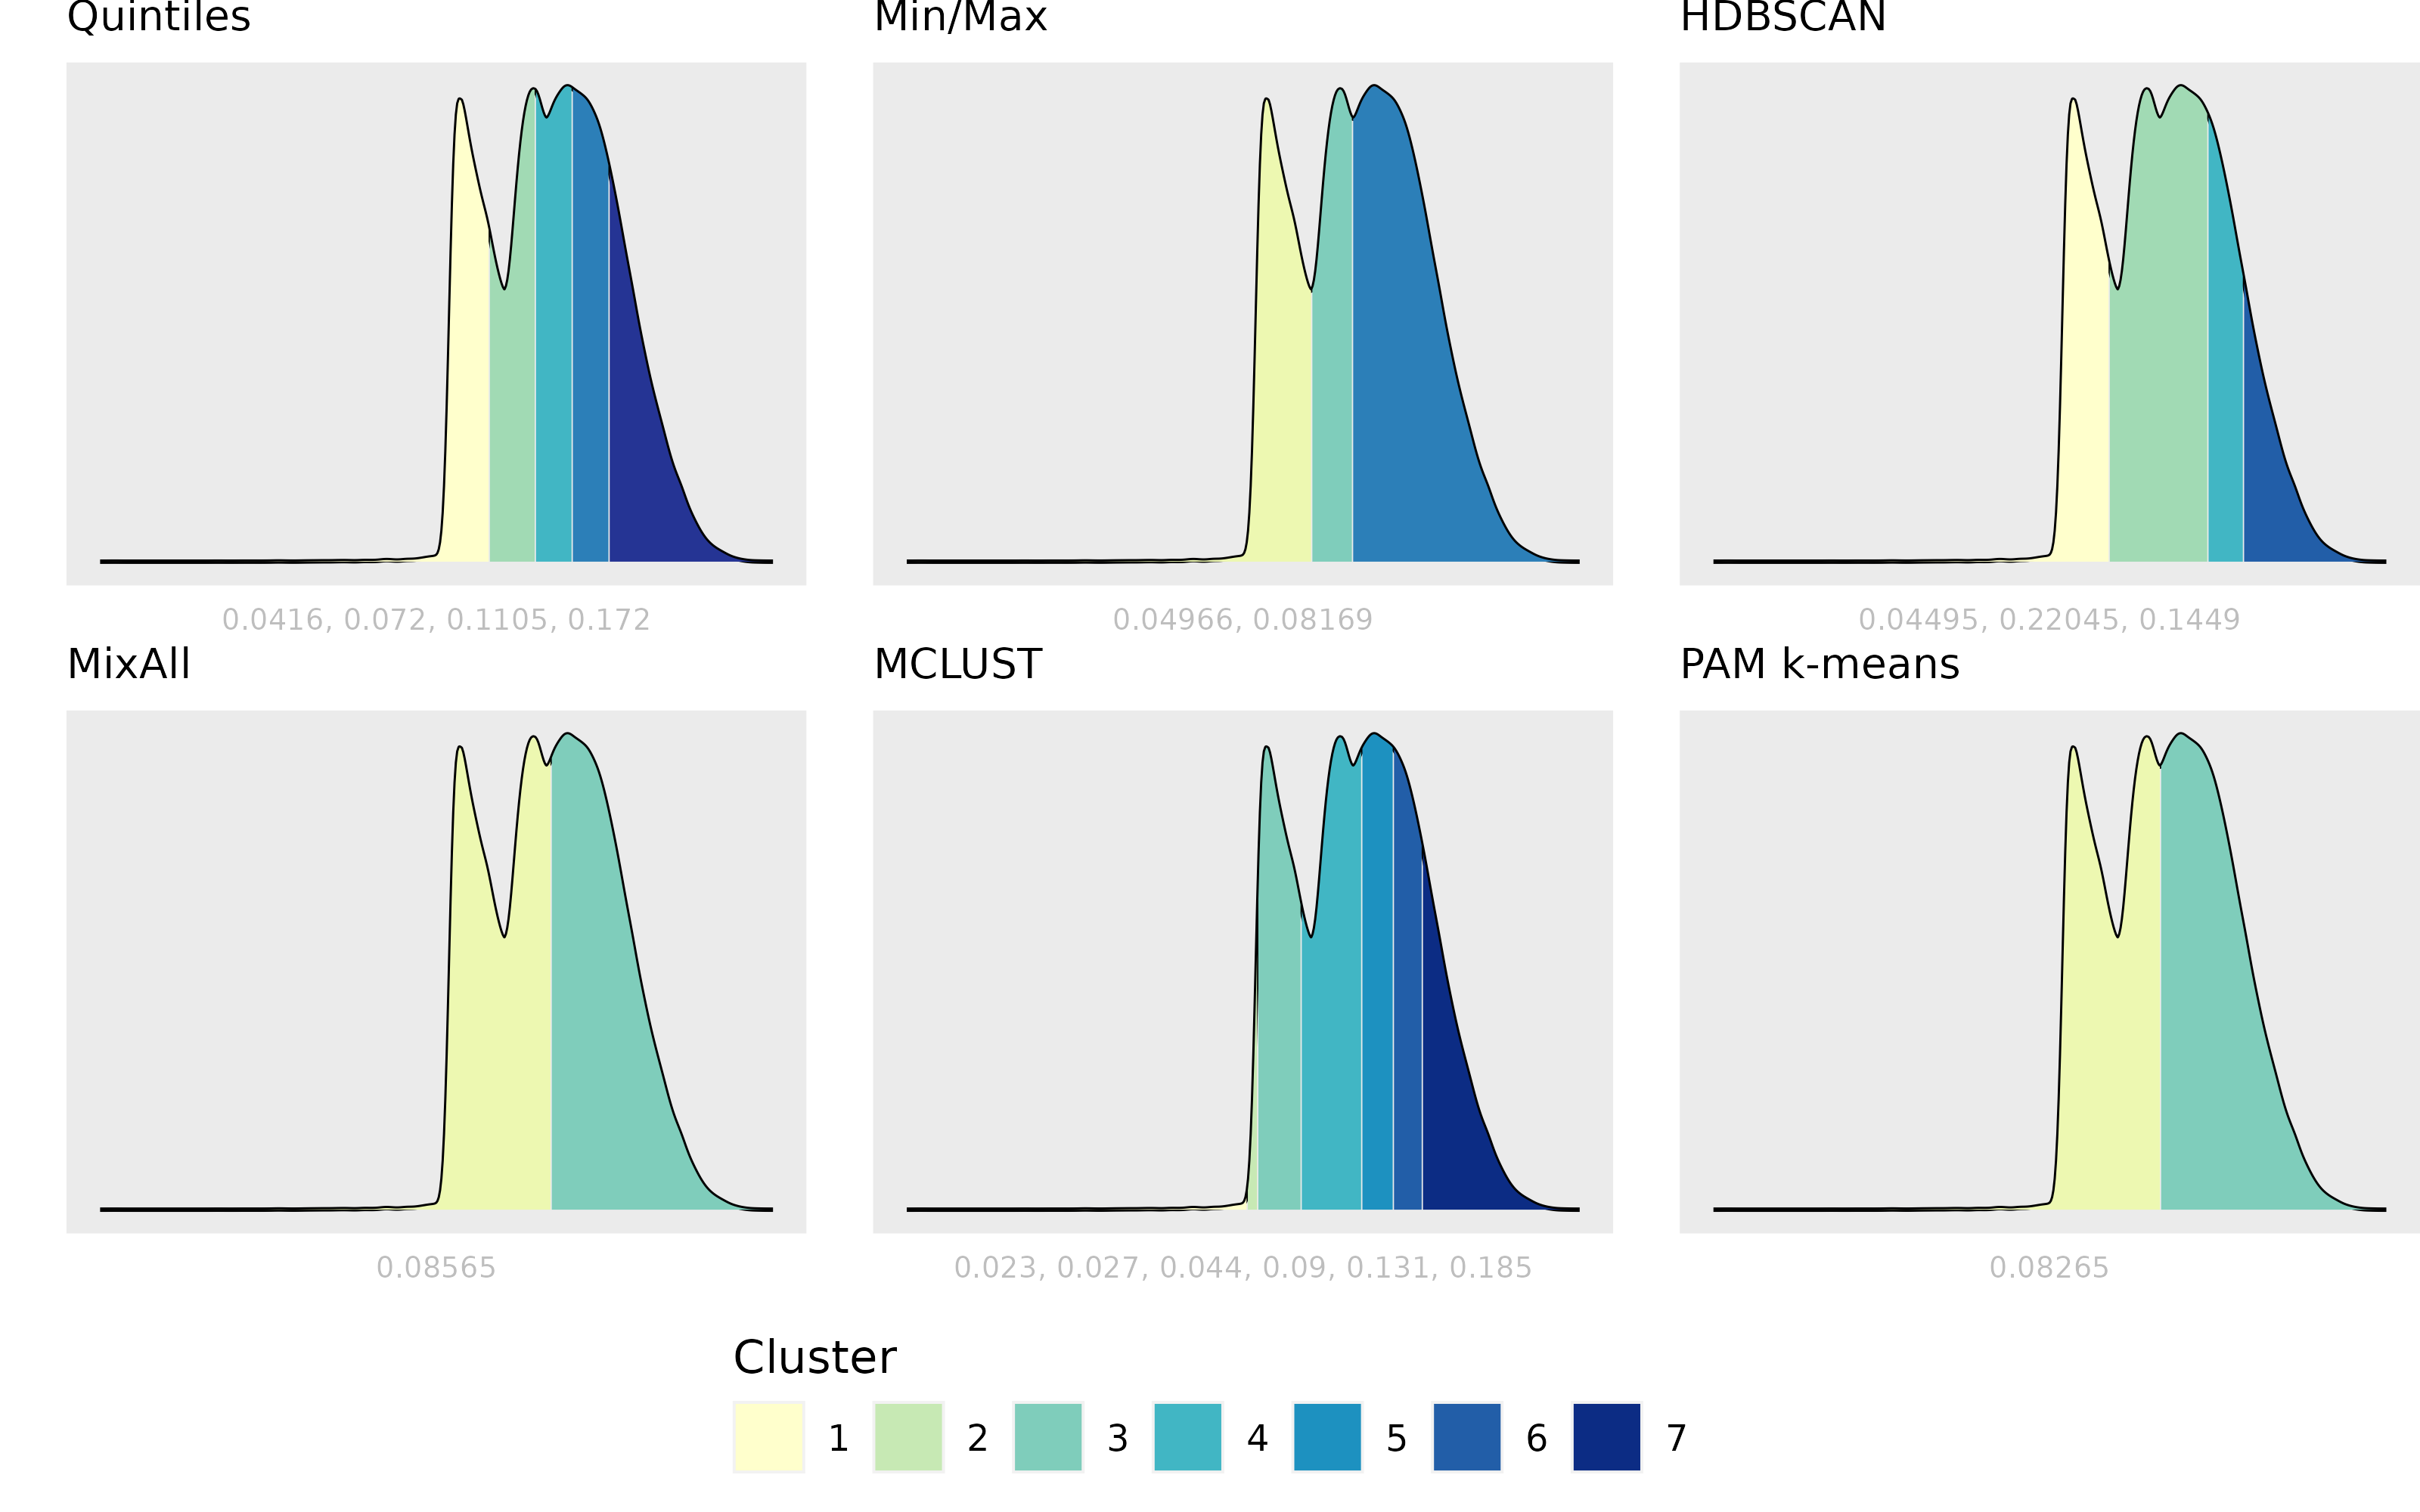
\includegraphics[width=\textwidth]{./cutoffs/by_amenity/Primary Education_cutoffs.png}
\caption[Primary education cutoffs]{Cutoff values from each segmentation approach displayed on the log-transformed density distributions for the primary education amenity.}\label{prieduccutoffs}
\end{figure}






example text Table~\ref{numclusts} ...



% latex table generated in R 3.6.3 by xtable 1.8-4 package
% Fri Jun  9 12:05:37 2023
\begin{table}[ht]
\centering
\caption[Number of clusters by approach]{The number of clusters suggested by all approaches for each amenity in the PMD.}\label{numclusts}
\resizebox{\textwidth}{!}{\begin{tabular}{|r|llllllllll|}
  \hline
 & Emp. & Pharm. & Child. & Health. & Groc. & Pri. Educ. & Sec. Educ. & Lib. & Parks & Transit \\ 
  \hline
Quintiles & 5 & 5 & 5 & 5 & 5 & 5 & 5 & 5 & 5 & 5 \\ 
  Min/Max & 5 & 3 & 3 & 4 & 3 & 3 & 2 & 2 & 3 & 4 \\ 
  HDBSCAN & 2 & 3 & 2 & 2 & 3 & 4 & 3 & 4 & 2 & 2 \\ 
  MixAll & 2 & 2 & 2 & 2 & 2 & 2 & 3 & 2 & 2 & 2 \\ 
  MCLUST & 9 & 7 & 3 & 4 & 3 & 7 & 8 & 7 & 8 & 3 \\ 
  PAM k-means & 2 & 2 & 2 & 2 & 8 & 2 & 4 & 2 & 2 & 2 \\ 
   \hline
\end{tabular}}
\end{table}











example text Table~\ref{prieducmetrics} ...

% latex table generated in R 3.6.3 by xtable 1.8-4 package
% Fri Jun  9 10:09:08 2023
\begin{longtable}{|r|llll|}
  \hline
 & Silhouette & Dunn & Calinski Herzebatz & Davies Bouldin \\ 
  \hline
Quintiles & 0.47 & 0.00000 &  6013 & 0.71 \\ 
   \hline
MixAll & 0.58 & 0.00033 & 15104 & 0.67 \\ 
   \hline
HDBSCAN & 0.33 & 0.00009 &  2594 & 2.69 \\ 
   \hline
PAM k-means & 0.59 & 0.00038 & 15239 & 0.66 \\ 
   \hline
MCLUST & 0.46 & 0.00043 & 18424 & 0.65 \\ 
   \hline
Min/Max & 0.45 & 0.00015 &  2853 & 0.64 \\ 
   \hline
\caption[Primary education validation metrics]{ The validation metric values for each clustering approach for the primary education amenity.}\label{prieducmetrics} 
\end{longtable}












\subsubsection{Cluster Profiles}





example text Table~\ref{prieducprofile} ...


\begin{table}[ht]
\centering
\resizebox{\textwidth}{!}{\begin{tabular}{|r|llllllll|}
  \hline
 & \# of DBs & DB Population & Median IoR & CMA Type & Province & Amenity Dense & Pri. Educ. & Range \\ 
  \hline
Entire Population & 225,359 (100.0\%) & 61 & 0.12 & CMA (65.6\%) & Ontario (24.3\%) & Low (81.3\%) & 0.090 & 0 - 1 \\ 
  Quintiles C1 & 44,802 (19.9\%) & 47 & 0.15 & CMA (53.4\%) & Ontario (17.4\%) & Low (93.1\%) & 0.032 & 0 - 0.0416 \\ 
  Min/Max C1 & 57,009 (25.3\%) & 47 & 0.15 & CMA (52.6\%) & Ontario (17.1\%) & Low (92.9\%) & 0.034 & 0 - 0.0497 \\ 
  HDBSCAN C1 & 50,263 (22.3\%) & 47 & 0.15 & CMA (53.0\%) & Ontario (17.2\%) & Low (93.0\%) & 0.033 & 0 - 0.0449 \\ 
  MixAll C1 & 107,488 (47.7\%) & 50 & 0.14 & CMA (56.1\%) & Ontario (19.1\%) & Low (90.7\%) & 0.047 & 0 - 0.0857 \\ 
  MCLUST C1 & 518 (0.2\%) & 127 & 0.30 & None (72.6\%) & NovaScotia (10.0\%) & Low (100.0\%) & 0.018 & 0 - 0.0235 \\ 
  PAM k-means C1 & 104,320 (46.3\%) & 50 & 0.14 & CMA (55.8\%) & Ontario (19.0\%) & Low (90.8\%) & 0.046 & 0 - 0.0827 \\ 
  Quintiles C2 & 44,830 (19.9\%) & 51 & 0.14 & CMA (56.1\%) & Ontario (19.3\%) & Low (89.8\%) & 0.058 & 0.0416 - 0.0720 \\ 
  Min/Max C2 & 45,865 (20.4\%) & 53 & 0.14 & CMA (59.7\%) & Ontario (21.2\%) & Low (88.4\%) & 0.066 & 0.0497 - 0.0817 \\ 
  HDBSCAN C2 & 113,383 (50.3\%) & 59 & 0.12 & CMA (64.3\%) & Ontario (24.3\%) & Low (84.9\%) & 0.085 & 0.0449 - 0.1449 \\ 
  MixAll C2 & 117,871 (52.3\%) & 69 & 0.11 & CMA (74.3\%) & Ontario (29.0\%) & Low (72.8\%) & 0.149 & 0.0857 - 1 \\ 
  MCLUST C2 & 1,794 (0.8\%) & 48 & 0.15 & CMA (53.2\%) & Ontario (16.6\%) & Low (93.9\%) & 0.026 & 0.0235 - 0.0265 \\ 
  PAM k-means C2 & 121,039 (53.7\%) & 69 & 0.11 & CMA (74.1\%) & Ontario (28.9\%) & Low (73.1\%) & 0.147 & 0.0827 - 1 \\ 
  Quintiles C3 & 45,503 (20.2\%) & 60 & 0.12 & CMA (65.4\%) & Ontario (24.9\%) & Low (84.6\%) & 0.090 & 0.0720 - 0.1105 \\ 
  Min/Max C3 & 122,485 (54.4\%) & 69 & 0.11 & CMA (73.9\%) & Ontario (28.8\%) & Low (73.3\%) & 0.146 & 0.0817 - 1 \\ 
  HDBSCAN C3 & 35,780 (15.9\%) & 70 & 0.11 & CMA (76.4\%) & Ontario (29.9\%) & Low (71.8\%) & 0.174 & 0.1449 - 0.2204 \\ 
  MCLUST C3 & 47,196 (20.9\%) & 46 & 0.15 & CMA (53.4\%) & Ontario (17.4\%) & Low (92.9\%) & 0.033 & 0.0265 - 0.0444 \\ 
  Quintiles C4 & 45,120 (20.0\%) & 67 & 0.11 & CMA (73.7\%) & Ontario (29.9\%) & Low (77.3\%) & 0.137 & 0.1105 - 0.1720 \\ 
  HDBSCAN C4 & 25,933 (11.5\%) & 82 & 0.09 & CMA (80.7\%) & Ontario (30.0\%) & Low (55.9\%) & 0.285 & 0.2204 - 1 \\ 
  MCLUST C4 & 63,570 (28.2\%) & 54 & 0.14 & CMA (59.1\%) & Ontario (20.9\%) & Low (88.3\%) & 0.067 & 0.0444 - 0.0901 \\ 
  Quintiles C5 & 45,104 (20.0\%) & 77 & 0.10 & CMA (79.3\%) & Ontario (29.9\%) & Low (61.9\%) & 0.233 & 0.1720 - 1 \\ 
  MCLUST C5 & 40,185 (17.8\%) & 64 & 0.11 & CMA (70.0\%) & Ontario (28.0\%) & Low (81.5\%) & 0.109 & 0.0901 - 0.1312 \\ 
  MCLUST C6 & 33,300 (14.8\%) & 69 & 0.11 & CMA (75.0\%) & Ontario (29.8\%) & Low (75.0\%) & 0.154 & 0.1312 - 0.1850 \\ 
  MCLUST C7 & 38,796 (17.2\%) & 78 & 0.10 & CMA (79.9\%) & Ontario (30.0\%) & Low (60.1\%) & 0.247 & 0.1850 - 1 \\ 
   \hline
\end{tabular}}
\caption[Primary education cluster profiles]{Summary statistics for each cluster found by all approaches for the primary education amenity. DB Population, IoR and proximity value show the median, while CMA Type, Province and Amenity Dense show the mode.}\label{prieducprofile}
\end{table}










example text Figure~\ref{prieducbarplot} ...




\begin{figure}[H]
\centering
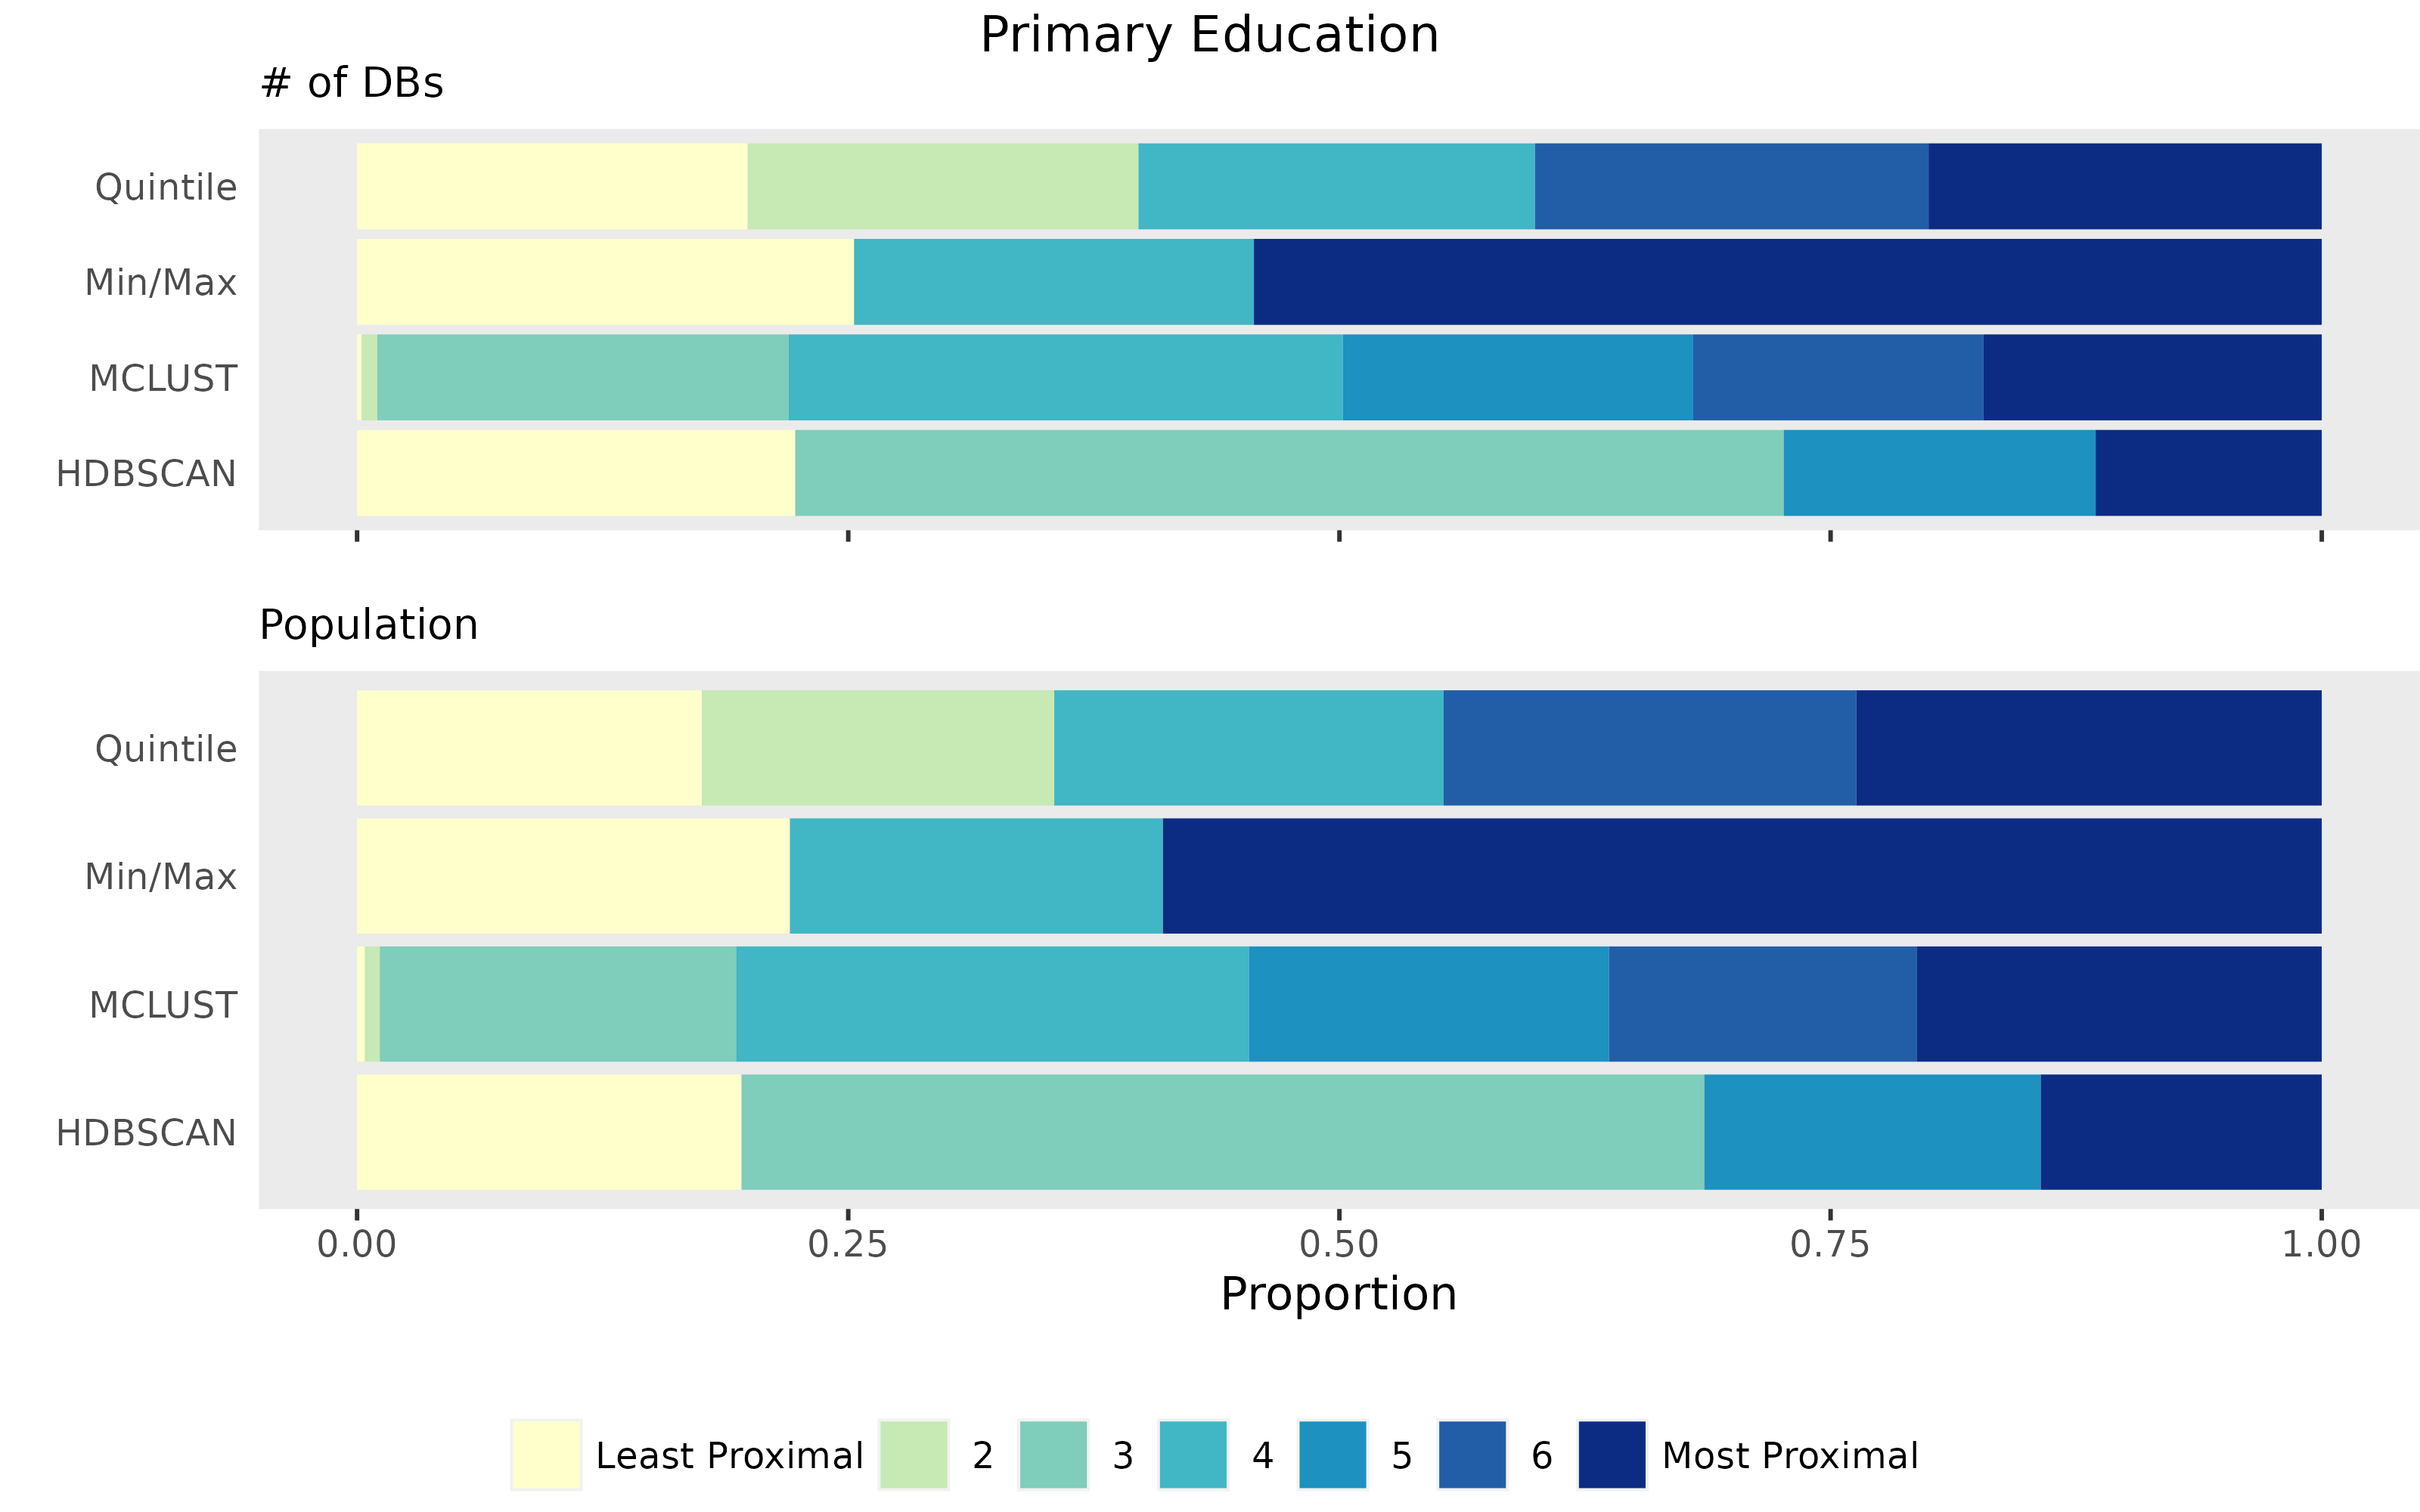
\includegraphics[width=\textwidth]{./barplot_comparison/Primary Education_barplot.png}
\caption[Primary education profile barplot]{Proportion of DBs and population in each cluster for all approaches for the primary education amenity.}\label{prieducbarplot}
\end{figure}










\pagebreak 
%%%%%%%%%%%%%%%%%%%%%%%%%%%%%%%%%%%%%%%%
\section{Discussion}
%%%%%%%%%%%%%%%%%%%%%%%%%%%%%%%%%%%%%%%%




text 







\subsection{Comparison of Approaches}


















\subsection{Interpretation of Cluster Profiles}
























\pagebreak 
%%%%%%%%%%%%%%%%%%%%%%%%%%%%%%%%%%%%%%%%
\section{Limitations}
%%%%%%%%%%%%%%%%%%%%%%%%%%%%%%%%%%%%%%%%

























\pagebreak 
%%%%%%%%%%%%%%%%%%%%%%%%%%%%%%%%%%%%%%%%
\section{Conclusion}
%%%%%%%%%%%%%%%%%%%%%%%%%%%%%%%%%%%%%%%%


















\pagebreak
\section{References}


\bibliographystyle{apa}
\renewcommand{\bibsection}{}
\bibliography{final_sources.bib}



\pagebreak
\appendix
\section{Appendix}
\par
text





\subsection{Successful Methods}











\subsection{Unsuccessful Methods}

\subsubsection{Univariate Clustering}









\subsubsection{Multivariate Clustering}










\subsection{Extra Plots and Tables}






\begin{table}[H]
\centering
\resizebox{\textwidth}{!}{
\begin{tabularx}{\textwidth}{|p{2cm}|X|} 
\hline
\textbf{Amenity} & \textbf{Definition} \\
\hline
\textit{Employment} & Measures the closeness of a dissemination block to any dissemination block with a source of employment within a driving distance of 10 km. This measure is derived from the employment counts of all businesses -- that is, all North American Industry Classification (NAICS) codes in the Business Register. \\ 
\hline 
\textit{Grocery} & Measures the closeness of a dissemination block to any dissemination block with a grocery store within a walking distance of 1 km. This measure is derived from the total revenue of all NAICS 4451 businesses in the Business Register. \\ 
\hline 
\textit{Pharmacy} & Measures the closeness of a dissemination block to any dissemination block with a pharmacy or a drug store within a walking distance of 1 km. This measure is derived from the presence of all NAICS 446110 businesses in the Business Register. \\ 
\hline 
\textit{Health care} & Measures the closeness of a dissemination block to any dissemination block with a health care facility within a driving distance of 3 km. This measure is derived from the employment counts of all NAICS 6211, 6212, 6213, 621494, and 622 businesses in the Business Register. \\ 
\hline 
\textit{Child care} & Measures the closeness of a dissemination block to any dissemination block with a child care facility within a walking distance of 1.5 km. This measure is derived from the presence of all NAICS 624410 businesses in the Business Register. \\ 
\hline 
\textit{Primary} \newline \textit{Education} & Measures the proximity to primary education measures the closeness of a dissemination block to any dissemination block with a primary school within a walking distance of 1.5 km. Primary schools are classified as education facilities with an International Standard Classification of education (ISCED) level of 1. The data source is a conglomeration of the Open Database of Education Facilities and other sources of education facilities. \\ 
\hline 
\textit{Secondary} \newline \textit{Education} & Measures the closeness of a dissemination block to any dissemination block with a secondary school within a walking distance of 1.5 km. The data source is a conglomeration of the Open Database of Education Facilities and other sources of education facilities where secondary schools are classified as ISCED2 and/or ISCED3. \\ 
\hline 
\textit{Transit} & Measures the closeness of a dissemination block to any source of public transportation within a 1 km walking distance. This measure is derived from the number of all trips between 7:00 a.m. - 10:00 a.m. from a conglomeration of General Transit Feed Specification (GTFS) data sources. \\ 
\hline 
\textit{Parks} & Measures the closeness of a dissemination block to any dissemination block with a neighborhood park within a 1 km walking distance. This measure is derived from the presence of all parks from a conglomeration of authoritative open data sources and OpenStreetMap. \\ 
\hline 
\textit{Libraries} & Measures the closeness of a dissemination block to any dissemination block with a library within a 1.5 km walking distance. This measure is derived from the presence of all libraries from a conglomeration of open and publicly available data sources. \\ 
\hline 
\textit{Amenity Dense} & An aggregate measure was created to indicate neighbourhoods that have access to basic needs for a family with minors. A dissemination block with access to a grocery store, pharmacy, health care facility, child care facility, primary school, library, public transit stop, and source of employment is referred to as an amenity dense neighbourhood. A high amenity density neighbourhood is defined as an amenity dense neighbourhood that has proximity measure values in the top third of the distribution for each of the eight proximity measures. \\ 
\hline 
\hline
\end{tabularx}
}
\caption[Data dictionary]{Data Dictionary for the PMD.}\label{datadictionary}
\end{table}







\begin{table}[H]
\centering
\resizebox{\textwidth}{!}{
\begin{tabular}{|r|llllllllll|}
  \hline
 & Employment & Pharmacy & Childcare & Healthcare & Grocery & Pri. Educ. & Sec. Educ. & Library & Parks & Transit \\ 
  \hline
1 Dec. & -8.51719 & -4.87961 & -4.82831 & -8.11173 & -4.23361 & -3.44202 & -3.28341 & -2.97789 & -4.35831 & -6.72543 \\ 
  2 Dec. & -7.6009 & -4.61522 & -4.1799 & -7.1309 & -3.80766 & -3.17725 & -3.16534 & -2.88419 & -3.89222 & -5.9145 \\ 
  3 Dec. & -6.57128 & -4.21991 & -3.7214 & -6.2659 & -3.54046 & -2.84215 & -3.02413 & -2.77259 & -3.57913 & -5.3817 \\ 
  4 Dec. & -5.77635 & -3.94248 & -3.35527 & -5.71383 & -3.35527 & -2.6297 & -2.83532 & -2.6479 & -3.28876 & -4.99083 \\ 
  5 Dec. & -5.02069 & -3.66126 & -3.04282 & -5.27851 & -3.13499 & -2.40684 & -2.59561 & -2.50715 & -3.0324 & -4.65646 \\ 
  6 Dec. & -4.35831 & -3.37553 & -2.75357 & -4.89285 & -2.88957 & -2.20184 & -2.3958 & -2.34237 & -2.78872 & -4.32754 \\ 
  7 Dec. & -3.82585 & -3.08347 & -2.46864 & -4.49184 & -2.63109 & -1.98997 & -2.1698 & -2.14644 & -2.53326 & -3.98998 \\ 
  8 Dec. & -3.29954 & -2.74575 & -2.14729 & -3.98998 & -2.31668 & -1.75968 & -1.9018 & -1.90448 & -2.25284 & -3.60087 \\ 
  9 Dec. & -2.62141 & -2.31871 & -1.74183 & -3.3697 & -1.87015 & -1.45629 & -1.54693 & -1.55732 & -1.90046 & -3.11677 \\ 
  Min. & -9.21034 & -9.21034 & -9.21034 & -9.21034 & -8.517193 & -7.600902 & -7.418581 & -8.517193 & -9.21034 & -9.21034 \\ 
  Median & -5.02069 & -3.66126 & -3.04282 & -5.27851 & -3.13499 & -2.40684 & -2.59561 & -2.50715 & -3.0324 & -4.65646 \\ 
  Mean & -5.30642 & -3.60872 & -3.14453 & -5.50353 & -3.08437 & -2.41781 & -2.51013 & -2.36977 & -3.06704 & -4.80398 \\ 
  Max. & 1e-04 & 1e-04 & 1e-04 & 1e-04 & 1e-04 & 1e-04 & 1e-04 & 1e-04 & 1e-04 & 1e-04 \\ 
  Std. Dev. & 2.1556 & 0.9607 & 1.1298 & 1.7612 & 0.9114 & 0.7301 & 0.668 & 0.5789 & 0.9174 & 1.4123 \\ 
  Skew & -0.237 & 0.363 & -0.208 & -0.344 & 0.132 & 0.112 & 0.605 & 1.024 & -0.154 & -0.55 \\ 
  Kurtosis & 2 & 2.54 & 2.43 & 2.53 & 2.85 & 2.32 & 2.63 & 4.14 & 3.04 & 3.21 \\ 
   \hline
\end{tabular}
}
\caption[Log summary table]{Summary statistics of log-transformed numerical variables from the PMD.}\label{logsummary}
\end{table}








\pagebreak

\begin{figure}[H]
\centering
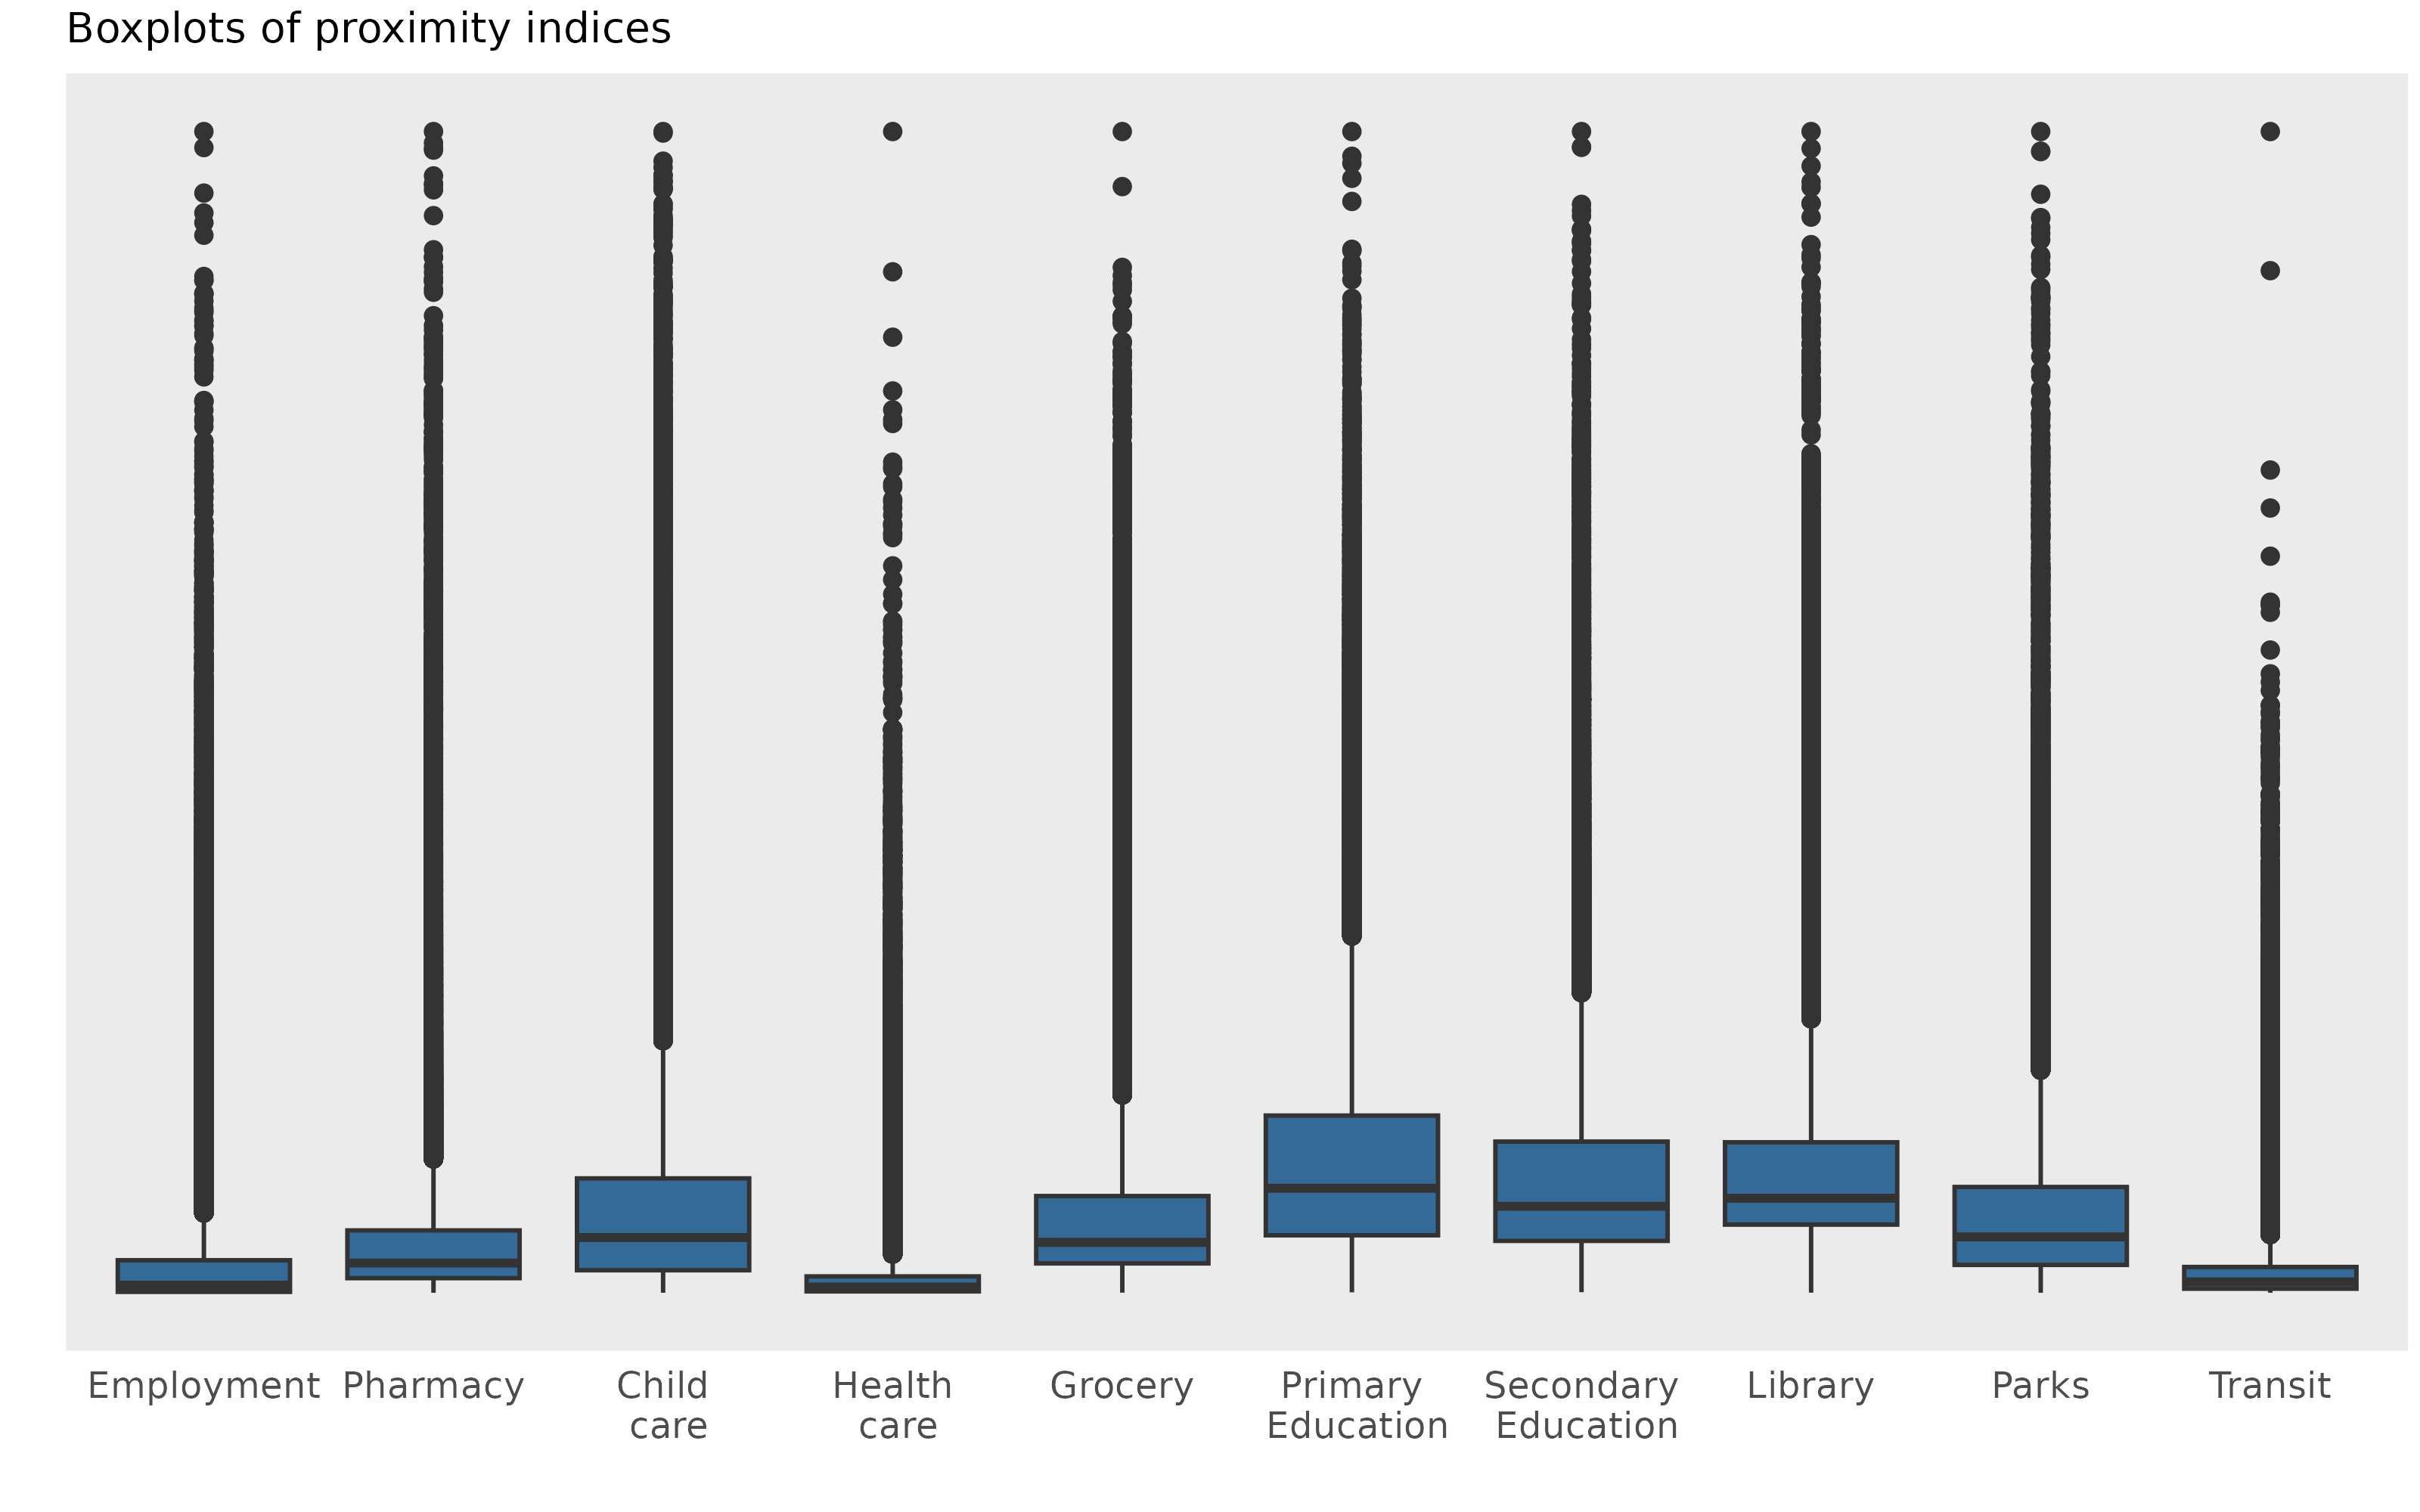
\includegraphics[width=\textwidth]{./outliers/boxplot.png}
\caption[Boxplots of outliers]{Boxplots showing outliers for all ten amenities of the PMD.}\label{boxoutliers}
\end{figure}







\begin{figure}[H]
\centering
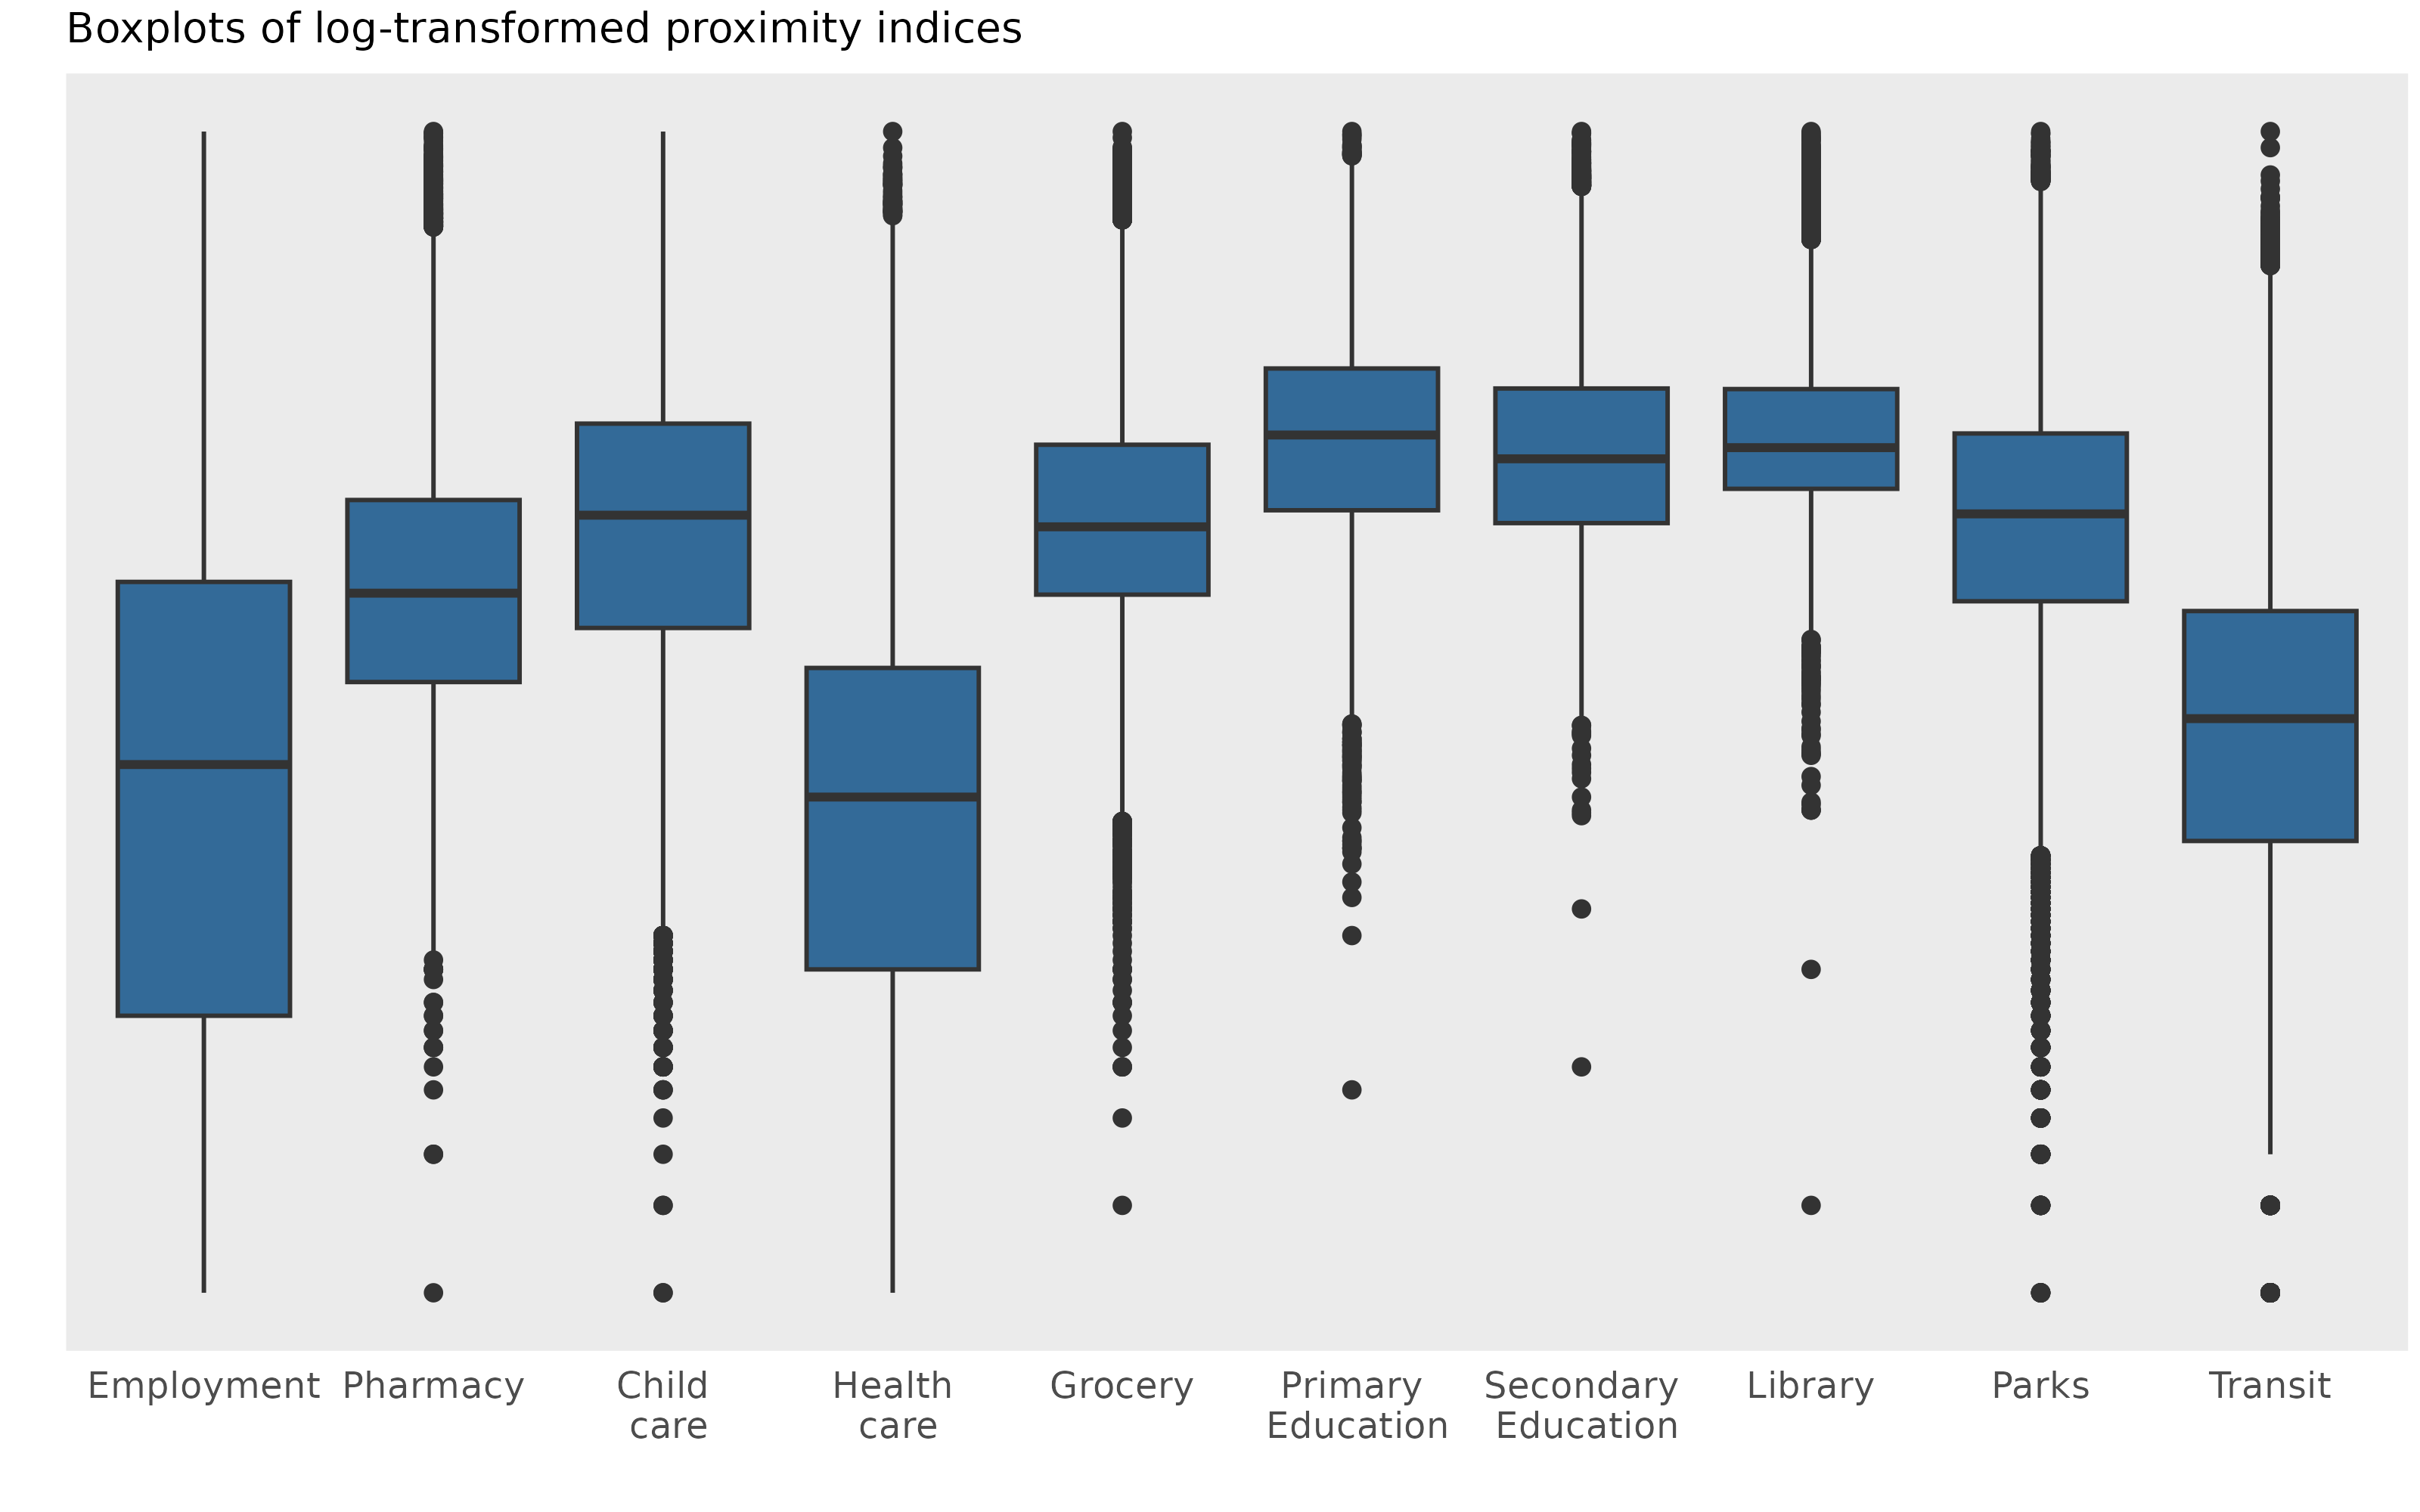
\includegraphics[width=\textwidth]{./outliers/logged_boxplot.png}
\caption[Boxplots of log outliers]{ Boxplots showing outliers for all ten log-transformed amenities of the PMD.}\label{logboxoutliers}
\end{figure}







\begin{figure}[H]
\centering
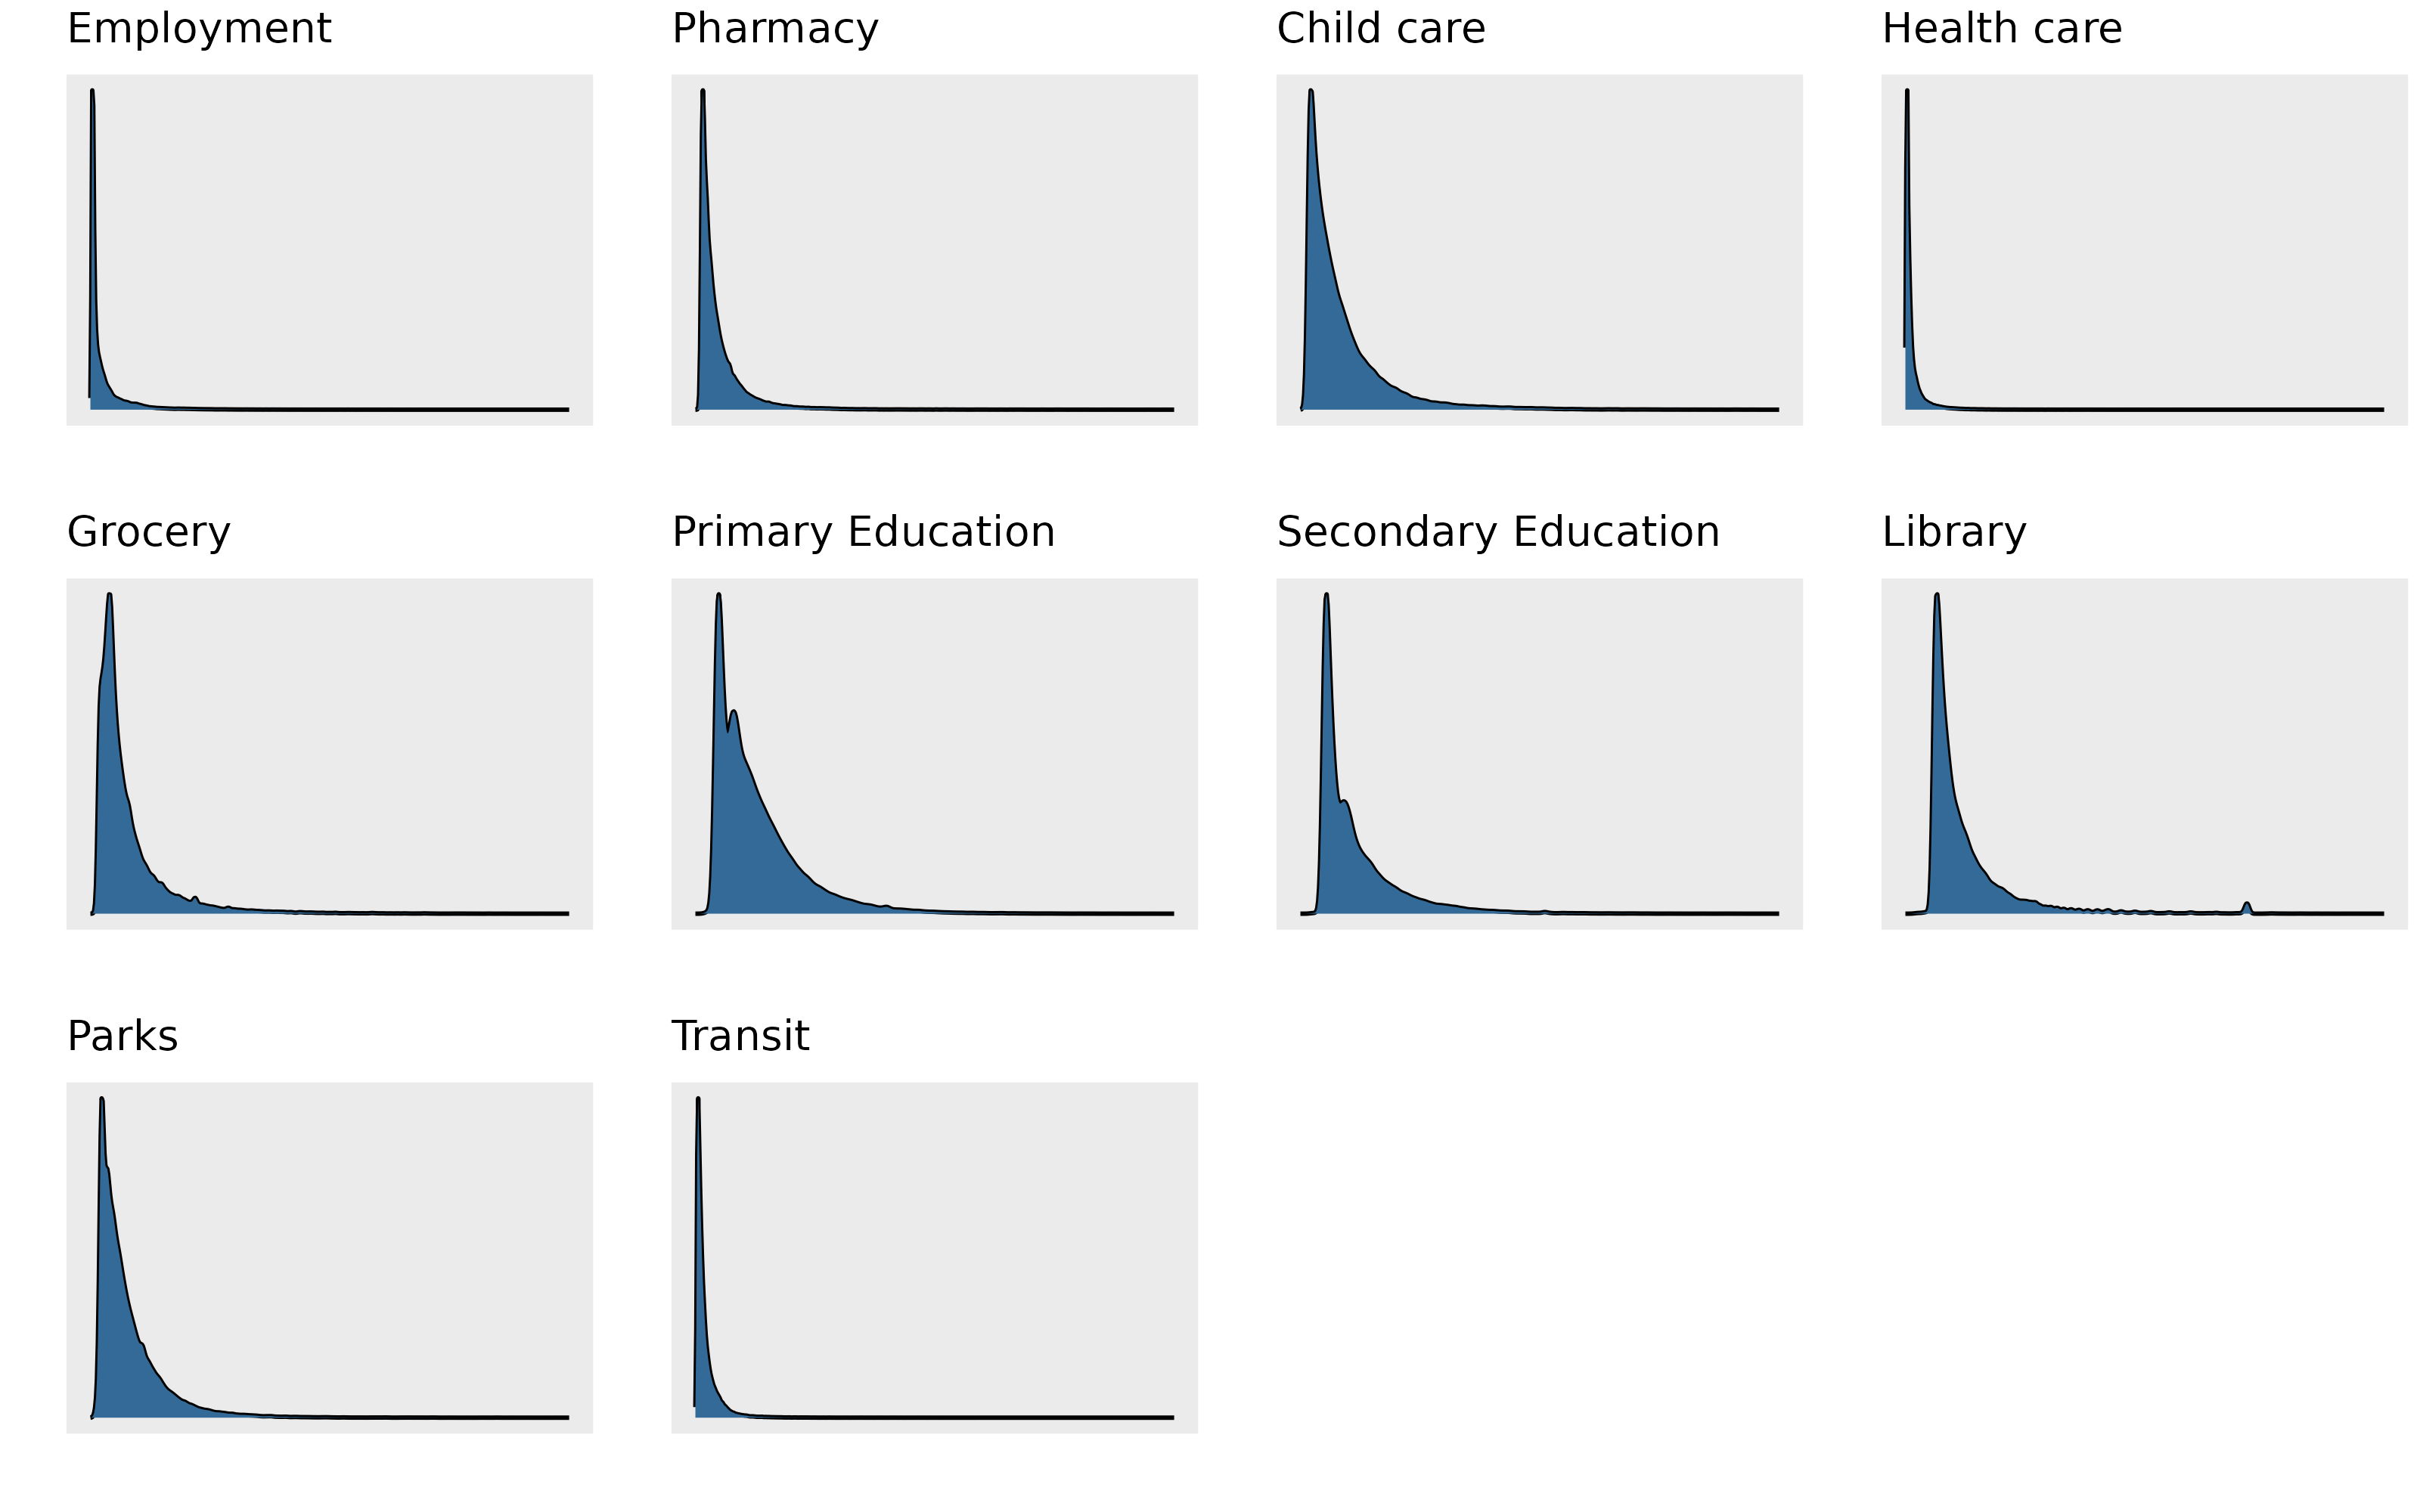
\includegraphics[width=\textwidth]{./distributions/distributions.png}
\caption[Density distributions]{Density distributions for all ten amenities of the PMD.}\label{dendist}
\end{figure}







\begin{figure}[H]
\centering
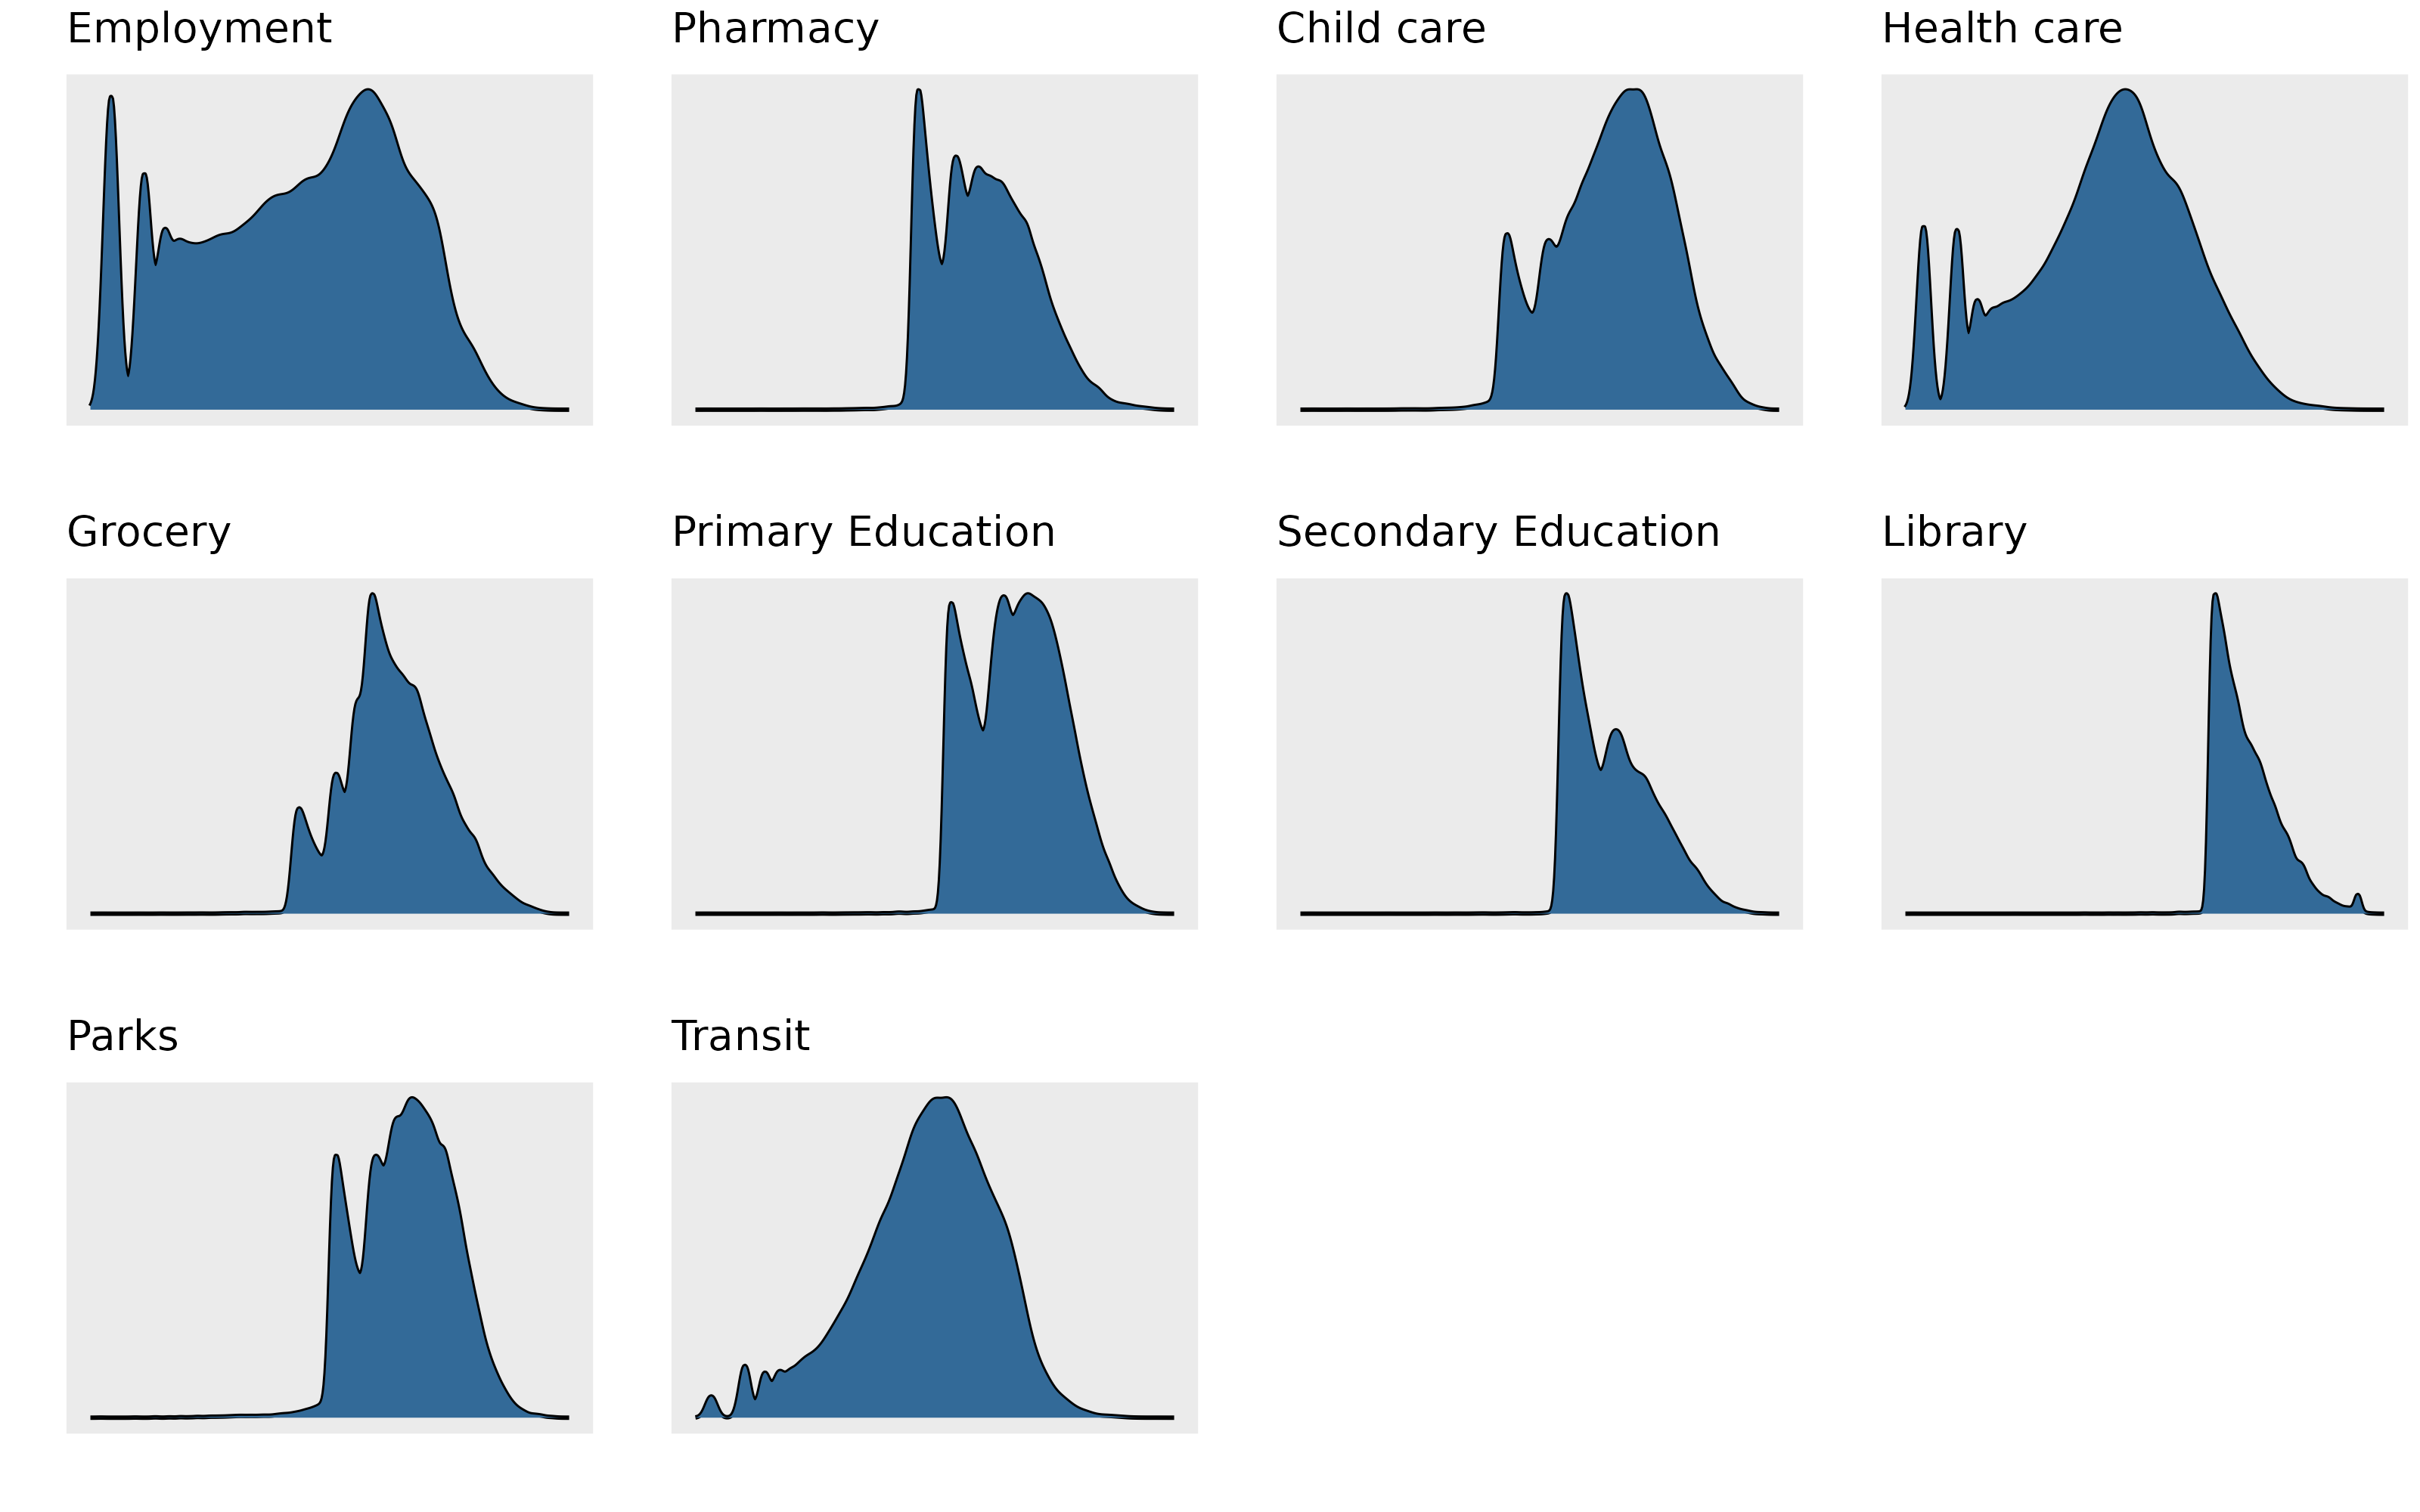
\includegraphics[width=\textwidth]{./distributions/log_distributions.png}
\caption[Log density distributions]{ Log-transformed density distributions for all ten amenities of the PMD.}\label{logdendist}
\end{figure}







\begin{figure}[H]
\centering
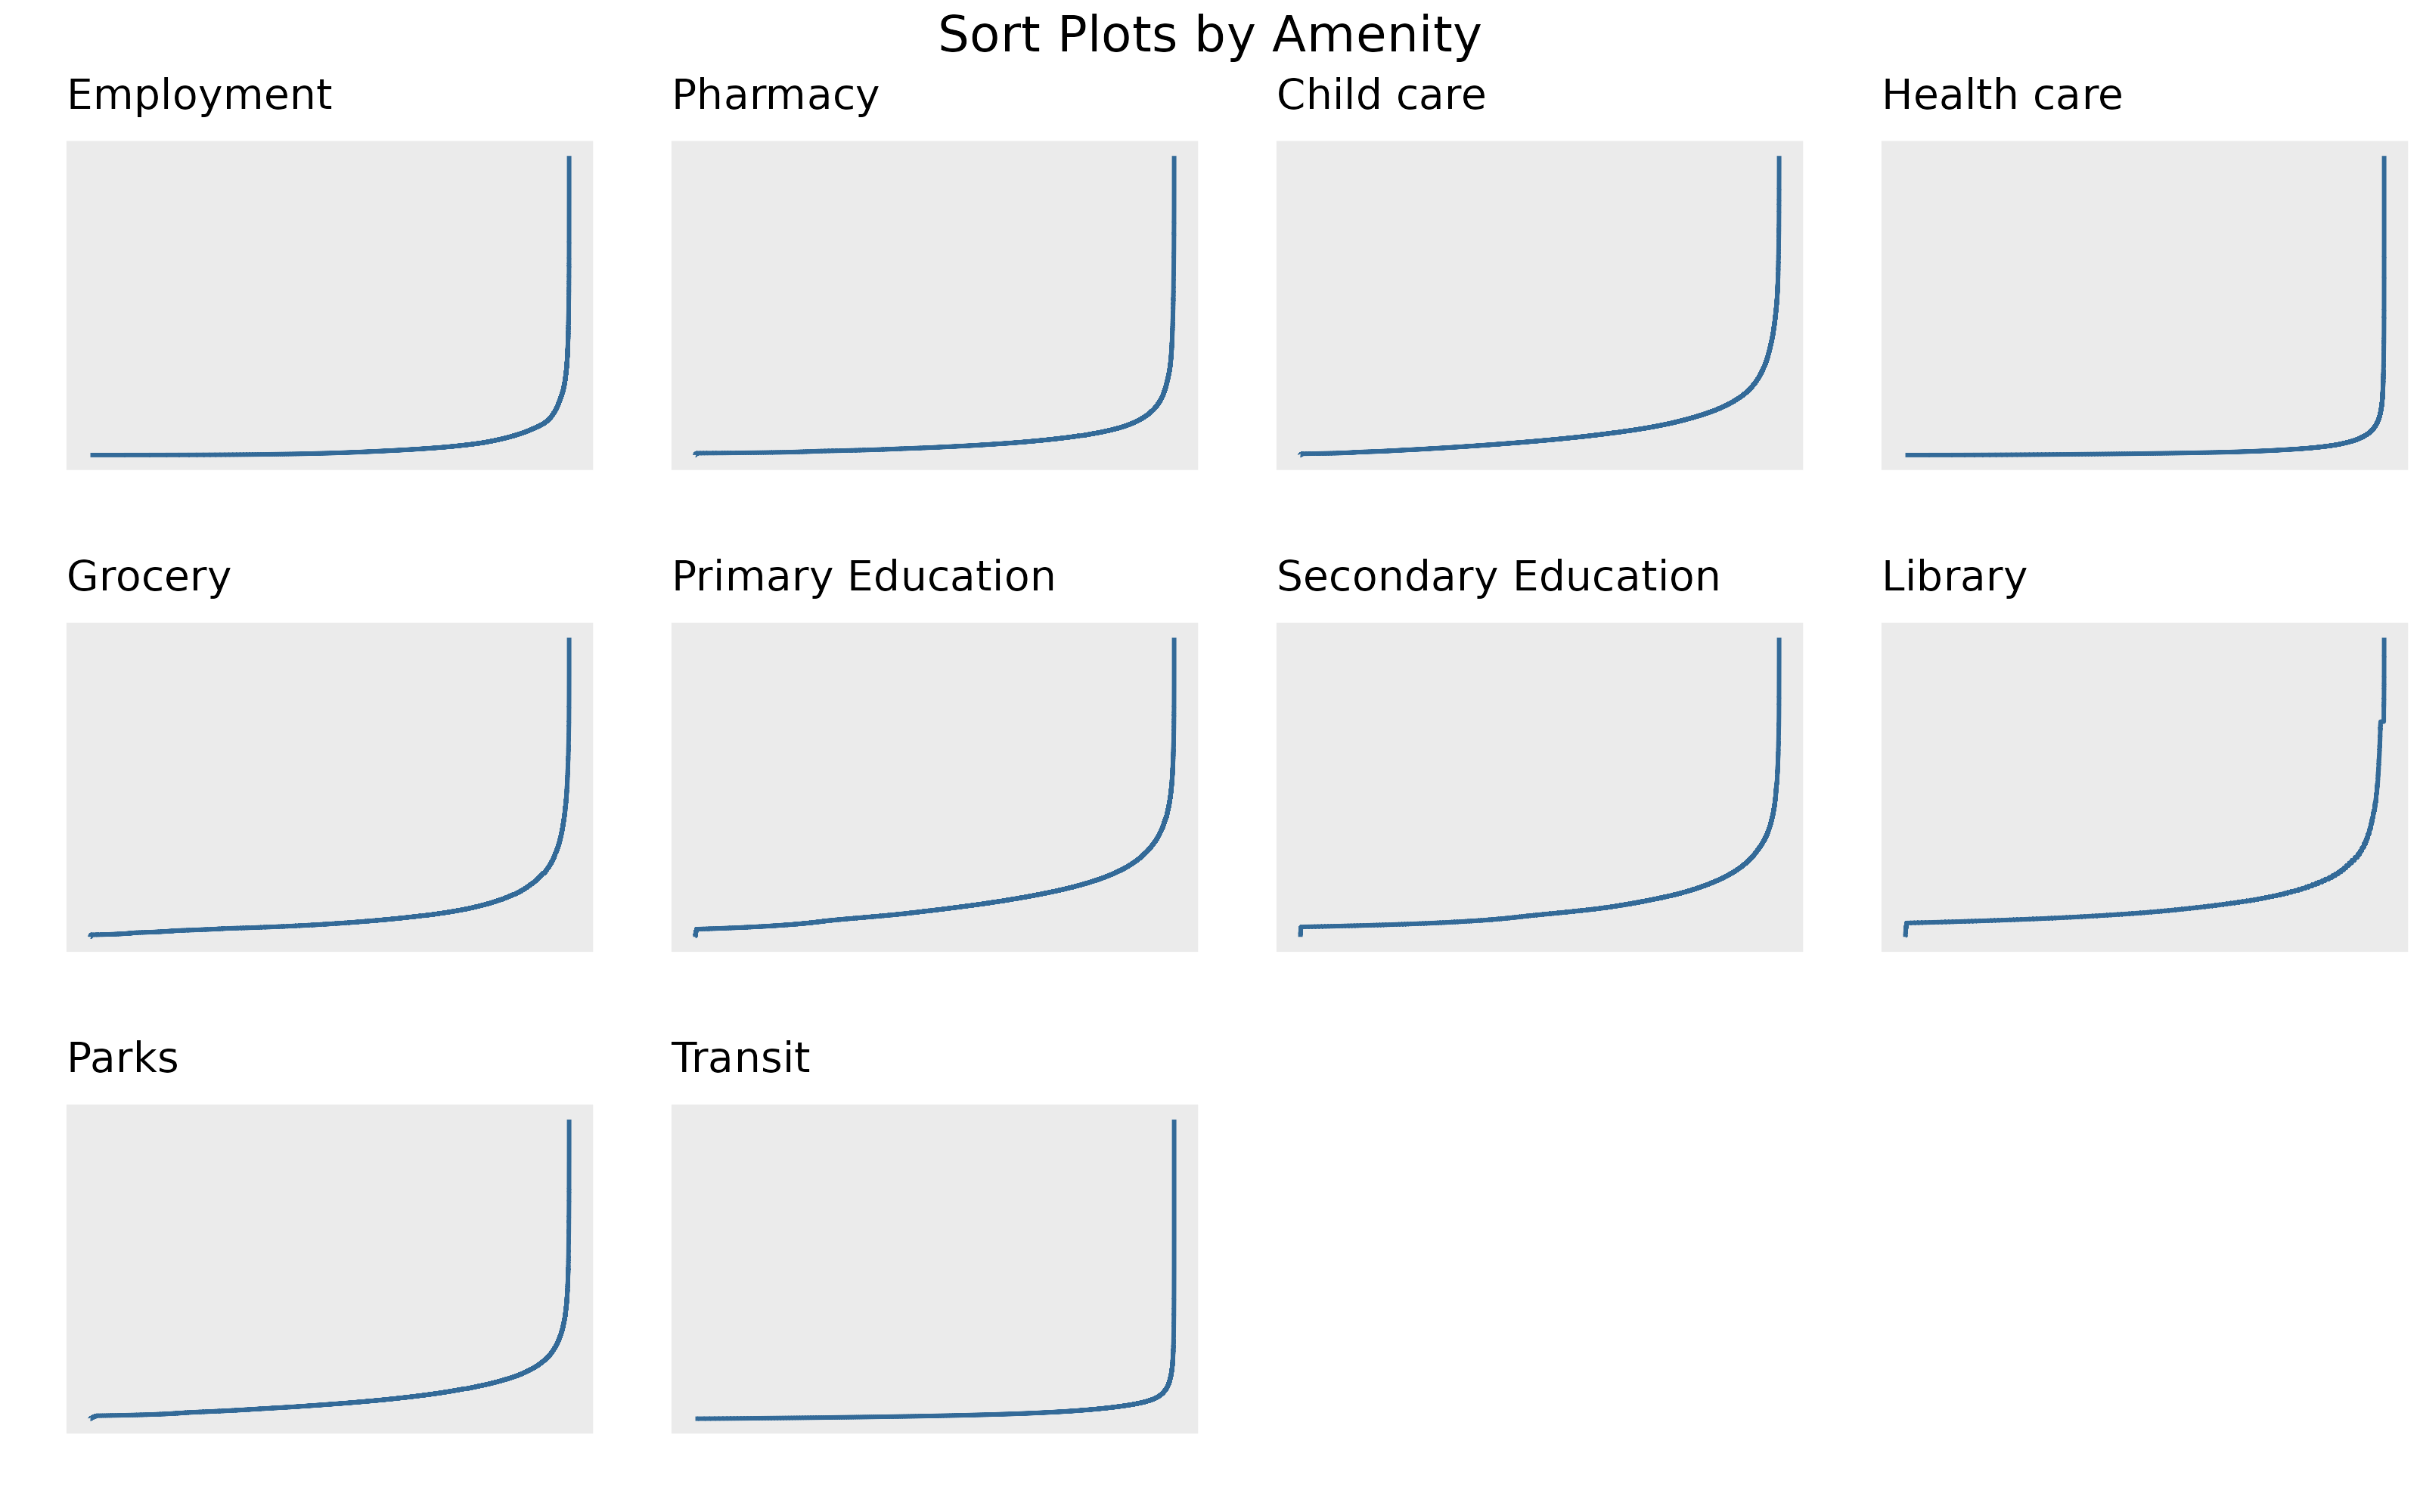
\includegraphics[width=\textwidth]{./sort_plot/sort_plot.png}
\caption[Sort plots]{Sort plots for each amenity in the PMD. }\label{sortplots}
\end{figure}







\begin{figure}[H]
\centering
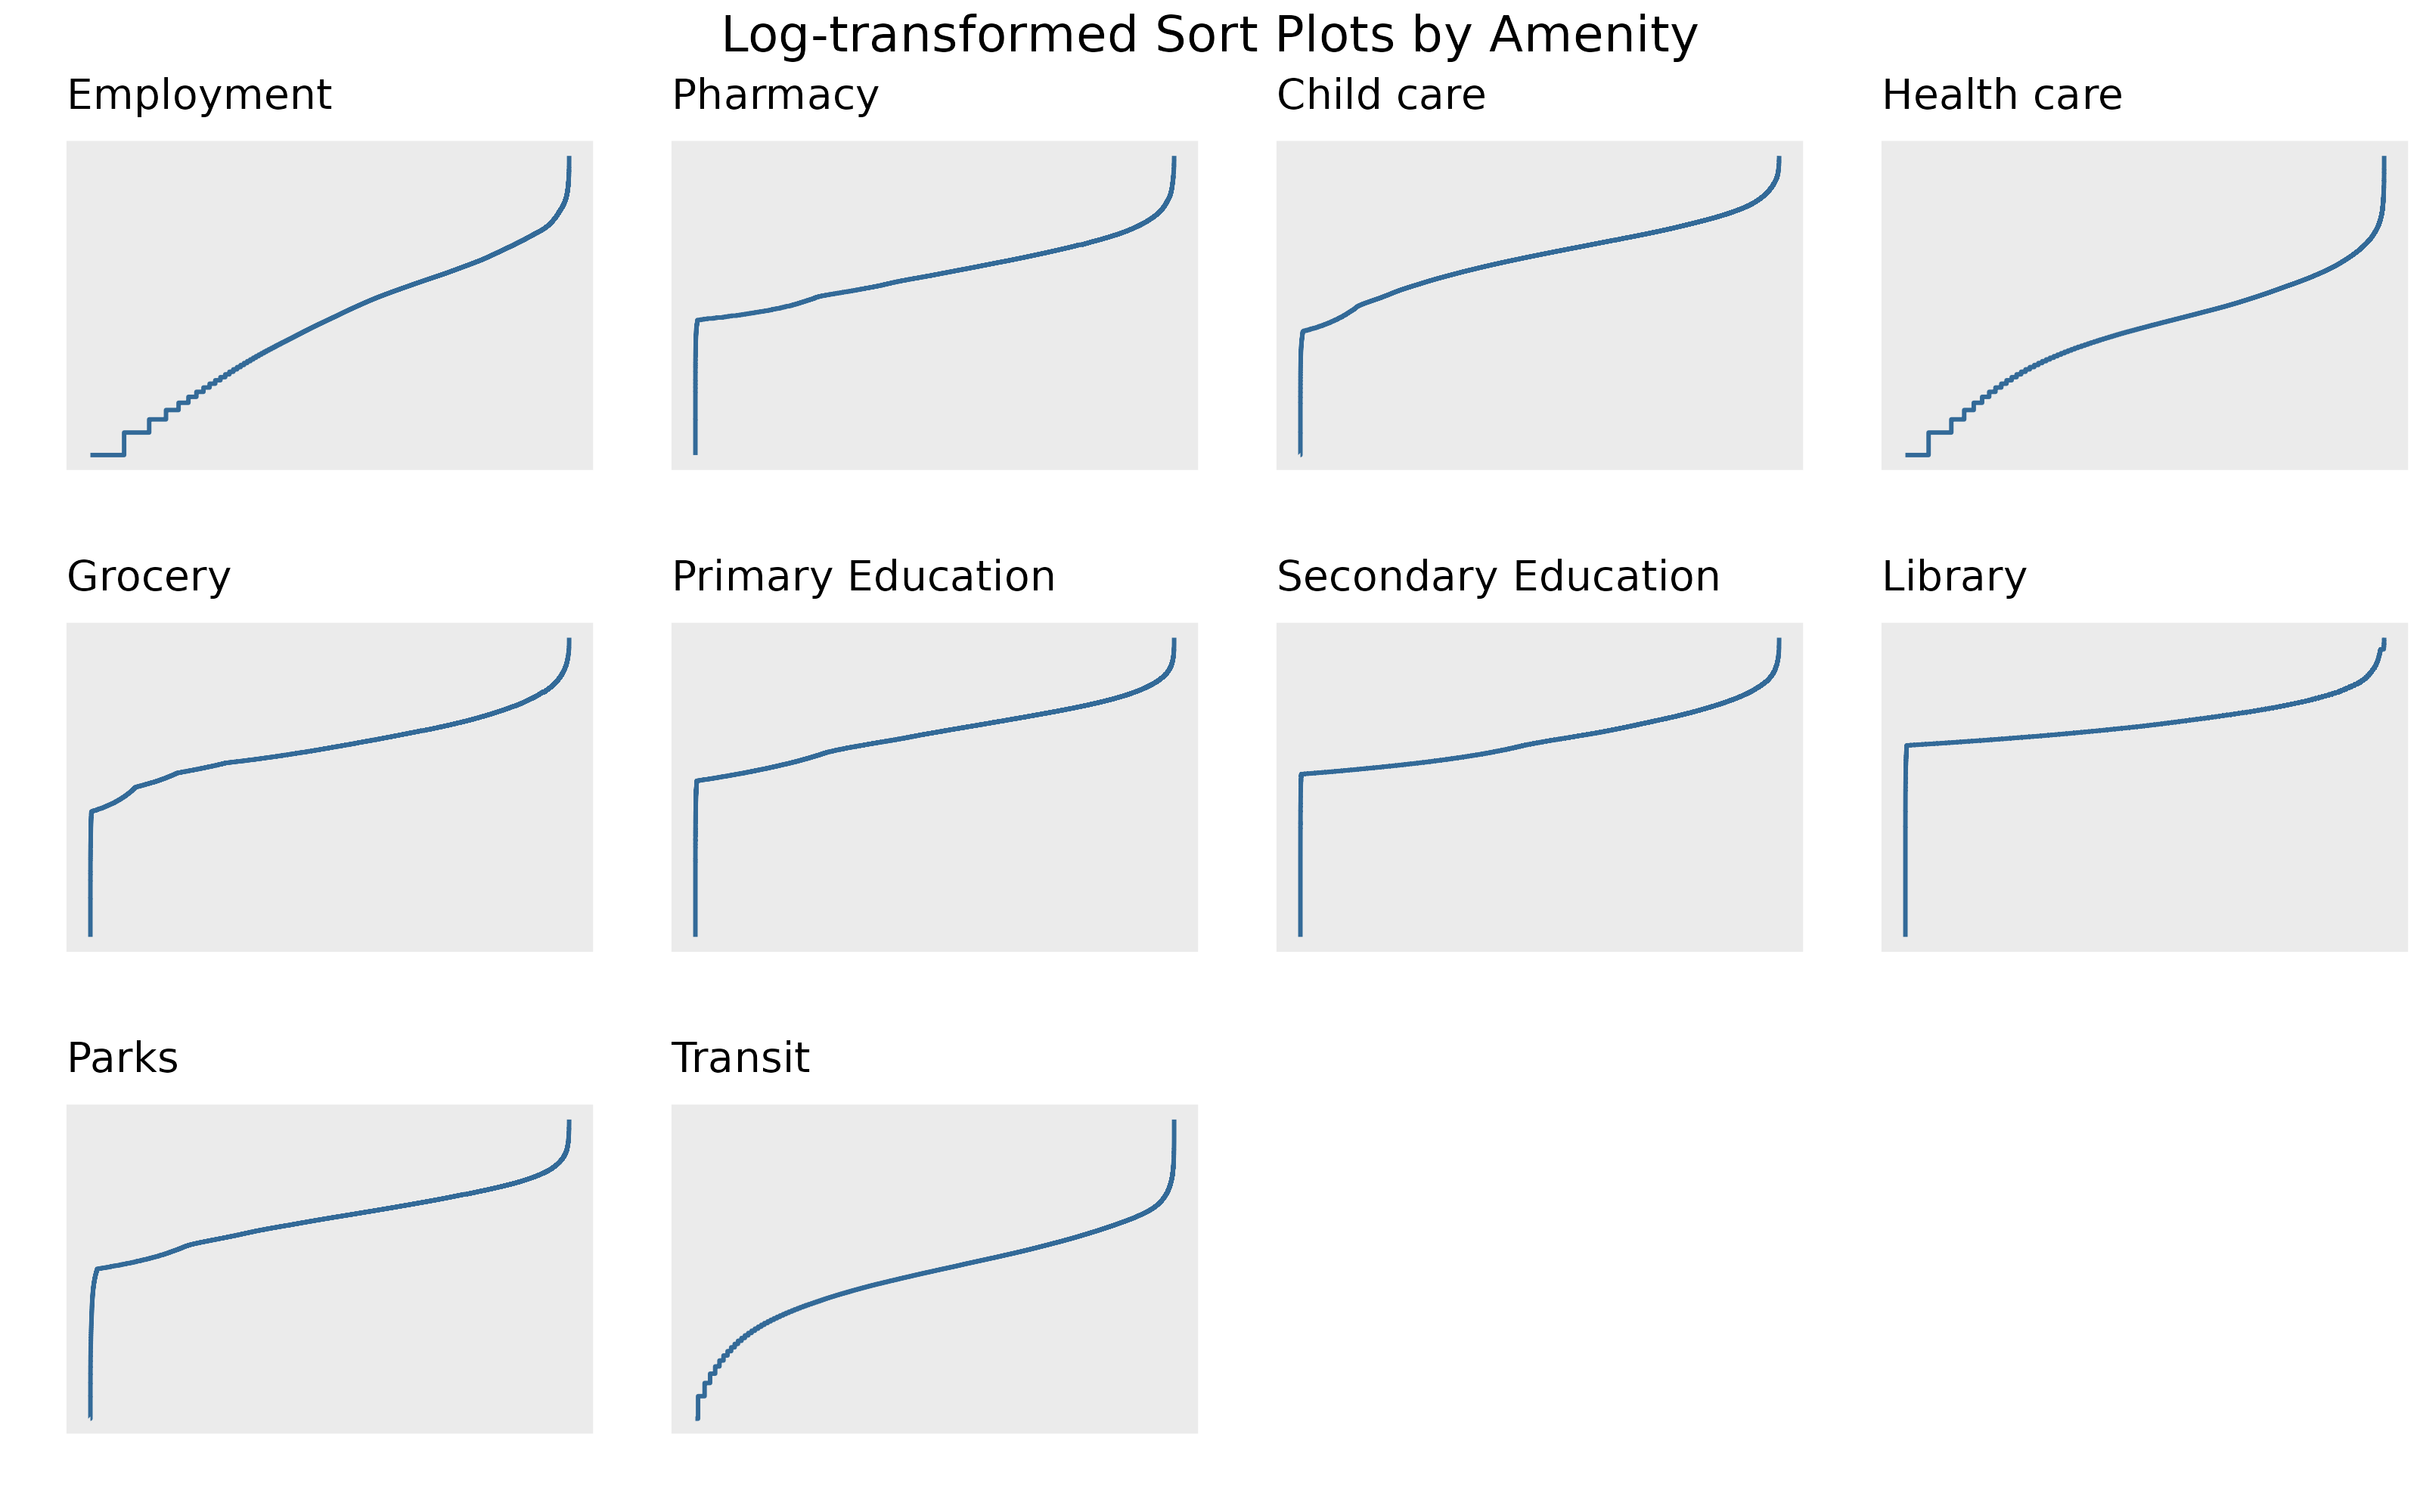
\includegraphics[width=\textwidth]{./sort_plot/log_sort_plot.png}
\caption[Log sort plots]{Log-transformed sort plots for each amenity in the PMD. 
}\label{logsortplots}
\end{figure}







\begin{figure}[H]
\centering
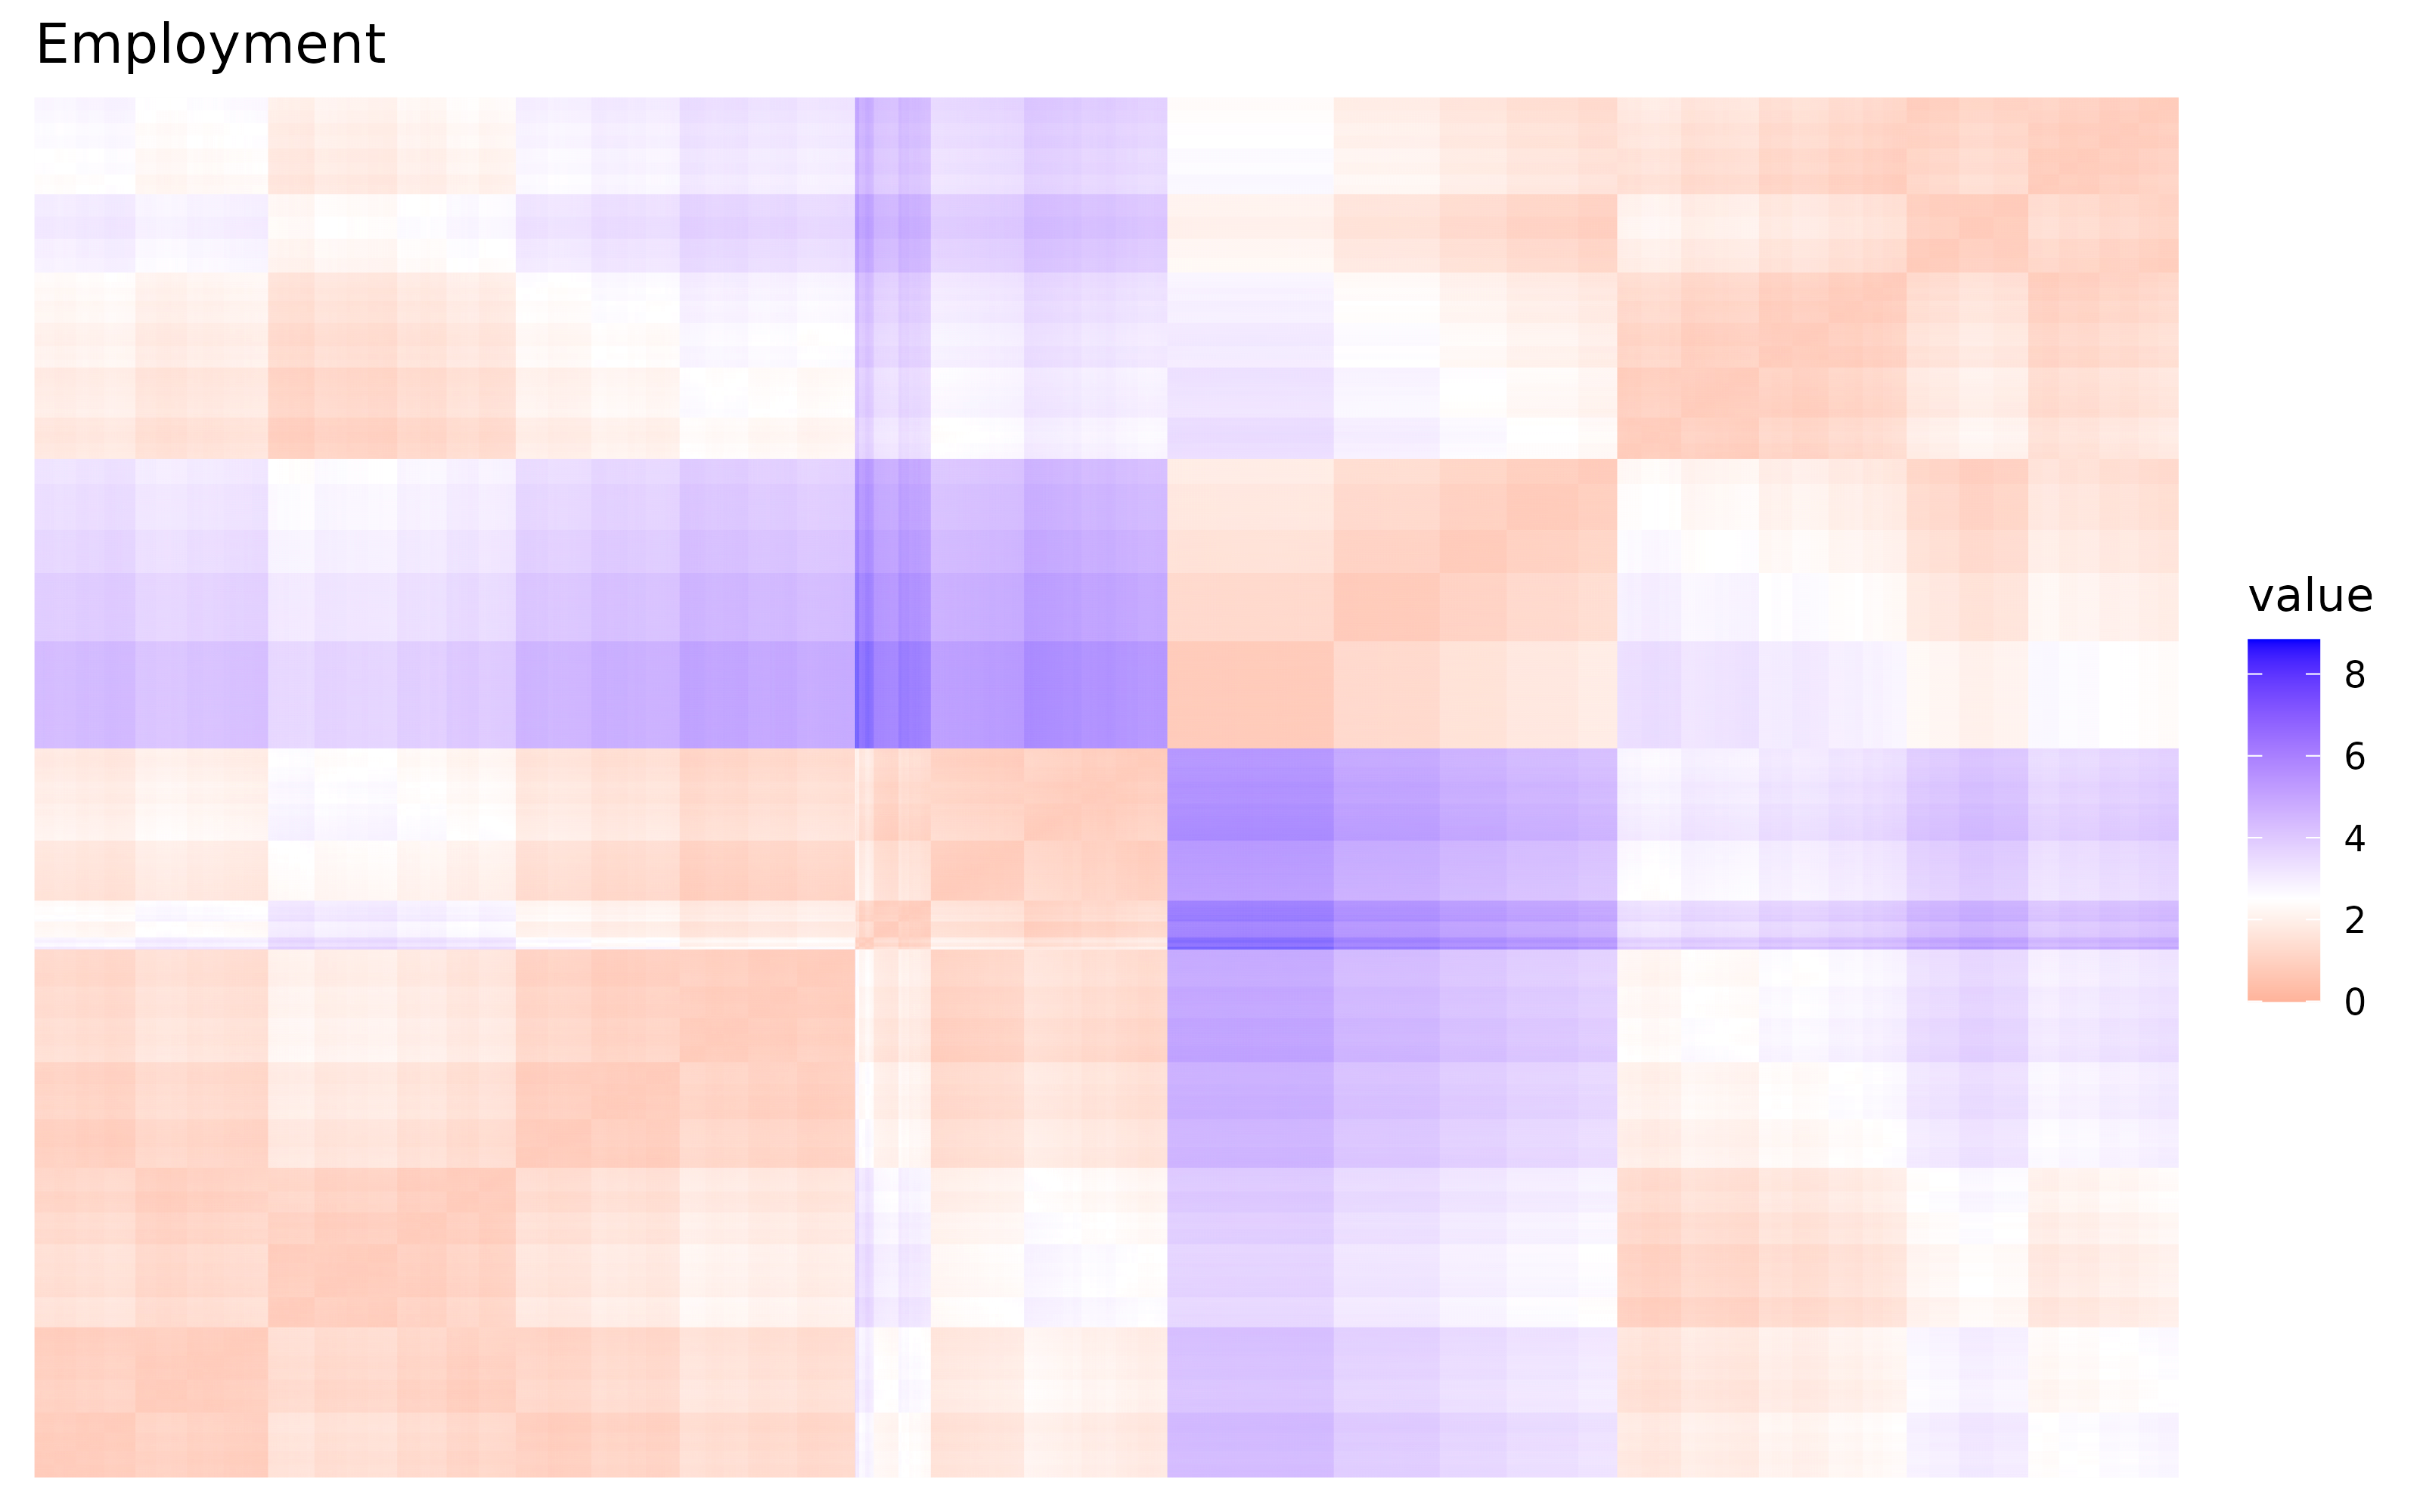
\includegraphics[width=\textwidth]{./vat/emp_vat_log.png}
\caption[Employment VAT plot]{VAT plot for the log-transformed employment amenity.}\label{empvat}
\end{figure}








\begin{figure}[H]
\centering
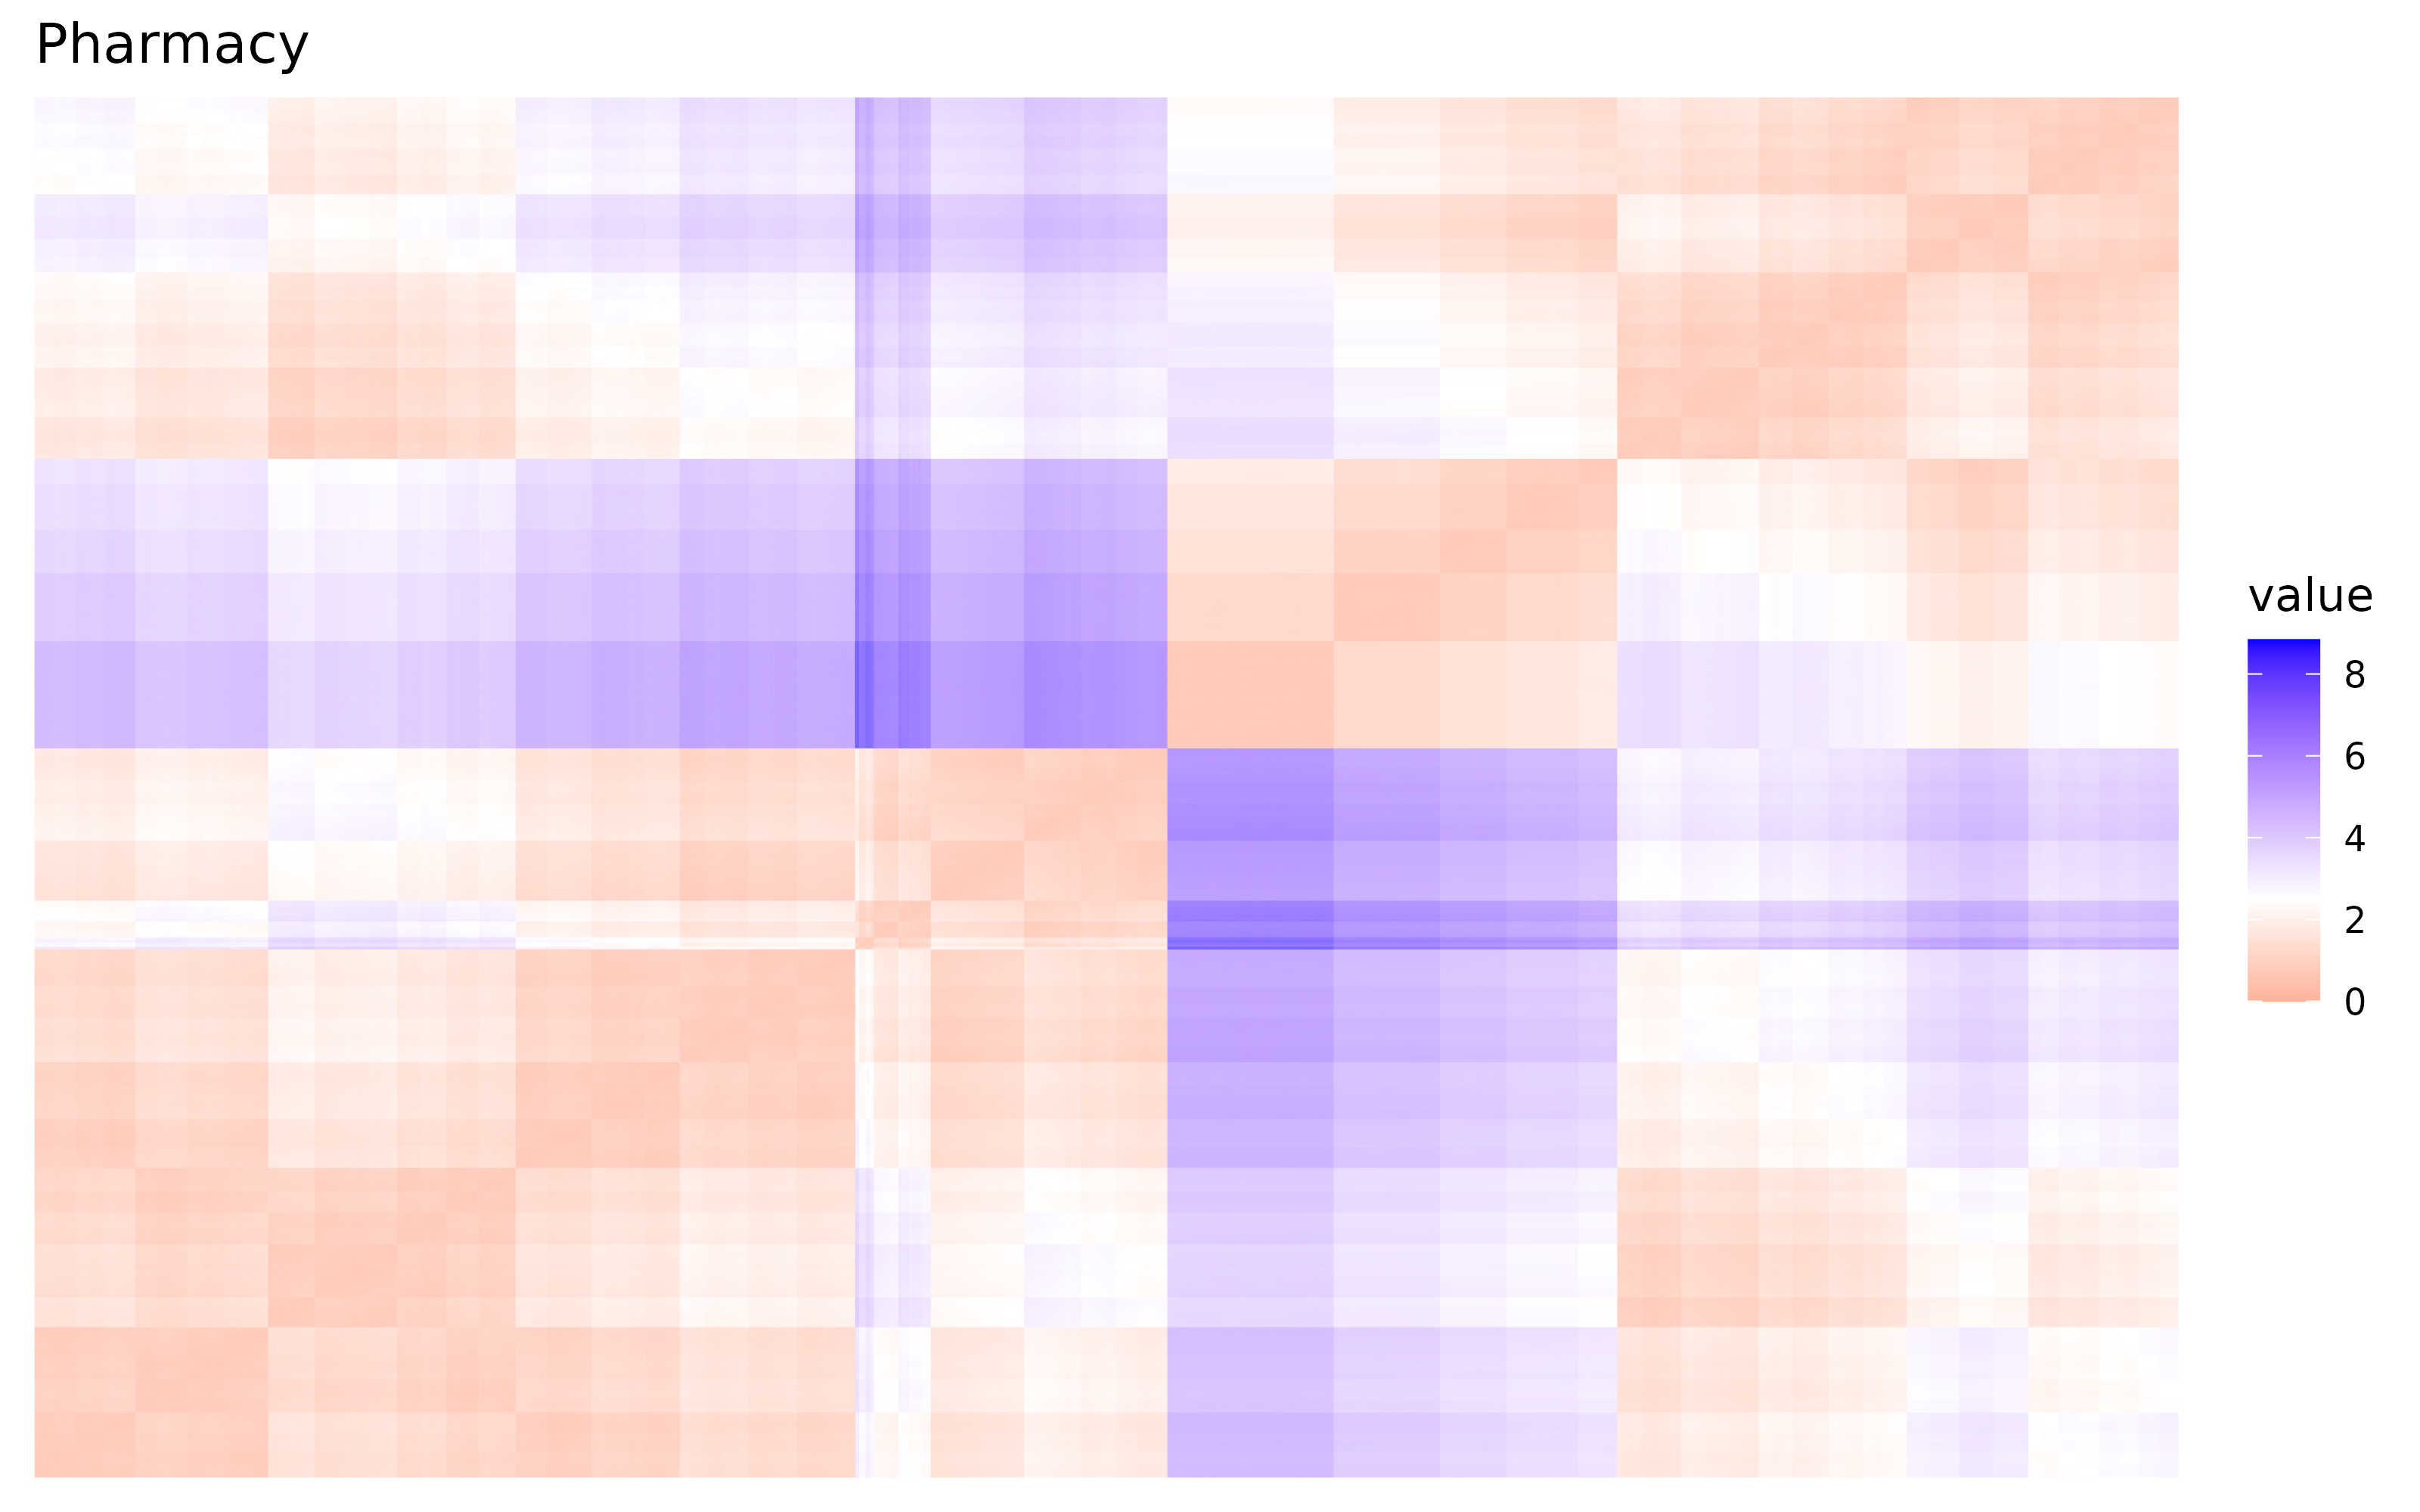
\includegraphics[width=\textwidth]{./vat/pharma_vat_log.png}
\caption[Pharmacy VAT plot]{VAT plot for the log-transformed pharmacy amenity.}\label{pharmavat}
\end{figure}






\begin{figure}[H]
\centering
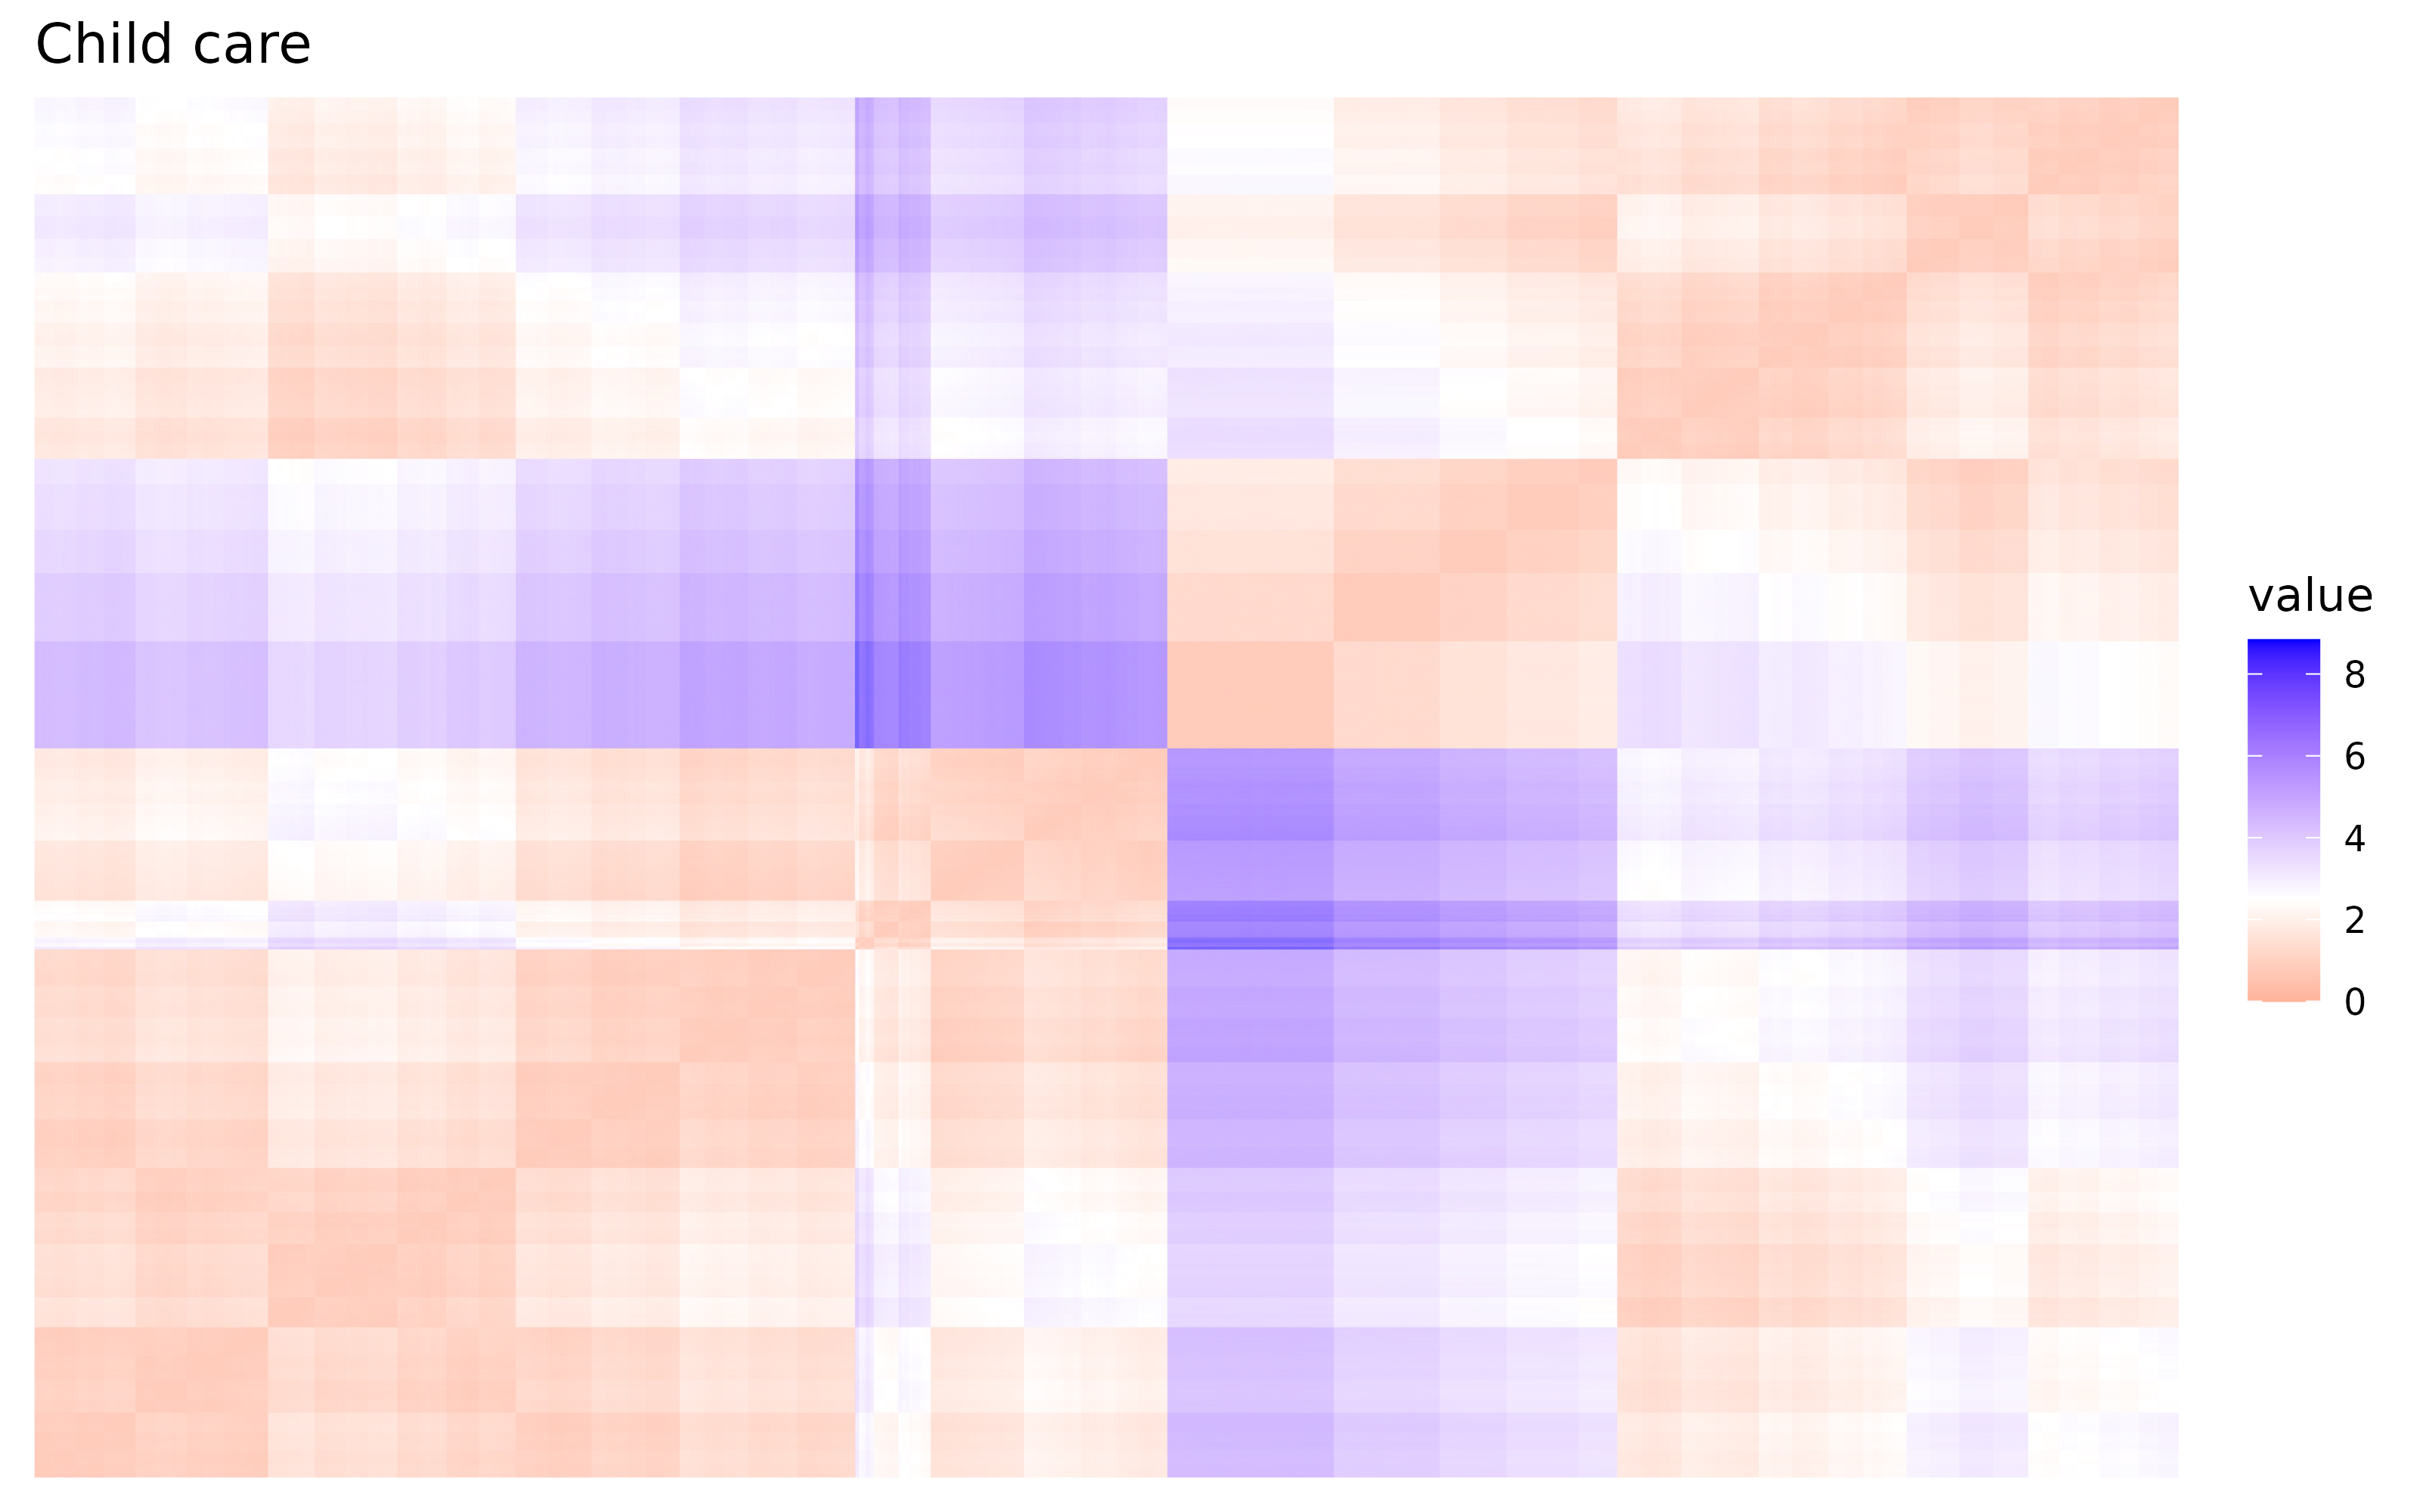
\includegraphics[width=\textwidth]{./vat/childcare_vat_log.png}
\caption[Child care VAT plot]{VAT plot for the log-transformed child care amenity.}\label{childcarevat}
\end{figure}








\begin{figure}[H]
\centering
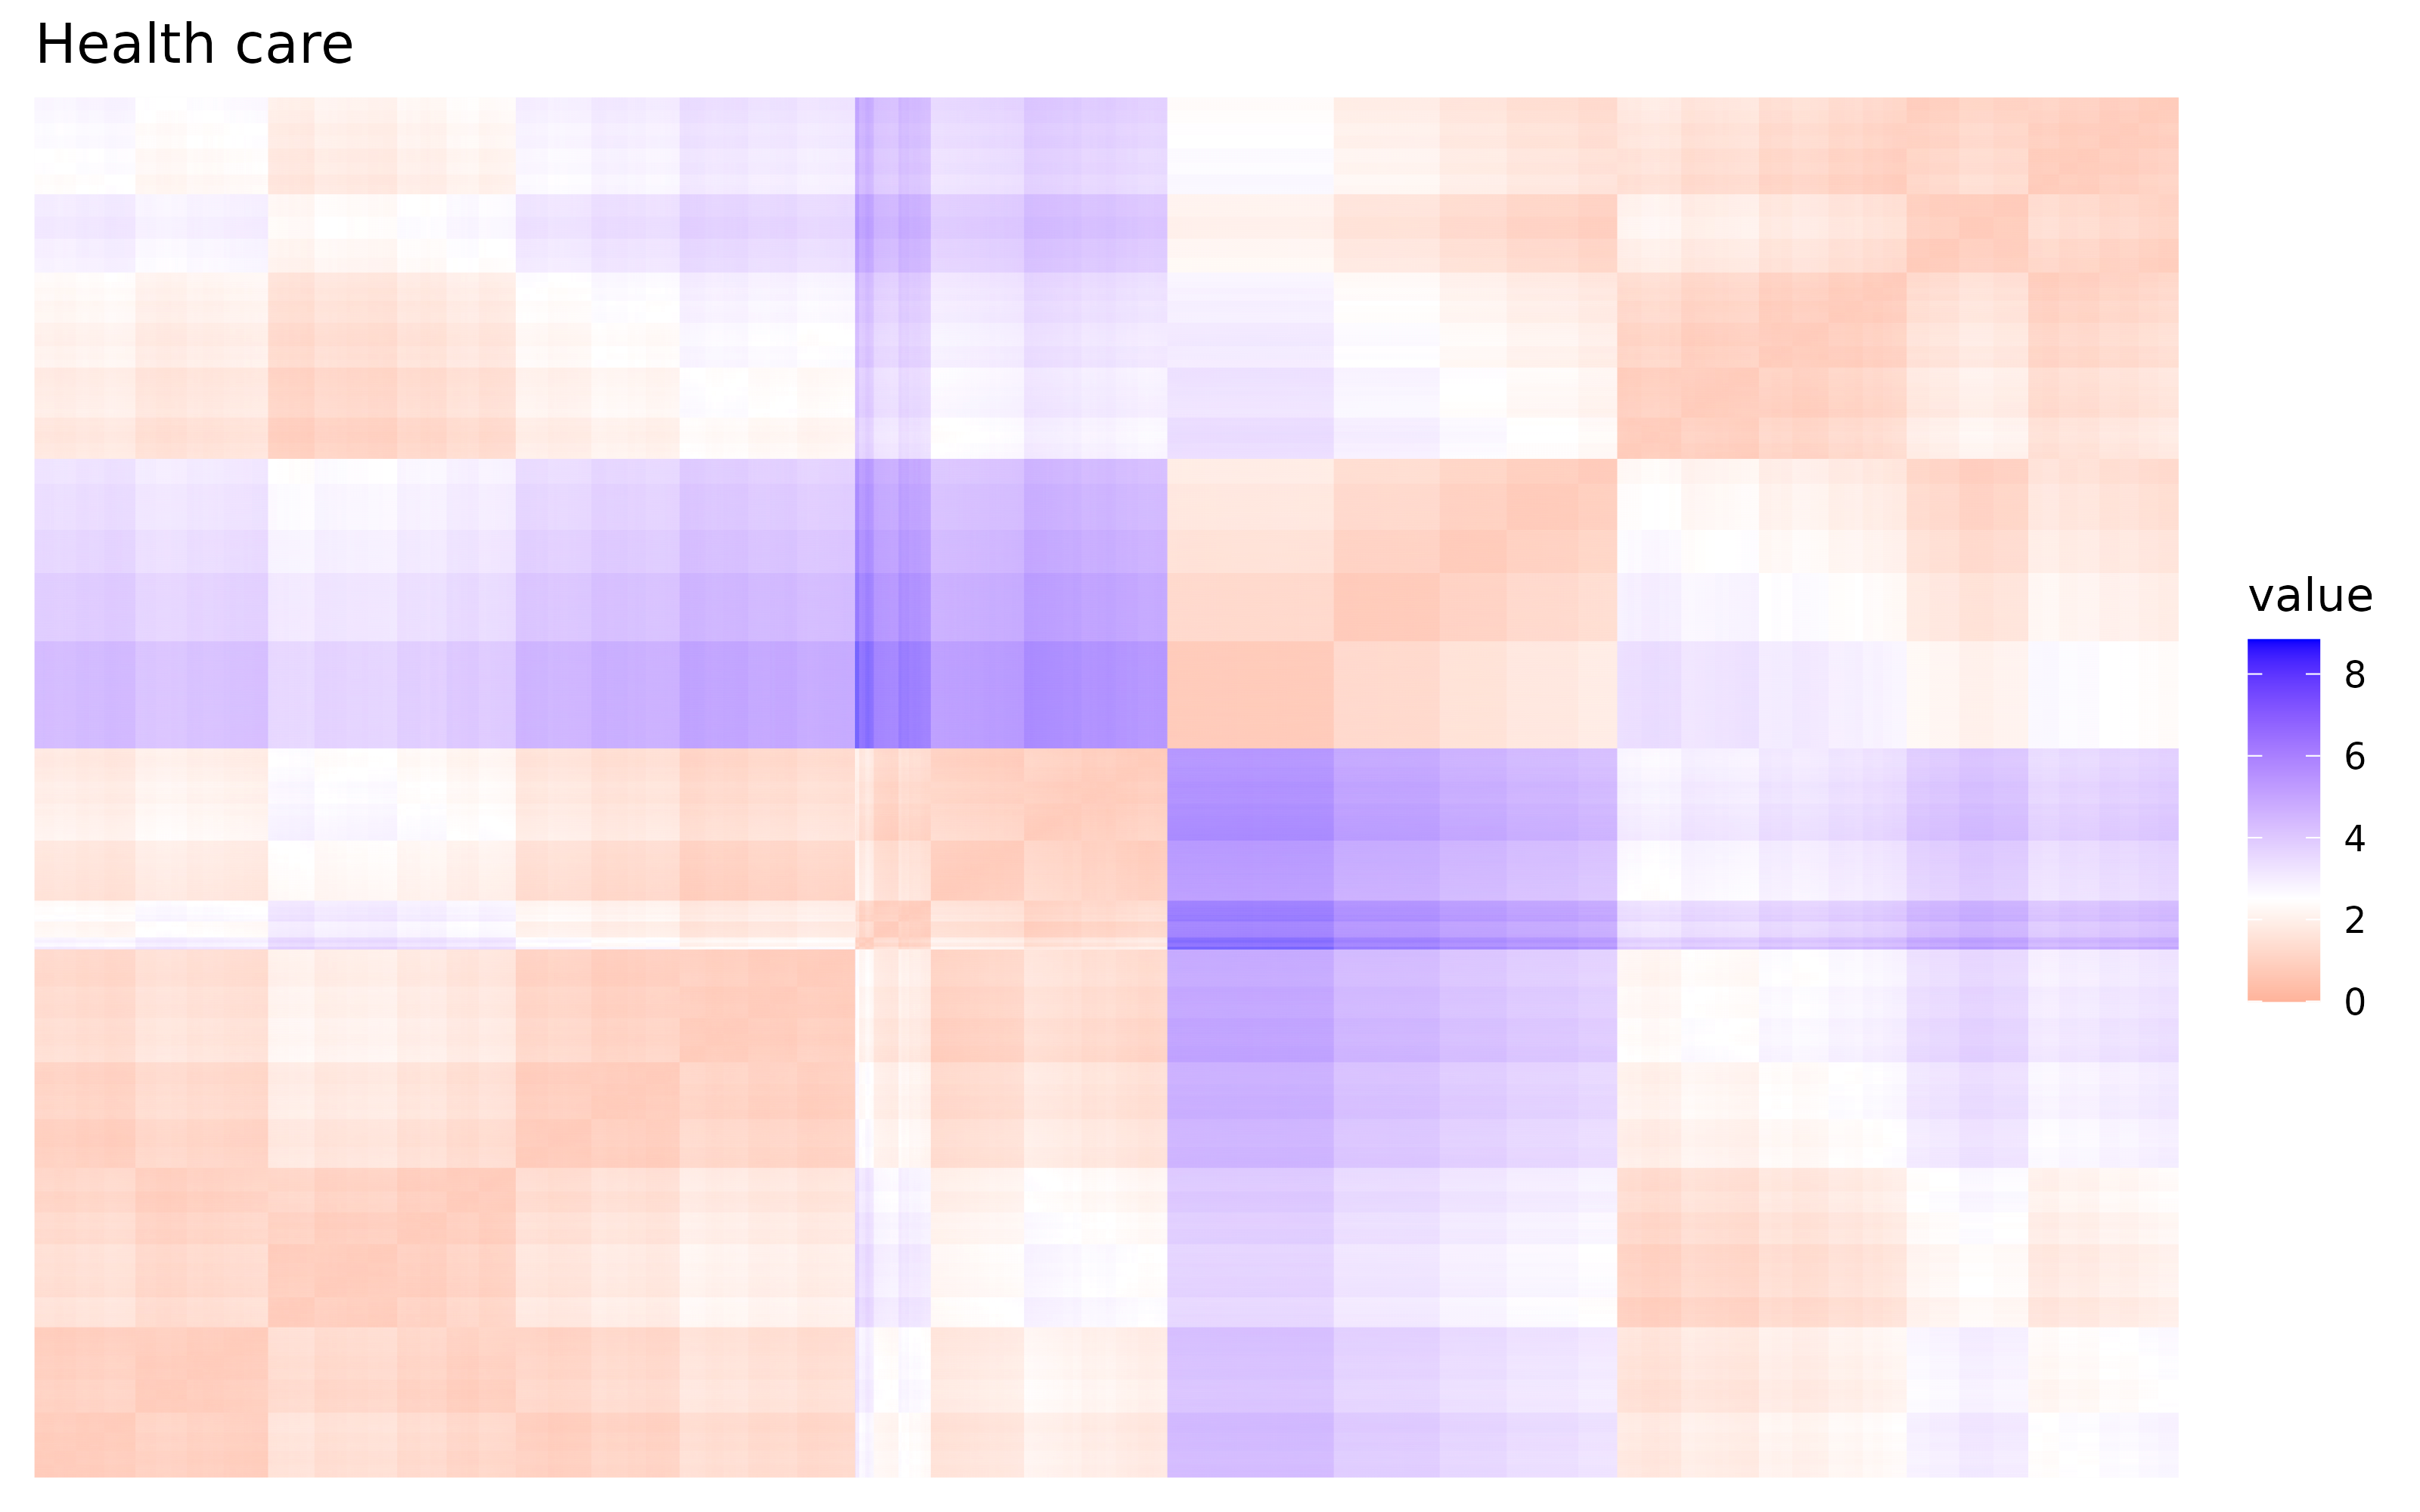
\includegraphics[width=\textwidth]{./vat/healthcare_vat_log.png}
\caption[Health care VAT plot]{VAT plot for the log-transformed health care amenity.}\label{healthcarevat}
\end{figure}







\begin{figure}[H]
\centering
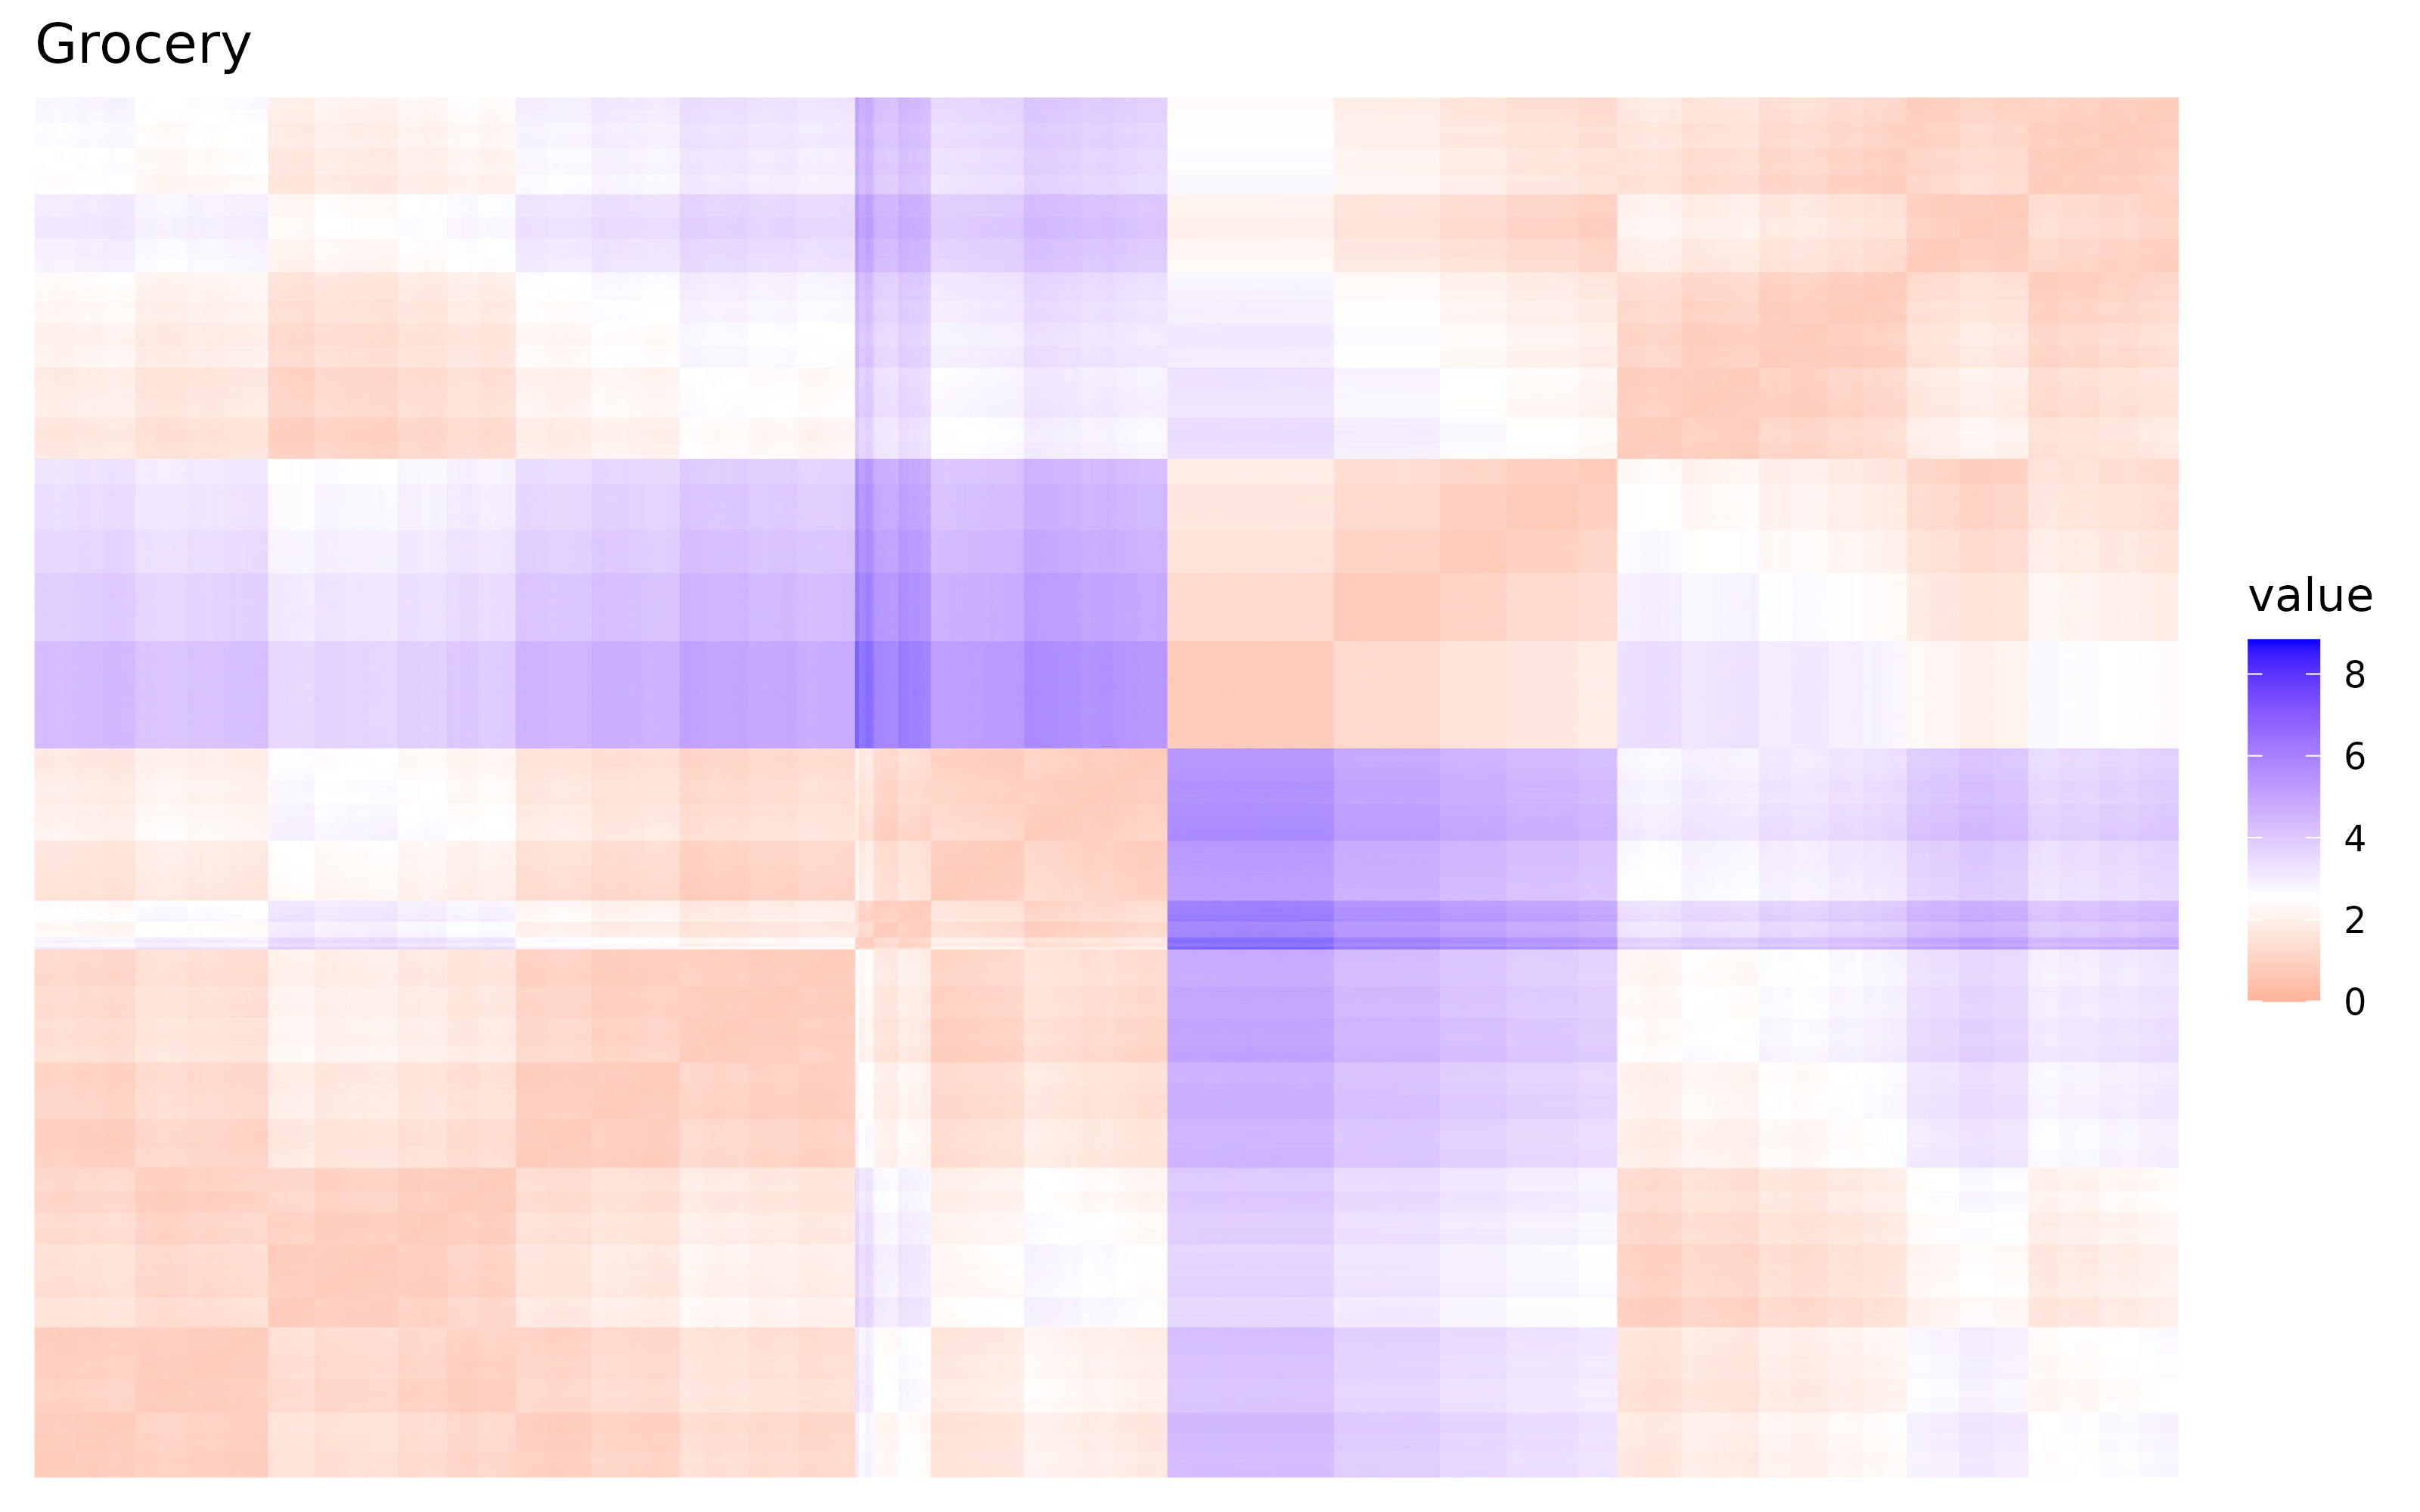
\includegraphics[width=\textwidth]{./vat/grocery_vat_log.png}
\caption[Grocery VAT plot]{VAT plot for the log-transformed grocery amenity.}\label{groceryvat}
\end{figure}








\begin{figure}[H]
\centering
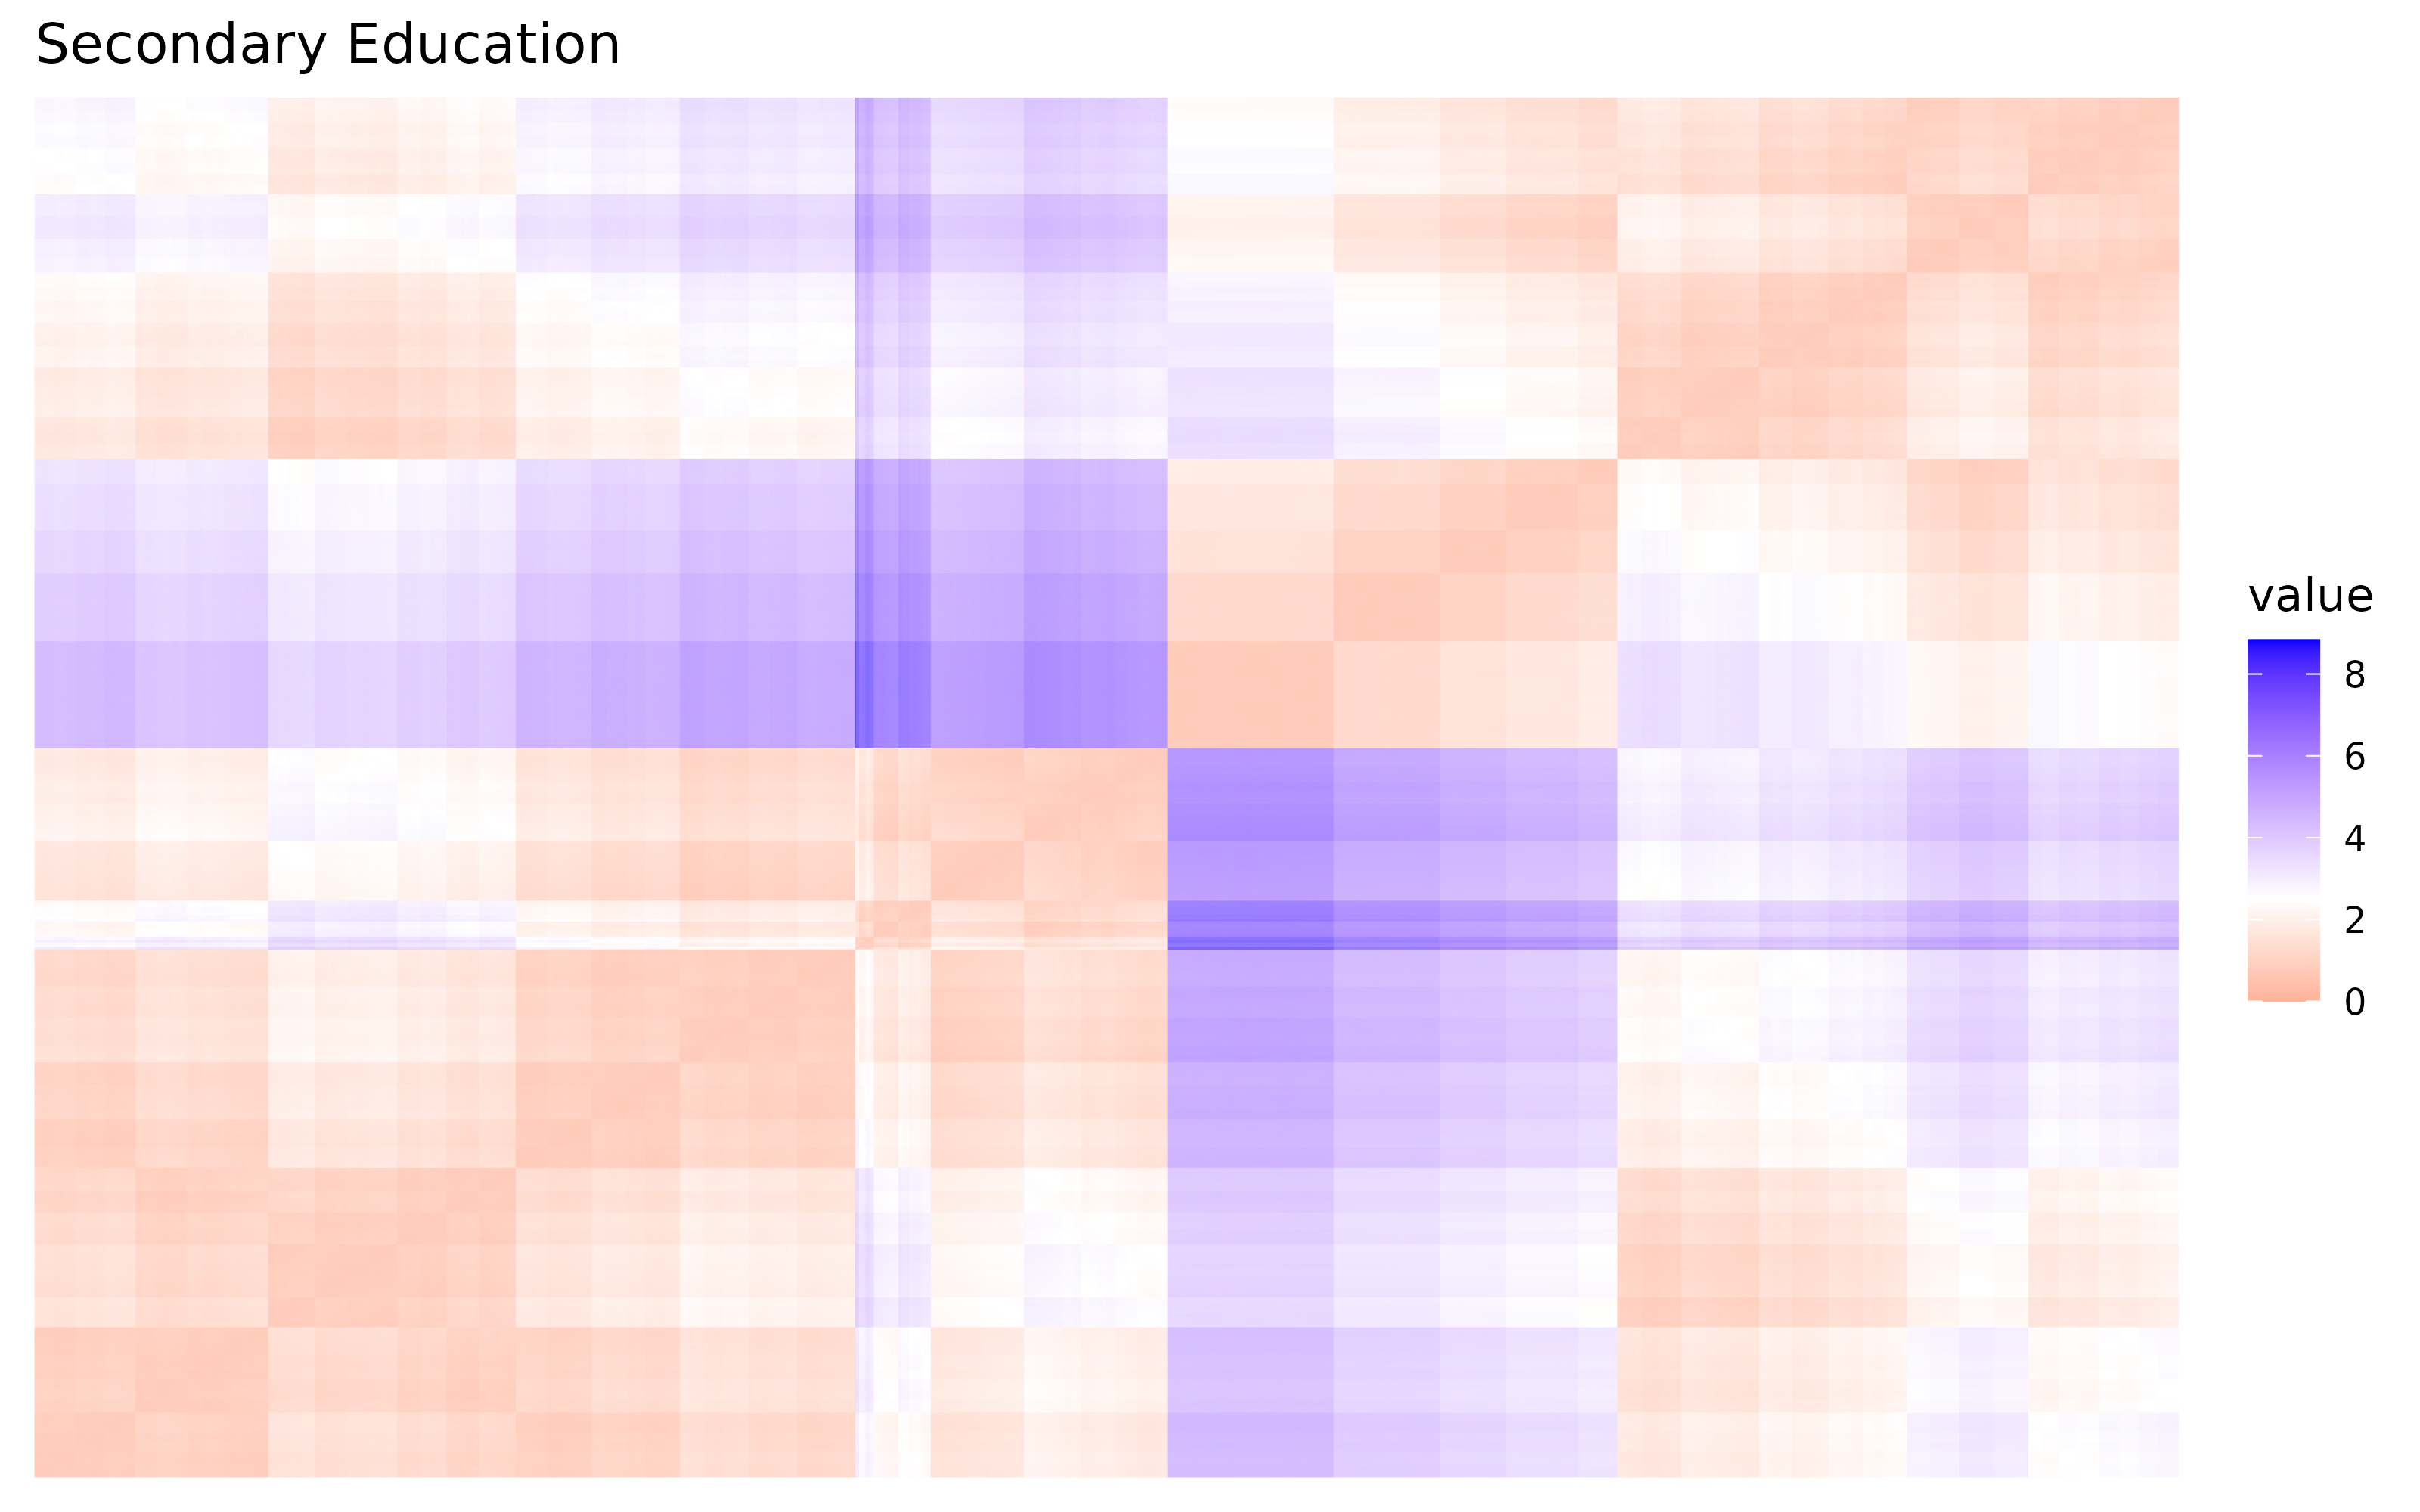
\includegraphics[width=\textwidth]{./vat/secondaryeducation_vat_log.png}
\caption[Secondary education VAT plot]{VAT plot for the log-transformed secondary education amenity.}\label{seceducvat}
\end{figure}








\begin{figure}[H]
\centering
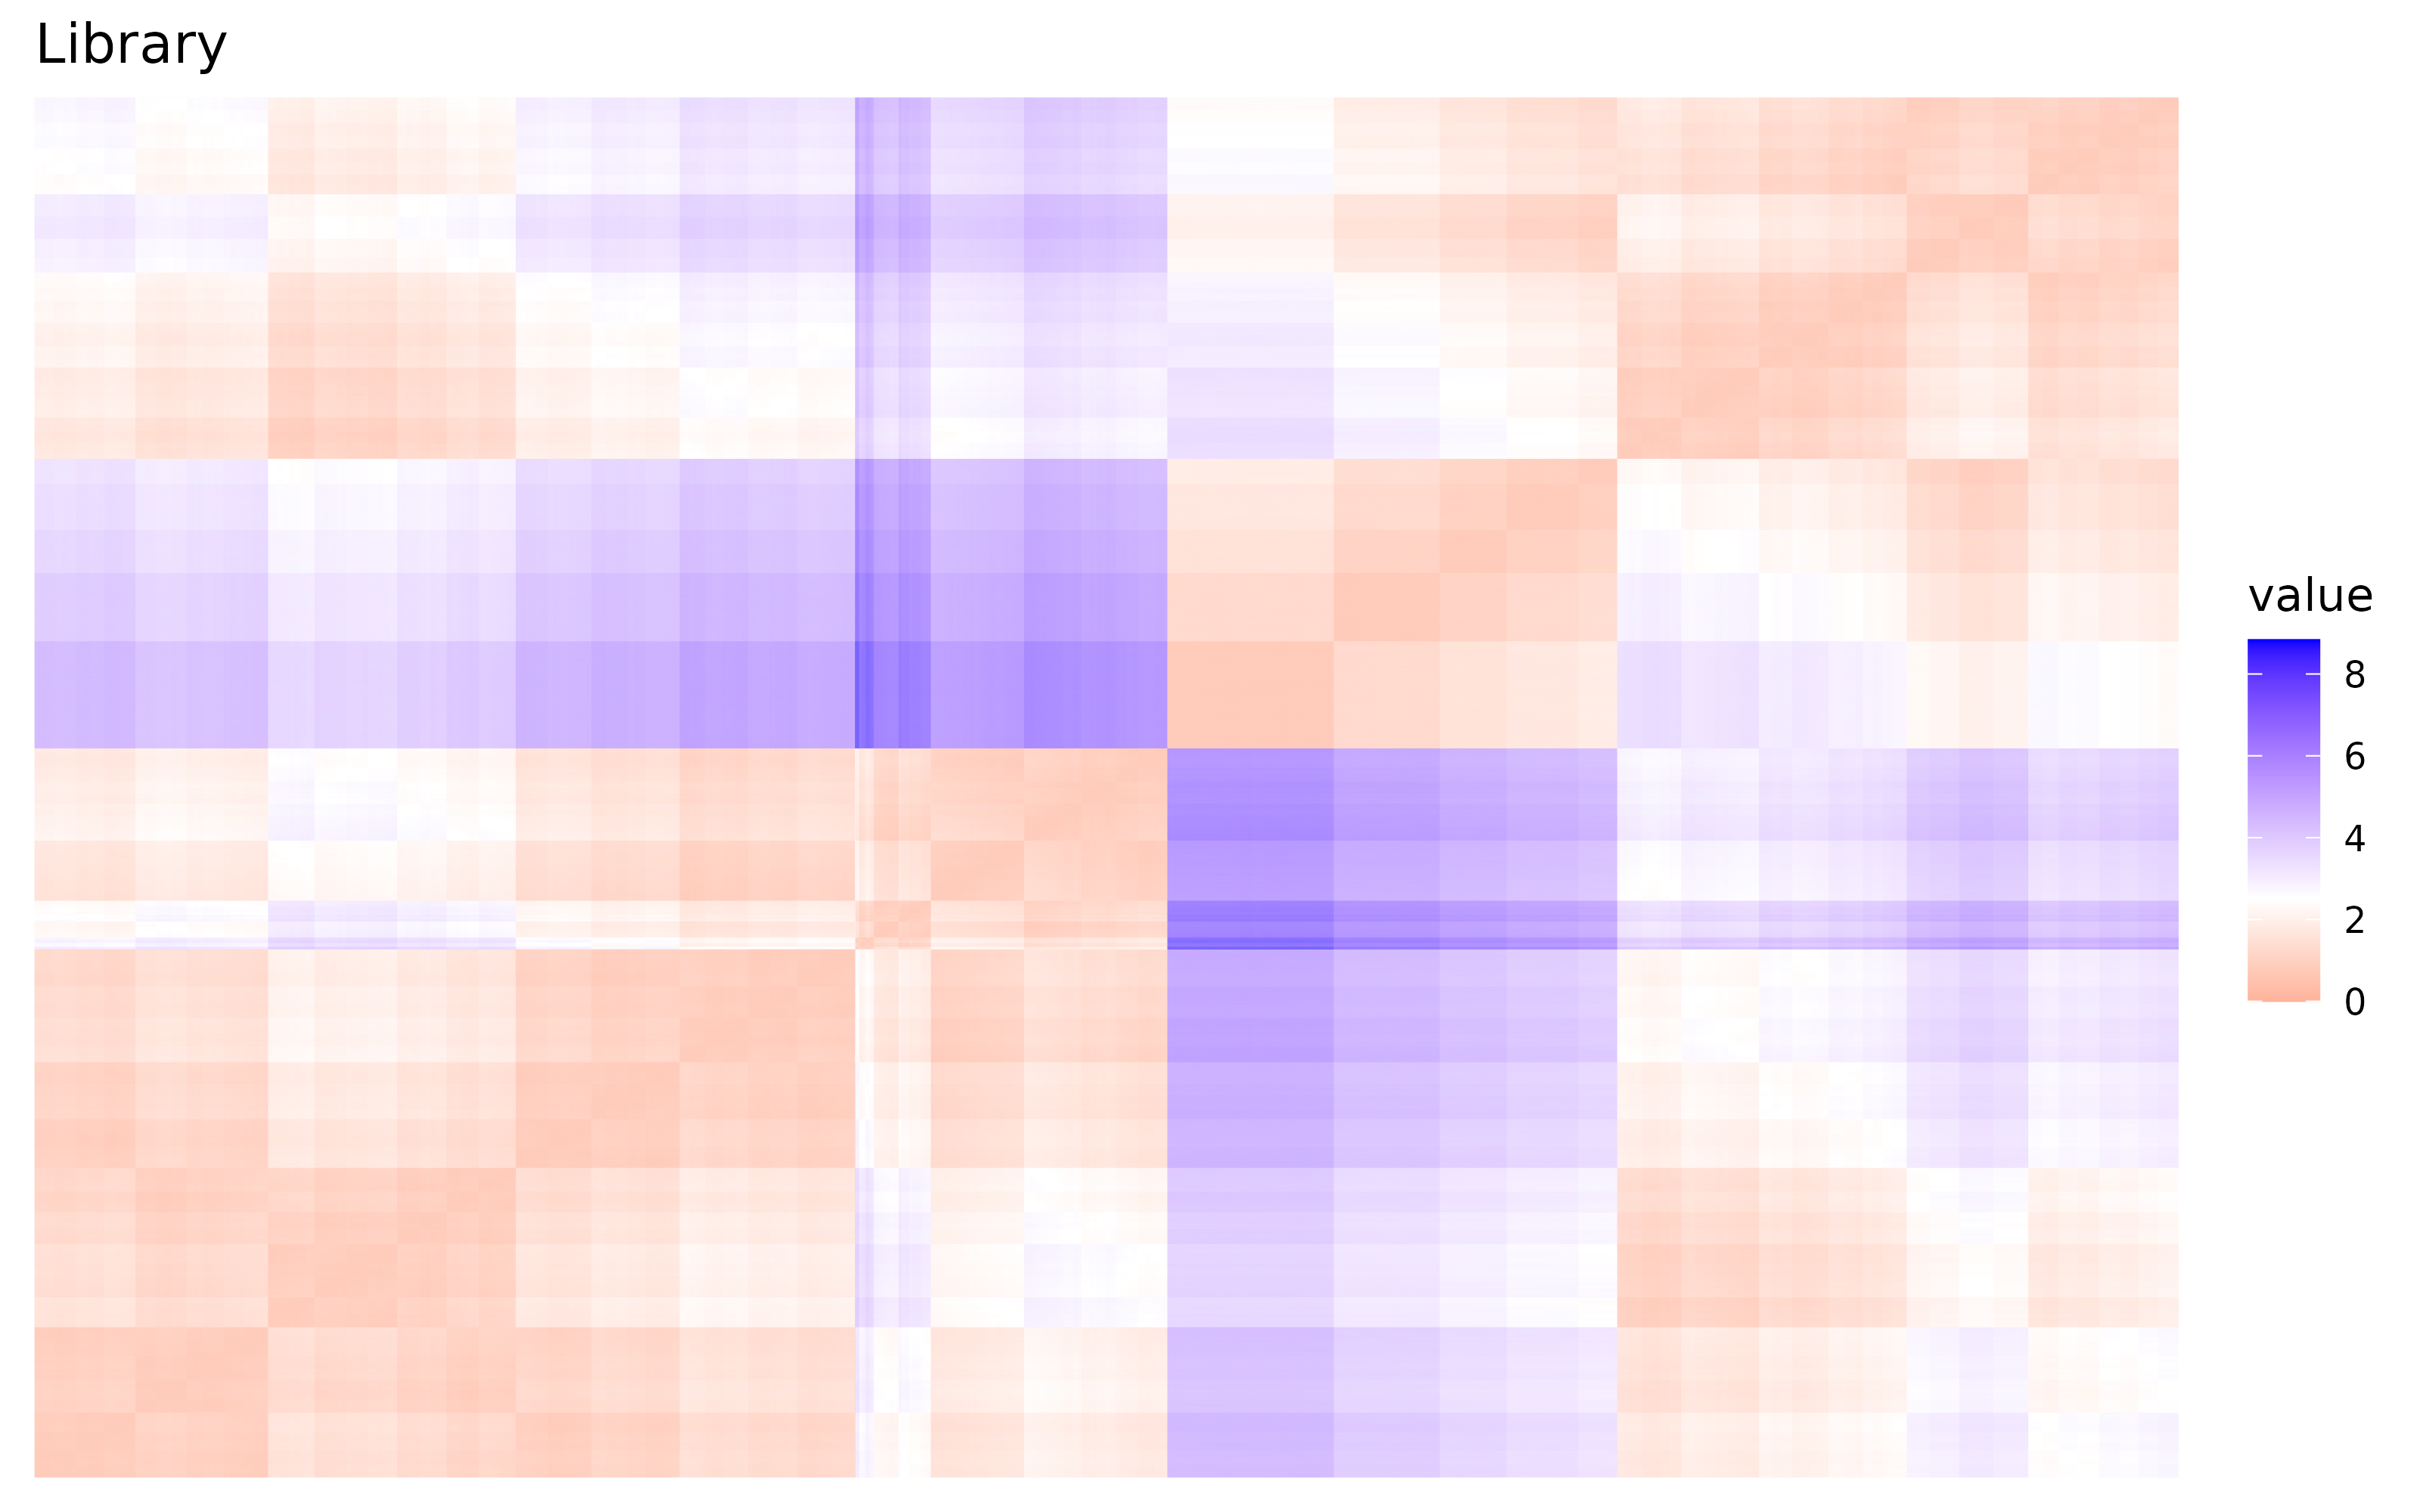
\includegraphics[width=\textwidth]{./vat/library_vat_log.png}
\caption[Library VAT plot]{VAT plot for the log-transformed library amenity.}\label{libraryvat}
\end{figure}








\begin{figure}[H]
\centering
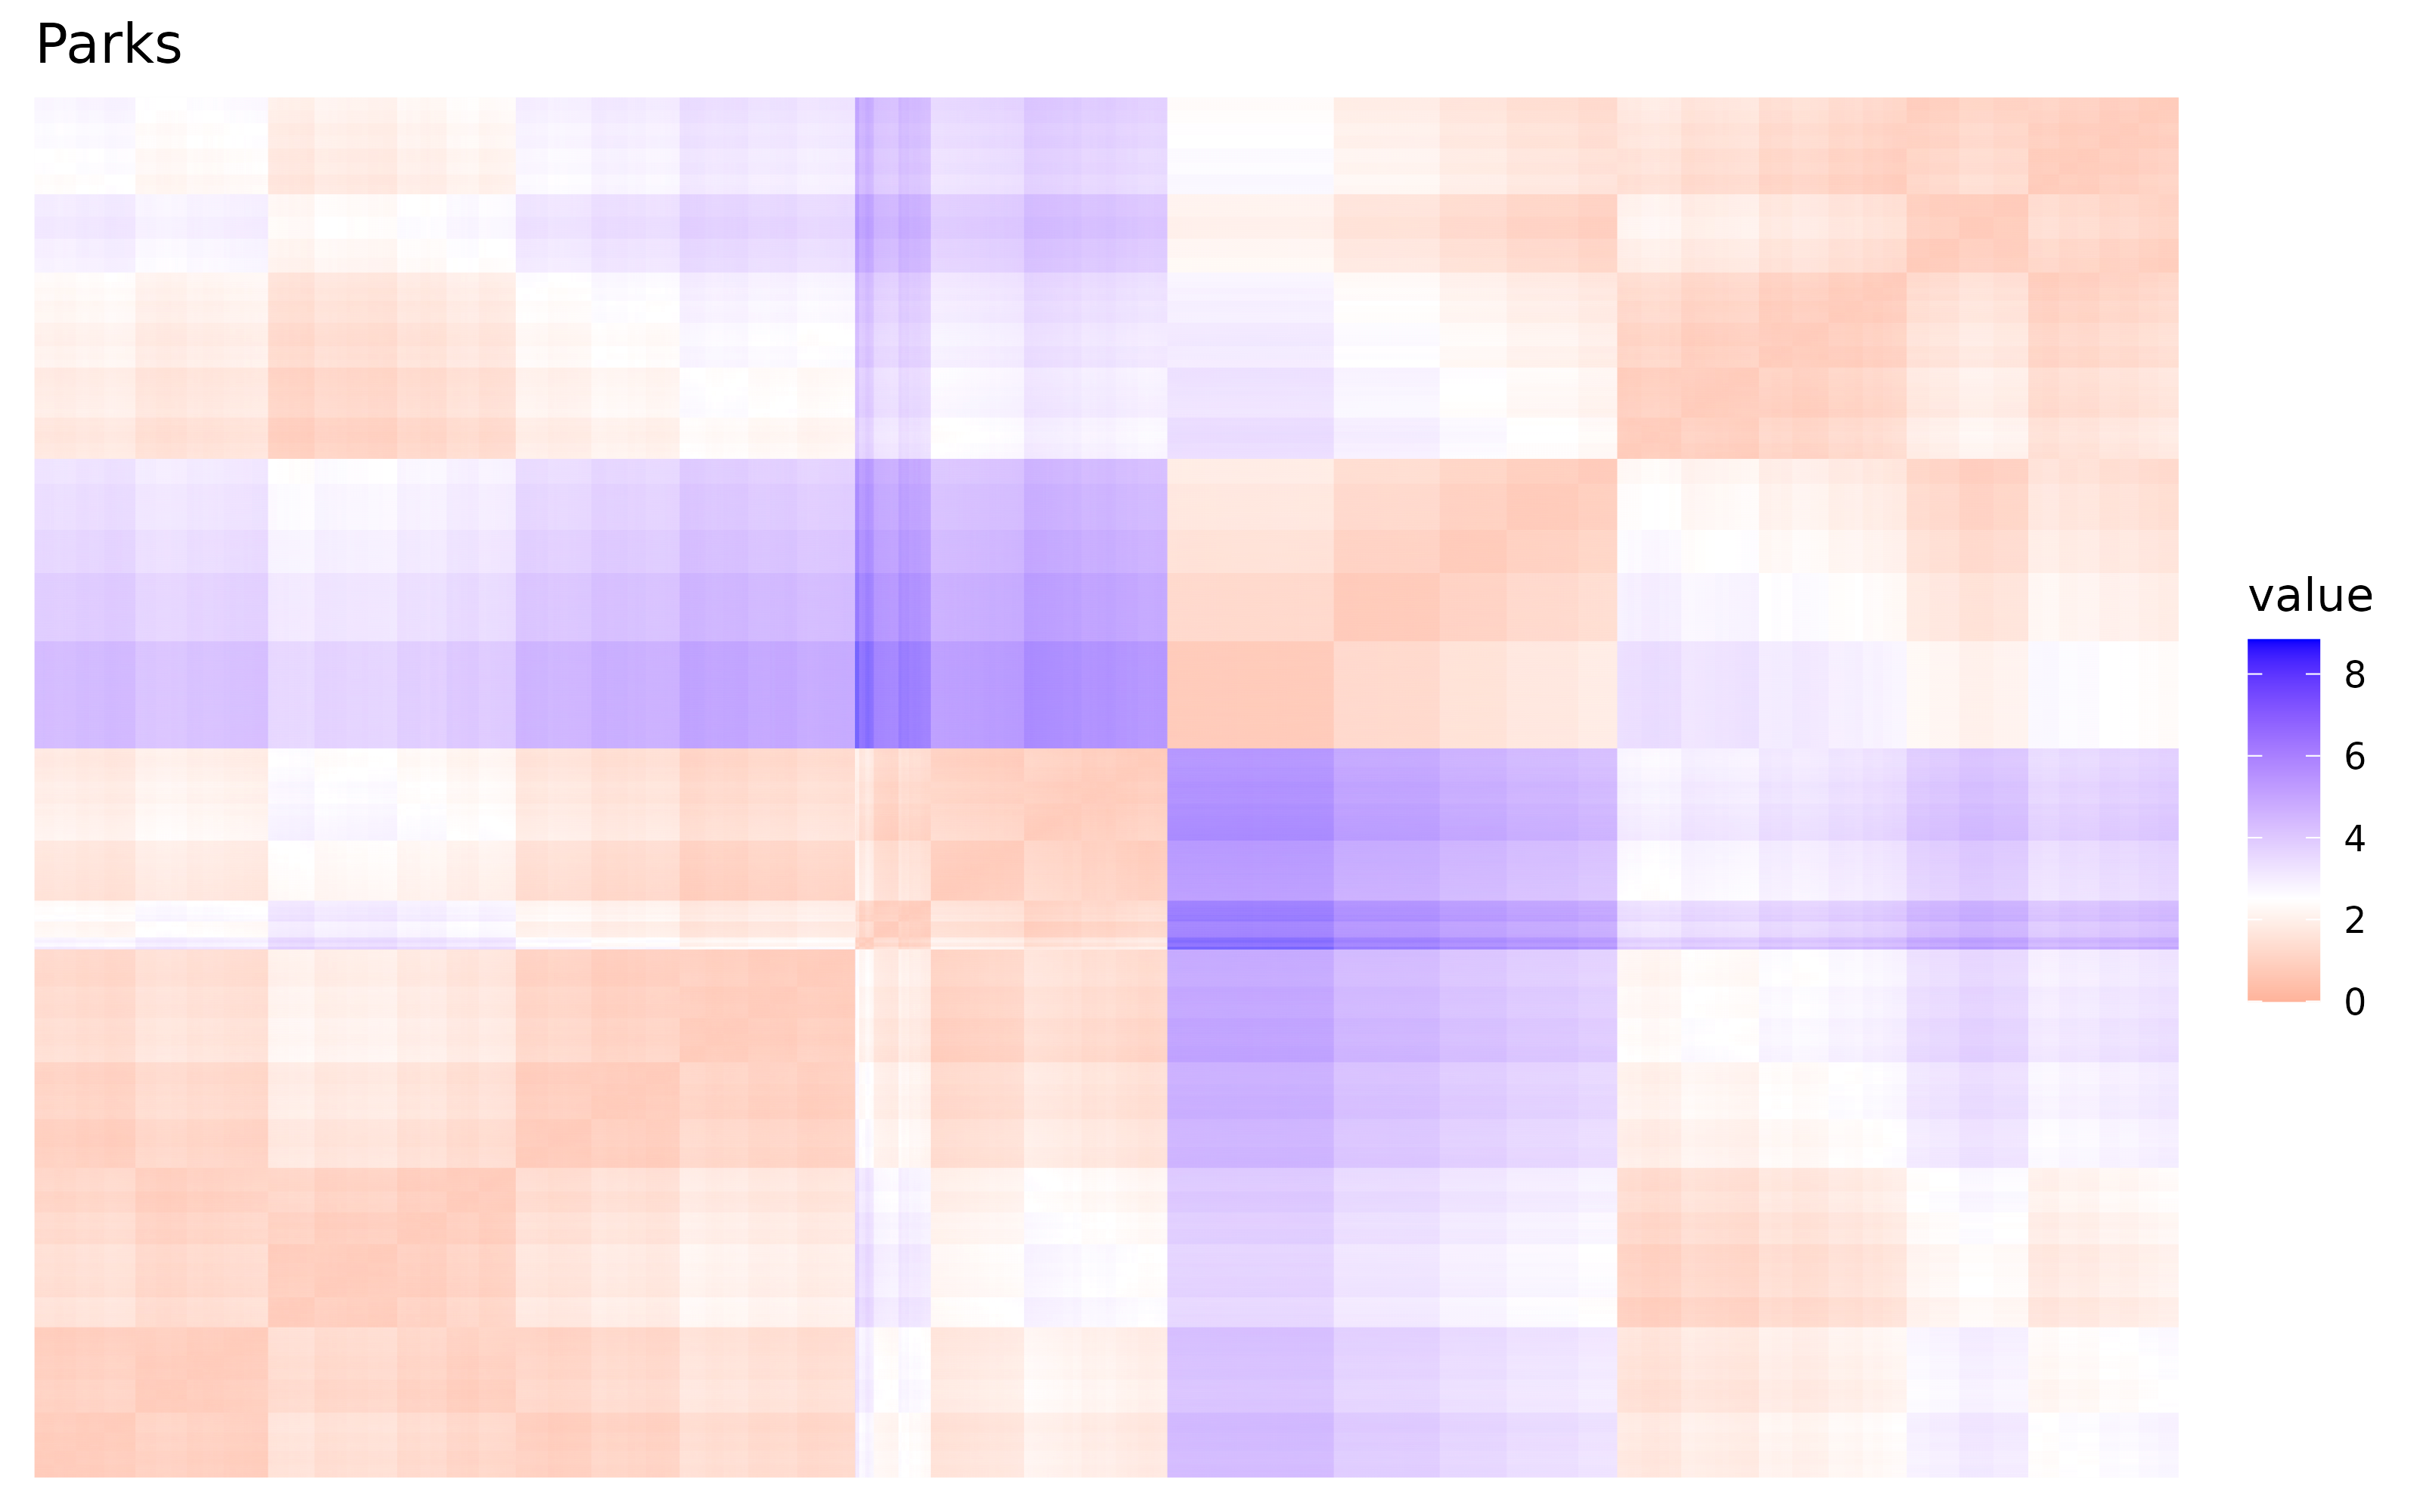
\includegraphics[width=\textwidth]{./vat/parks_vat_log.png}
\caption[Parks VAT plot]{VAT plot for the log-transformed parks amenity.}\label{parksvat}
\end{figure}










\begin{figure}[H]
\centering
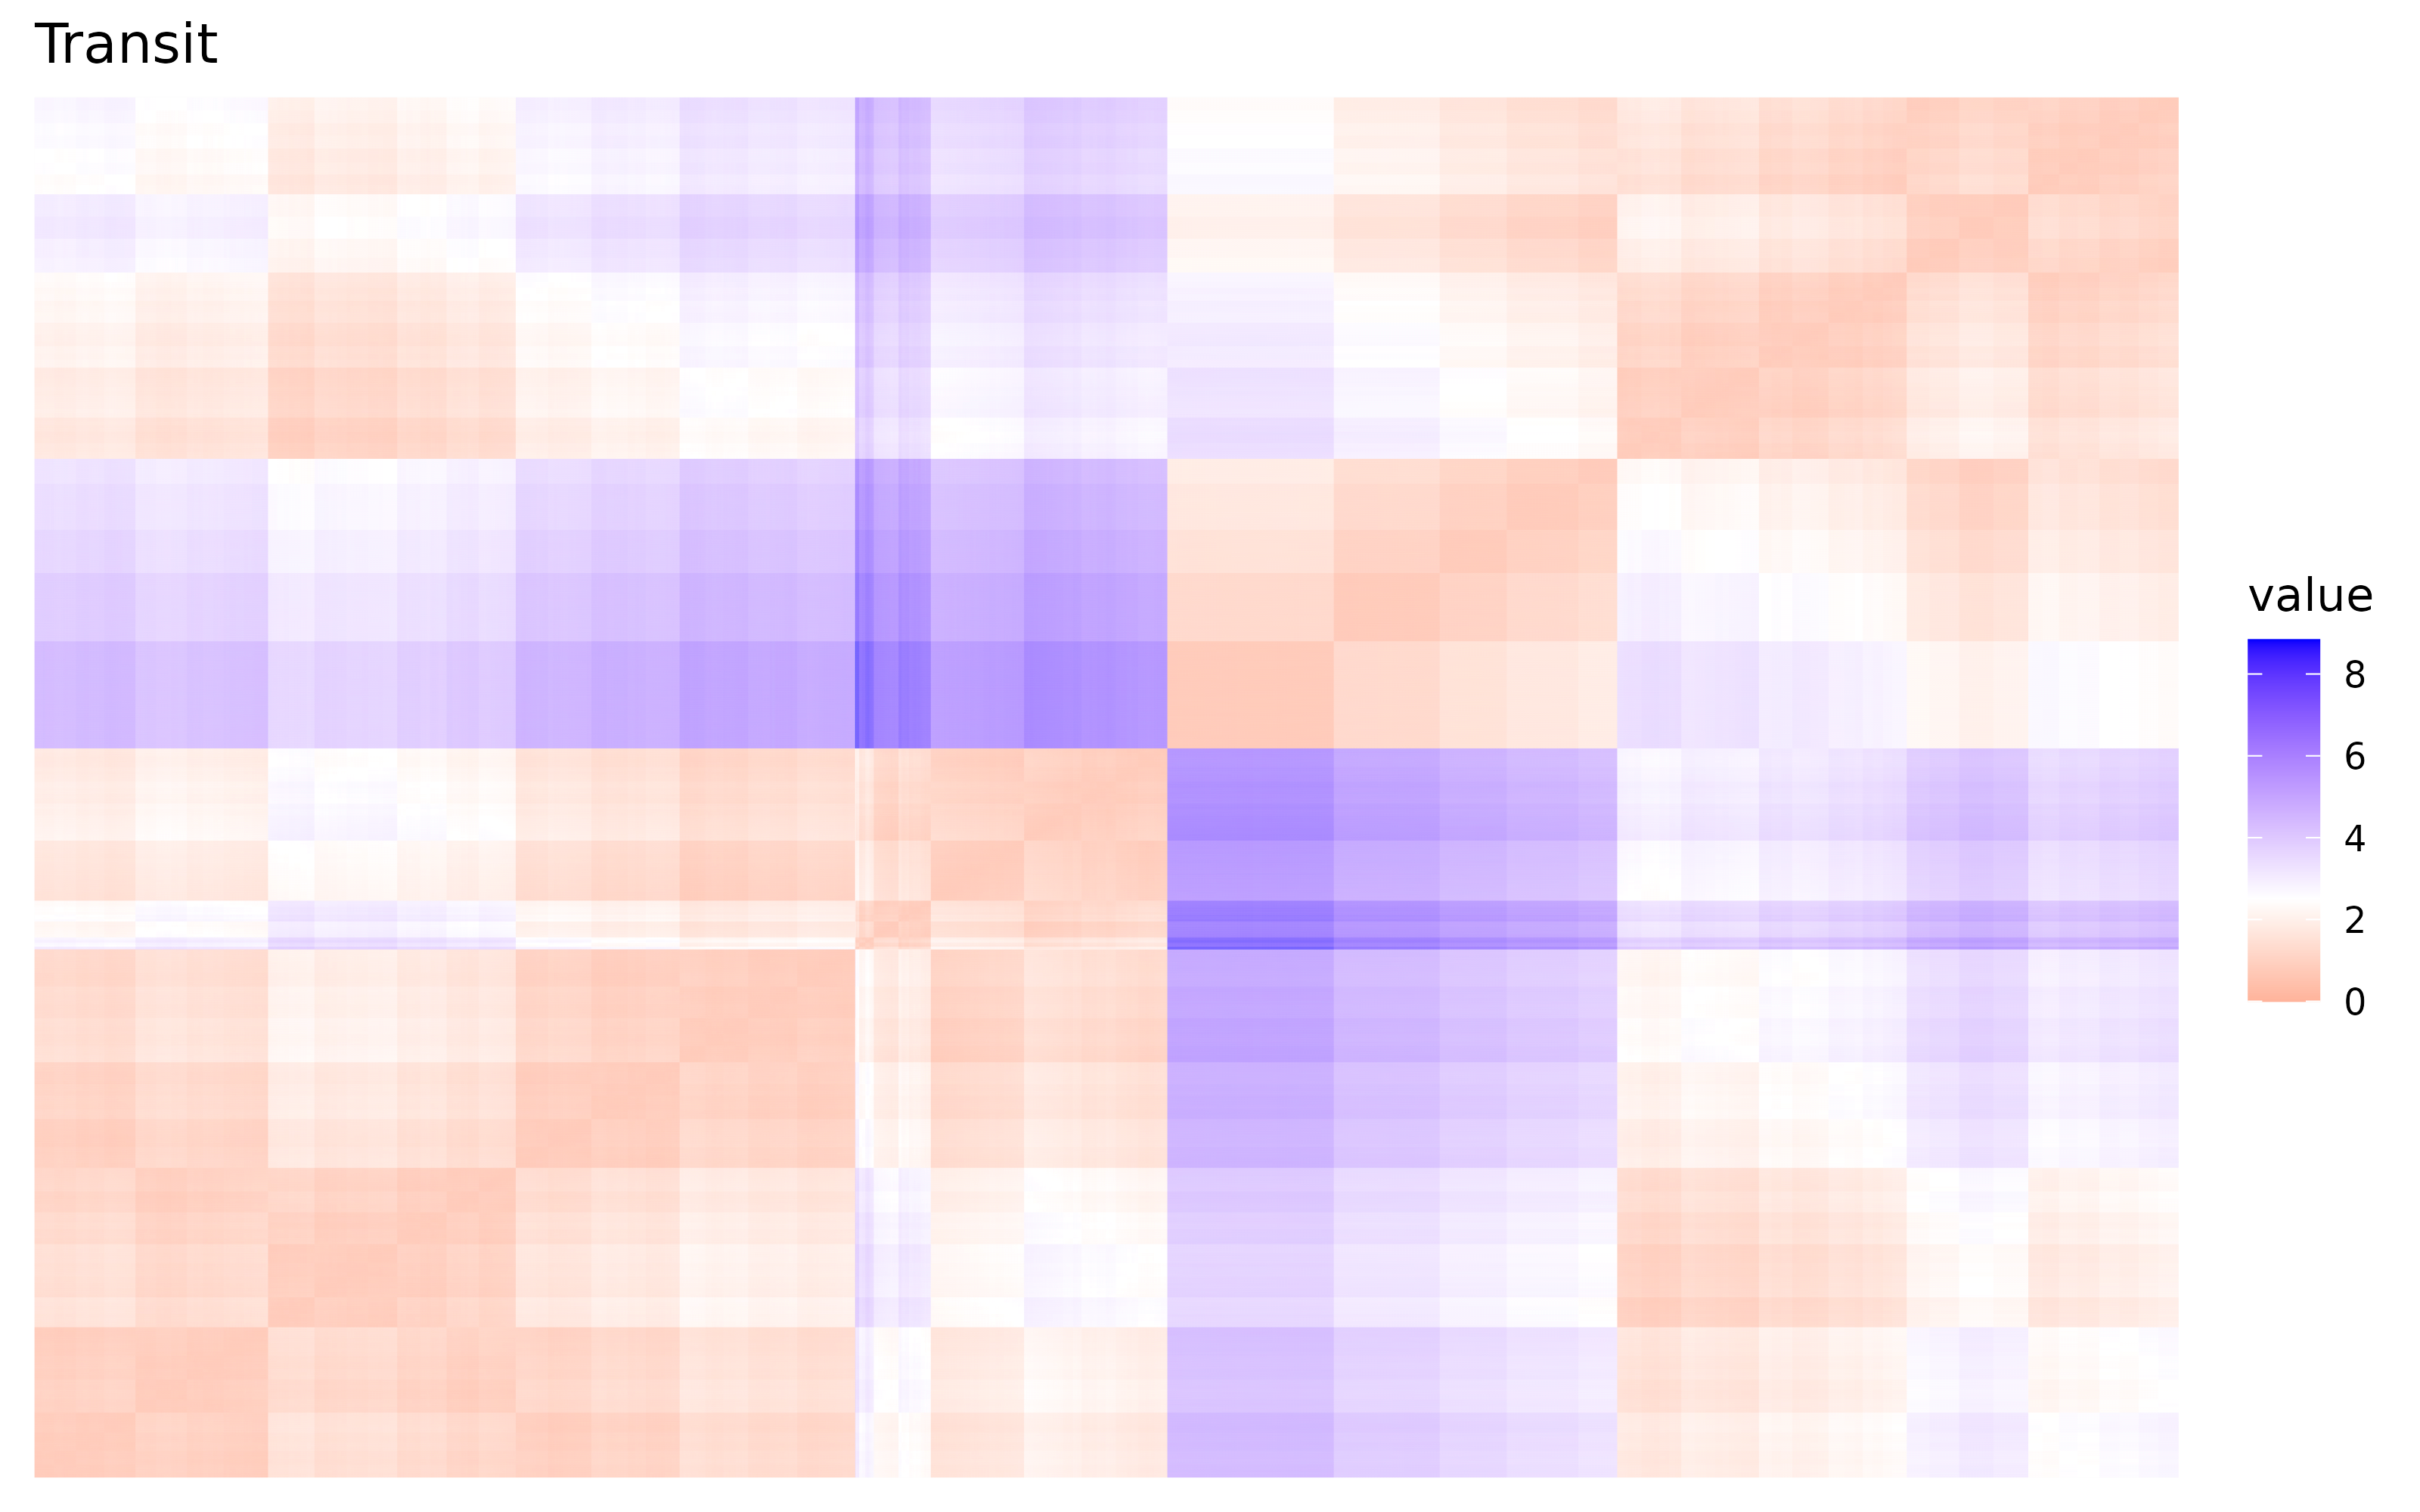
\includegraphics[width=\textwidth]{./vat/transit_vat_log.png}
\caption[Transit VAT plot]{VAT plot for the log-transformed transit amenity.}\label{transitvat}
\end{figure}









\begin{figure}[H]
\centering
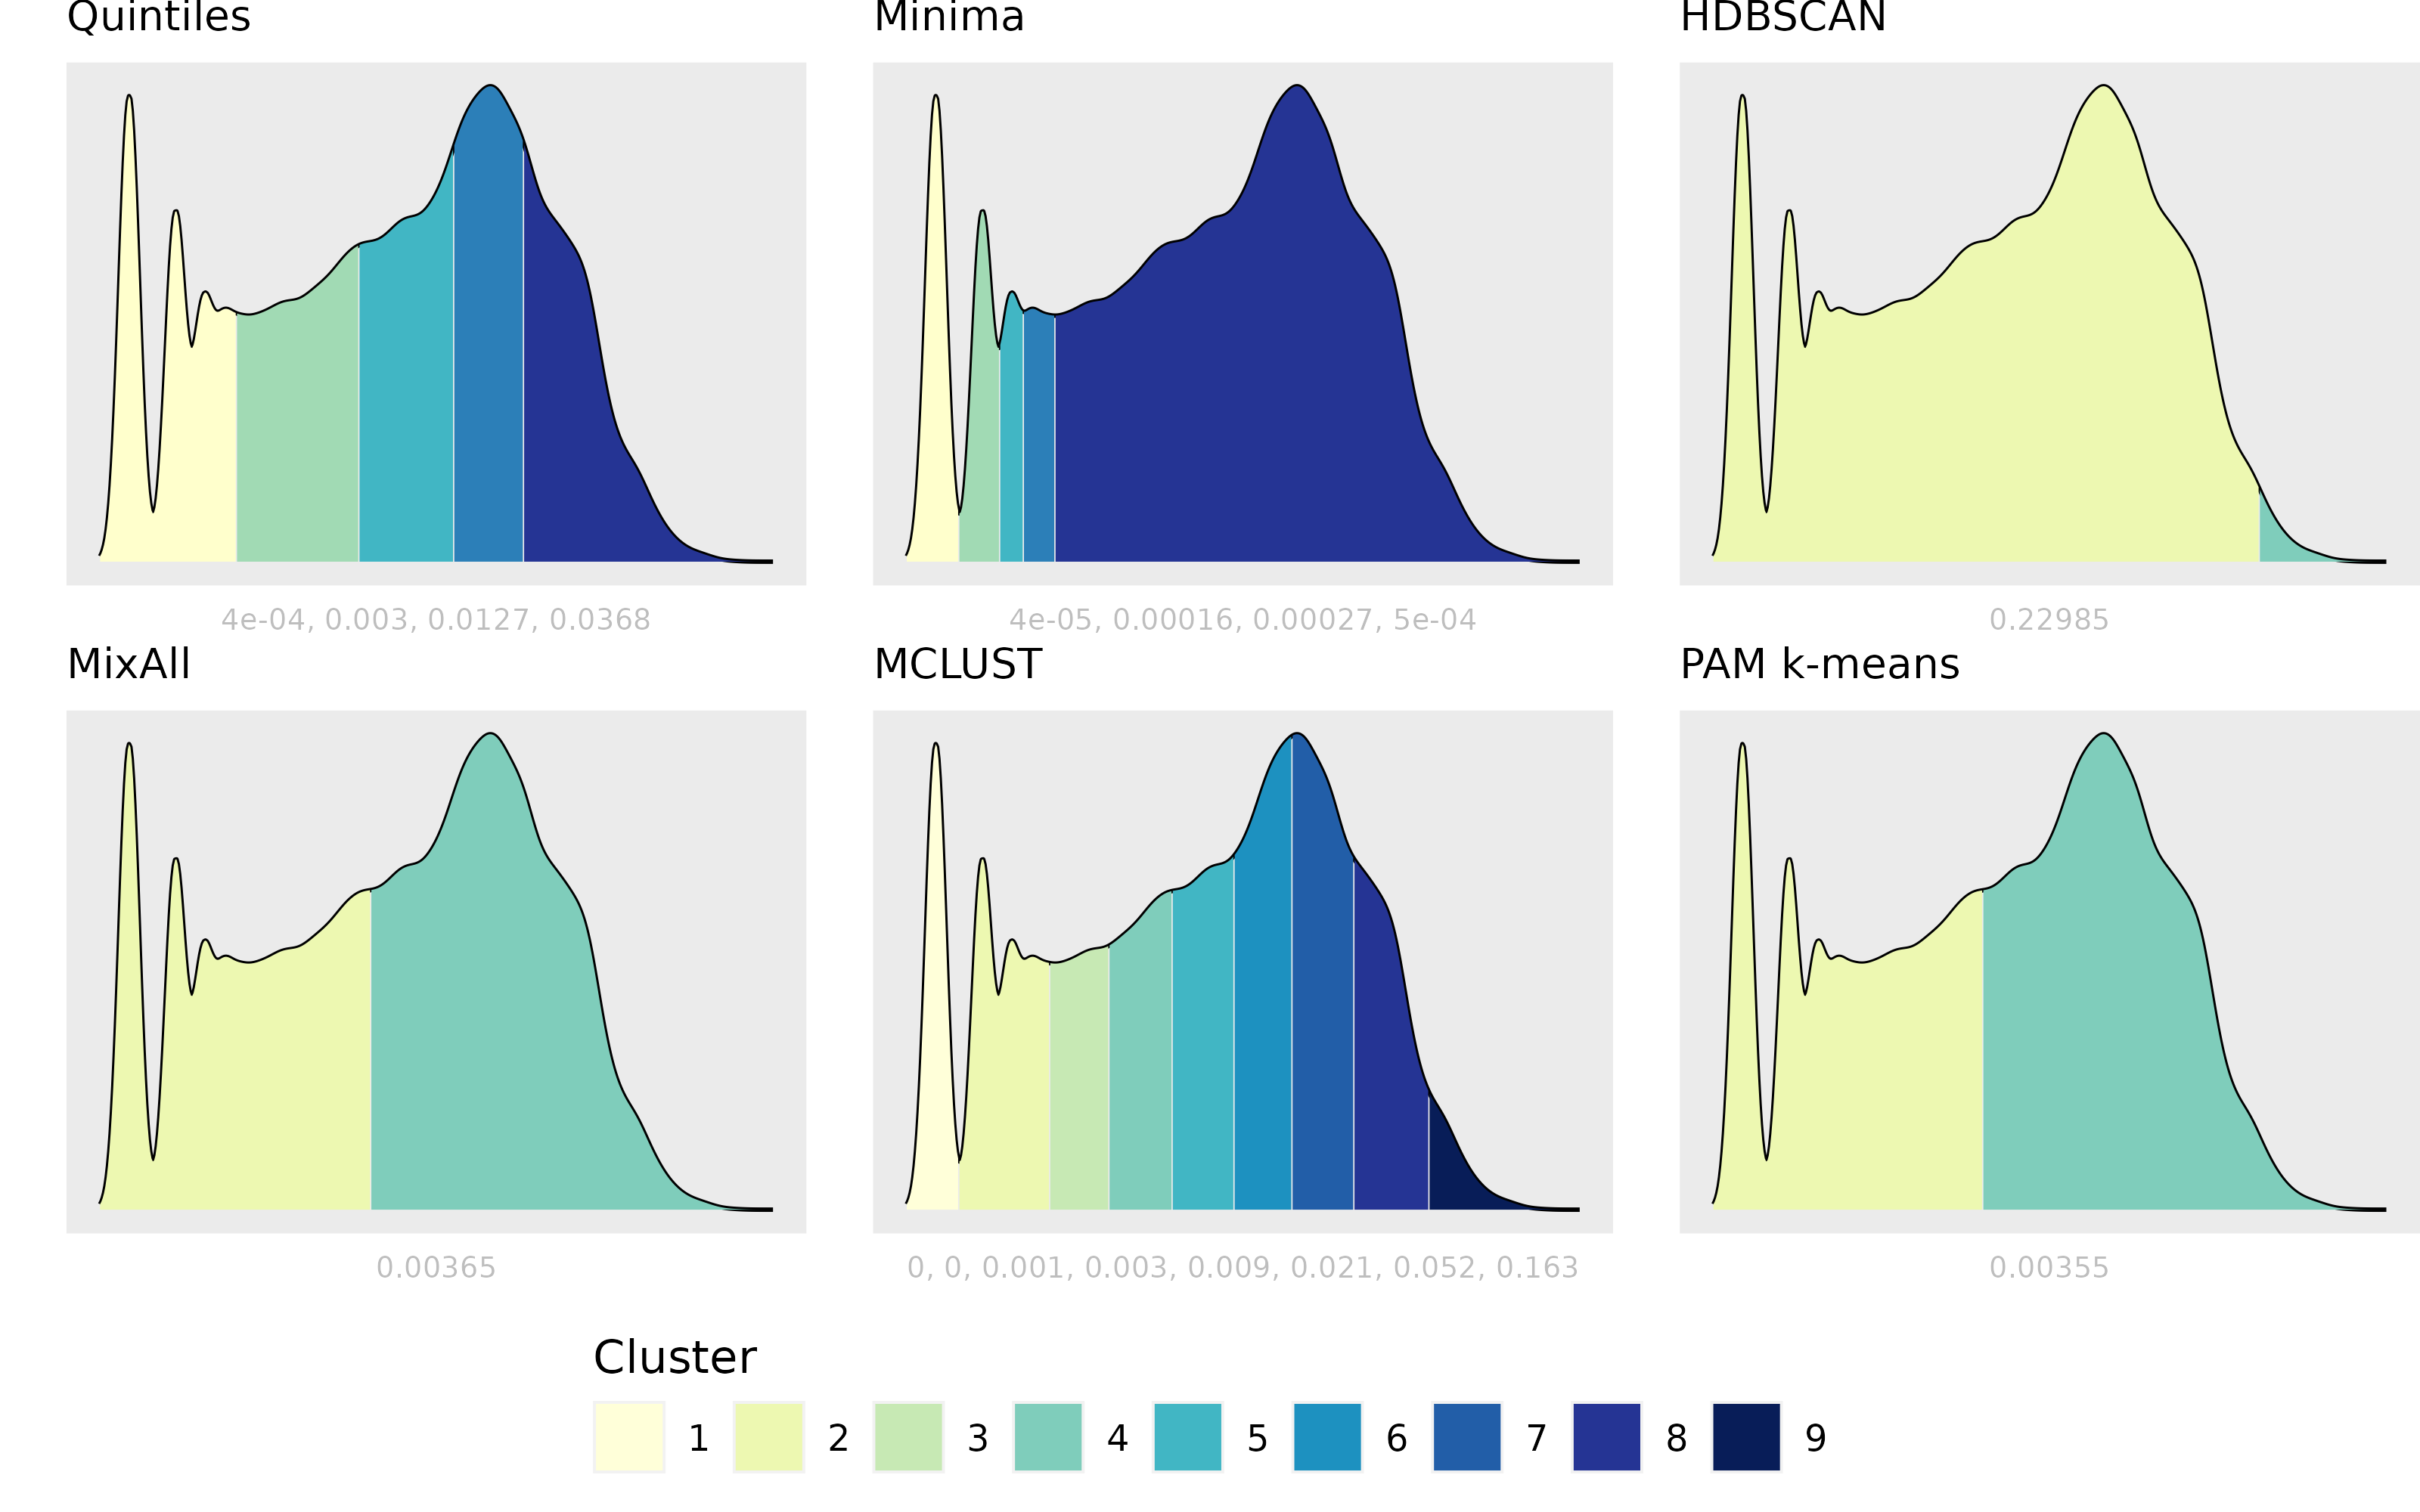
\includegraphics[width=\textwidth]{./cutoffs/by_amenity/Employment_cutoffs.png}
\caption[Employment cutoffs]{Cut-offs values shown on the log-transformed density plots for all clustering approaches employment amenity.}\label{employmentcutoffs}
\end{figure}









\begin{figure}[H]
\centering
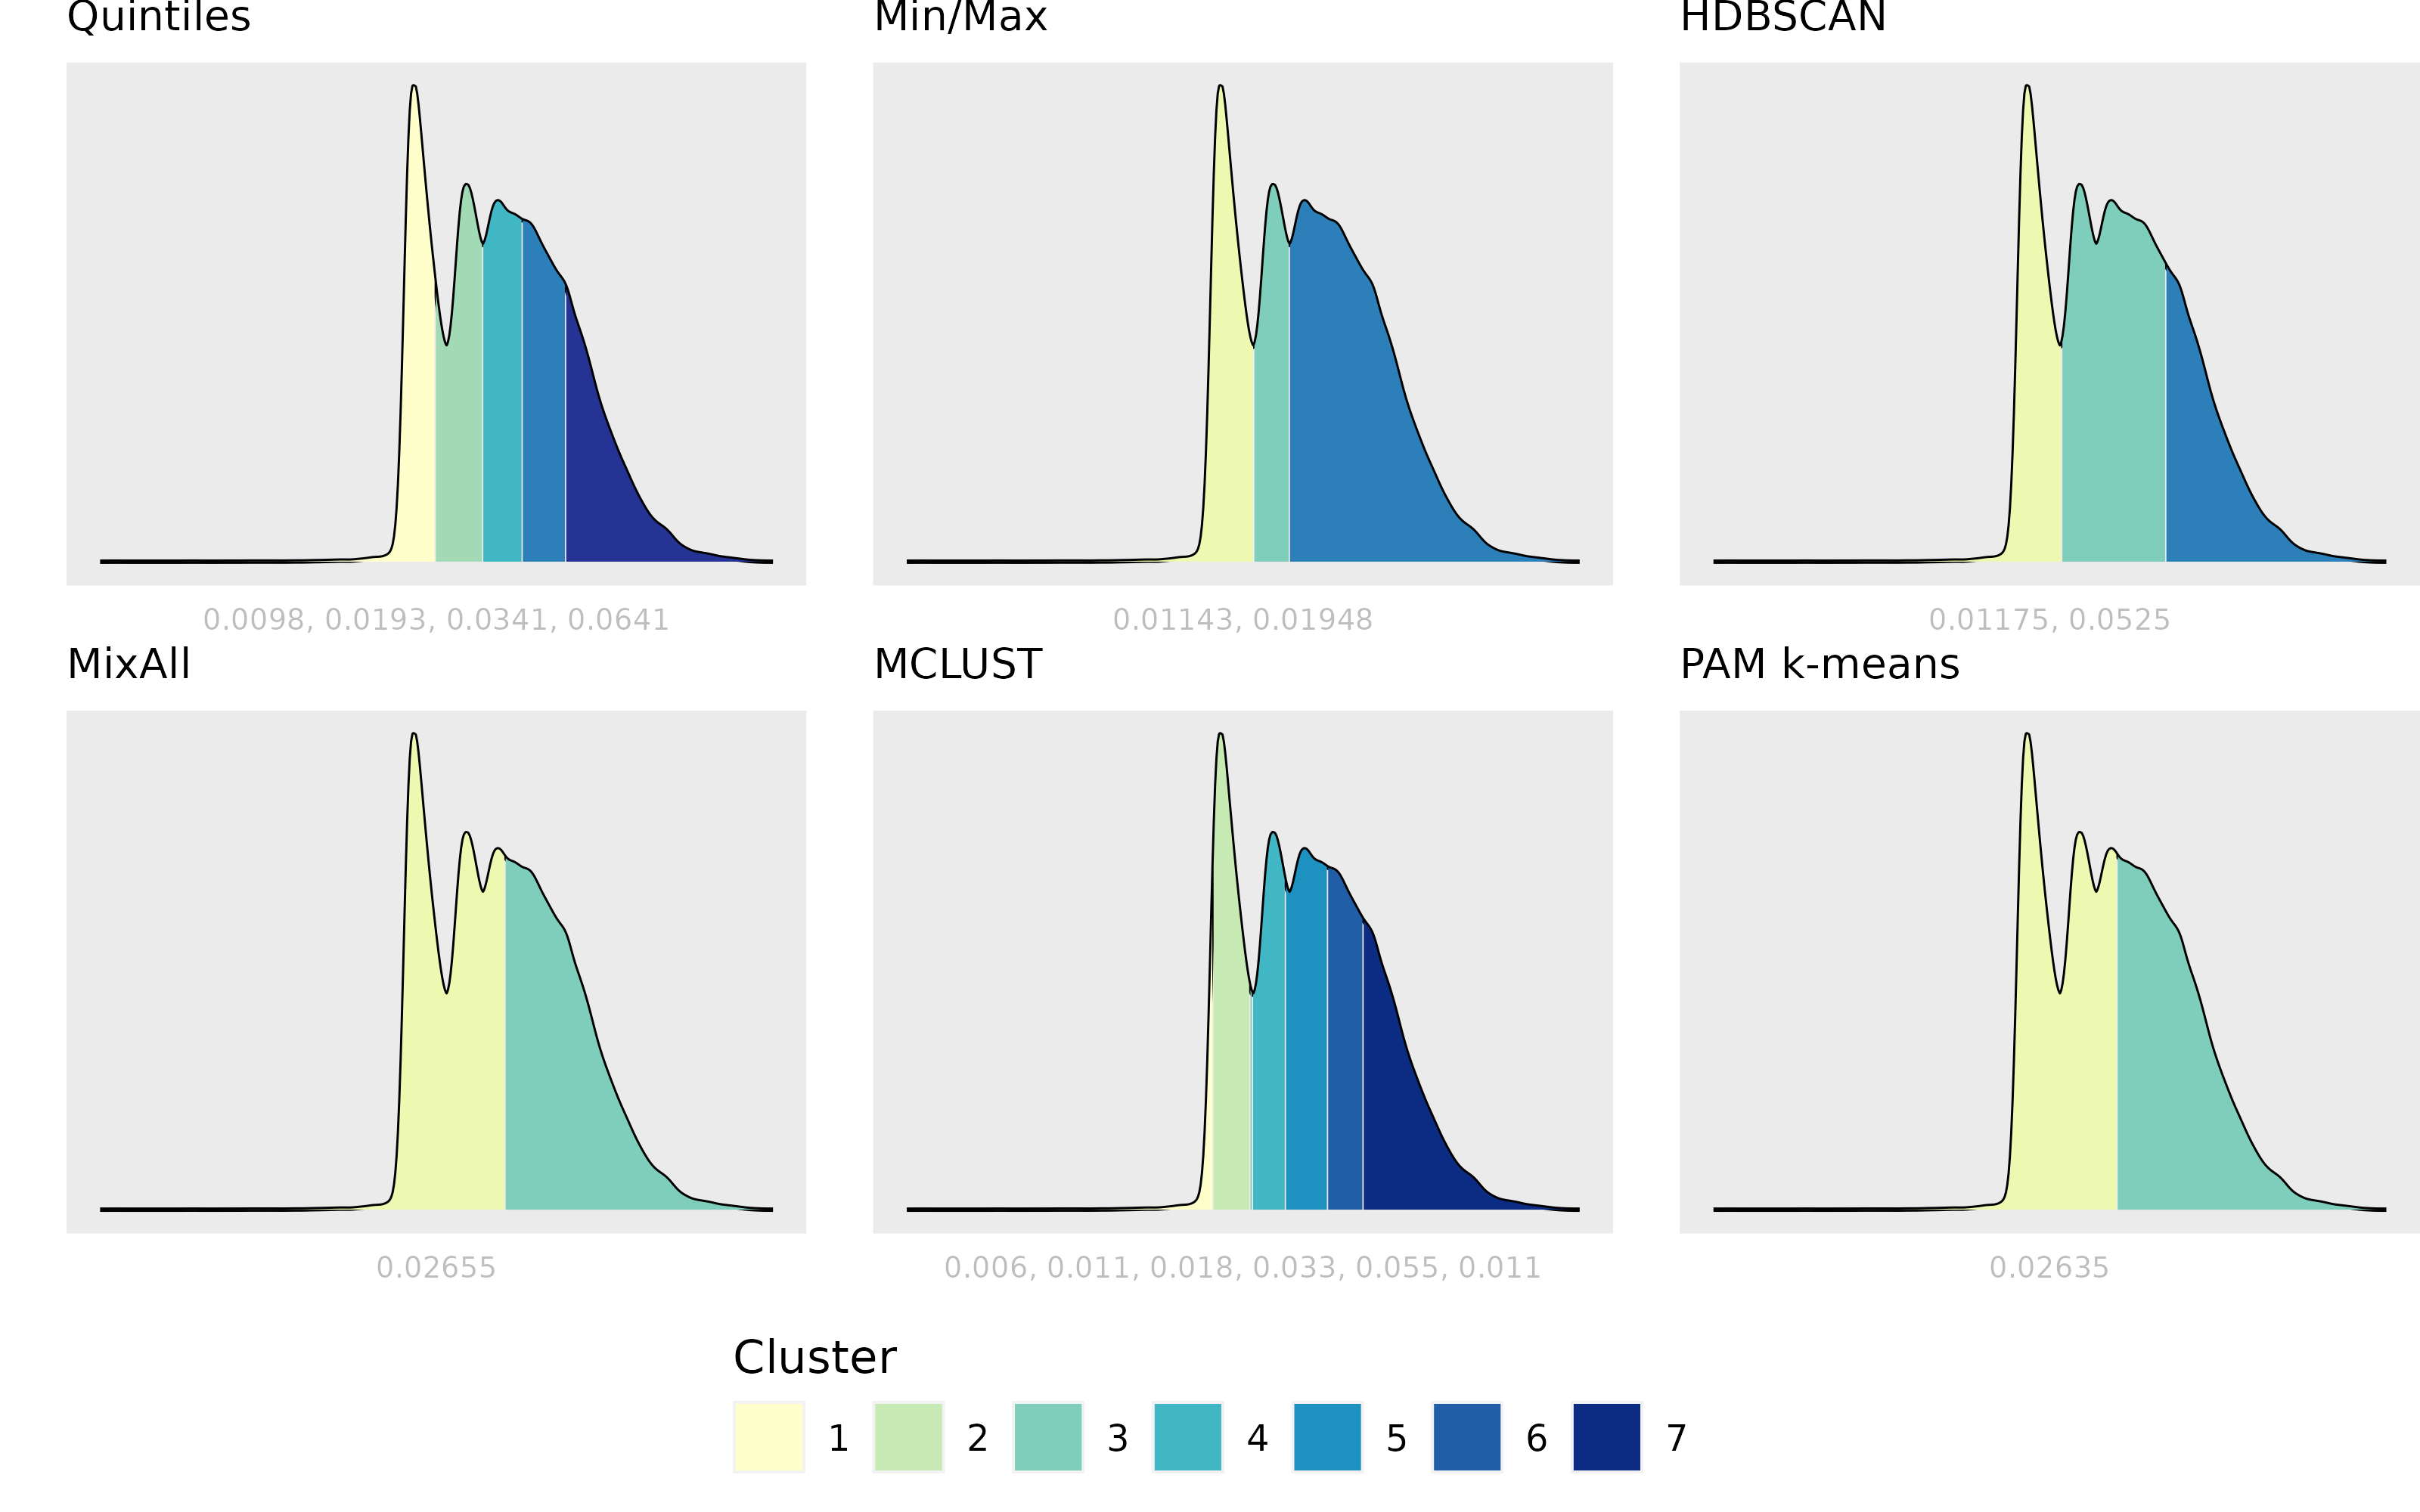
\includegraphics[width=\textwidth]{./cutoffs/by_amenity/Pharmacy_cutoffs.png}
\caption[Pharmacy cutoffs]{Cut-offs values shown on the log-transformed density plots for all clustering approaches pharmacy amenity.}\label{pharmacycutoffs}
\end{figure}










\begin{figure}[H]
\centering
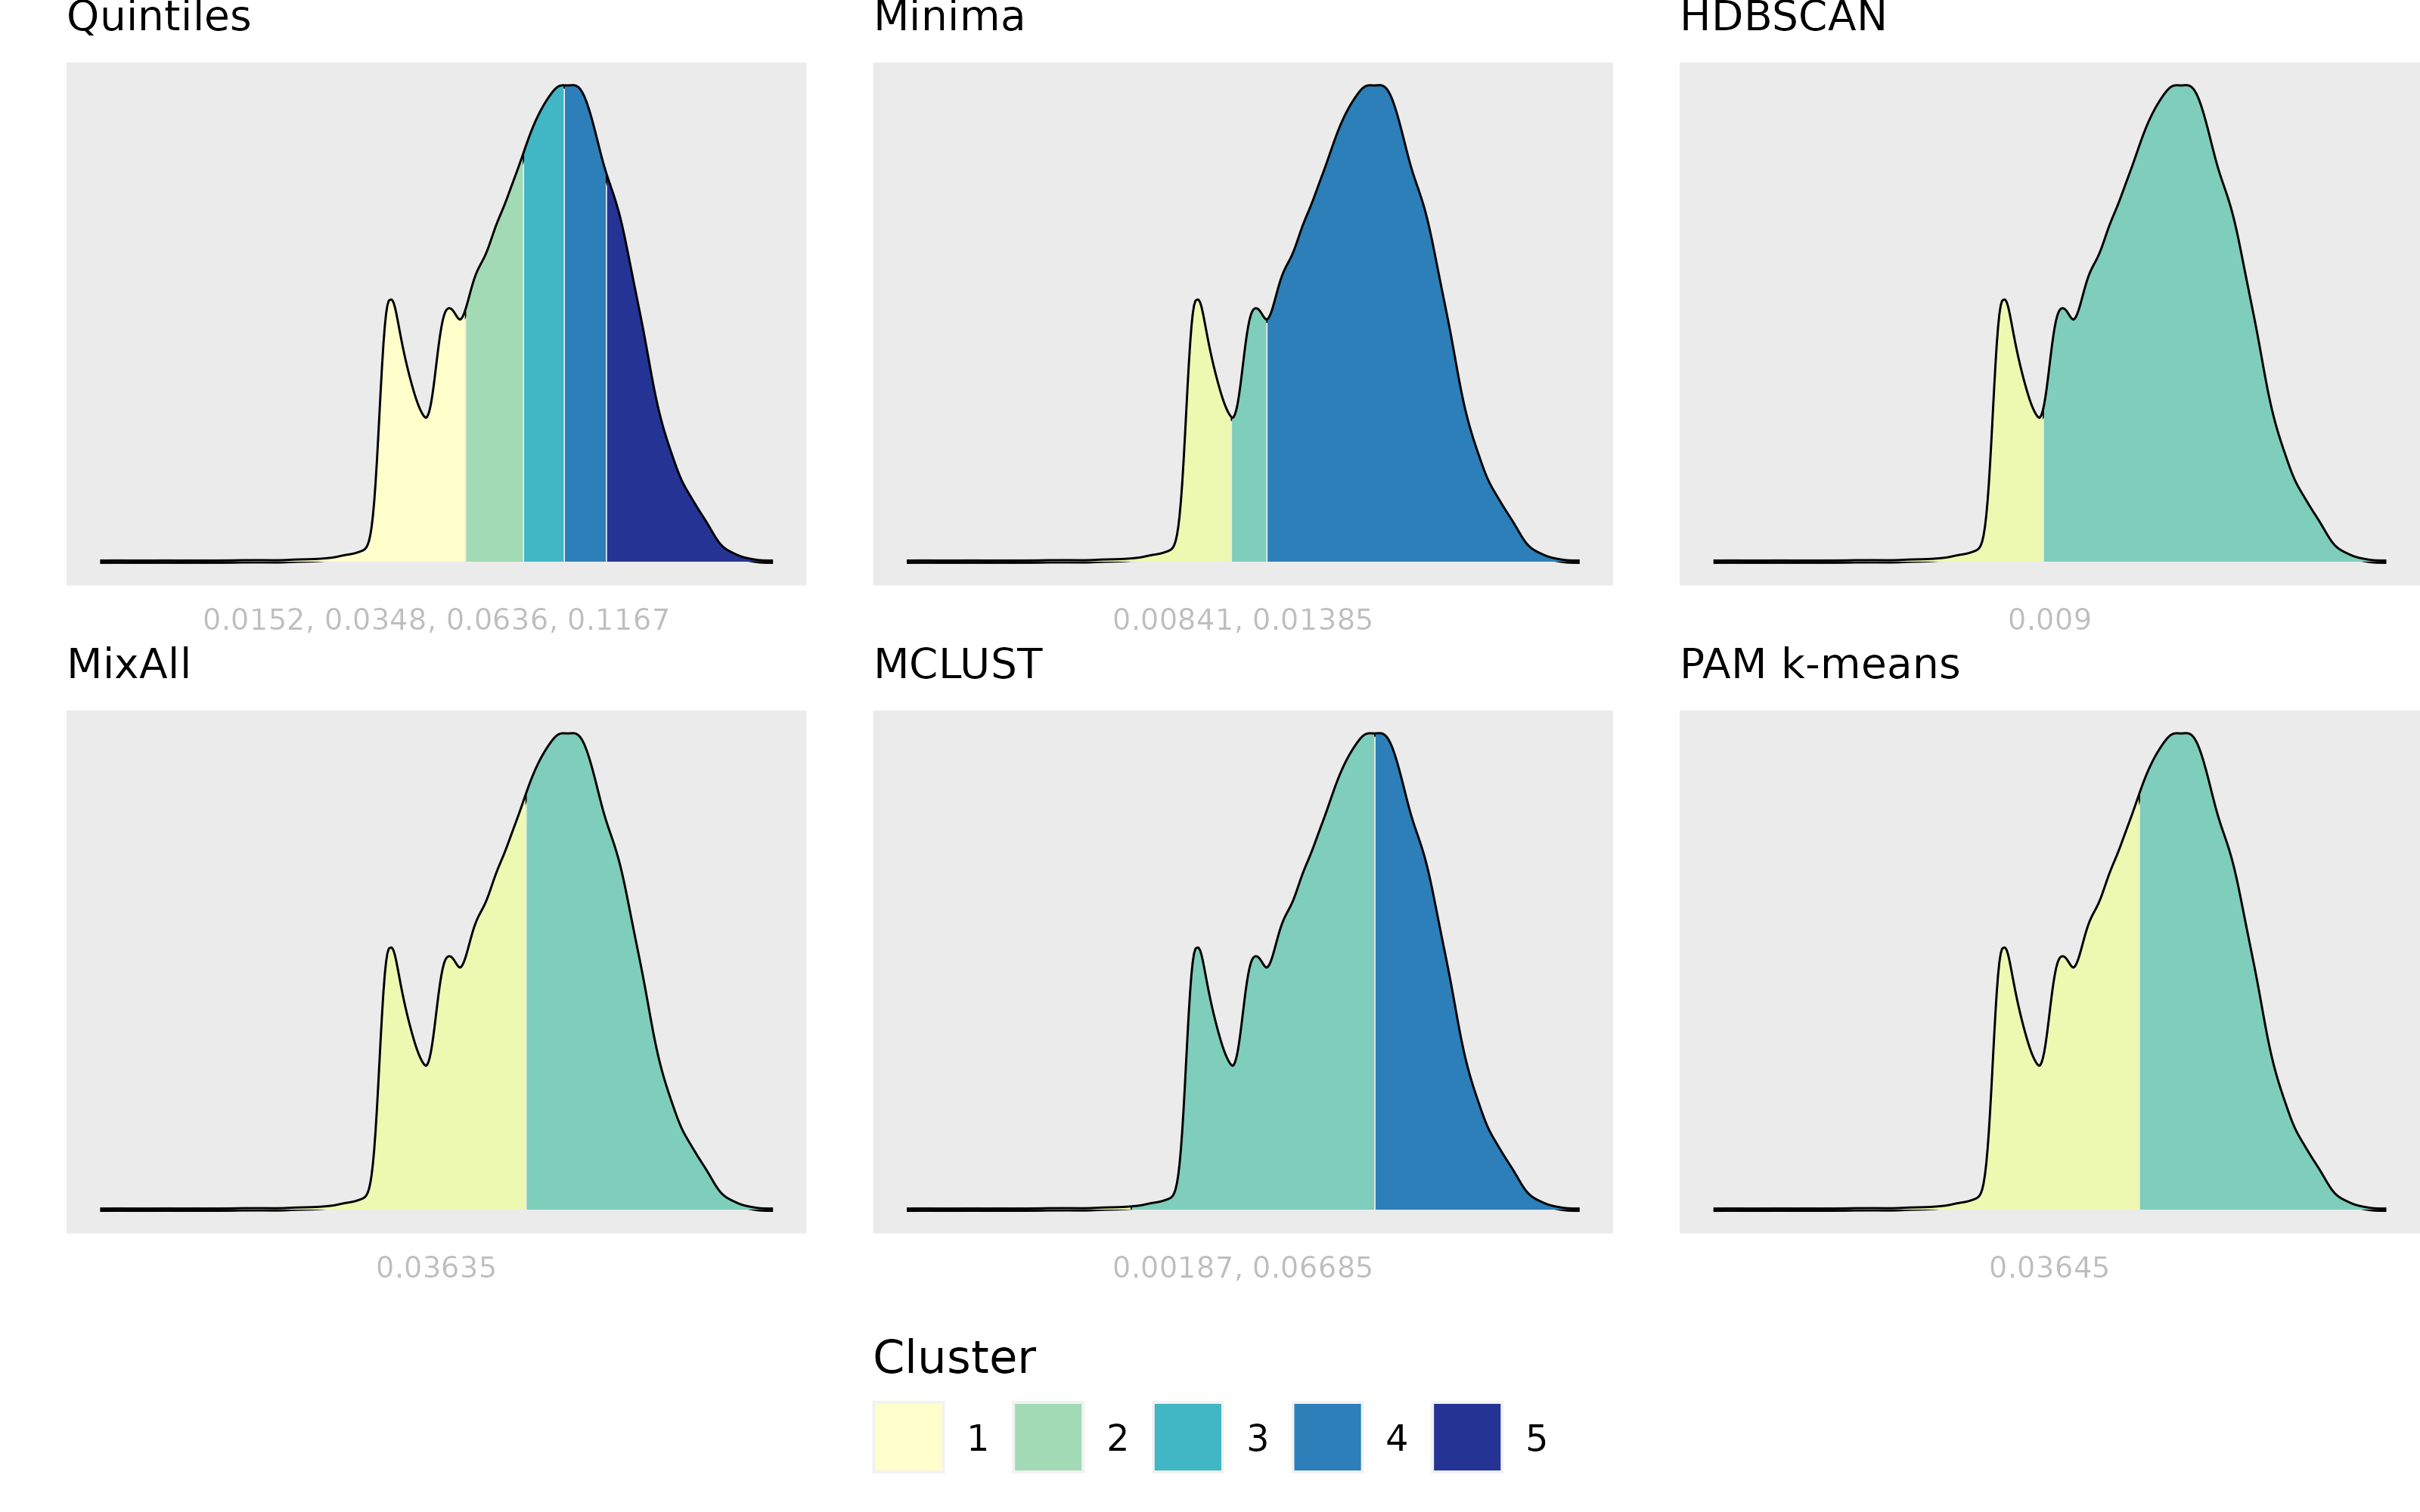
\includegraphics[width=\textwidth]{./cutoffs/by_amenity/Child care_cutoffs.png}
\caption[Child care cutoffs]{Cut-offs values shown on the log-transformed density plots for all clustering approaches child care amenity.}\label{childcarecutoffs}
\end{figure}










\begin{figure}[H]
\centering
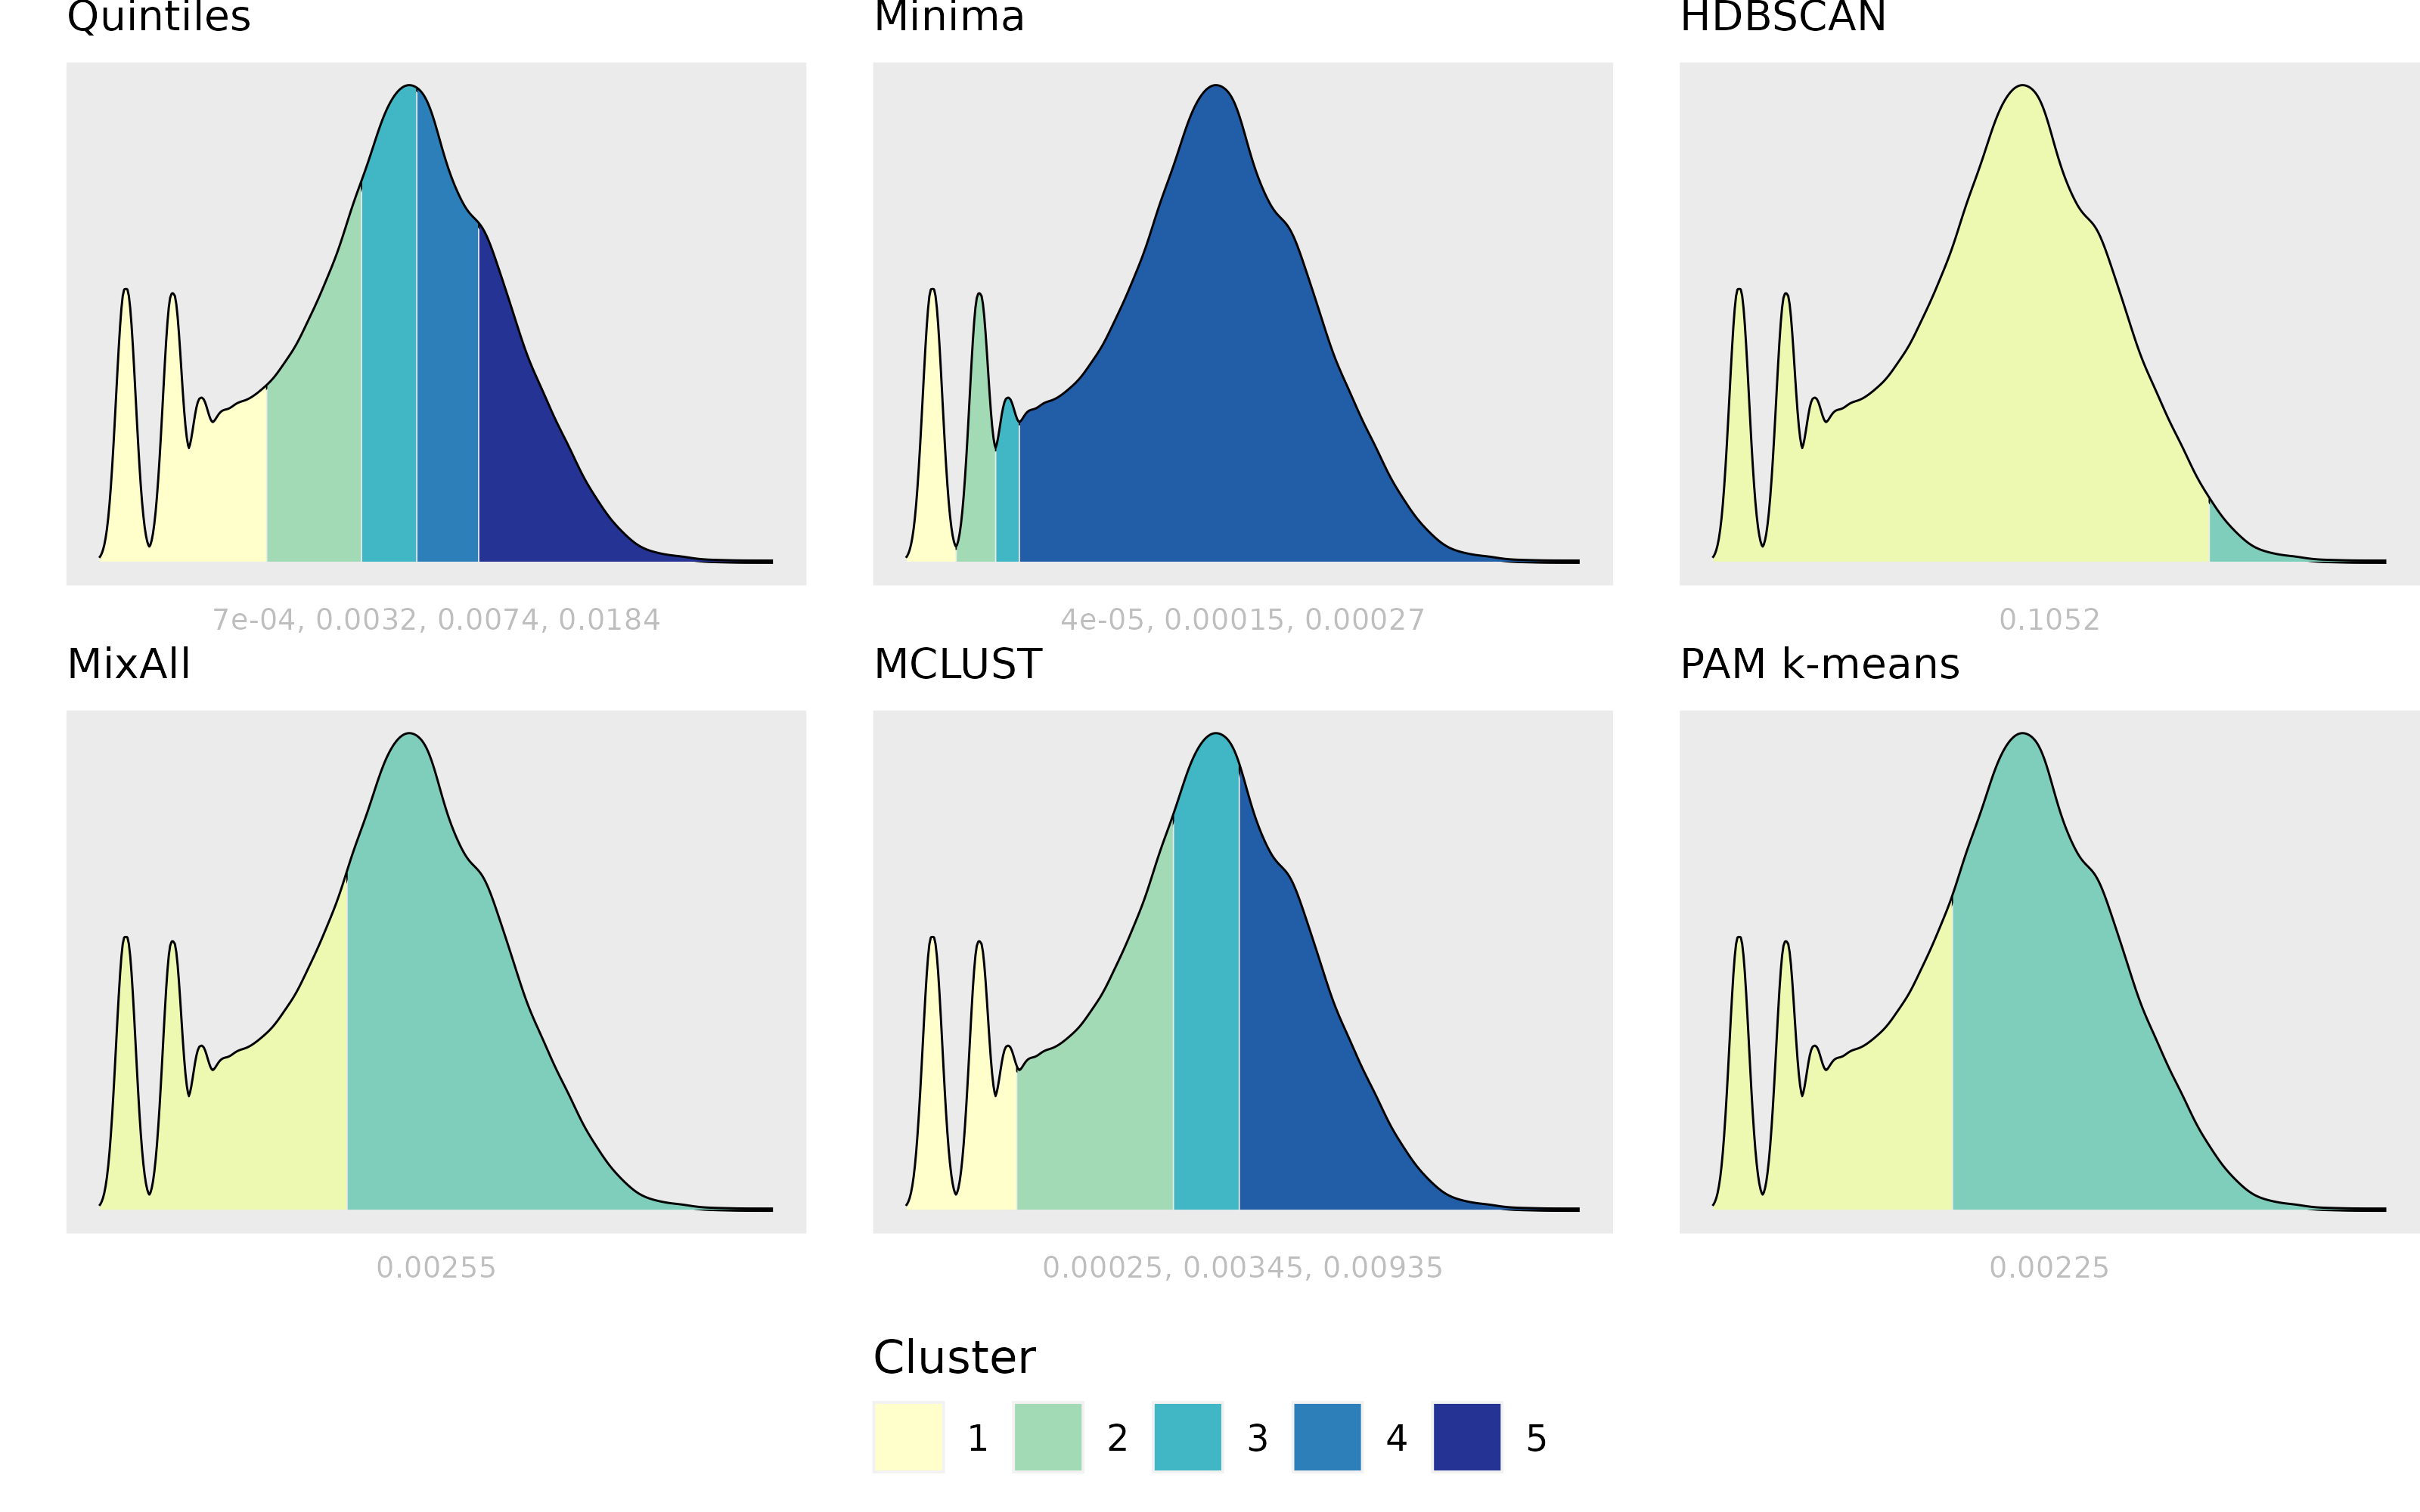
\includegraphics[width=\textwidth]{./cutoffs/by_amenity/Health care_cutoffs.png}
\caption[Health care cutoffs]{Cut-offs values shown on the log-transformed density plots for all clustering approaches health care amenity.}\label{healthcarecutoffs}
\end{figure}










\begin{figure}[H]
\centering
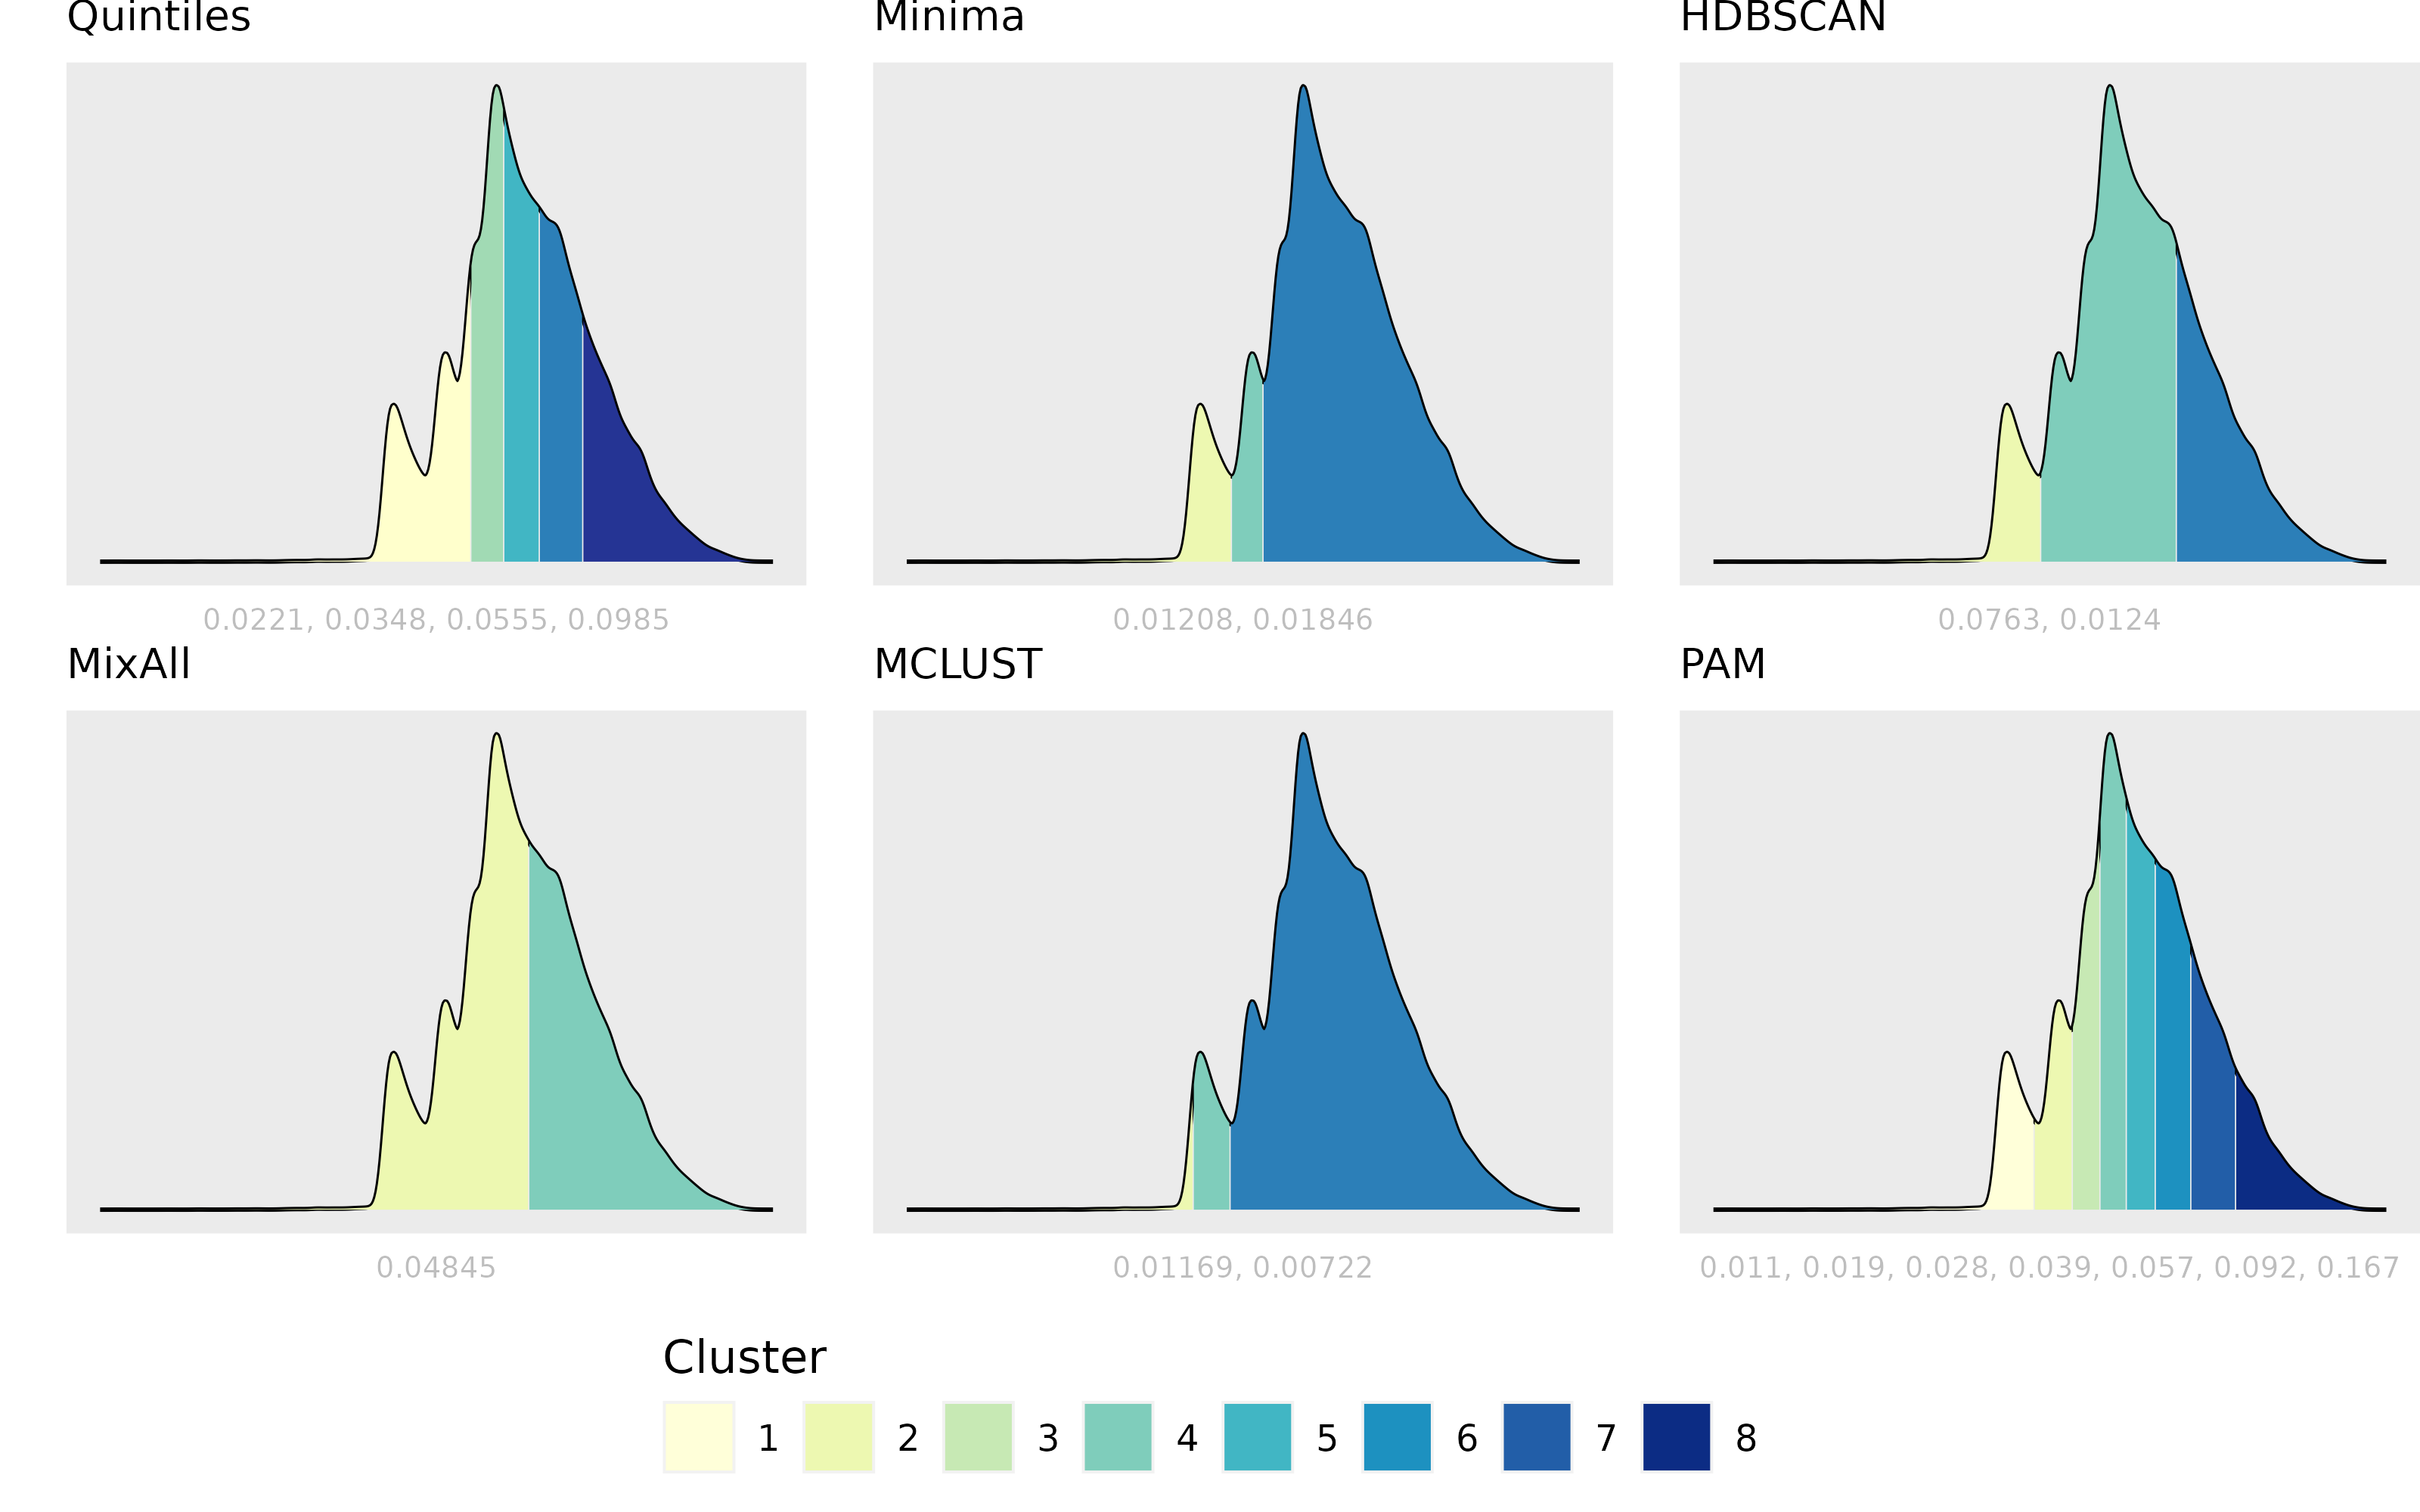
\includegraphics[width=\textwidth]{./cutoffs/by_amenity/Grocery_cutoffs.png}
\caption[Grocery cutoffs]{Cut-offs values shown on the log-transformed density plots for all clustering approaches grocery amenity.}\label{grocerycutoffs}
\end{figure}










\begin{figure}[H]
\centering
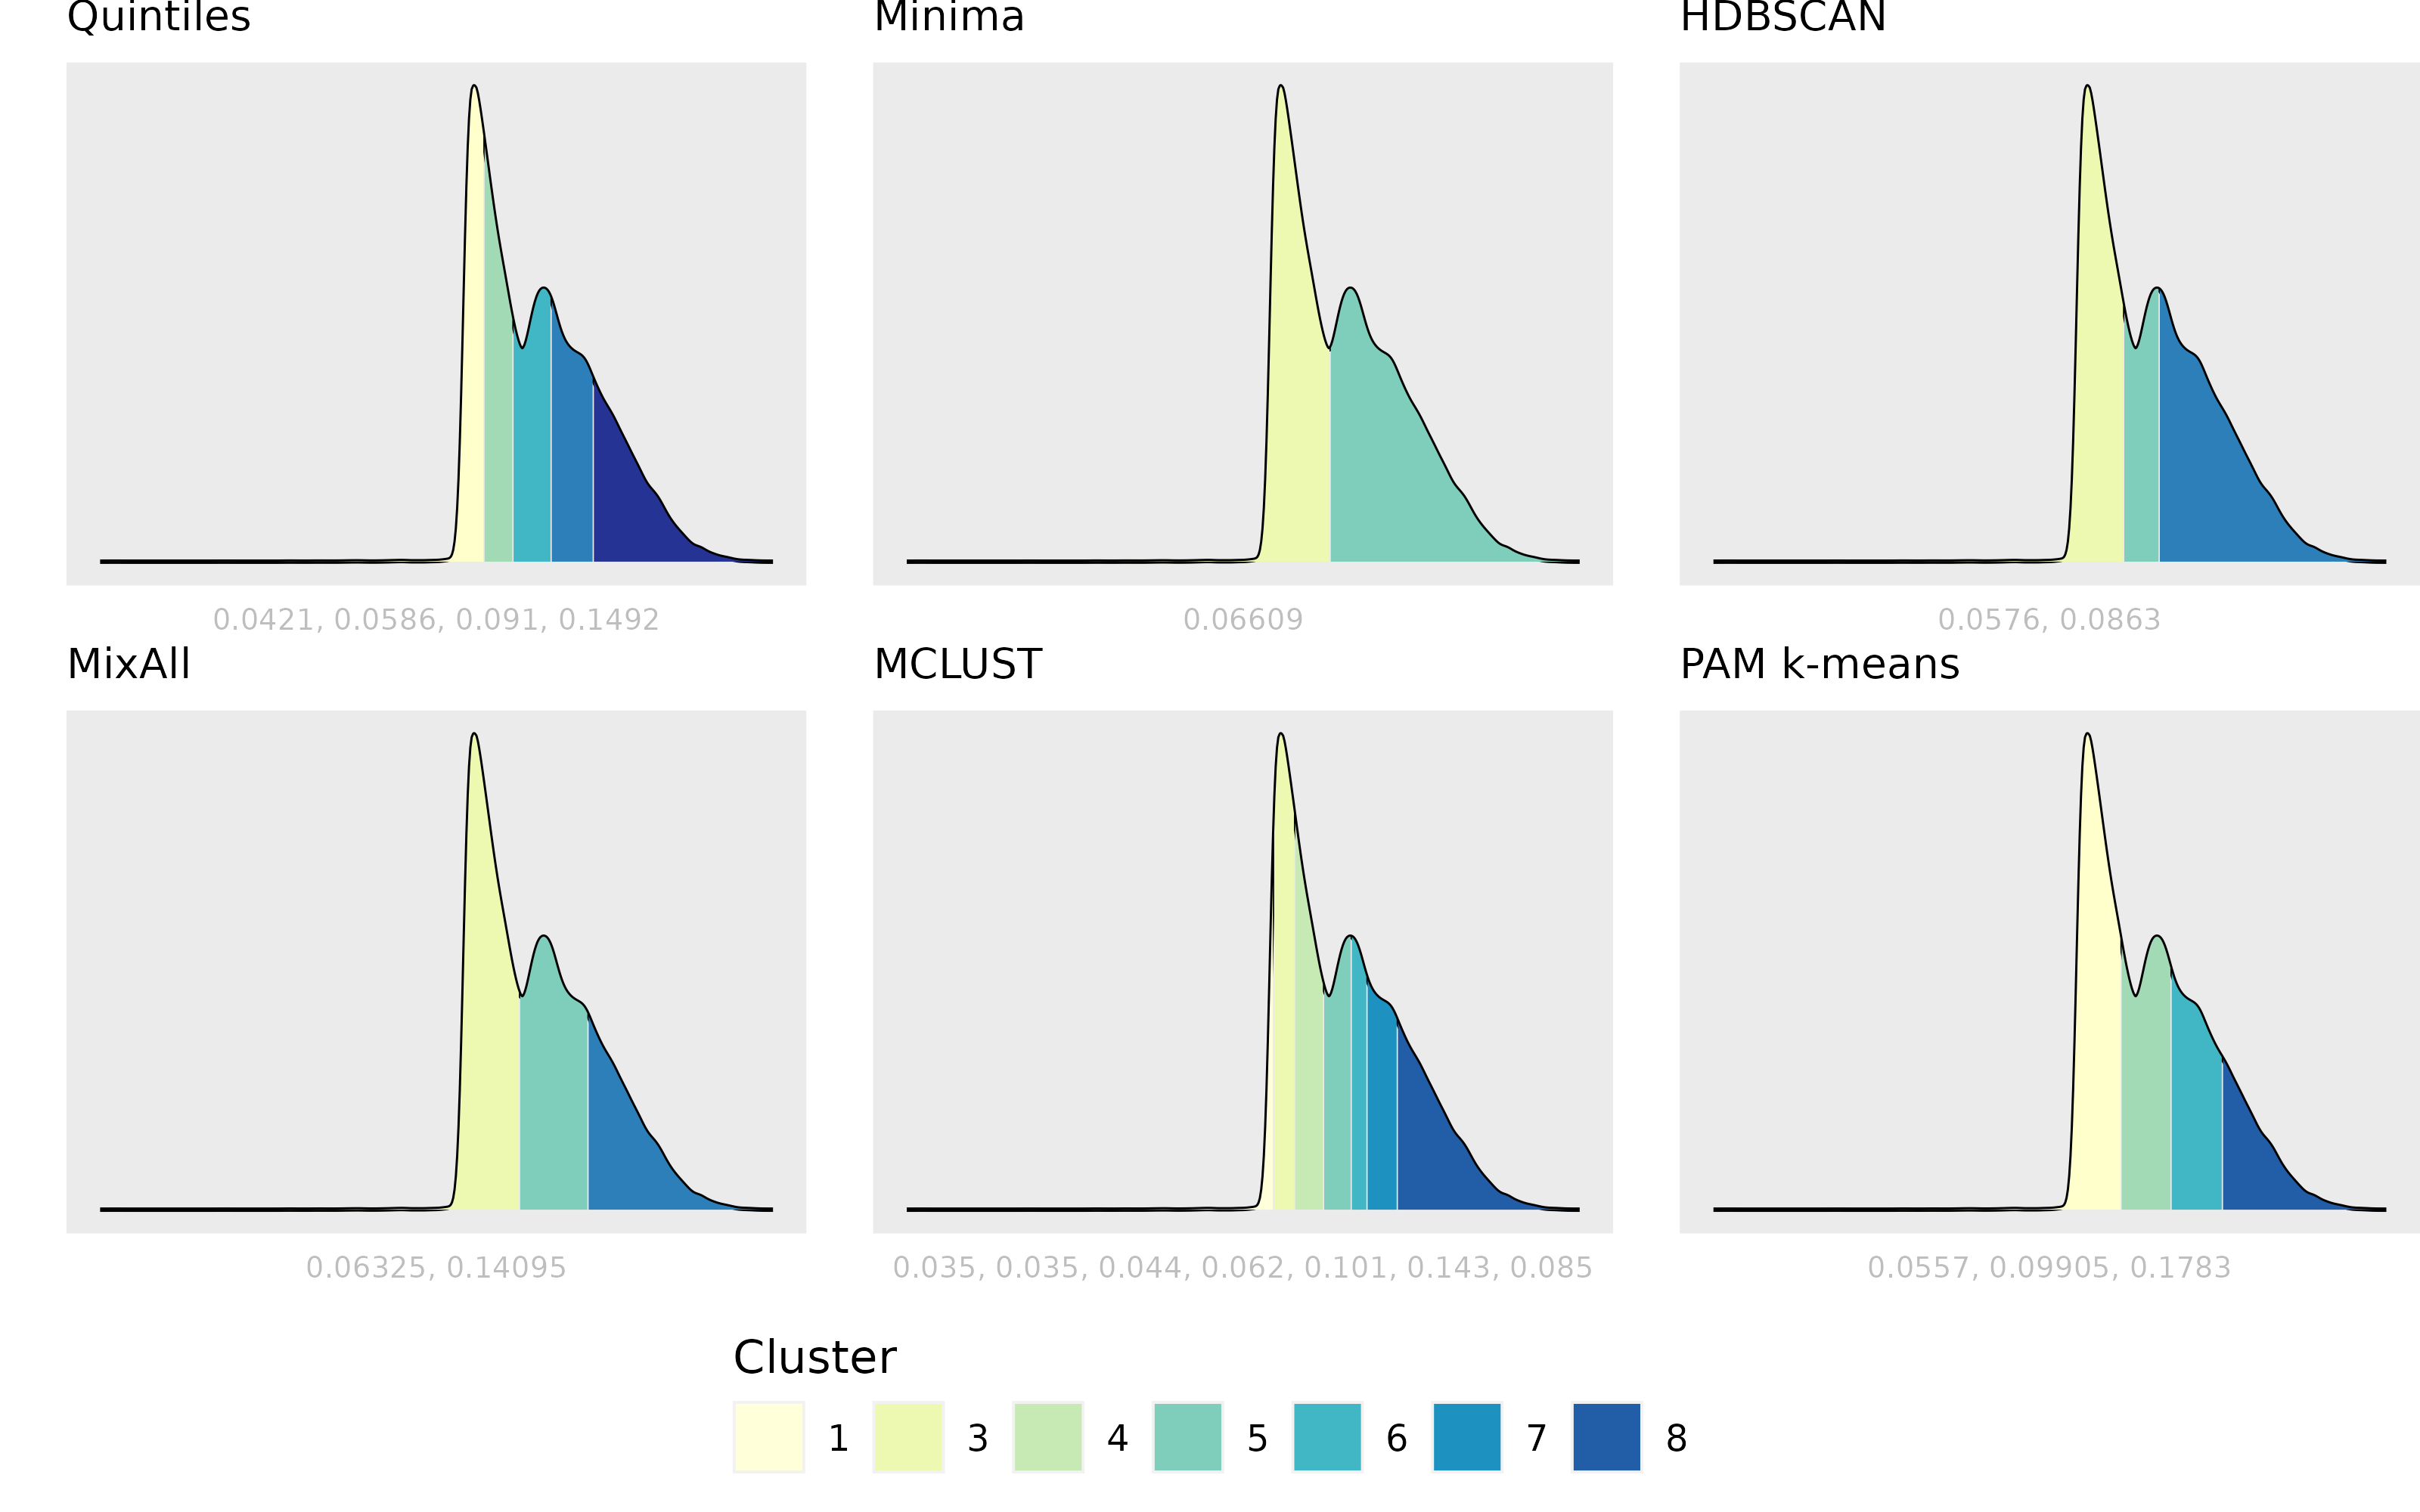
\includegraphics[width=\textwidth]{./cutoffs/by_amenity/Secondary Education_cutoffs.png}
\caption[Secondary education cutoffs]{Cut-offs values shown on the log-transformed density plots for all clustering approaches secondary education amenity.}\label{seceduccutoffs}
\end{figure}










\begin{figure}[H]
\centering
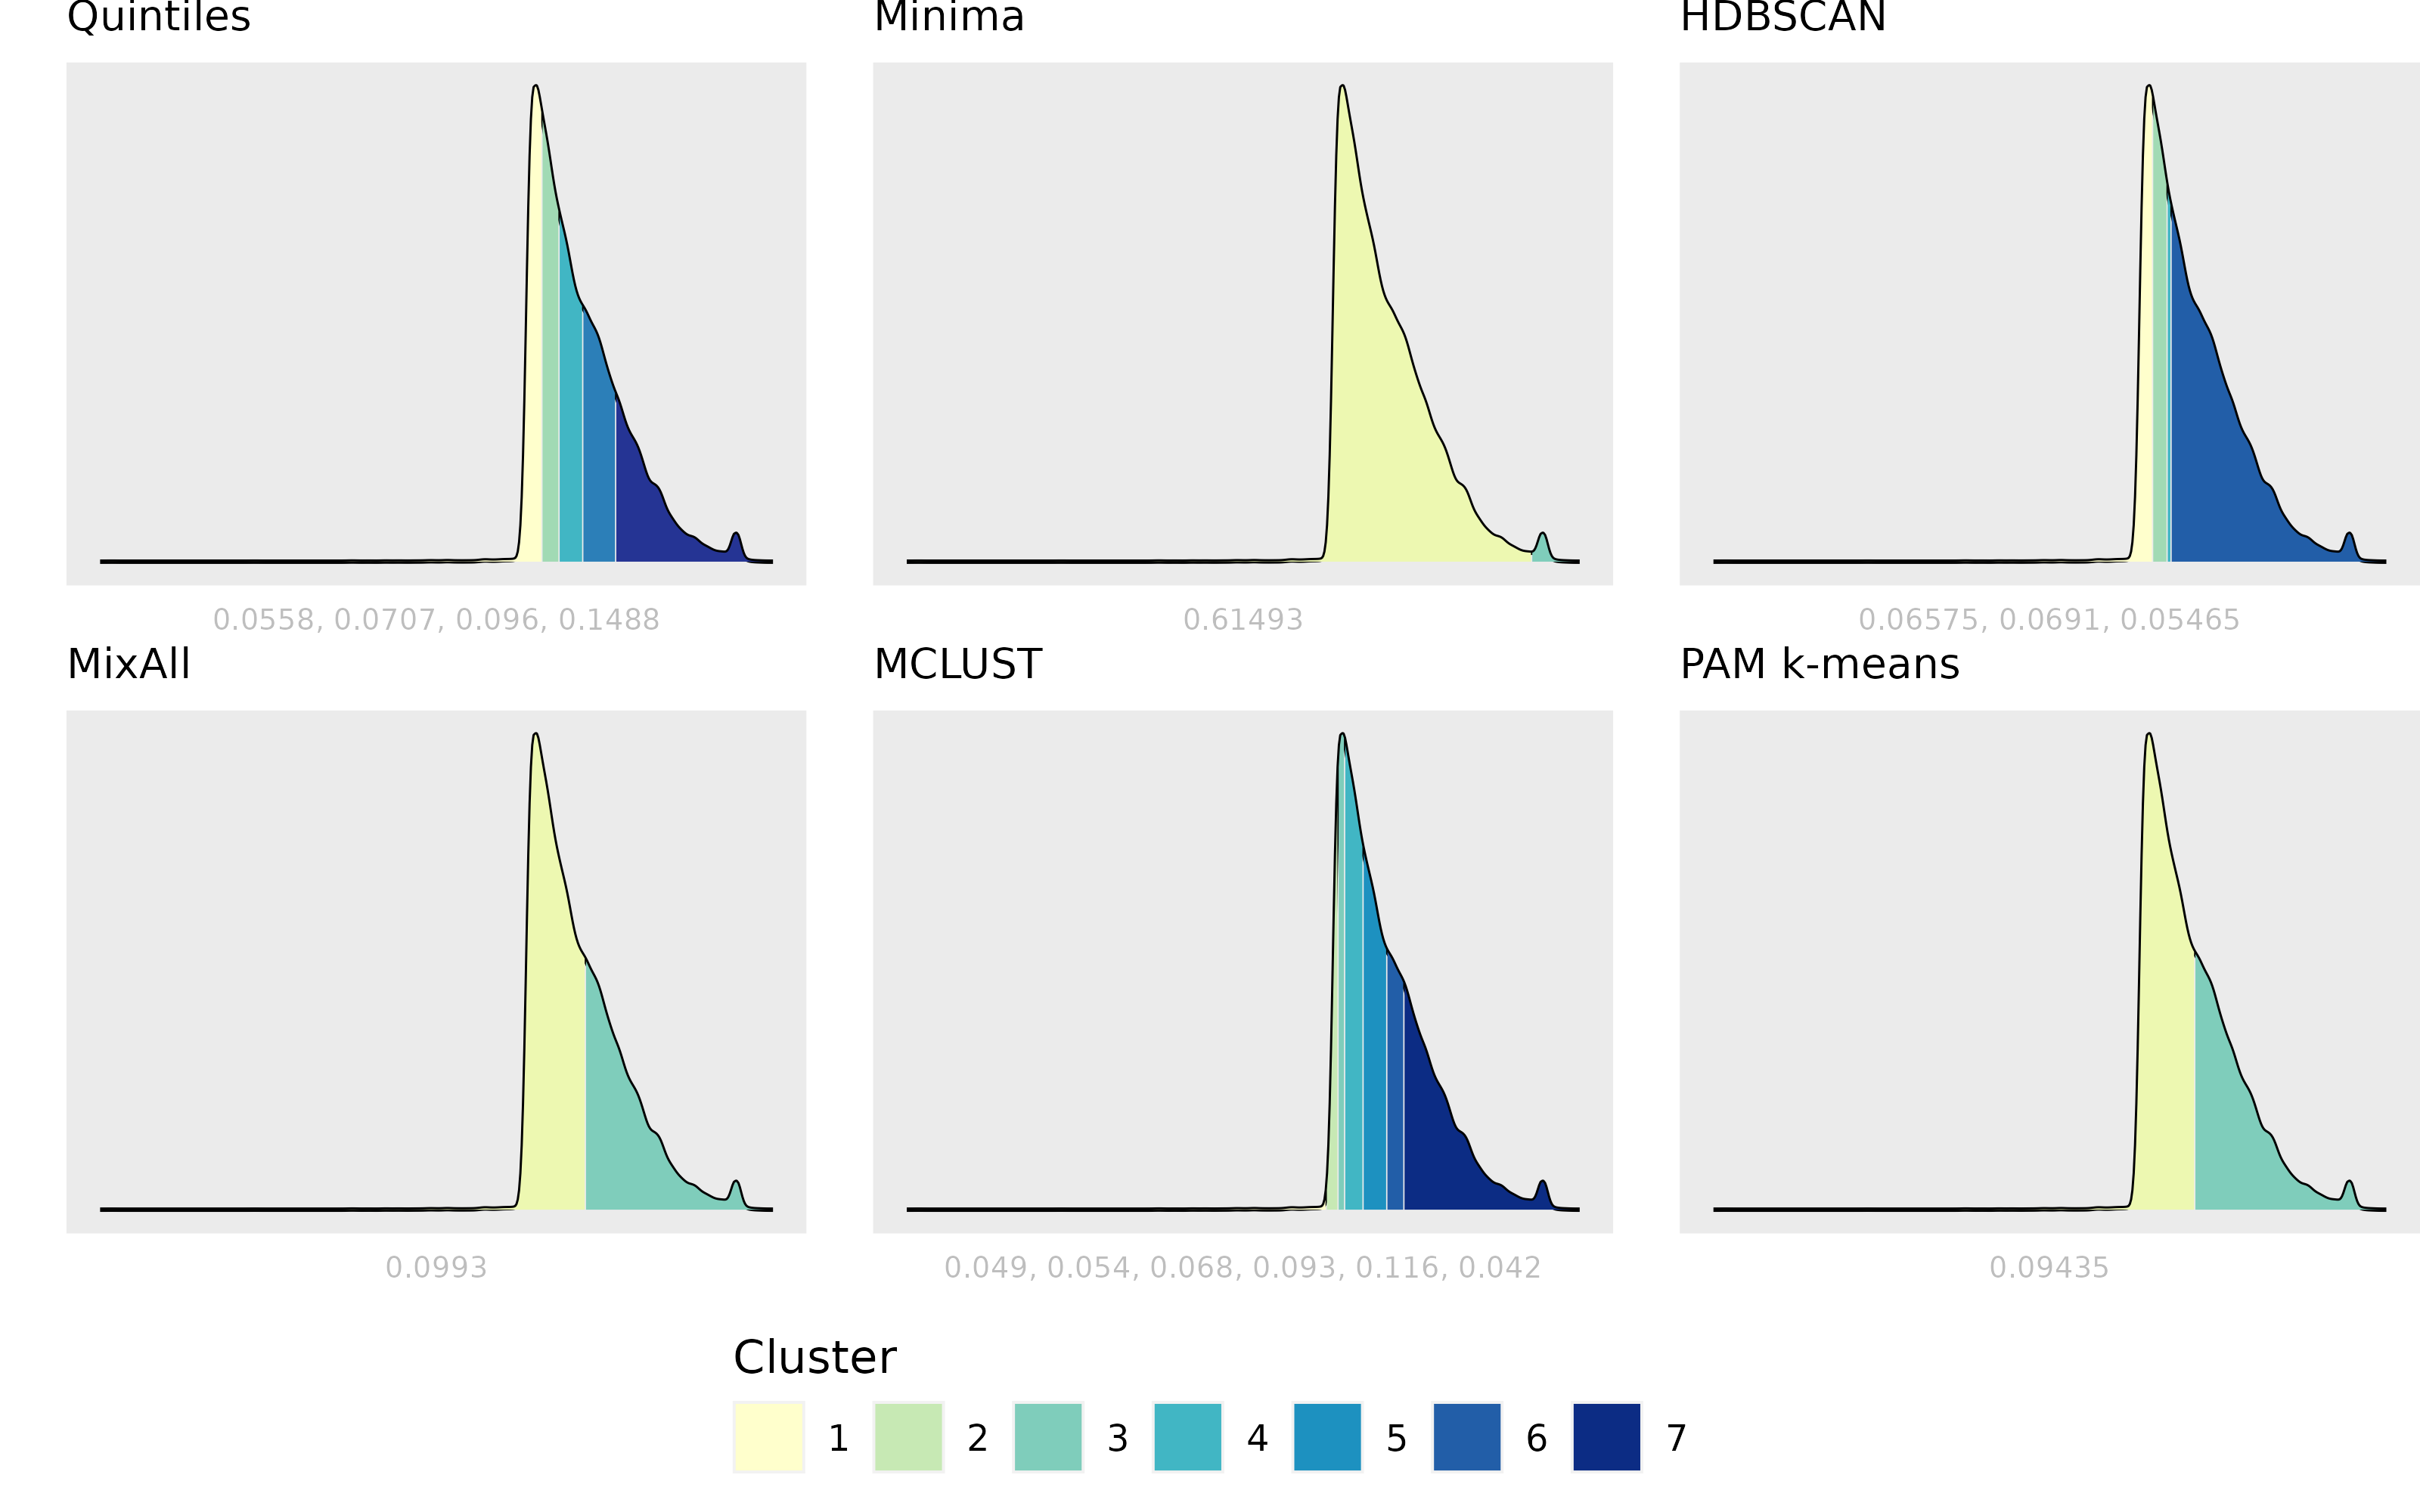
\includegraphics[width=\textwidth]{./cutoffs/by_amenity/Library_cutoffs.png}
\caption[Library cutoffs]{Cut-offs values shown on the log-transformed density plots for all clustering approaches library amenity.}\label{librarycutoffs}
\end{figure}










\begin{figure}[H]
\centering
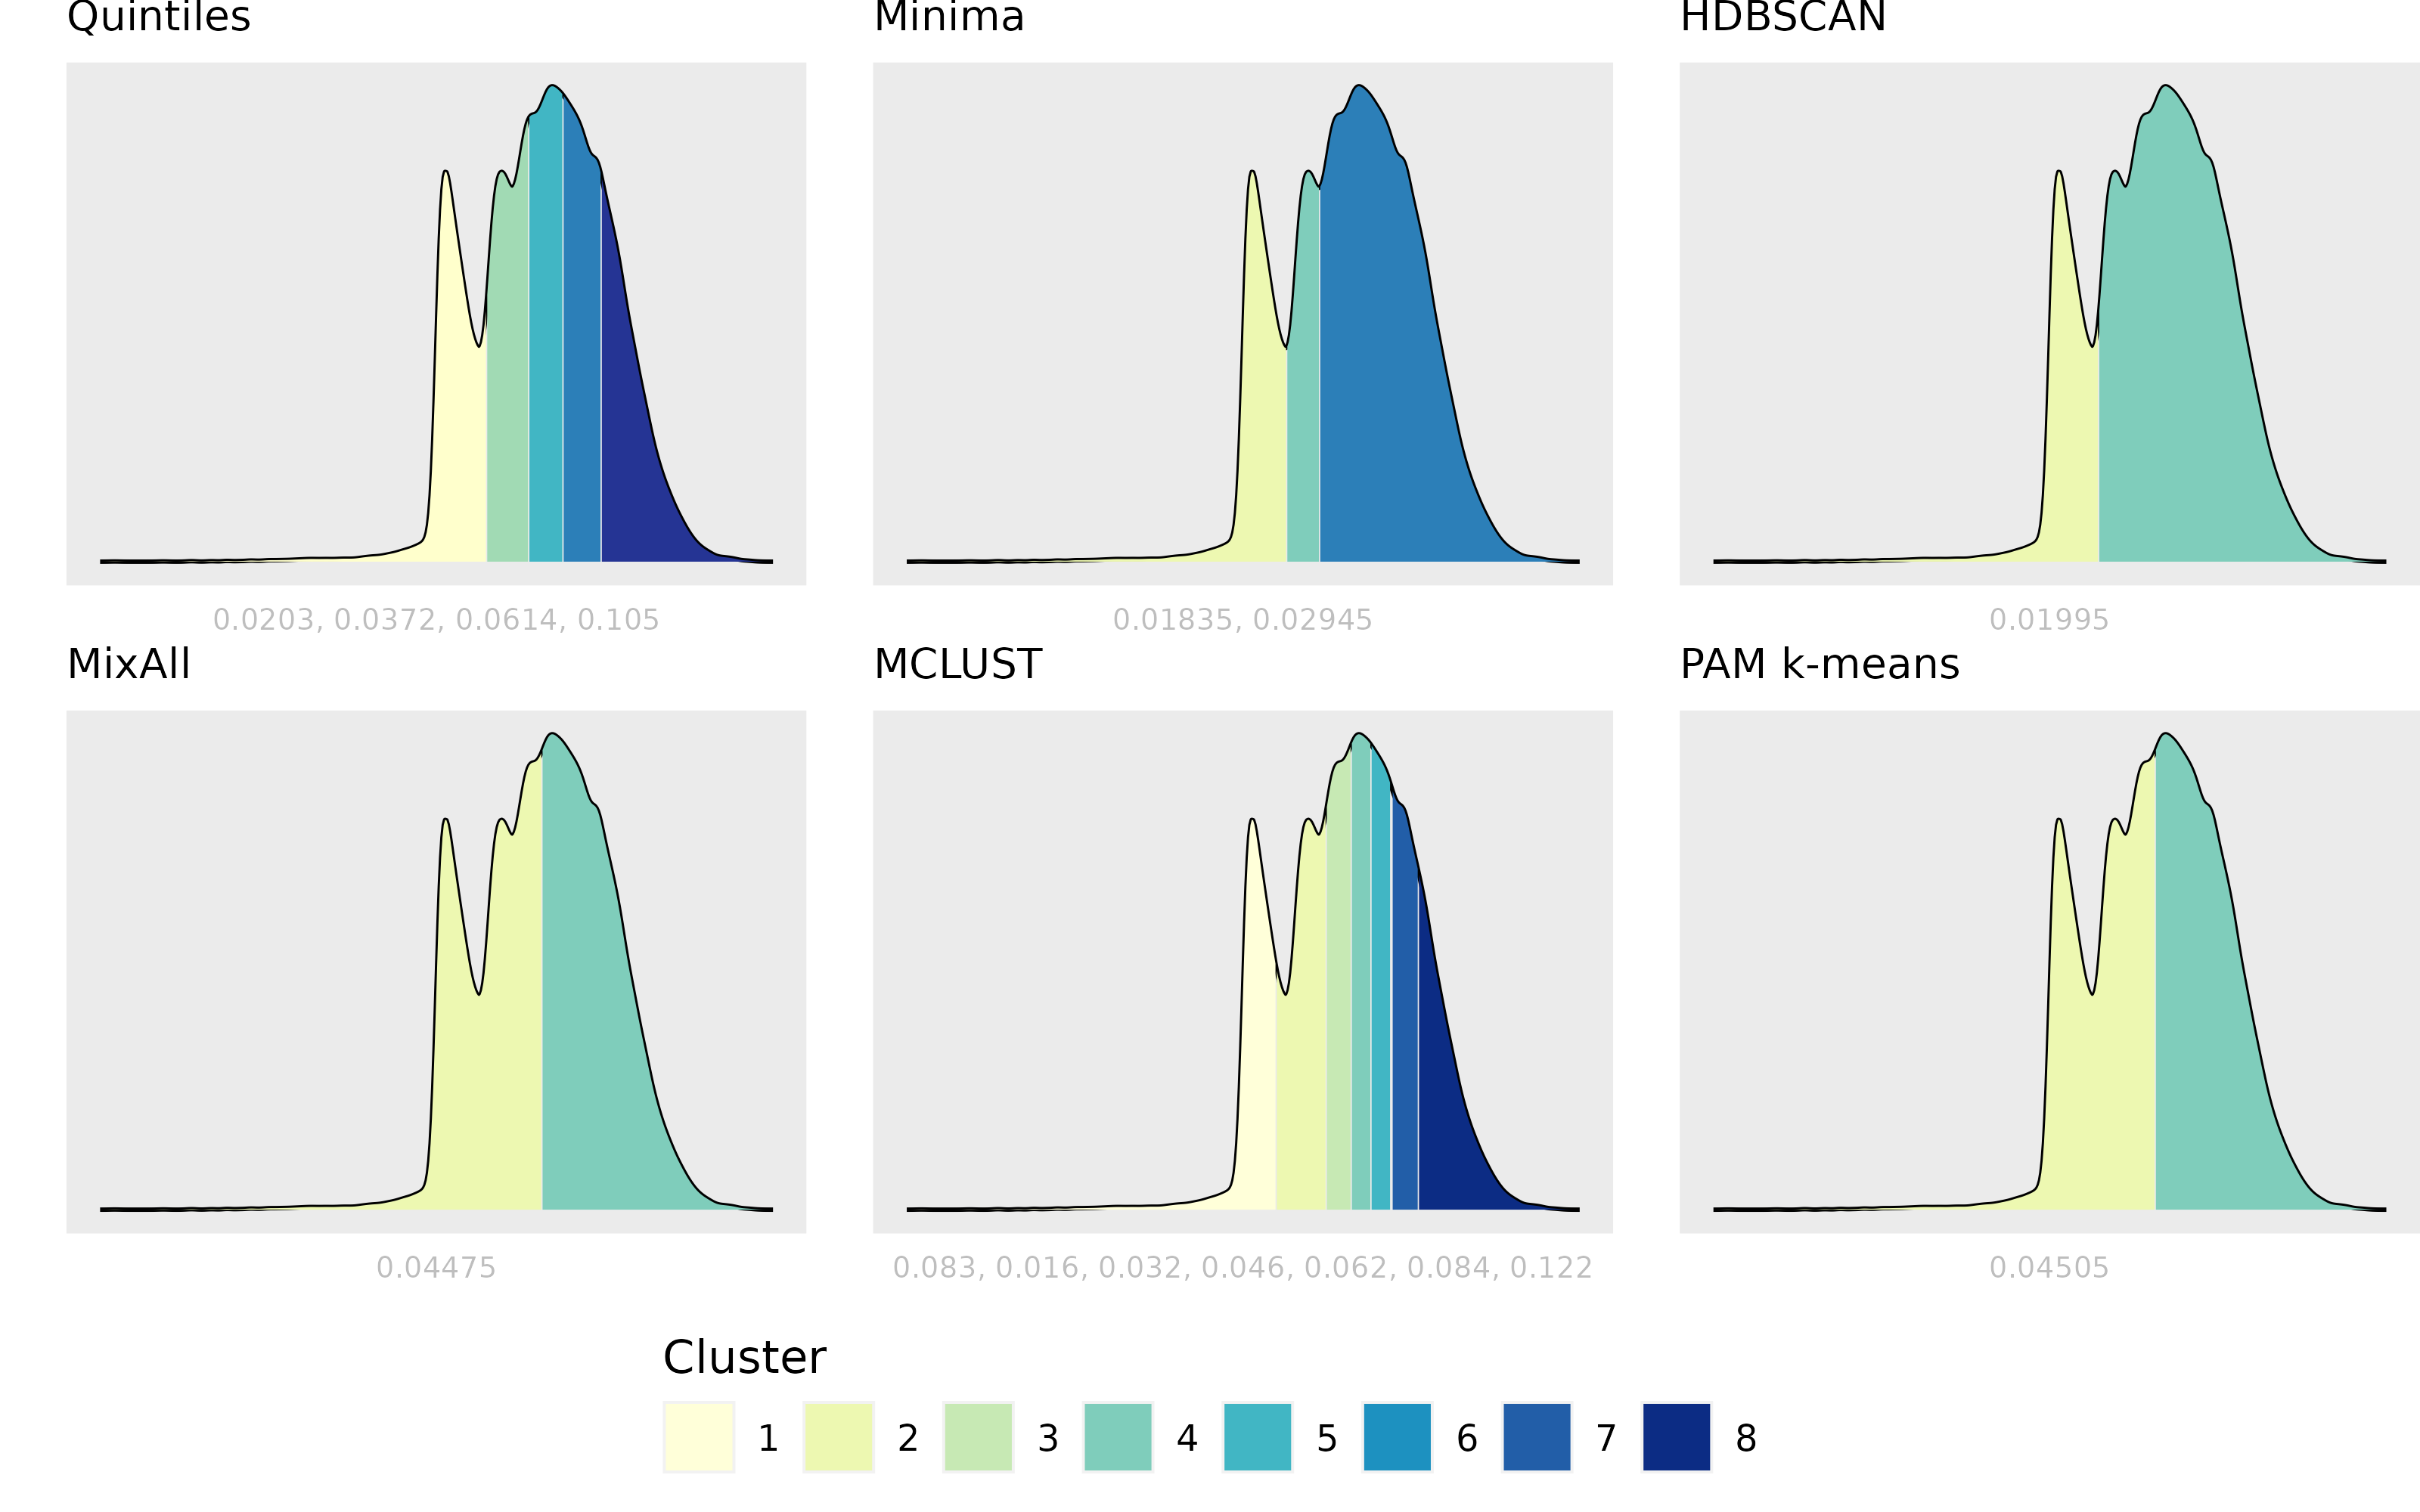
\includegraphics[width=\textwidth]{./cutoffs/by_amenity/Parks_cutoffs.png}
\caption[Parks cutoffs]{Cut-offs values shown on the log-transformed density plots for all clustering approaches parks amenity.}\label{parkscutoffs}
\end{figure}










\begin{figure}[H]
\centering
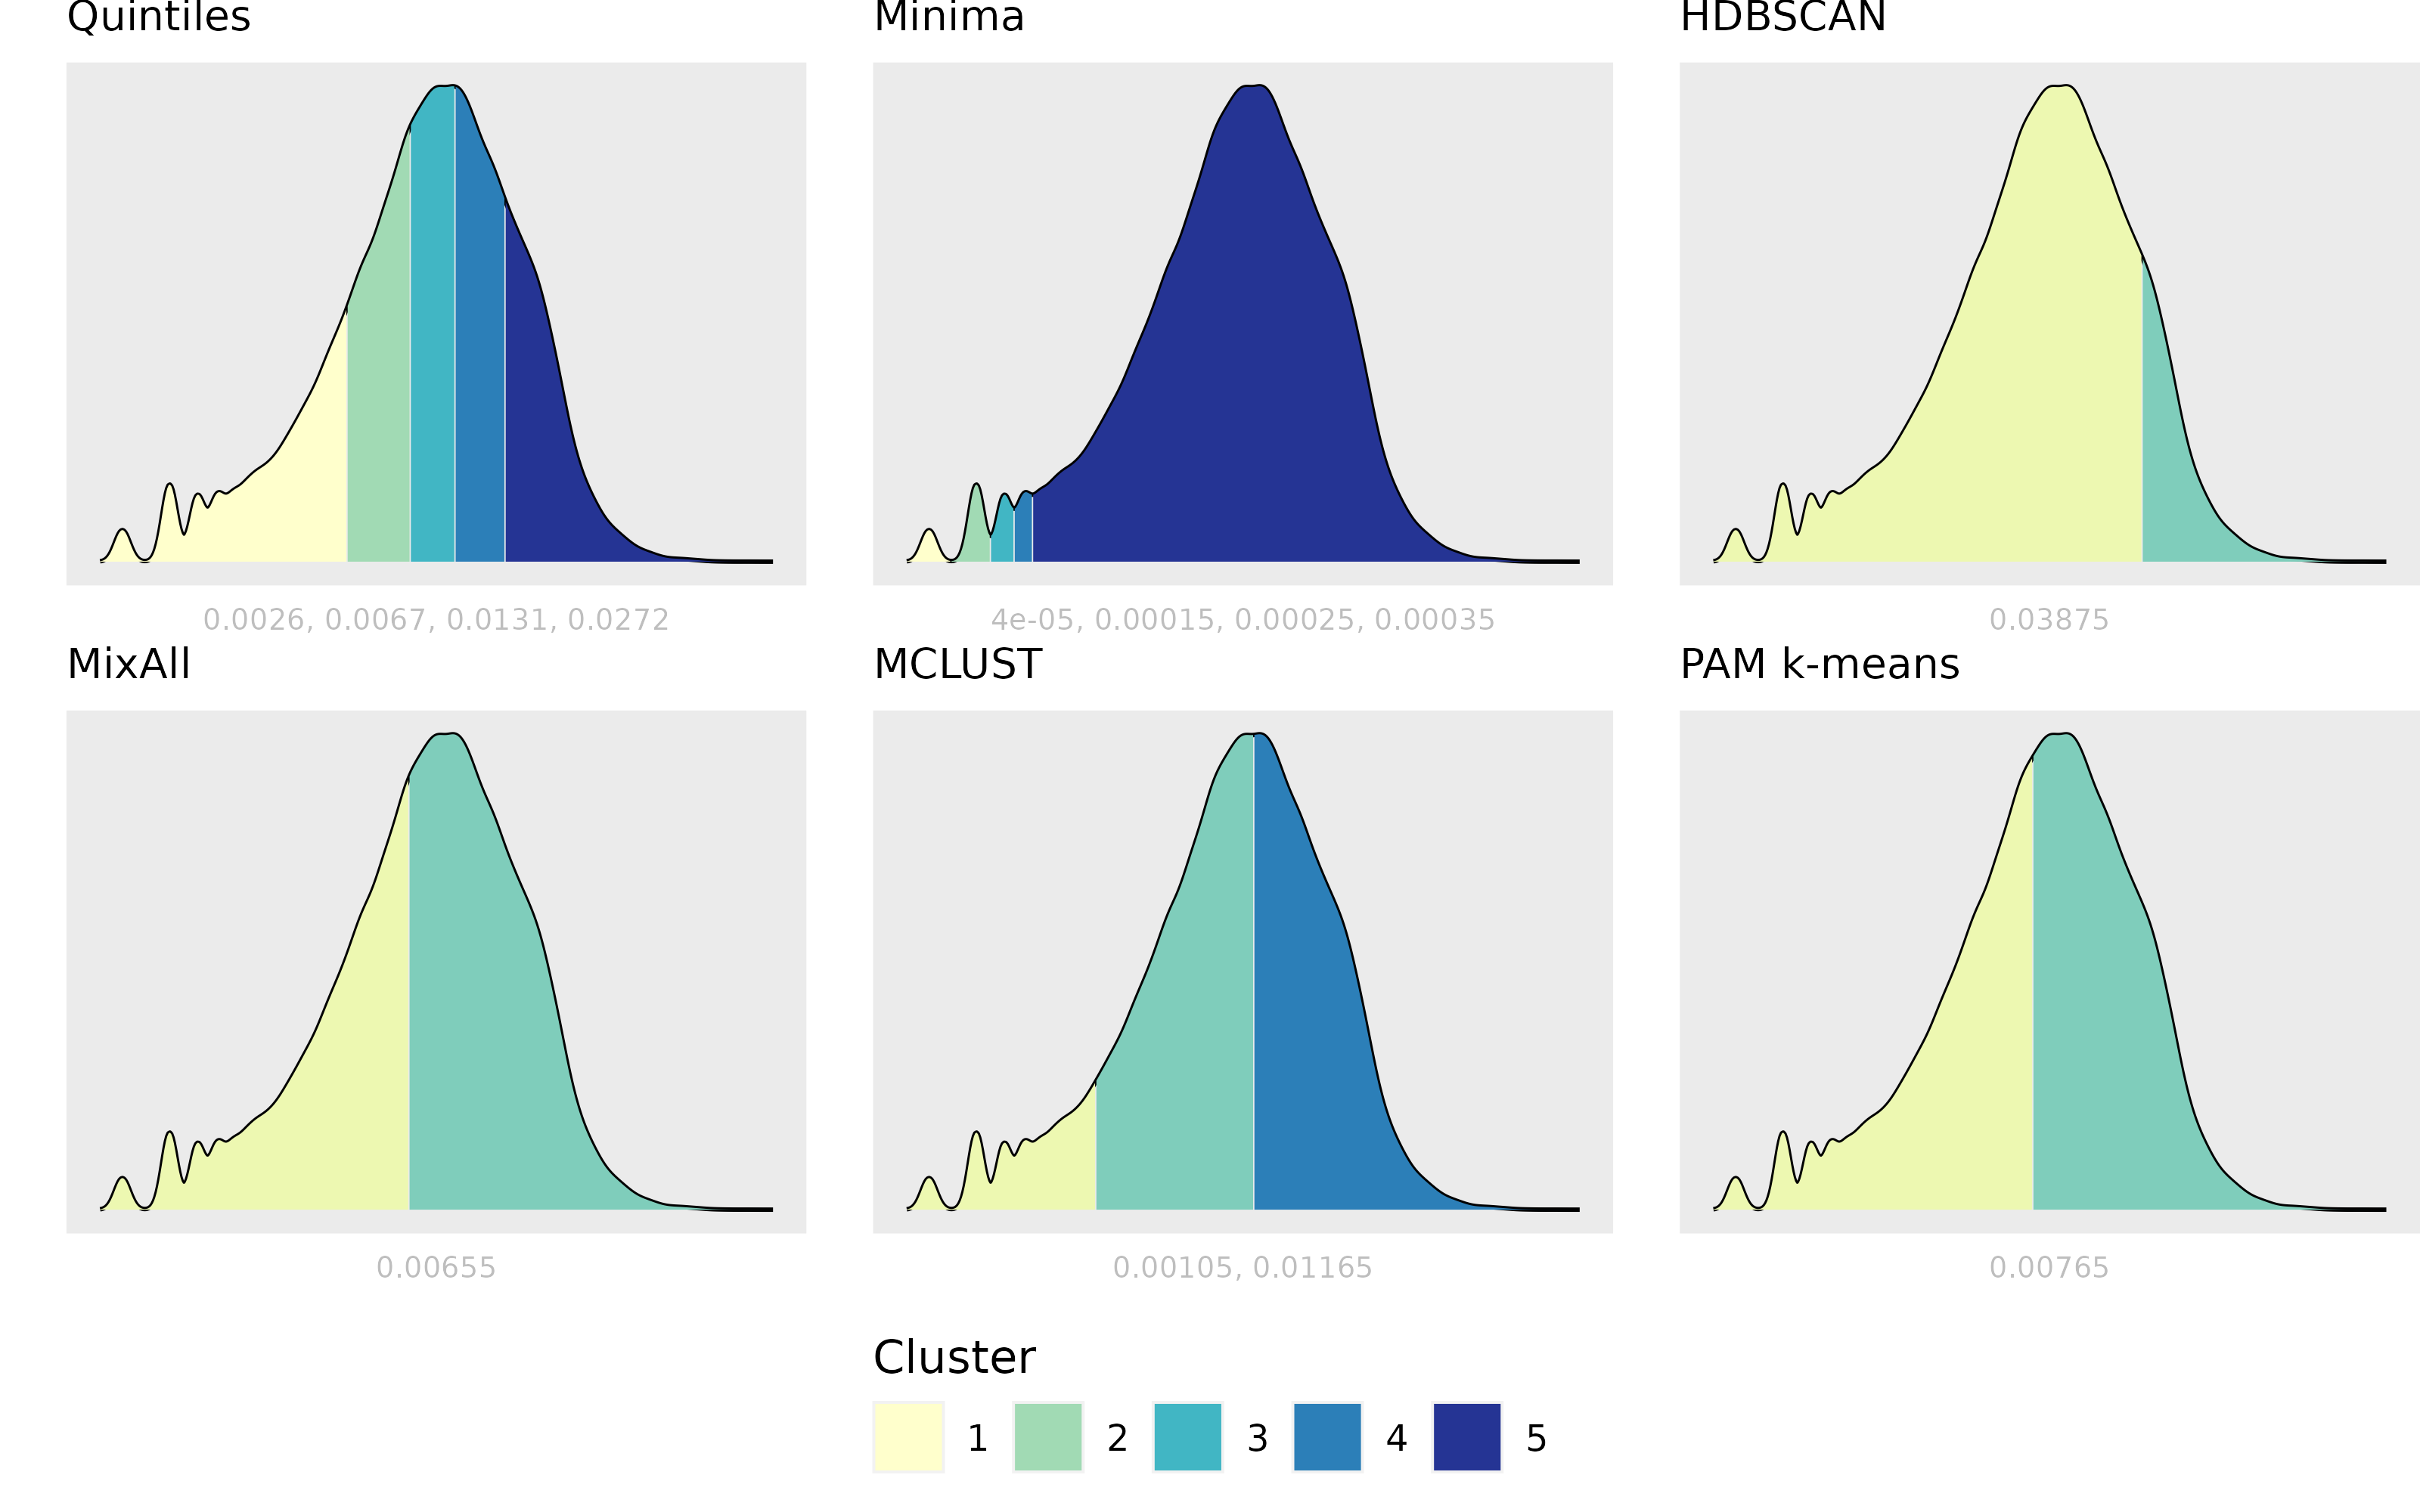
\includegraphics[width=\textwidth]{./cutoffs/by_amenity/Transit_cutoffs.png}
\caption[Transit cutoffs]{Cut-offs values shown on the log-transformed density plots for all clustering approaches transit amenity.}\label{transitcutoffs}
\end{figure}













\begin{figure}[H]
\centering
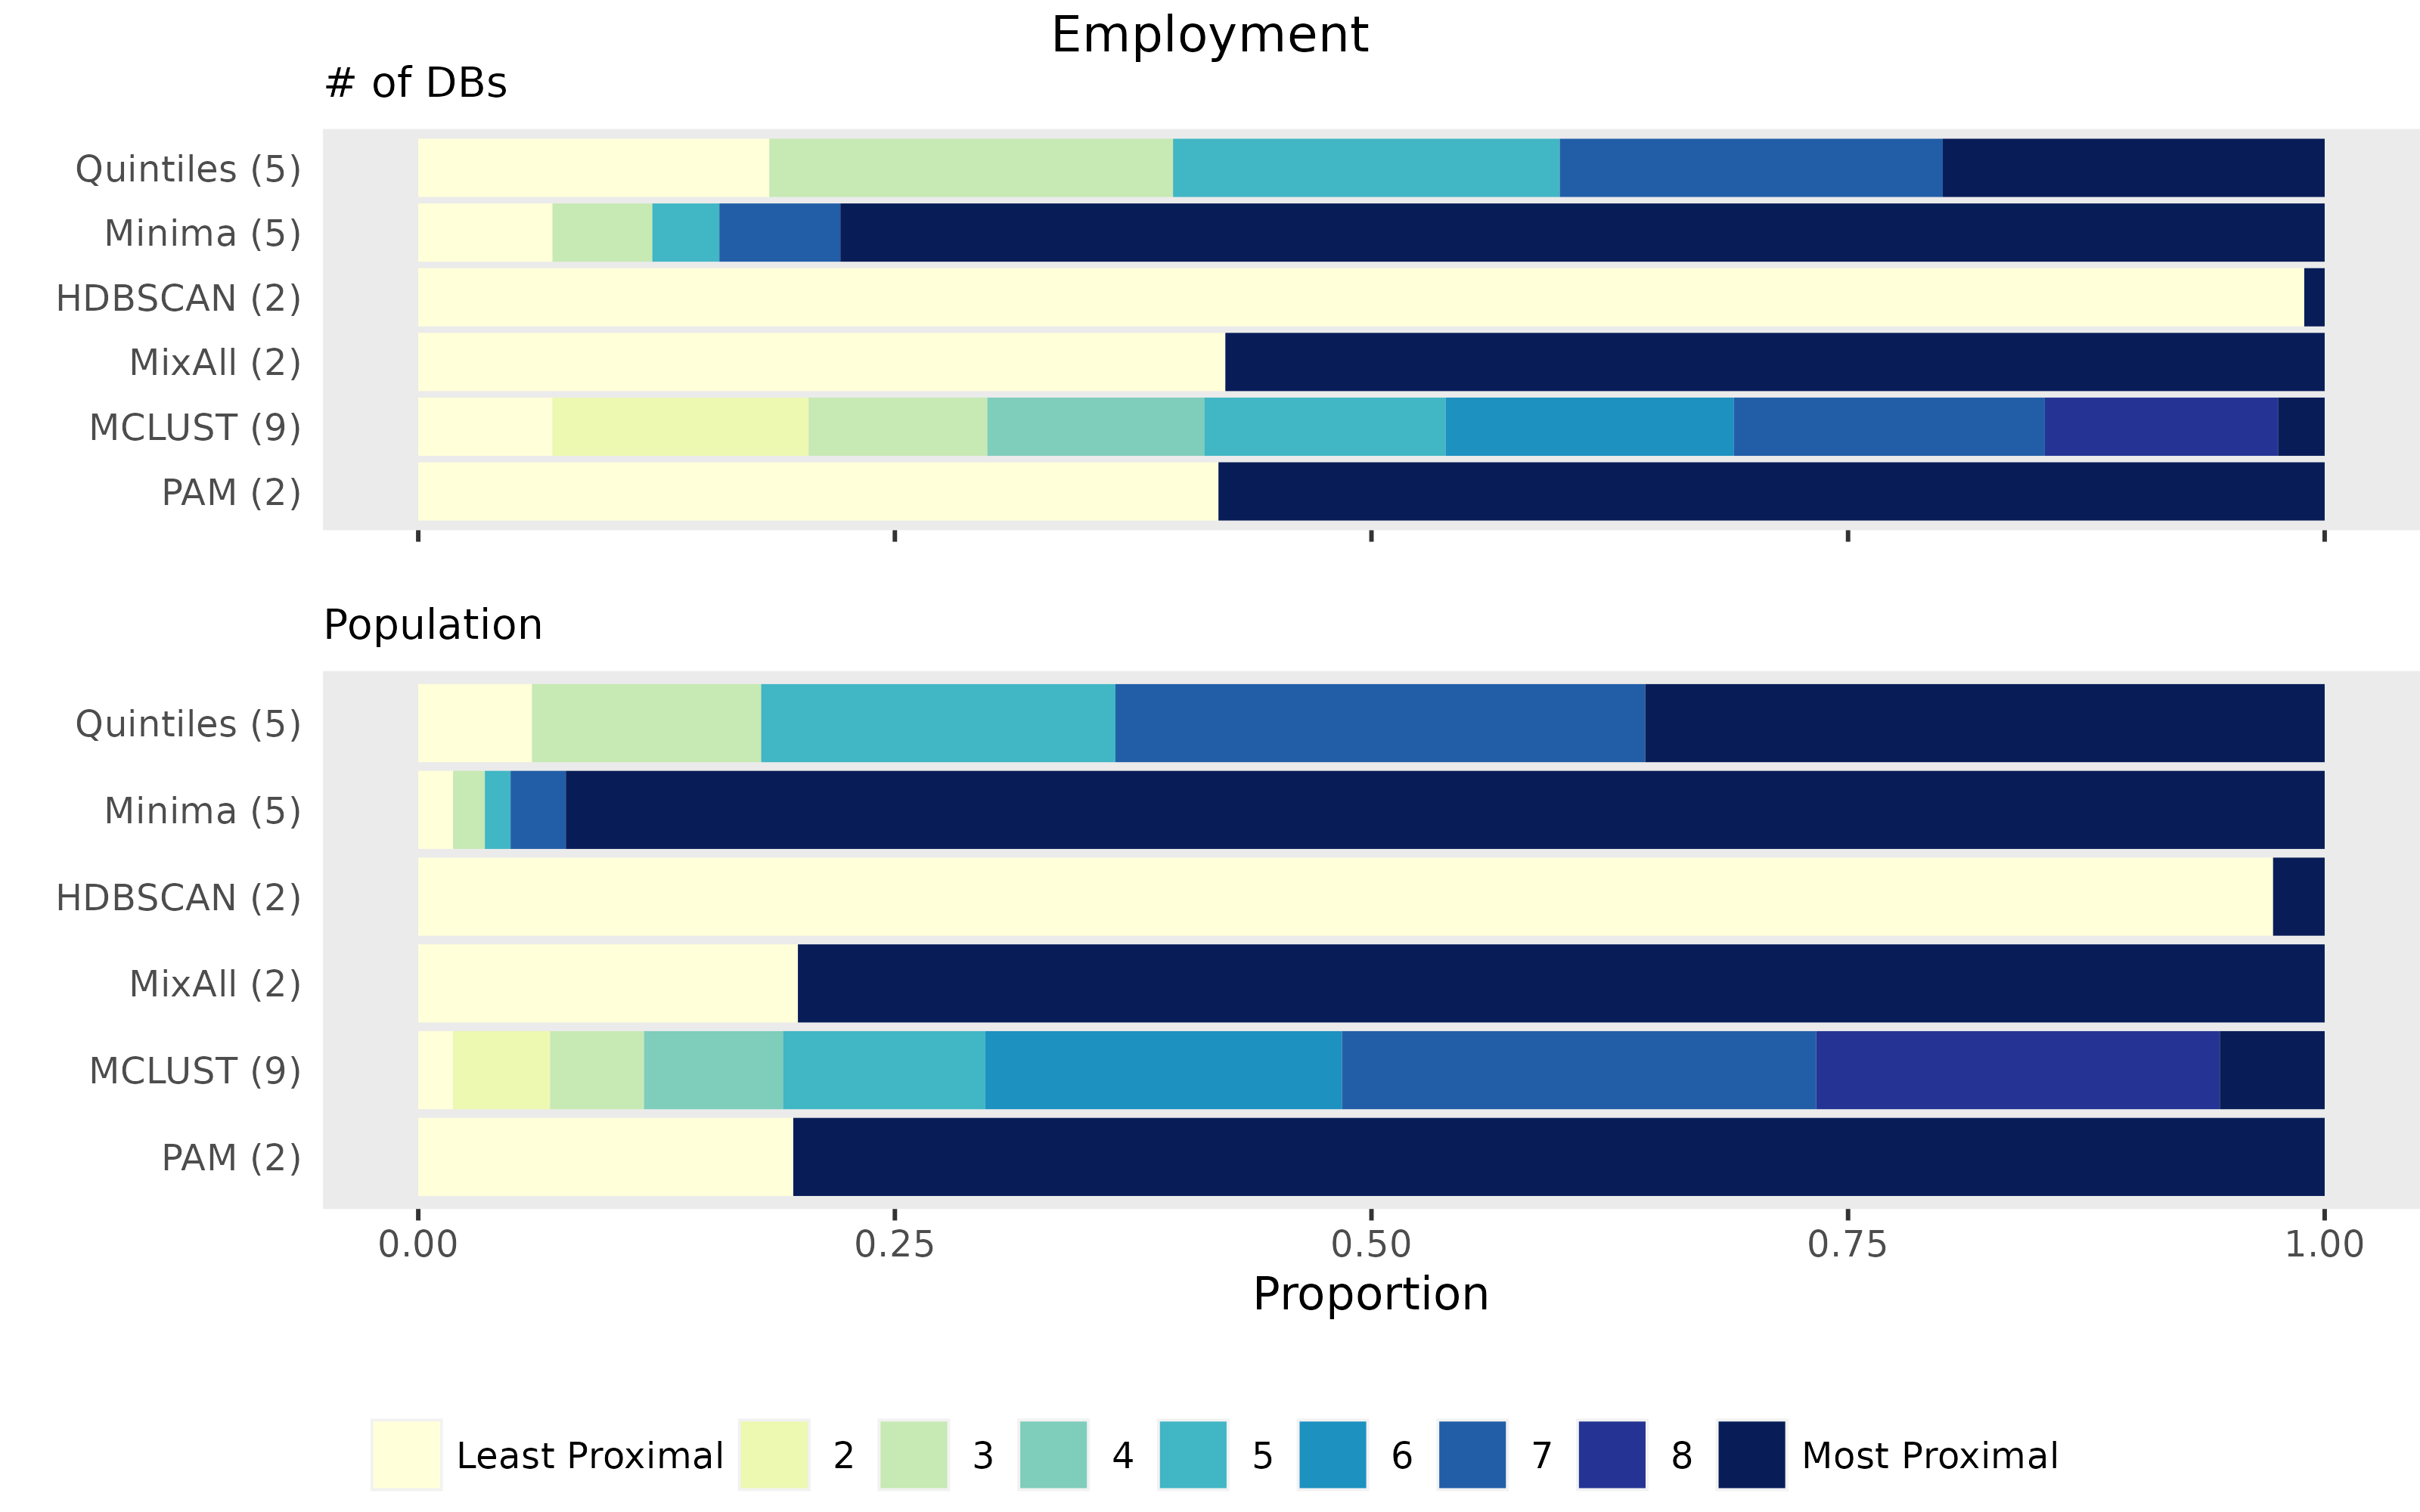
\includegraphics[width=\textwidth]{./barplot_comparison/Employment_barplot.png}
\caption[Employment profile barplot]{Proportion of DBs and population in each cluster for all approaches for the employment amenity.}\label{employmentbarplot}
\end{figure}








\begin{figure}[H]
\centering
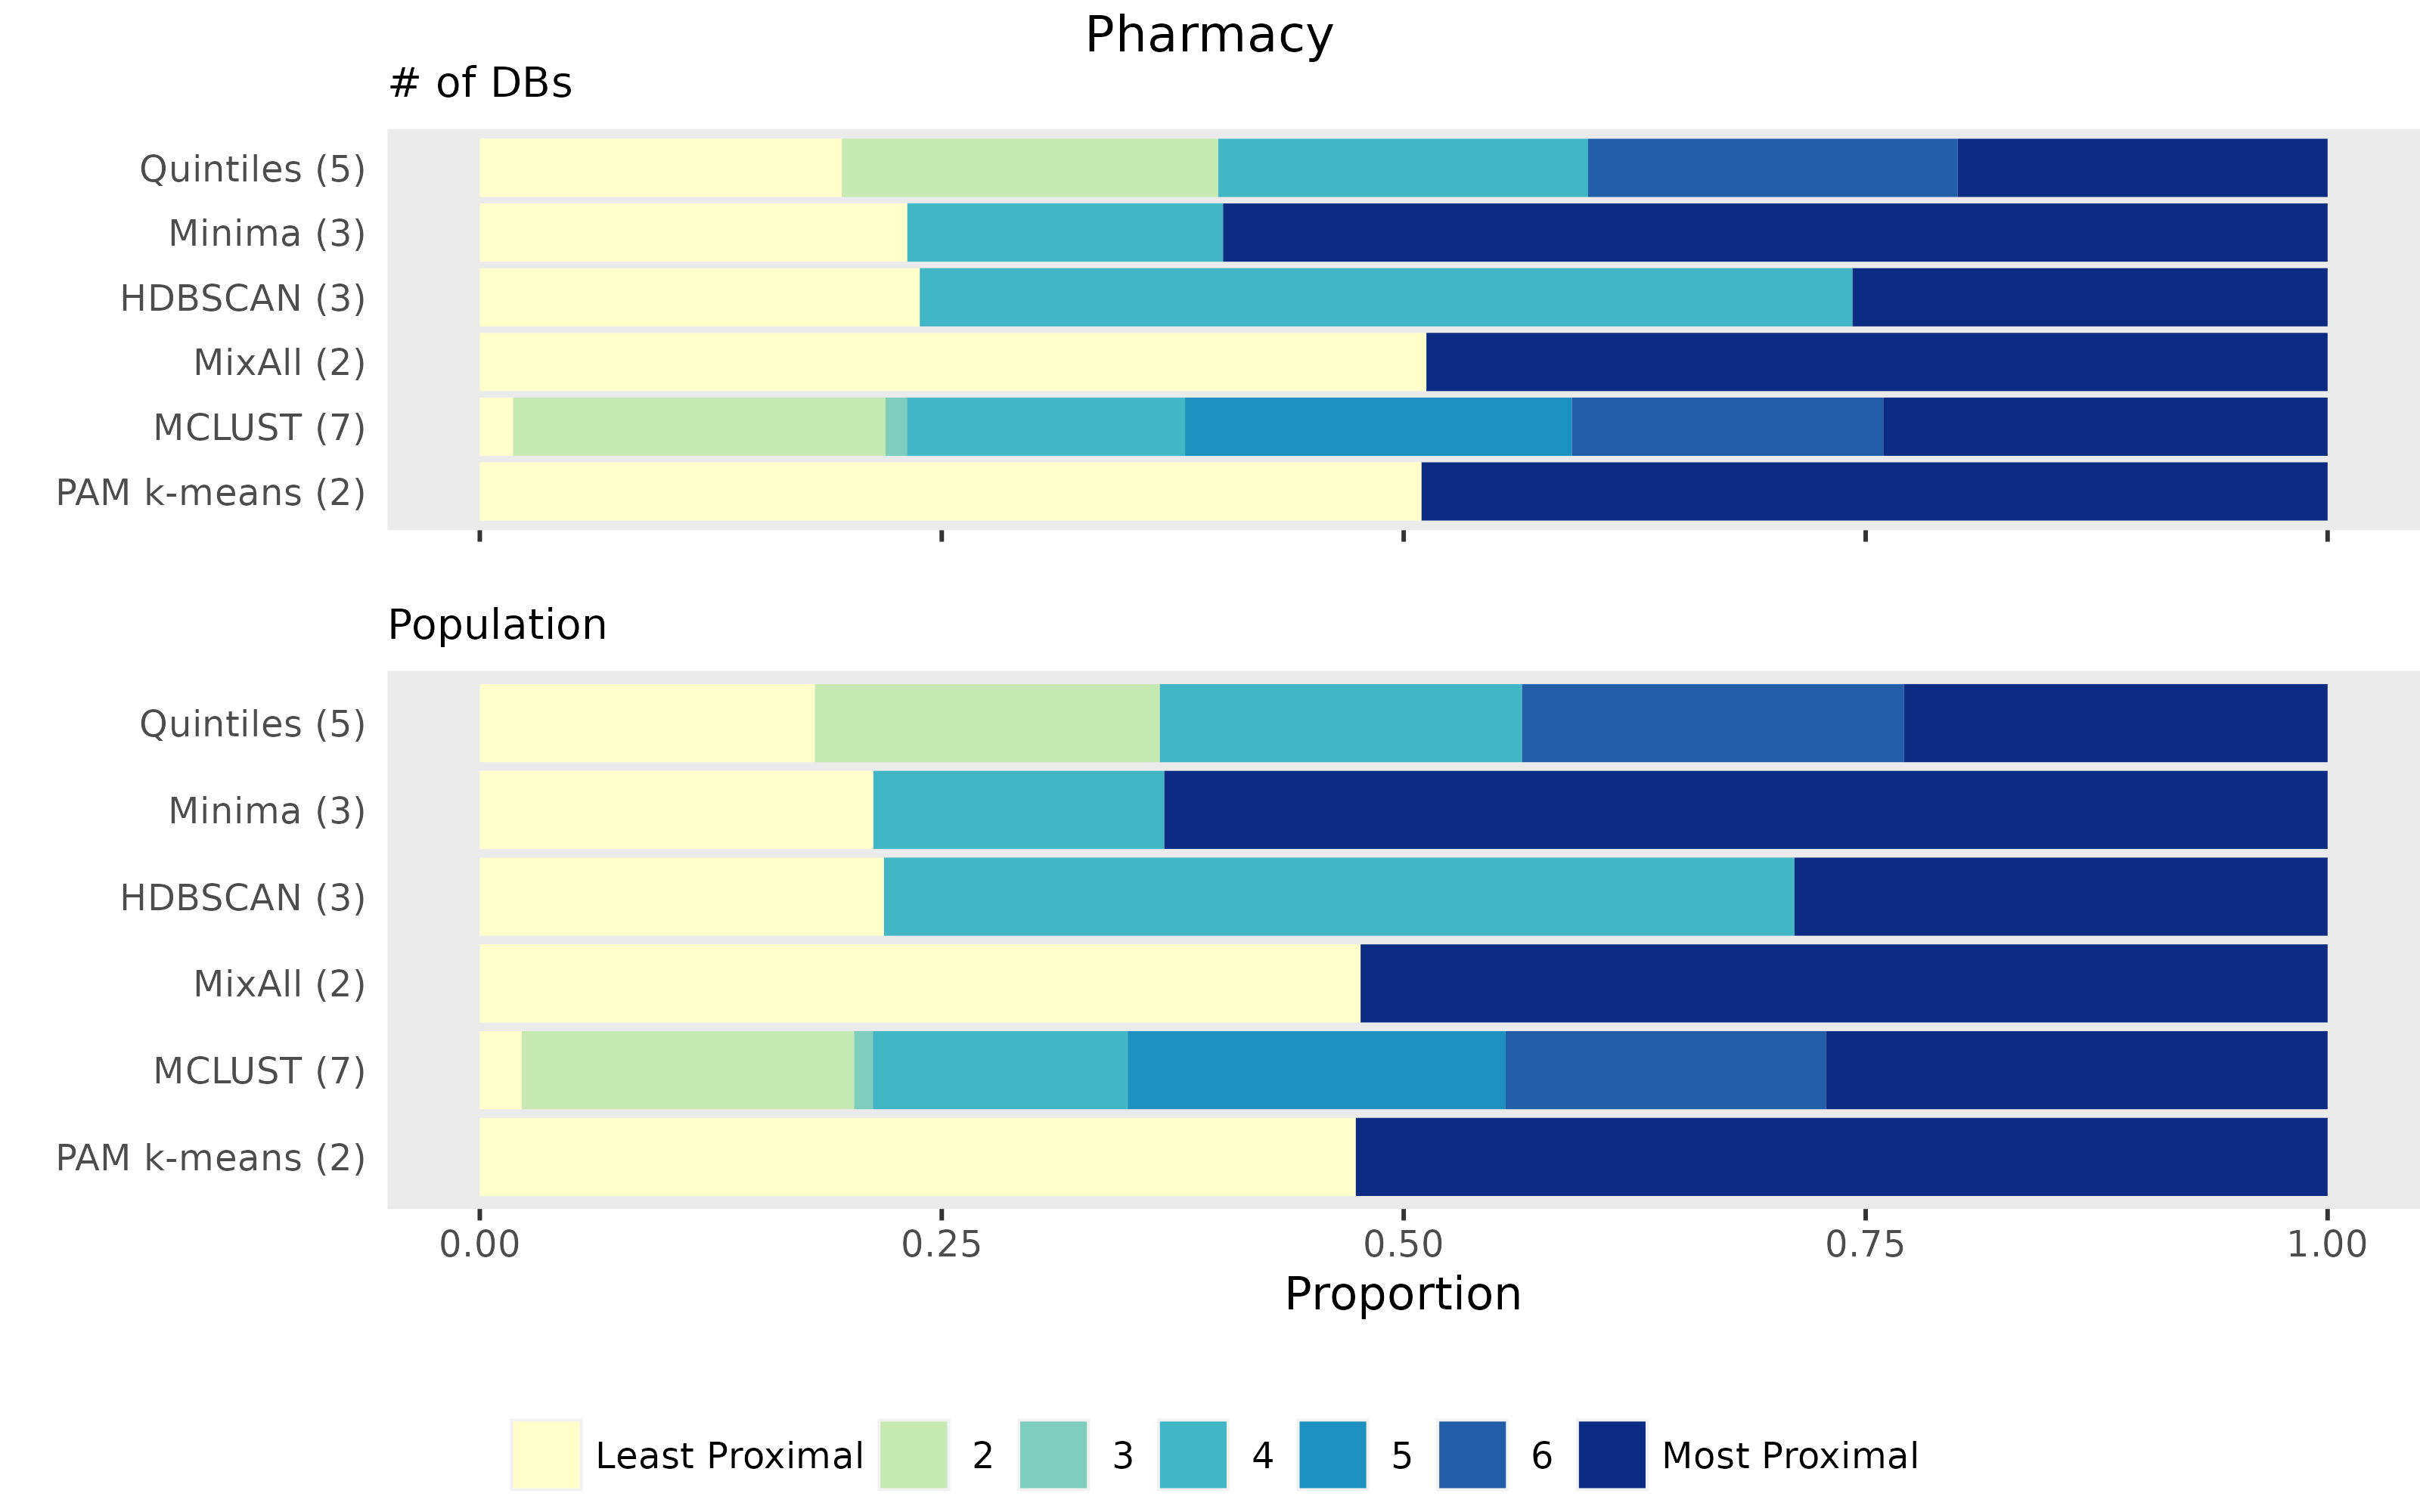
\includegraphics[width=\textwidth]{./barplot_comparison/Pharmacy_barplot.png}
\caption[Pharmacy profile barplot]{Proportion of DBs and population in each cluster for all approaches for the pharmacy amenity.}\label{pharmacybarplot}
\end{figure}









\begin{figure}[H]
\centering
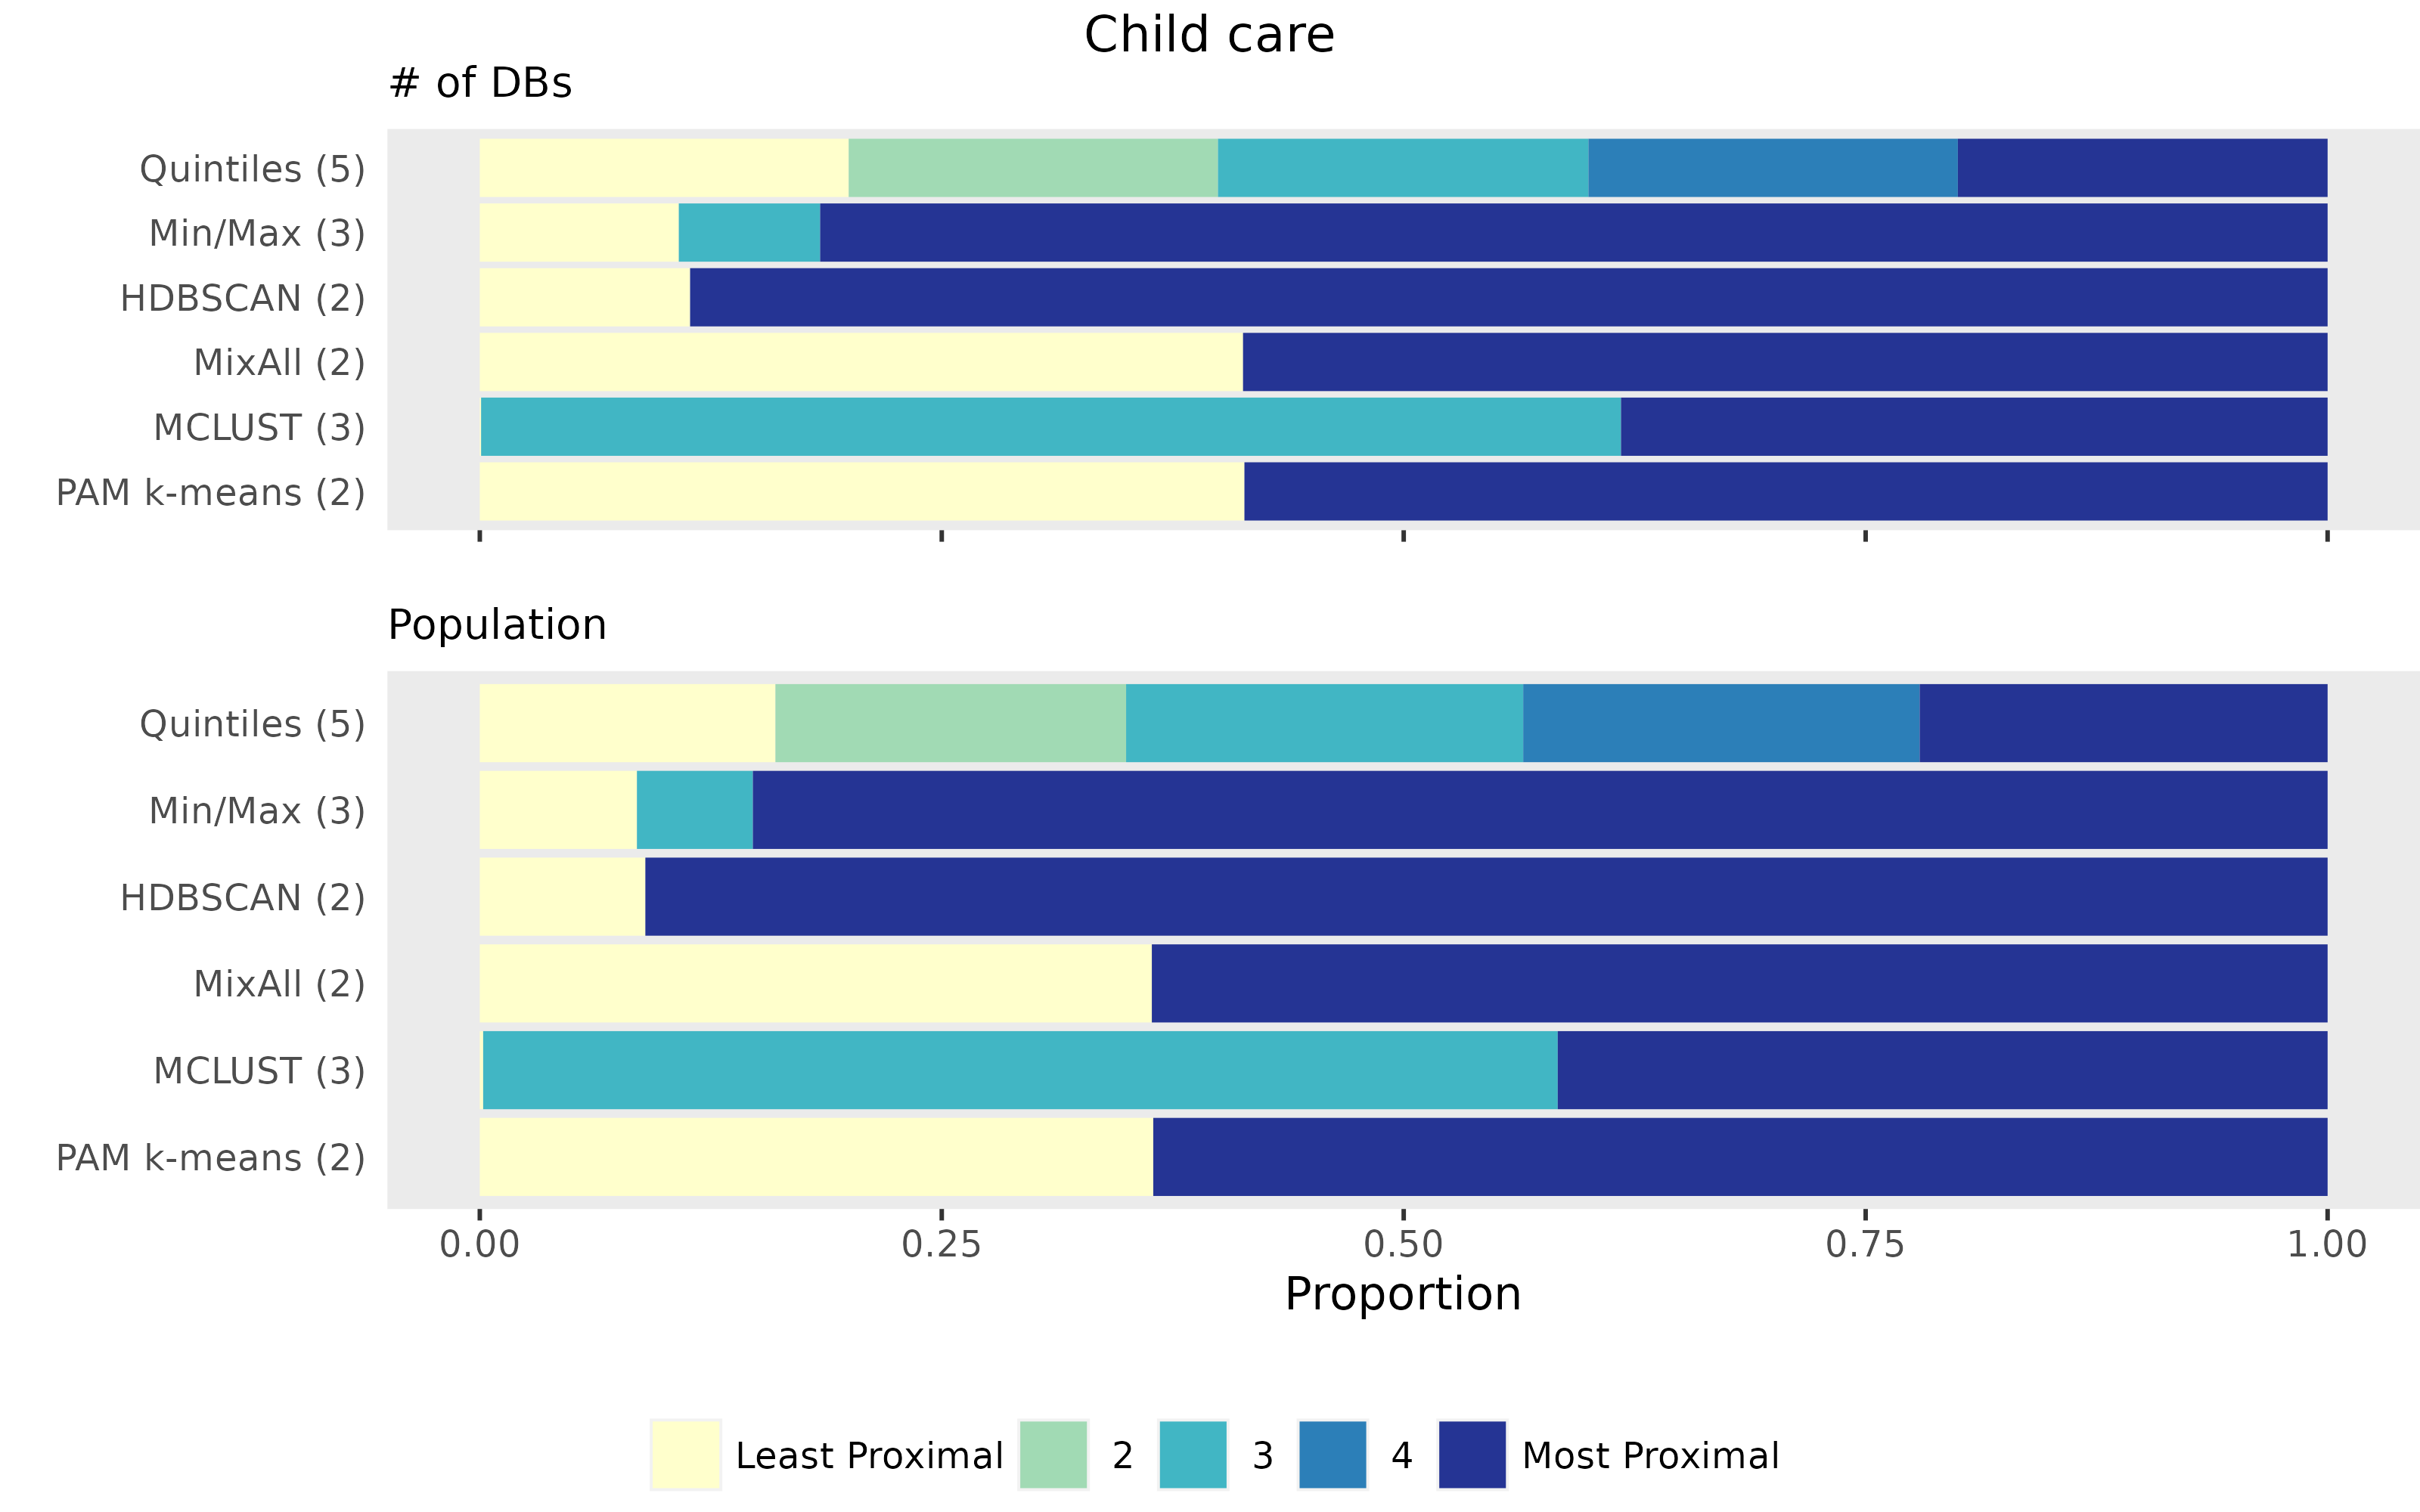
\includegraphics[width=\textwidth]{./barplot_comparison/Child care_barplot.png}
\caption[Child care profile barplot]{Proportion of DBs and population in each cluster for all approaches for the child care amenity.}\label{childcarebarplot}
\end{figure}









\begin{figure}[H]
\centering
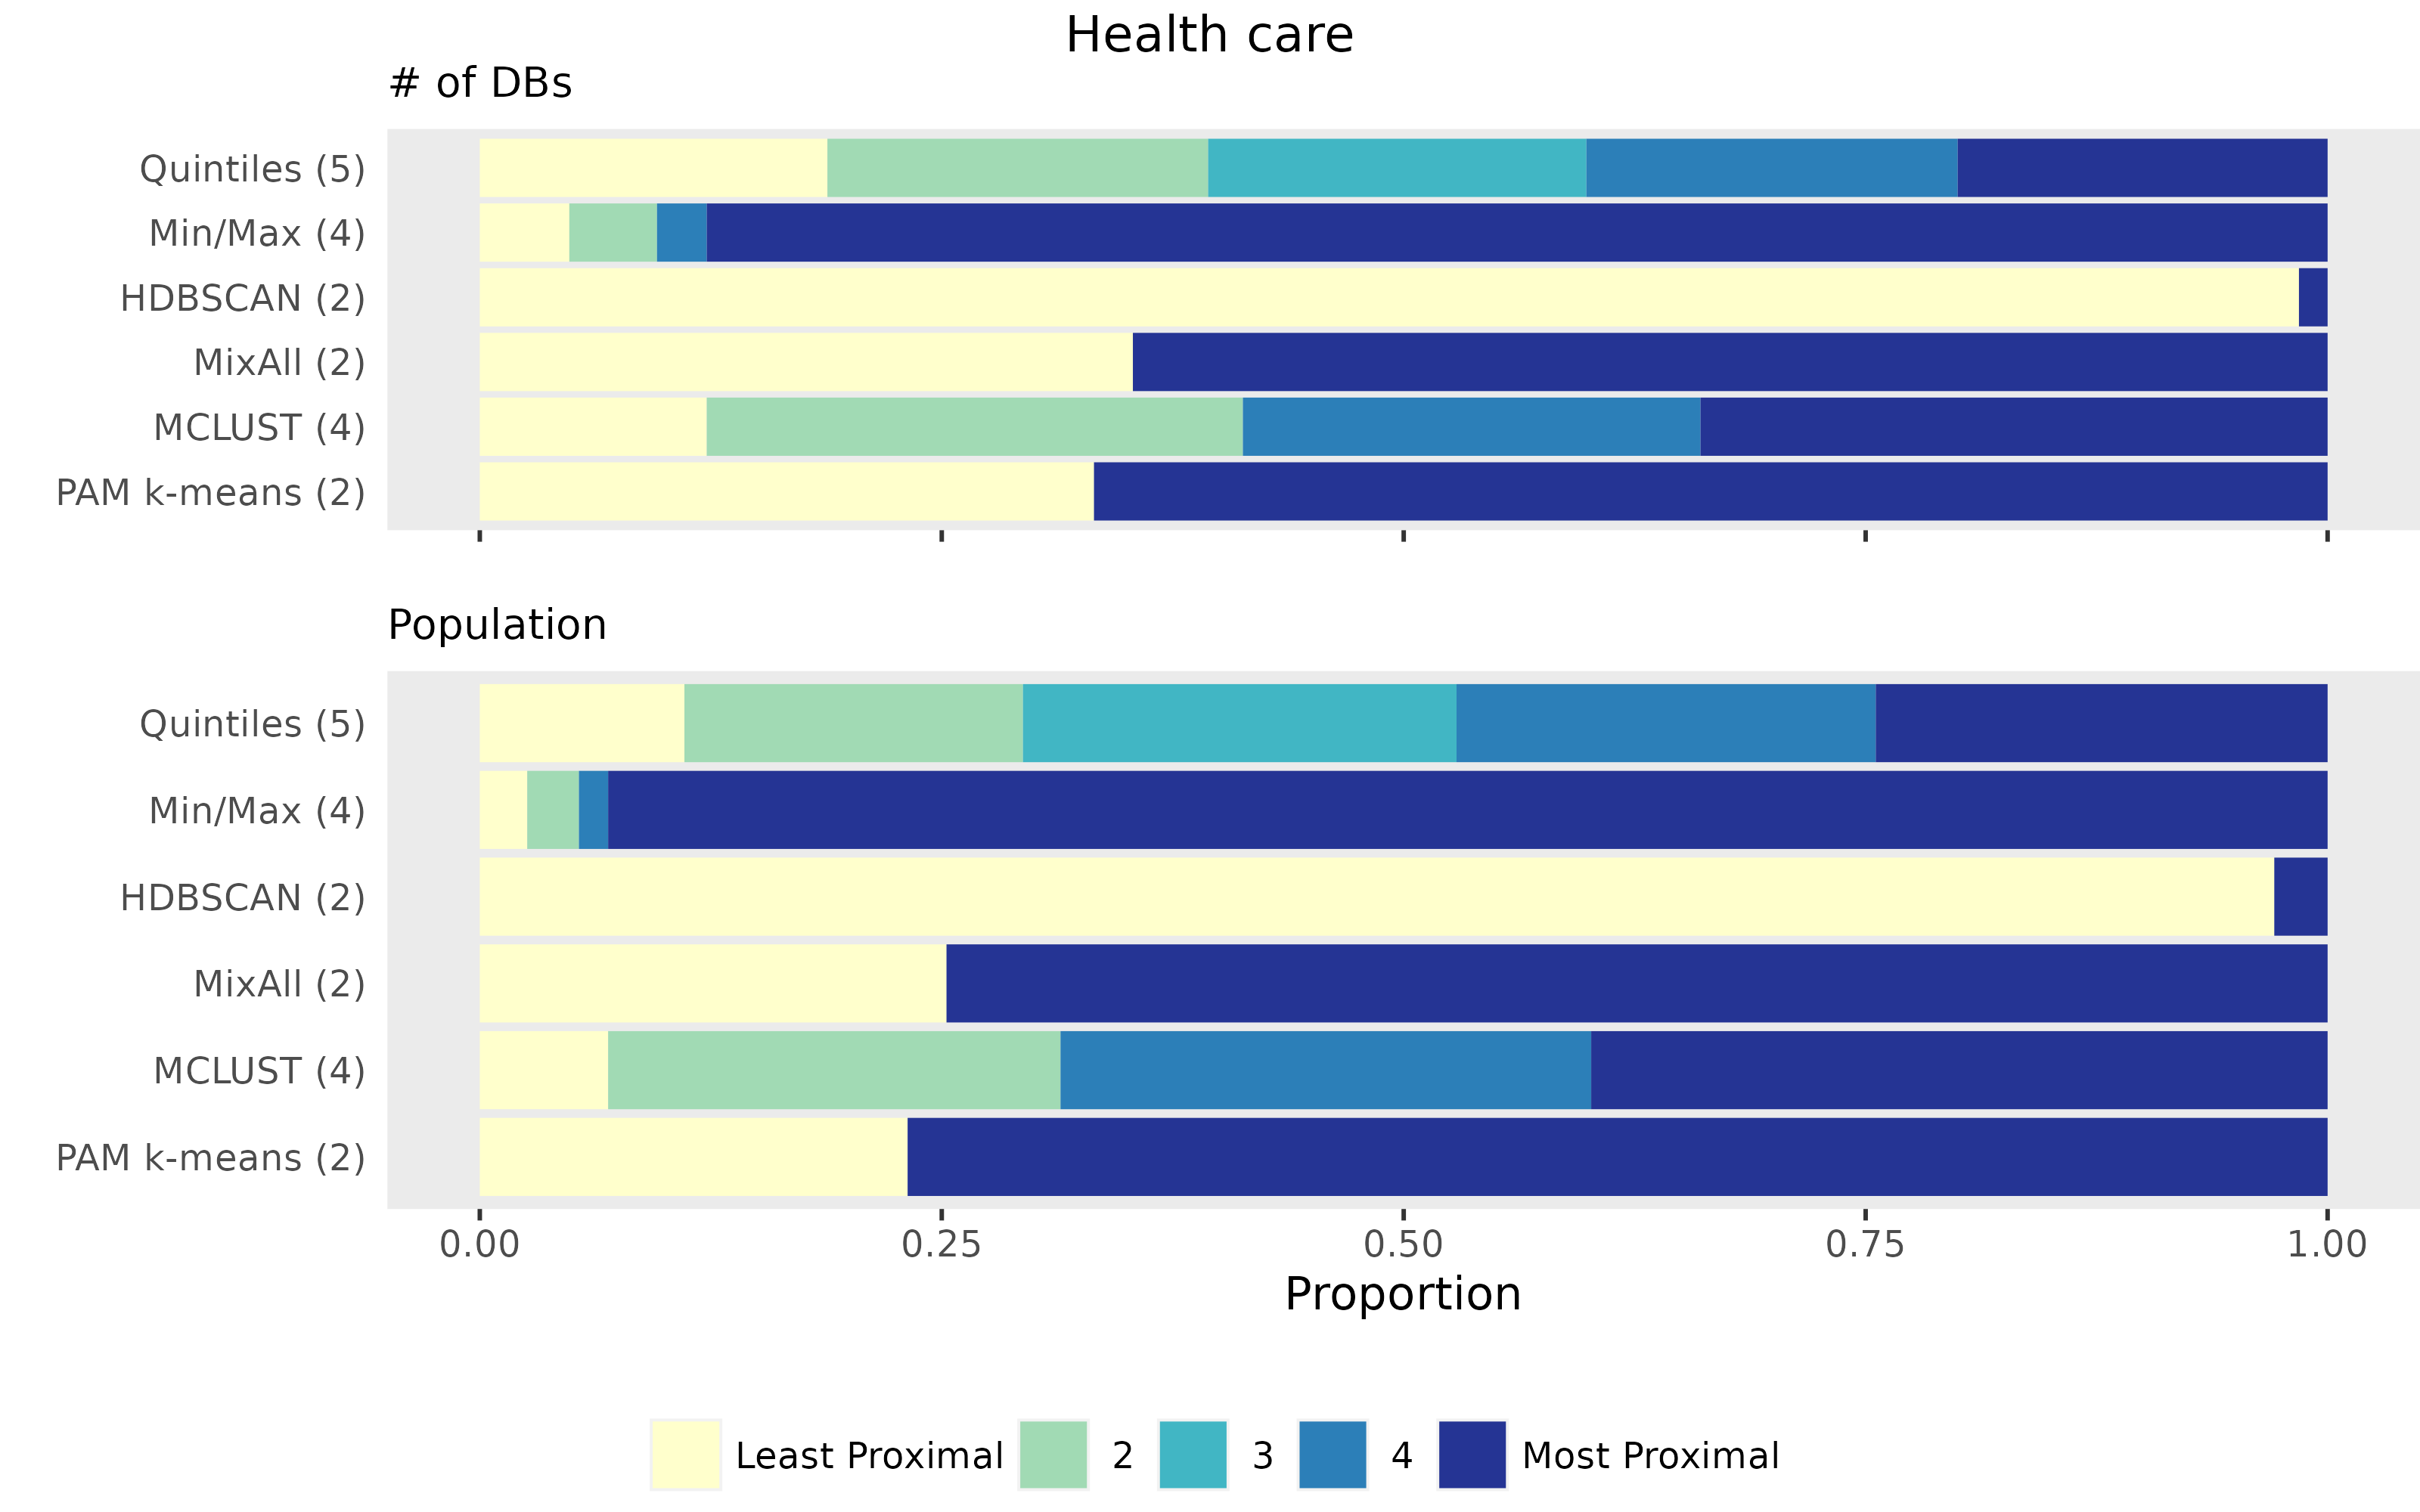
\includegraphics[width=\textwidth]{./barplot_comparison/Health care_barplot.png}
\caption[Health care profile barplot]{Proportion of DBs and population in each cluster for all approaches for the health care amenity.}\label{healthcarebarplot}
\end{figure}









\begin{figure}[H]
\centering
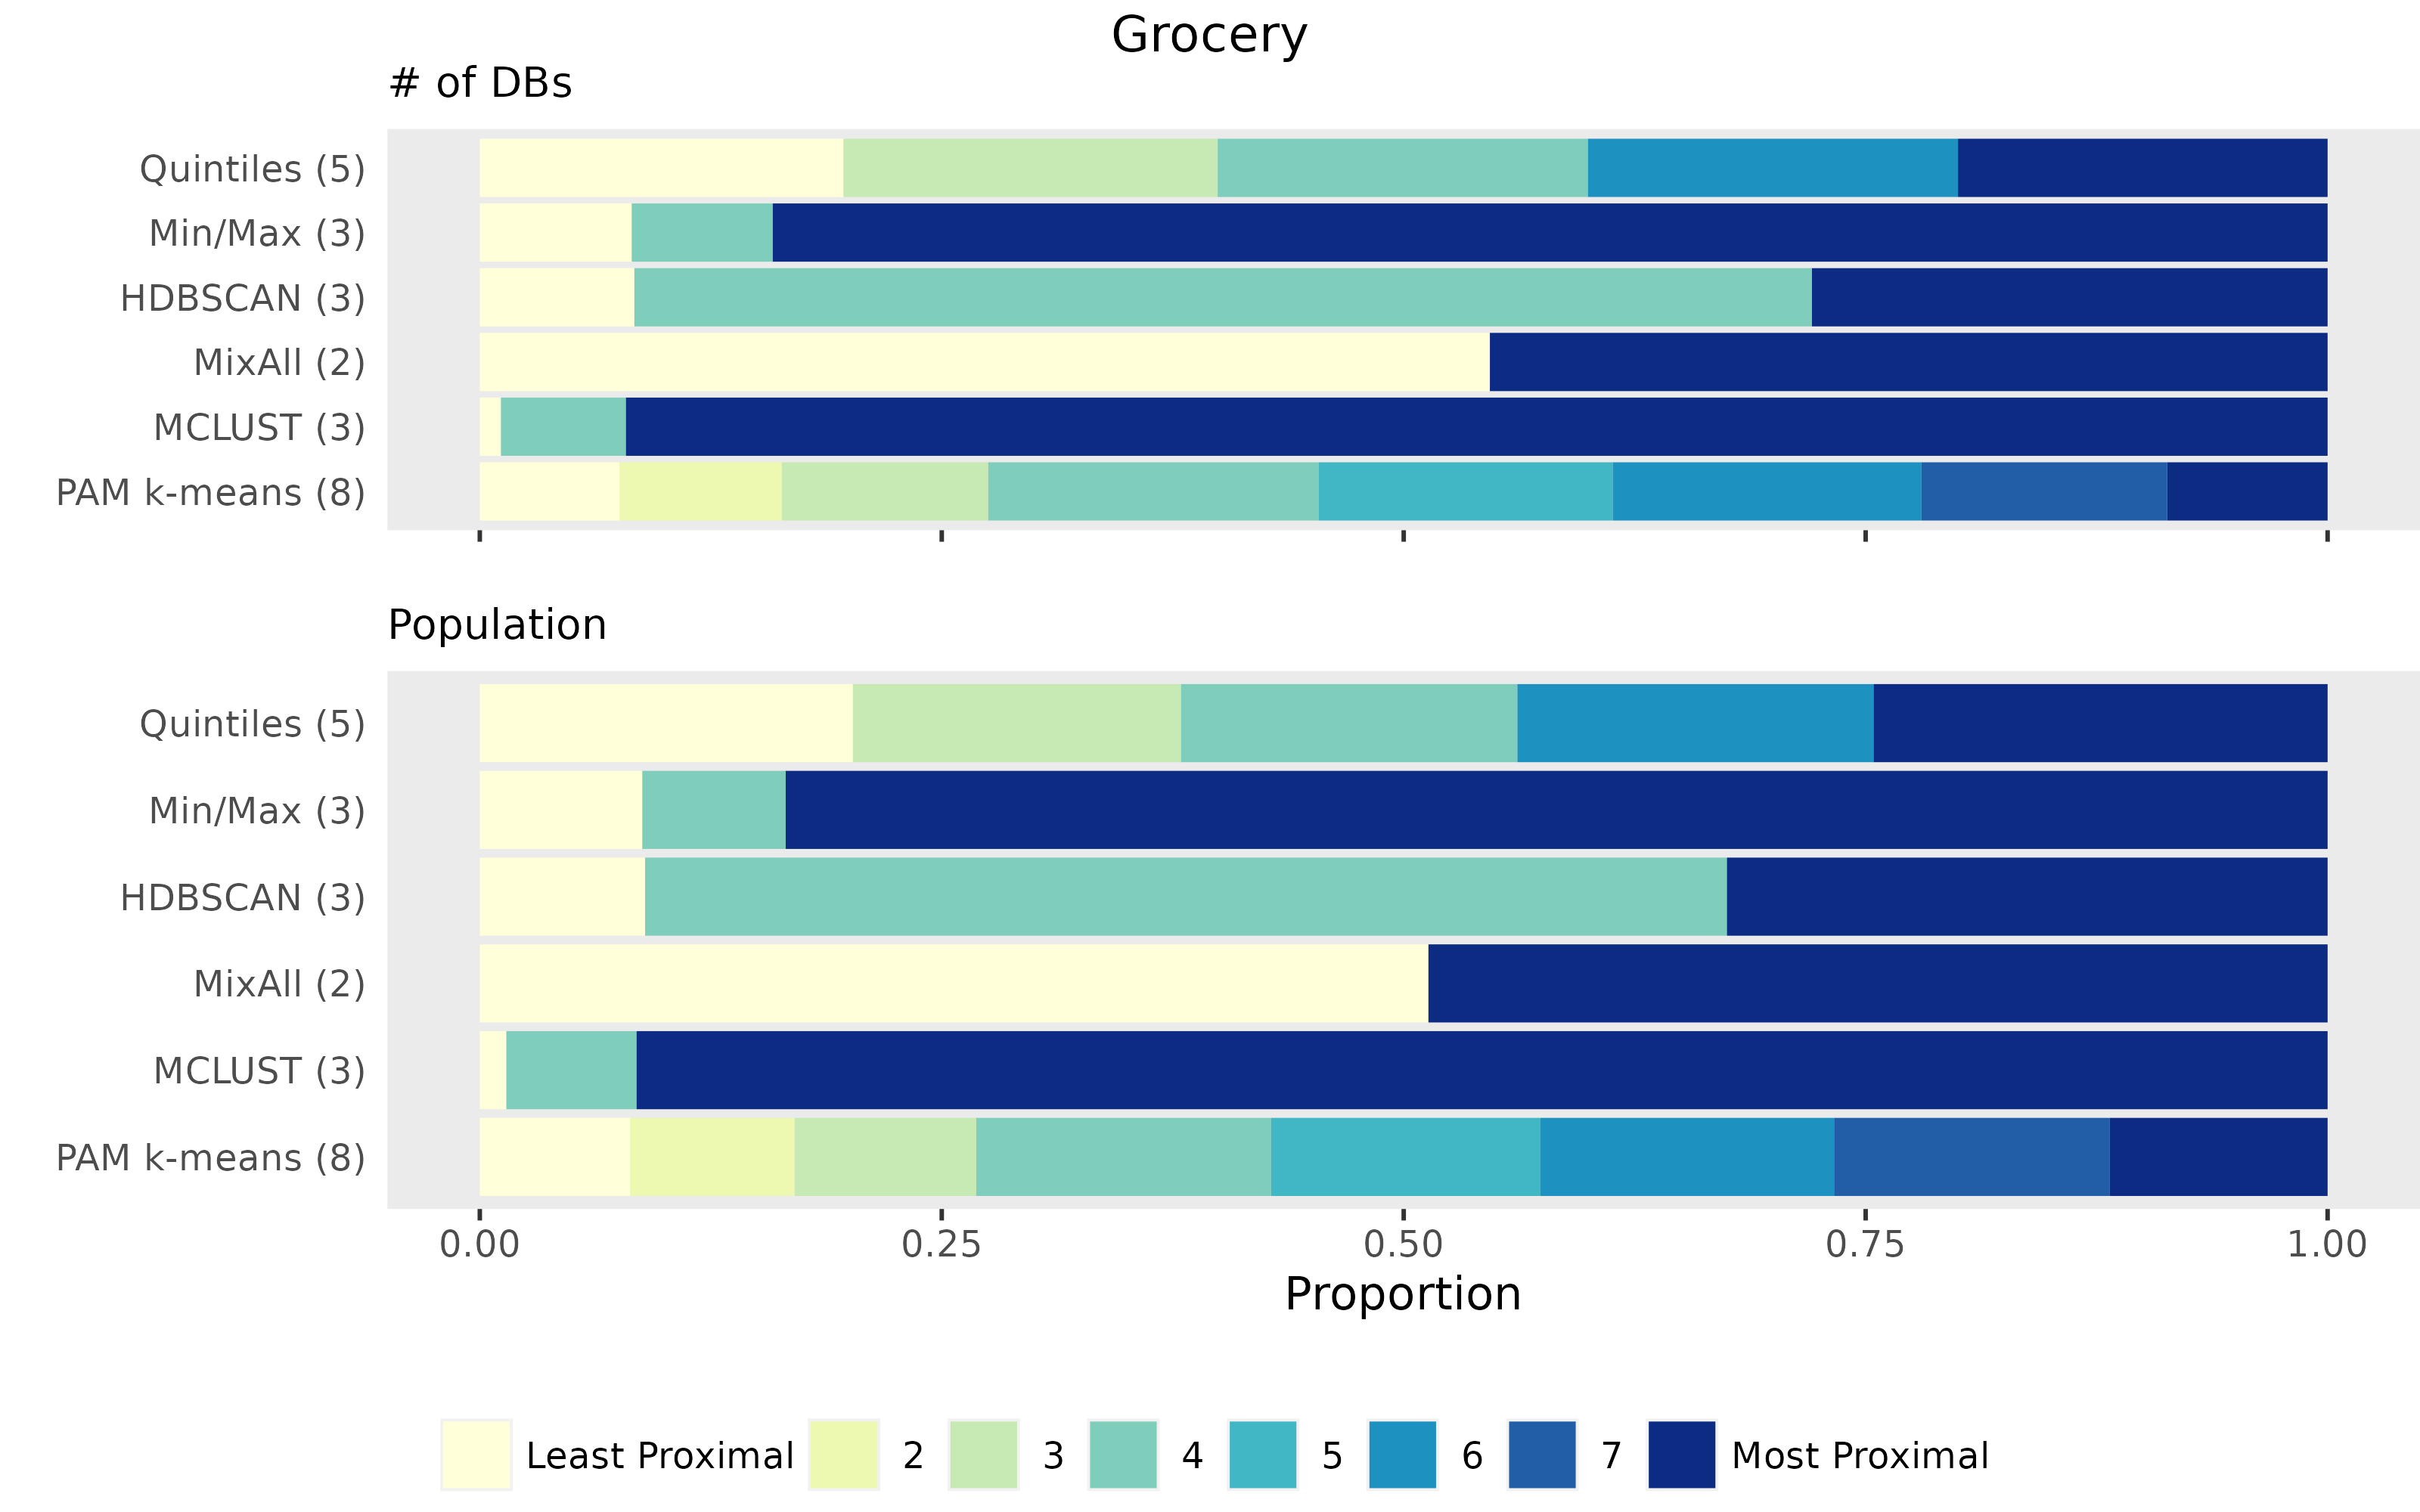
\includegraphics[width=\textwidth]{./barplot_comparison/Grocery_barplot.png}
\caption[Grocery profile barplot]{Proportion of DBs and population in each cluster for all approaches for the grocery amenity.}\label{grocerybarplot}
\end{figure}









\begin{figure}[H]
\centering
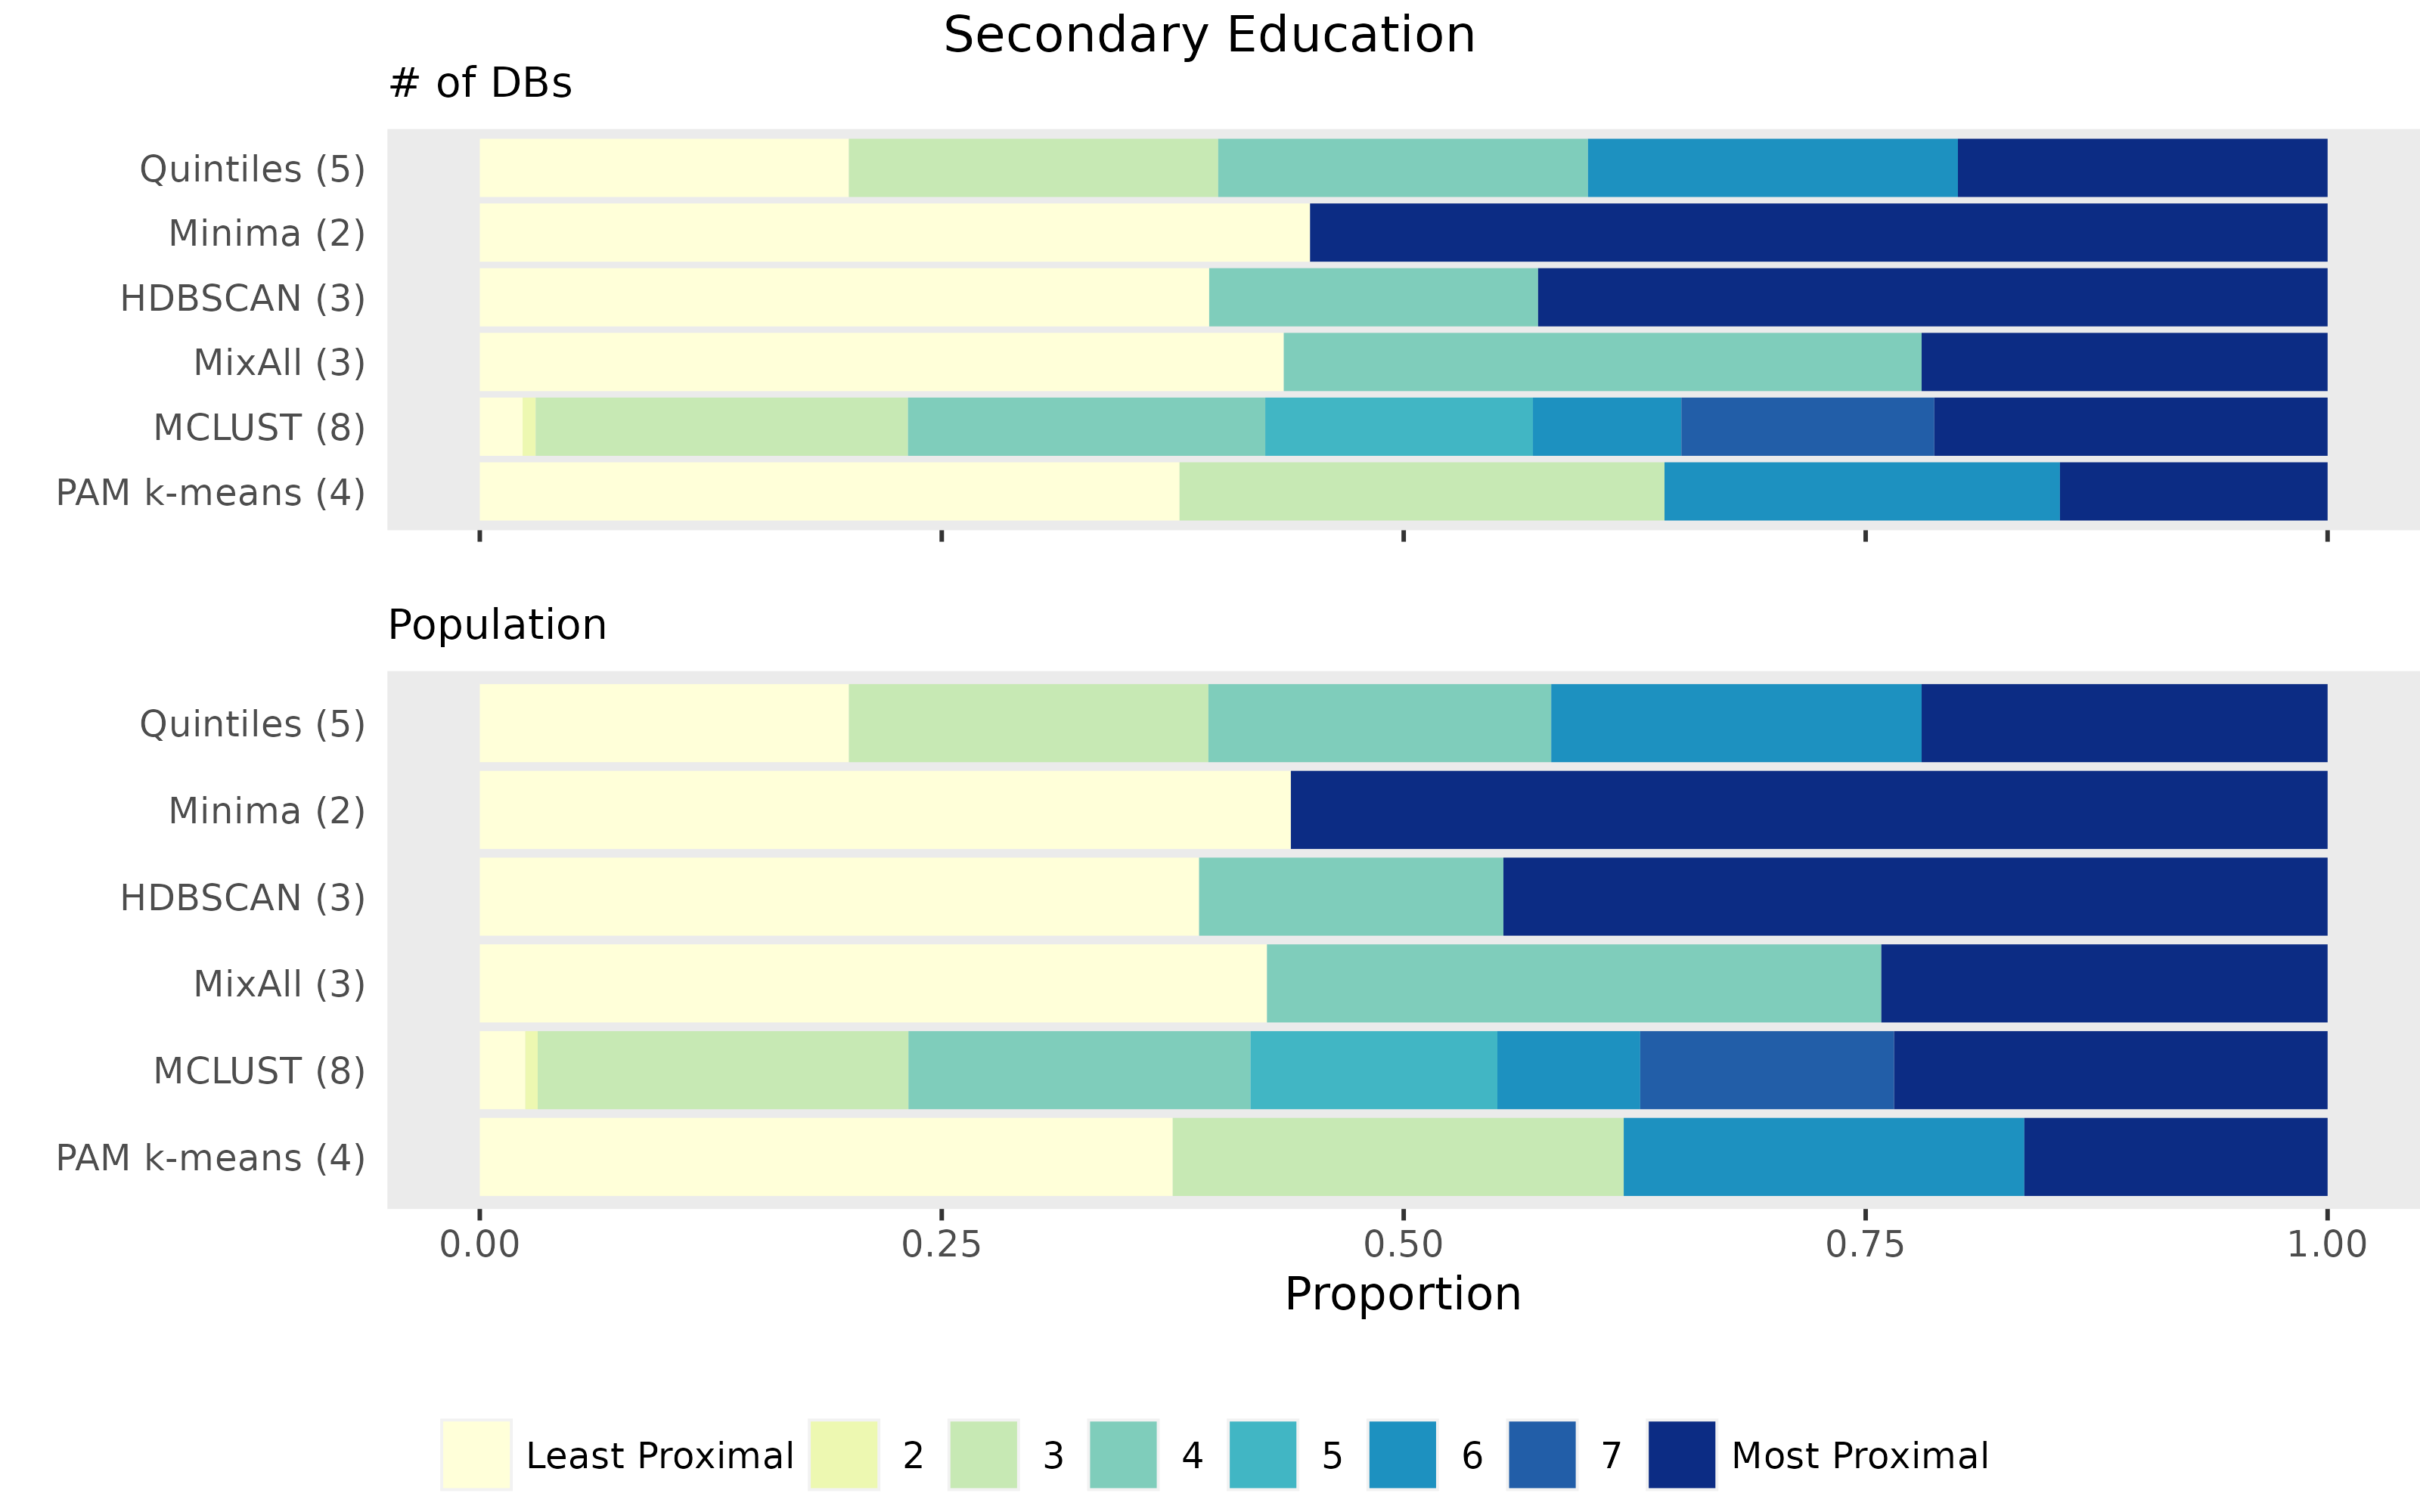
\includegraphics[width=\textwidth]{./barplot_comparison/Secondary Education_barplot.png}
\caption[Secondary education profile barplot]{Proportion of DBs and population in each cluster for all approaches for the secondary education amenity.}\label{seceducbarplot}
\end{figure}









\begin{figure}[H]
\centering
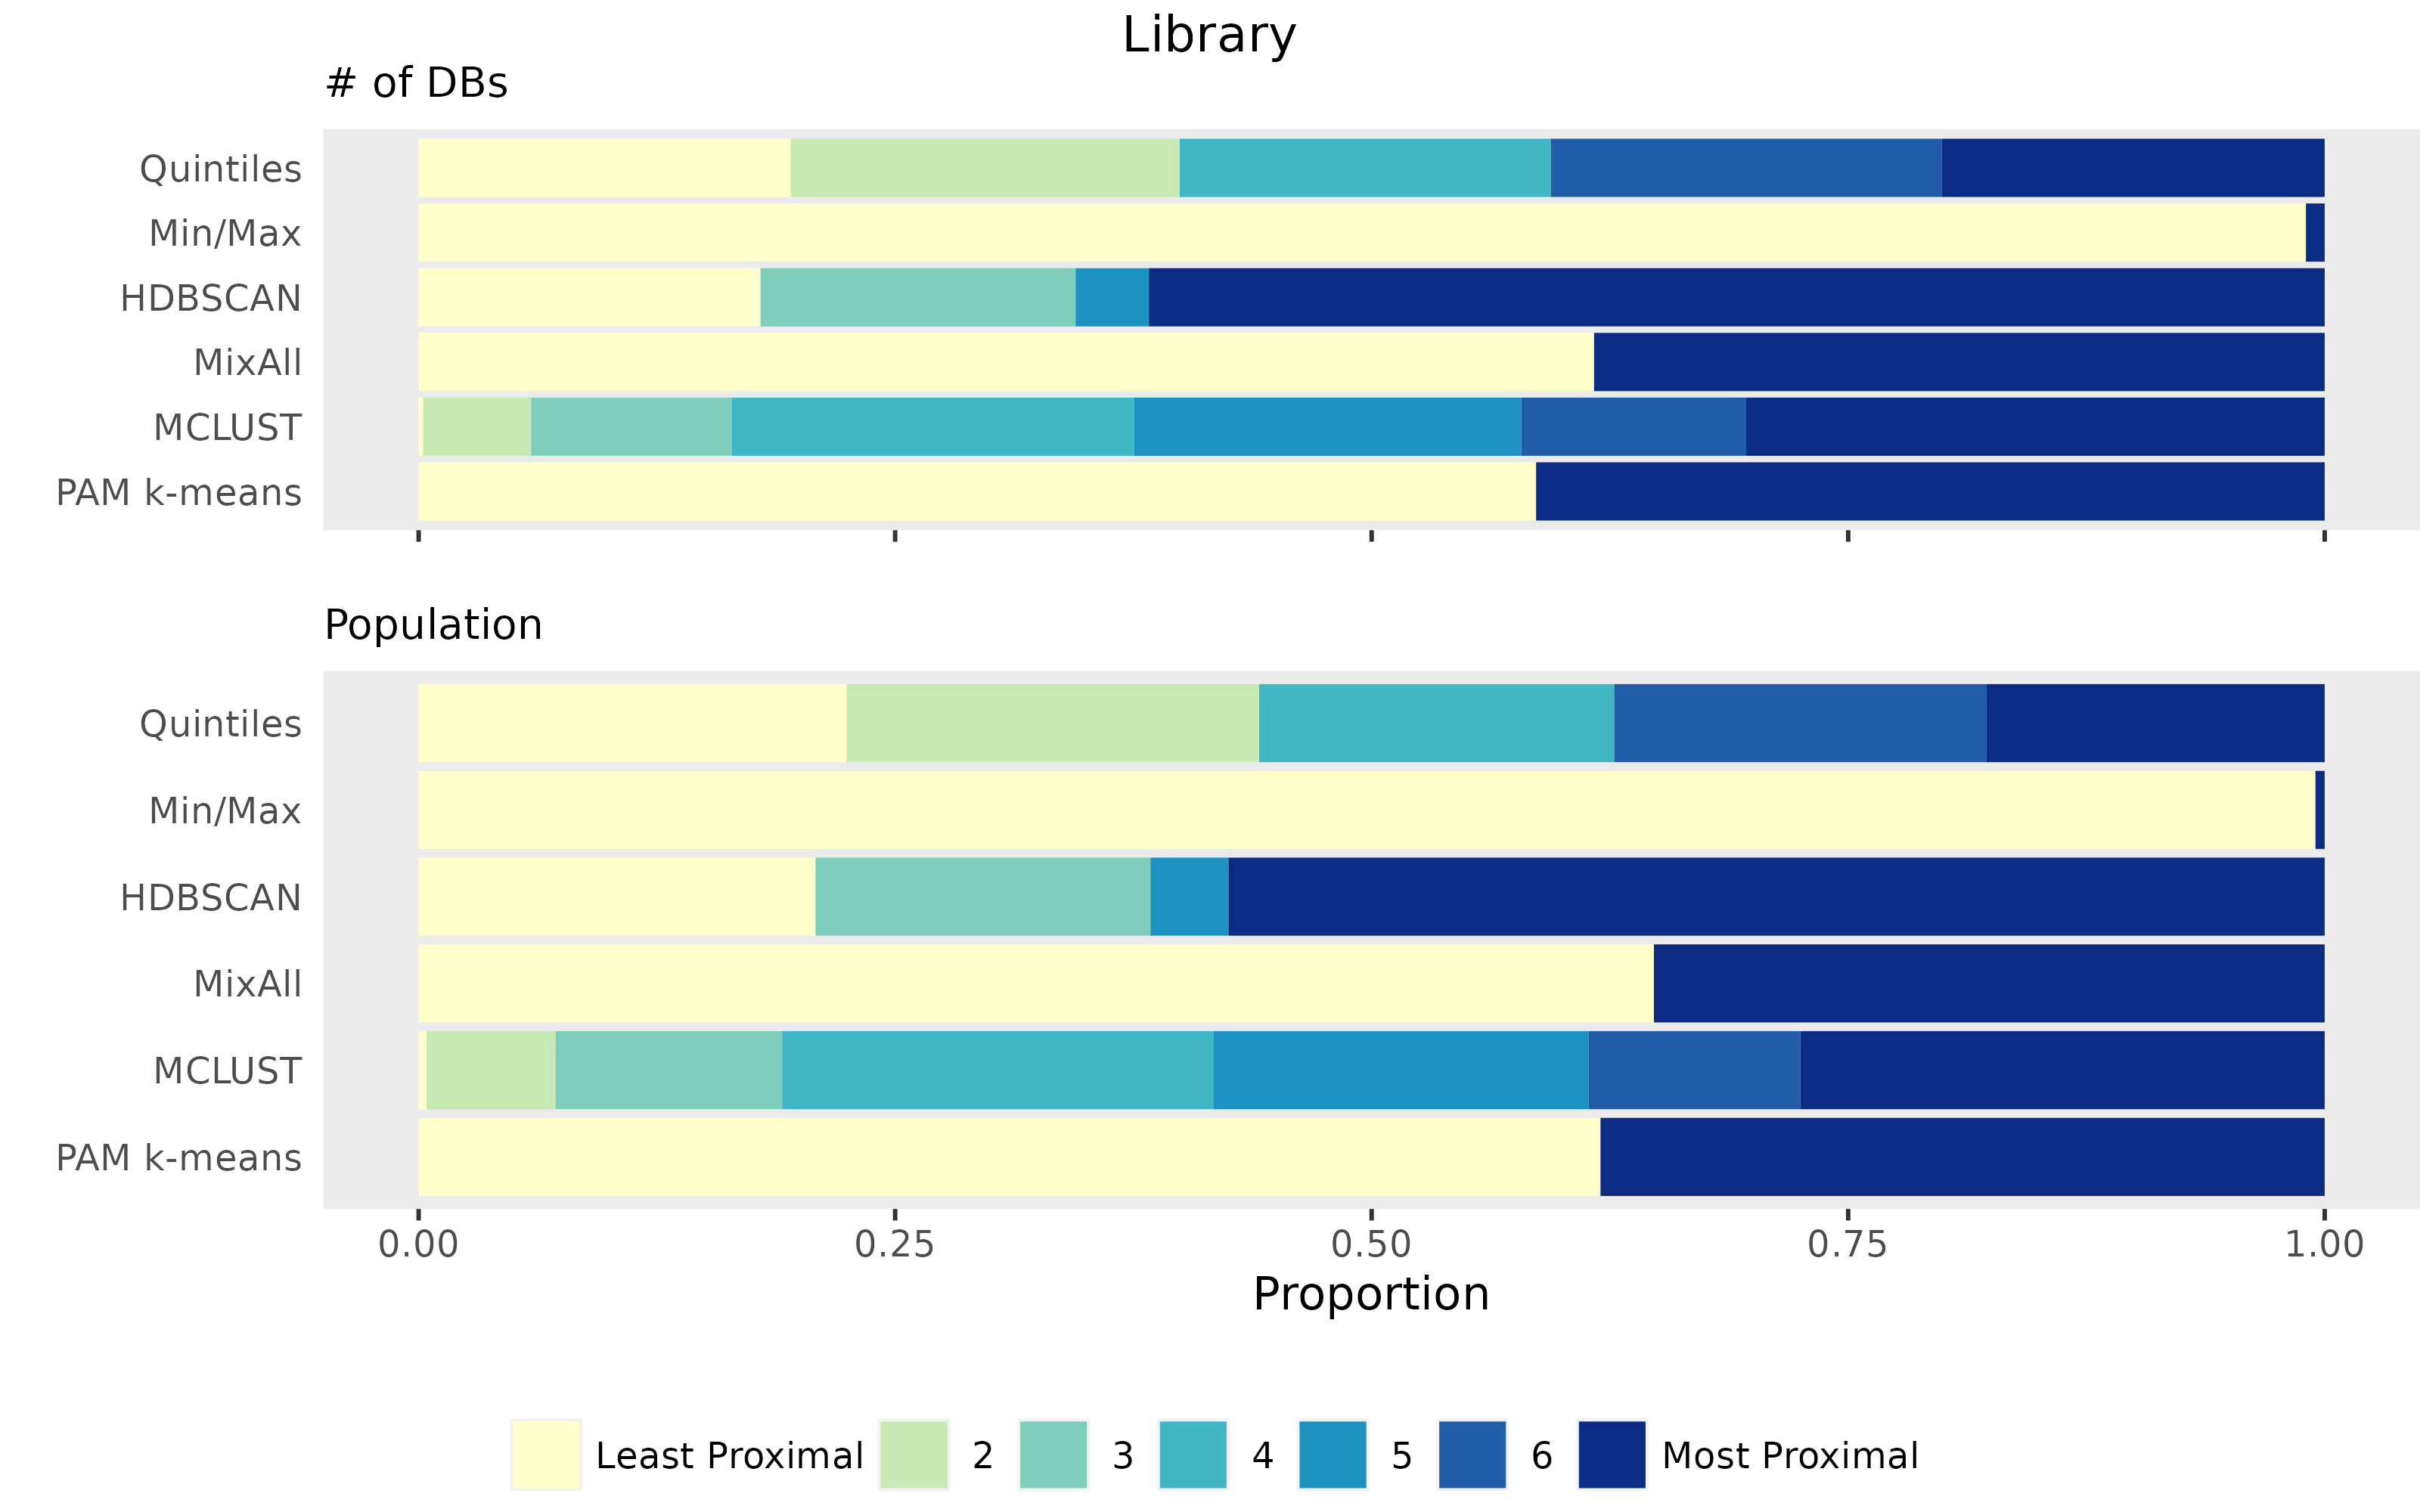
\includegraphics[width=\textwidth]{./barplot_comparison/Library_barplot.png}
\caption[Library profile barplot]{Proportion of DBs and population in each cluster for all approaches for the library amenity.}\label{librarybarplot}
\end{figure}









\begin{figure}[H]
\centering
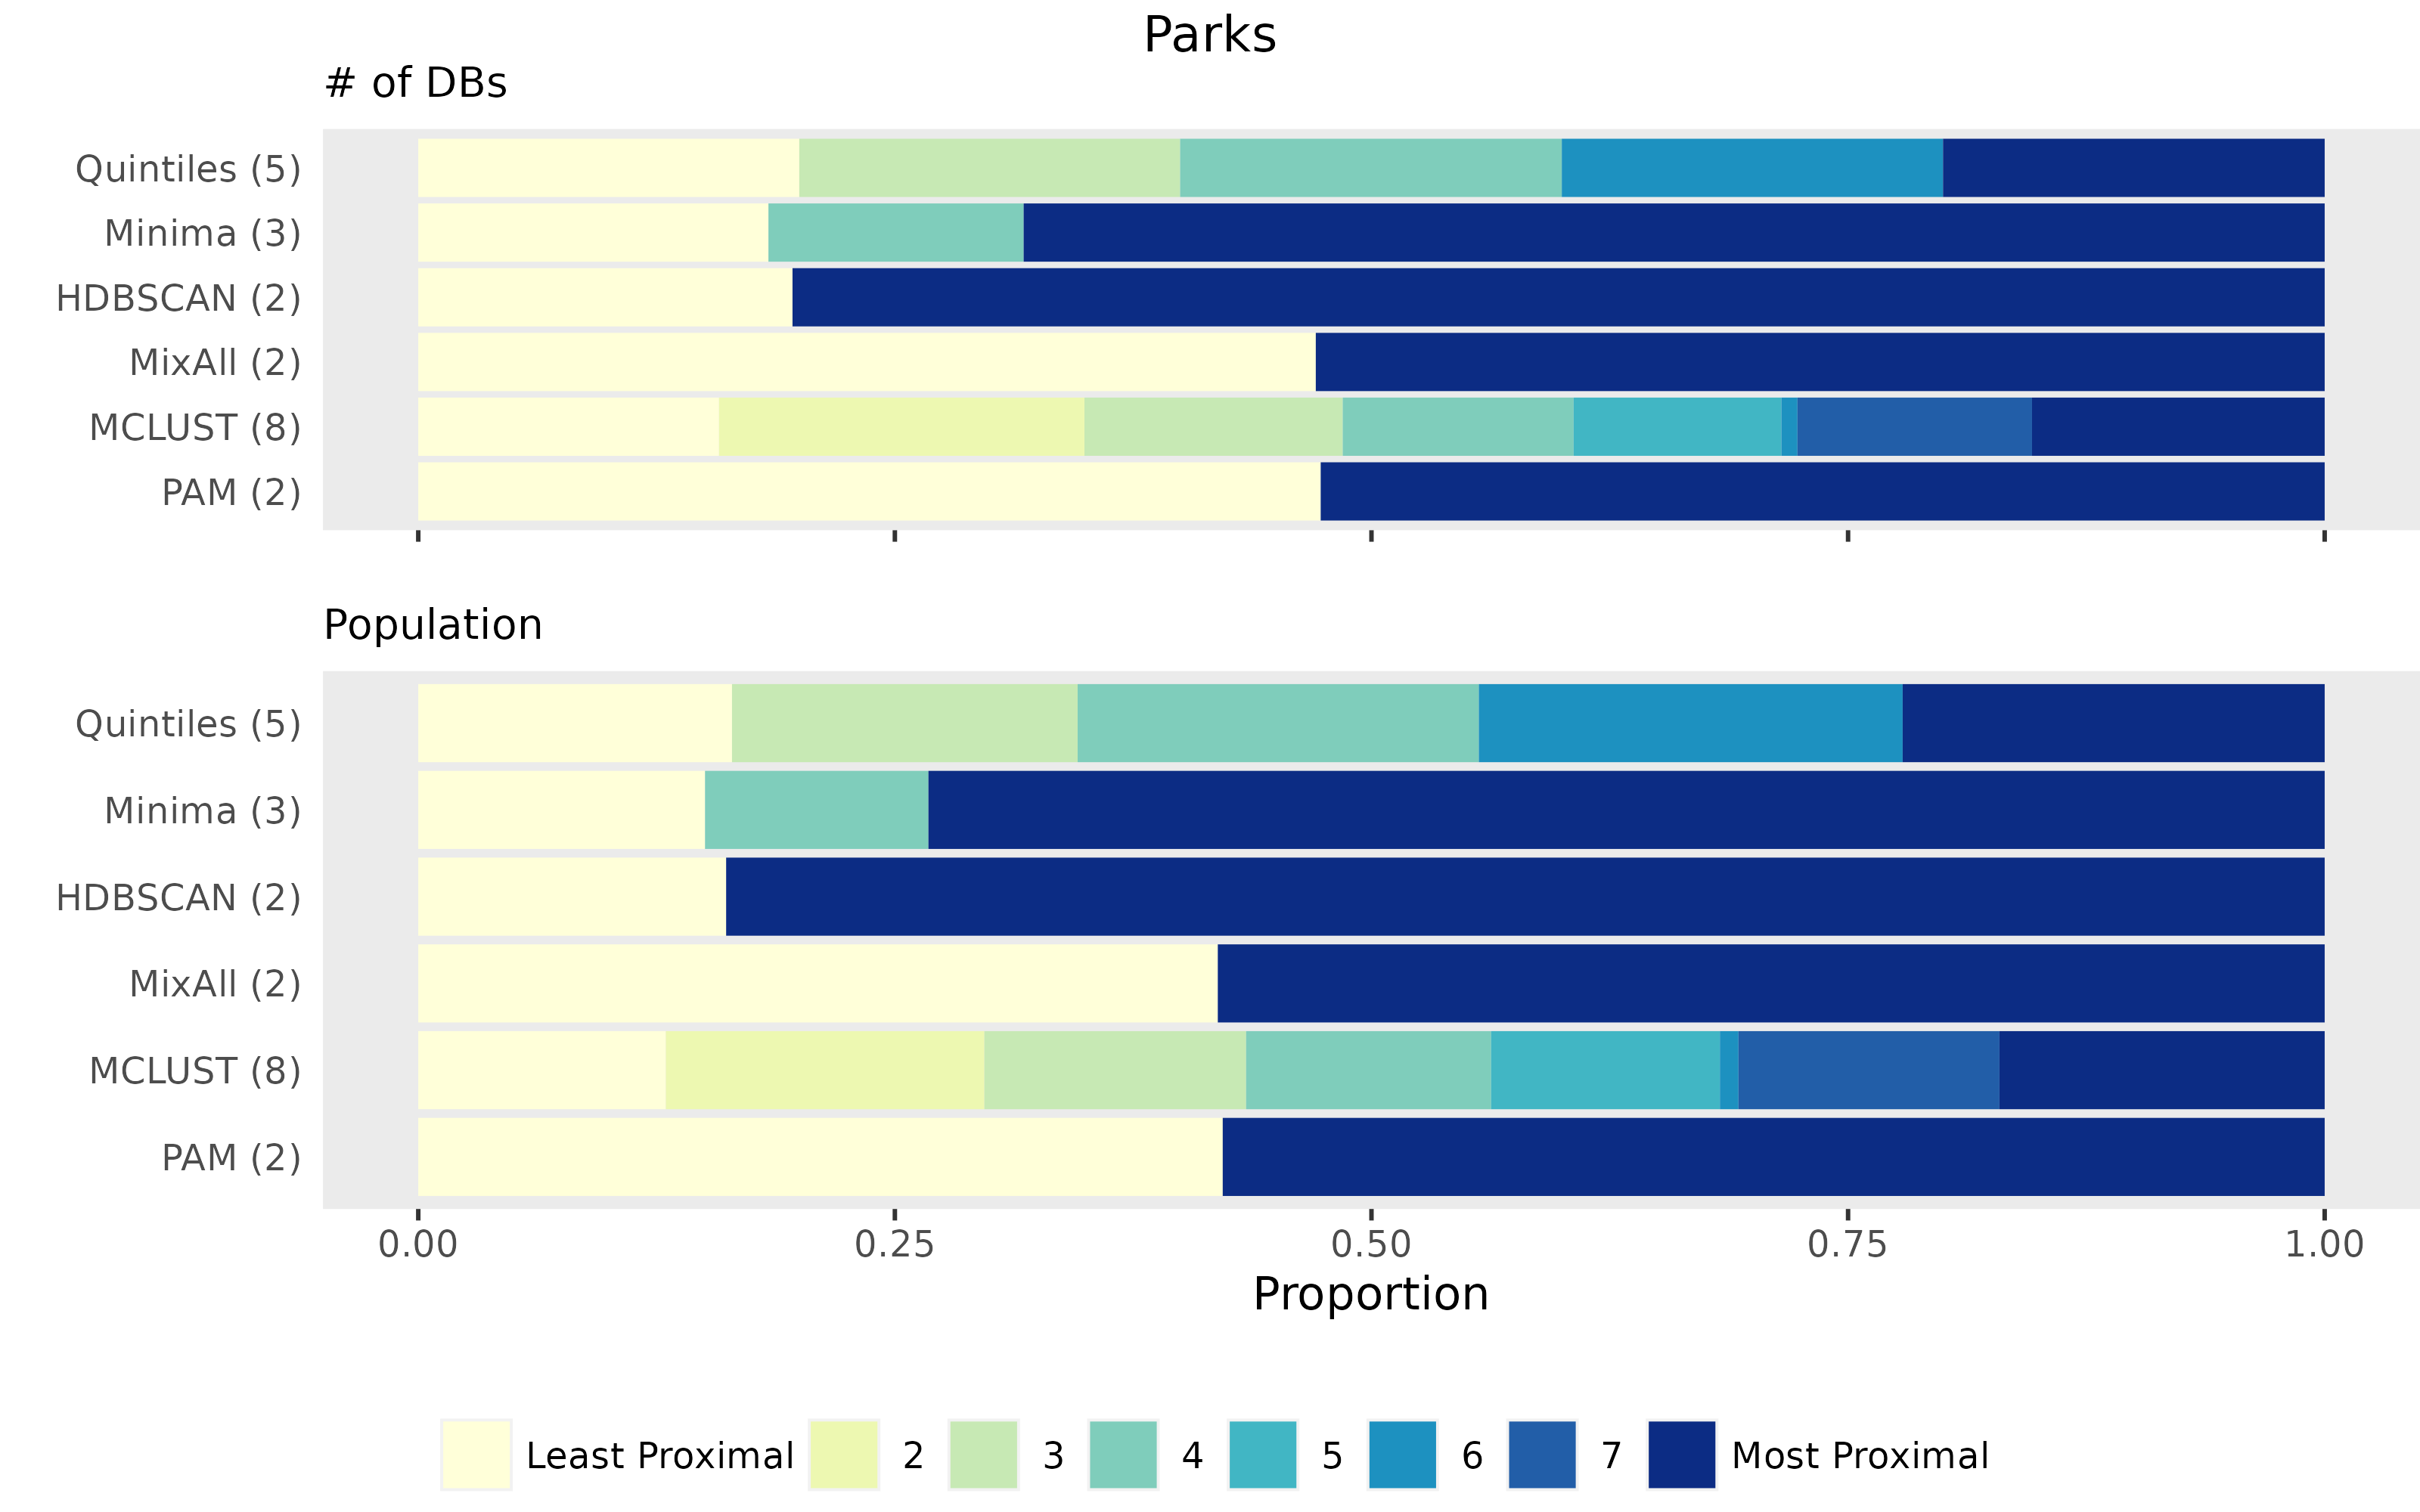
\includegraphics[width=\textwidth]{./barplot_comparison/Parks_barplot.png}
\caption[Parks profile barplot]{Proportion of DBs and population in each cluster for all approaches for the parks amenity.}\label{parksbarplot}
\end{figure}









\begin{figure}[H]
\centering
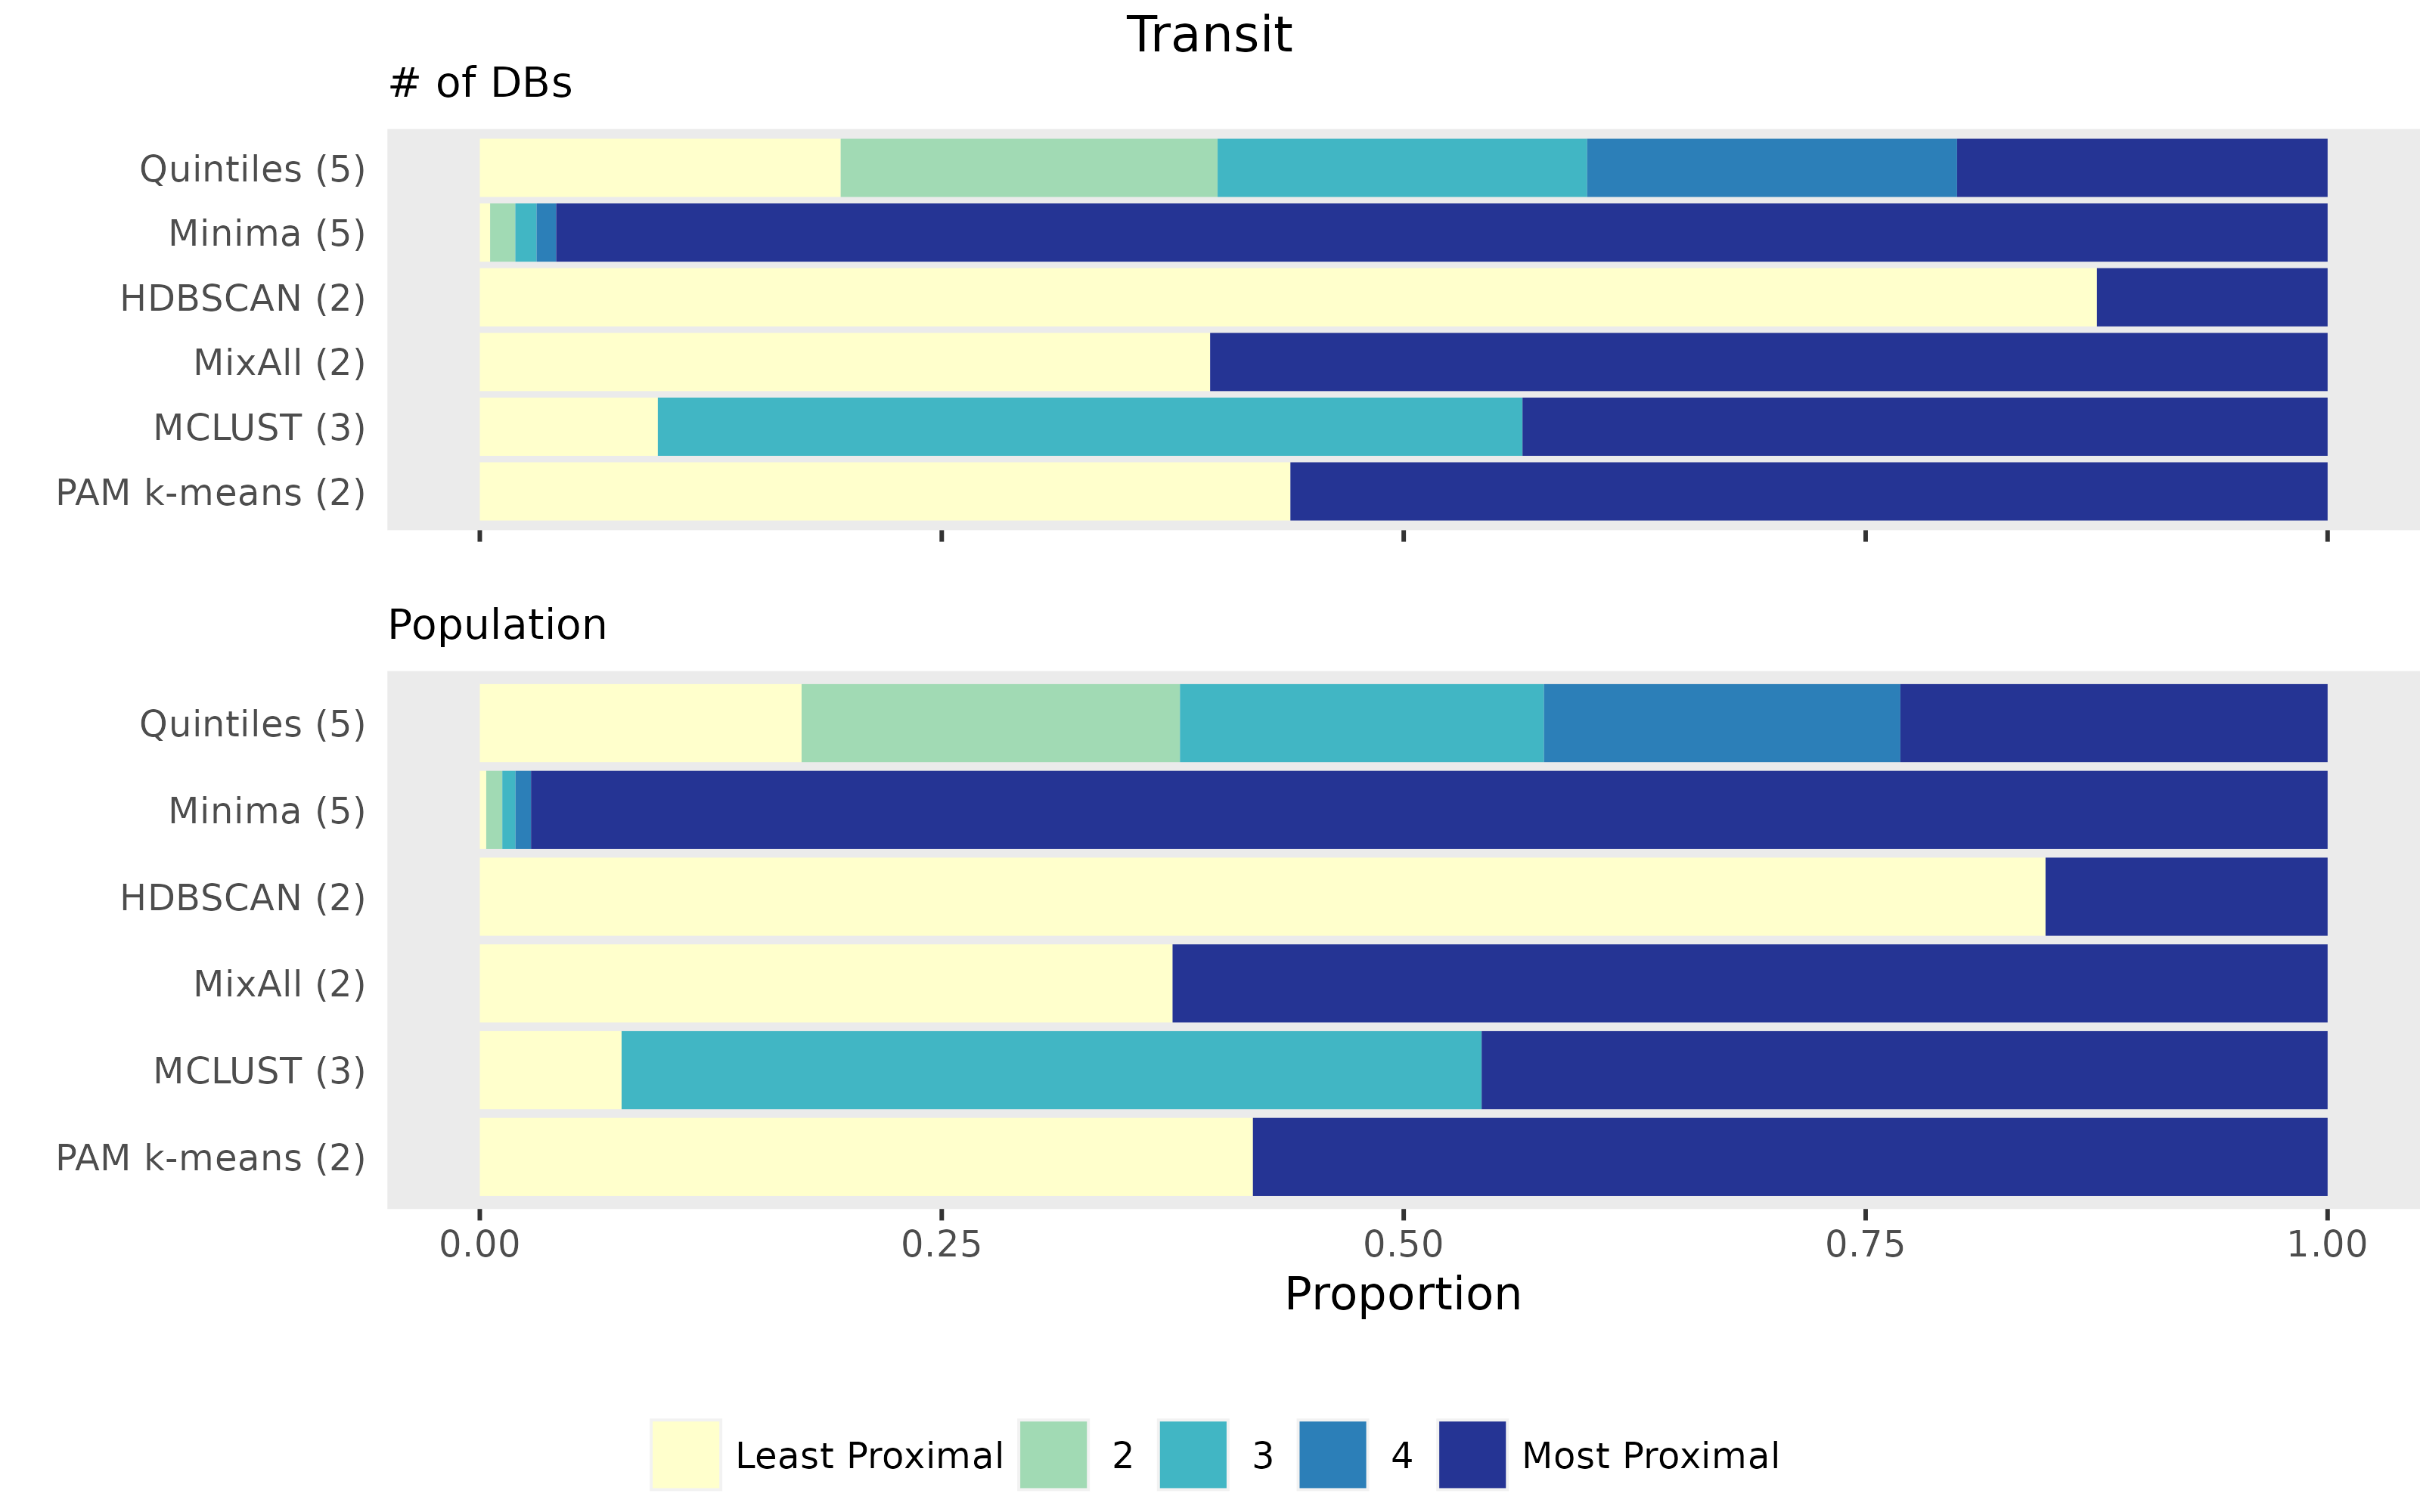
\includegraphics[width=\textwidth]{./barplot_comparison/Transit_barplot.png}
\caption[Transit profile barplot]{Proportion of DBs and population in each cluster for all approaches for the transit amenity.}\label{transitbarplot}
\end{figure}



















\begin{table}[H]
\centering
\resizebox{\textwidth}{!}{
\begin{tabular}{|r|llllllll|}
  \hline
 & \# of DBs & DB Population & Median IoR & CMA Type & Province & Amenity Dense & Employment & Range \\ 
  \hline
Entire Population & 423,602 (100.0\%) & 38 & 0.16 & CMA (48.3\%) & Ontario (18.2\%) & Low (90.1\%) & 0.006 & 0 - 1 \\ 
  Quintiles C1 & 78,014 (18.4\%) & 10 & 0.29 & None (80.9\%) & NovaScotia (6.5\%) & Low (100.0\%) & 0.000 & 0 - 4e-04 \\ 
  Min/Max C1 & 29,831 (7.0\%) & 5 & 0.32 & None (83.6\%) & NovaScotia (8.8\%) & Low (100.0\%) & 0.000 & 0 - 0.0000 \\ 
  HDBSCAN C1 & 419,062 (98.9\%) & 38 & 0.16 & CMA (47.7\%) & Ontario (17.9\%) & Low (90.9\%) & 0.006 & 0 - 0.2298 \\ 
  MixAll C1 & 179,334 (42.3\%) & 16 & 0.27 & None (73.6\%) & Ontario (7.2\%) & Low (99.9\%) & 0.000 & 0 - 0.0036 \\ 
  MCLUST C1 & 29,831 (7.0\%) & 5 & 0.32 & None (83.6\%) & NovaScotia (8.8\%) & Low (100.0\%) & 0.000 & 0 - 0.0000 \\ 
  PAM k-means C1 & 177,804 (42.0\%) & 16 & 0.27 & None (73.8\%) & Ontario (7.1\%) & Low (99.9\%) & 0.000 & 0 - 0.0035 \\ 
  Quintiles C2 & 89,705 (21.2\%) & 23 & 0.24 & None (69.6\%) & Ontario (9.2\%) & Low (99.9\%) & 0.001 & 4e-04 - 0.0030 \\ 
  Min/Max C2 & 22,179 (5.2\%) & 10 & 0.30 & None (81.2\%) & NovaScotia (5.6\%) & Low (100.0\%) & 0.000 & 0.0000 - 2e-04 \\ 
  HDBSCAN C2 & 4,540 (1.1\%) & 122 & 0.03 & CMA (100.0\%) & Ontario (44.9\%) & Med (45.9\%) & 0.292 & 0.2298 - 1 \\ 
  MixAll C2 & 244,268 (57.7\%) & 63 & 0.11 & CMA (73.3\%) & Ontario (26.3\%) & Low (82.8\%) & 0.023 & 0.0036 - 1 \\ 
  MCLUST C2 & 56,902 (13.4\%) & 10 & 0.27 & None (78.6\%) & Ontario (6.3\%) & Low (100.0\%) & 0.000 & 0.0000 - 4e-04 \\ 
  PAM k-means C2 & 245,798 (58.0\%) & 62 & 0.11 & CMA (73.0\%) & Ontario (26.2\%) & Low (82.9\%) & 0.023 & 0.0035 - 1 \\ 
  Quintiles C3 & 85,928 (20.3\%) & 41 & 0.20 & CMA (34.2\%) & Ontario (12.7\%) & Low (97.8\%) & 0.006 & 0.0030 - 0.0127 \\ 
  Min/Max C3 & 14,893 (3.5\%) & 10 & 0.27 & None (78.3\%) & Ontario (6.7\%) & Low (100.0\%) & 0.000 & 2e-04 - 3e-04 \\ 
  MCLUST C3 & 39,730 (9.4\%) & 20 & 0.24 & None (72.7\%) & Ontario (9.4\%) & Low (99.9\%) & 0.001 & 4e-04 - 0.0012 \\ 
  Quintiles C4 & 85,096 (20.1\%) & 65 & 0.11 & CMA (79.7\%) & Ontario (26.9\%) & Low (89.9\%) & 0.022 & 0.0127 - 0.0368 \\ 
  Min/Max C4 & 26,887 (6.3\%) & 17 & 0.23 & None (75.4\%) & Ontario (8.6\%) & Low (100.0\%) & 0.000 & 3e-04 - 5e-04 \\ 
  MCLUST C4 & 48,188 (11.4\%) & 27 & 0.25 & None (64.2\%) & Ontario (9.3\%) & Low (99.7\%) & 0.002 & 0.0012 - 0.0033 \\ 
  Quintiles C5 & 84,859 (20.0\%) & 83 & 0.06 & CMA (99.5\%) & Ontario (37.2\%) & Low (62.8\%) & 0.072 & 0.0368 - 1 \\ 
  Min/Max C5 & 329,812 (77.9\%) & 50 & 0.14 & CMA (59.1\%) & Ontario (21.9\%) & Low (87.2\%) & 0.014 & 5e-04 - 1 \\ 
  MCLUST C5 & 53,628 (12.7\%) & 38 & 0.21 & None (37.2\%) & Ontario (11.3\%) & Low (98.5\%) & 0.005 & 0.0033 - 0.0085 \\ 
  MCLUST C6 & 64,056 (15.1\%) & 57 & 0.14 & CMA (61.2\%) & Ontario (19.1\%) & Low (93.8\%) & 0.014 & 0.0085 - 0.0206 \\ 
  MCLUST C7 & 69,082 (16.3\%) & 71 & 0.10 & CMA (91.8\%) & Ontario (34.7\%) & Low (85.2\%) & 0.032 & 0.0206 - 0.0518 \\ 
  MCLUST C8 & 51,824 (12.2\%) & 82 & 0.06 & CMA (99.8\%) & Ontario (36.4\%) & Low (63.8\%) & 0.081 & 0.0518 - 0.1629 \\ 
  MCLUST C9 & 10,361 (2.4\%) & 118 & 0.03 & CMA (100.0\%) & Quebec (37.9\%) & Med (46.0\%) & 0.219 & 0.1629 - 1 \\ 
   \hline
\end{tabular}
}
\caption[Employment cluster profiles]{Summary statistics for each cluster found by all approaches for the employment amenity. DB Population, IoR and proximity value show the median, while CMA Type, Province and Amenity Dense show the mode.}\label{employmentprofiles}
\end{table}









\begin{table}[H]
\centering
\resizebox{\textwidth}{!}{
\begin{tabular}{|r|llllllll|}
  \hline
 & \# of DBs & DB Population & Median IoR & CMA Type & Province & Amenity Dense & Pharmacy & Range \\ 
  \hline
Entire Population & 178,521 (100.0\%) & 63 & 0.11 & CMA (71.7\%) & Ontario (27.4\%) & Low (76.4\%) & 0.026 & 0 - 1 \\ 
  Quintiles C1 & 34,980 (19.6\%) & 60 & 0.13 & CMA (64.1\%) & Ontario (21.8\%) & Low (91.5\%) & 0.007 & 0 - 0.0098 \\ 
  Min/Max C1 & 41,305 (23.1\%) & 59 & 0.13 & CMA (63.9\%) & Ontario (22.0\%) & Low (91.6\%) & 0.008 & 0 - 0.0114 \\ 
  HDBSCAN C1 & 42,510 (23.8\%) & 59 & 0.13 & CMA (63.9\%) & Ontario (22.0\%) & Low (91.6\%) & 0.008 & 0 - 0.0118 \\ 
  MixAll C1 & 91,454 (51.2\%) & 60 & 0.12 & CMA (66.7\%) & Ontario (24.1\%) & Low (88.6\%) & 0.013 & 0 - 0.0265 \\ 
  MCLUST C1 & 3,222 (1.8\%) & 70 & 0.14 & CMA (60.5\%) & Ontario (20.7\%) & Low (93.5\%) & 0.006 & 0 - 0.0064 \\ 
  PAM k-means C1 & 90,986 (51.0\%) & 60 & 0.12 & CMA (66.6\%) & Ontario (24.1\%) & Low (88.7\%) & 0.013 & 0 - 0.0263 \\ 
  Quintiles C2 & 36,365 (20.4\%) & 60 & 0.12 & CMA (66.8\%) & Ontario (24.4\%) & Low (88.7\%) & 0.014 & 0.0098 - 0.0193 \\ 
  Min/Max C2 & 30,505 (17.1\%) & 60 & 0.11 & CMA (67.7\%) & Ontario (24.7\%) & Low (87.9\%) & 0.015 & 0.0114 - 0.0195 \\ 
  HDBSCAN C2 & 90,111 (50.5\%) & 63 & 0.11 & CMA (71.5\%) & Ontario (27.9\%) & Low (81.2\%) & 0.025 & 0.0118 - 0.0525 \\ 
  MixAll C2 & 87,067 (48.8\%) & 67 & 0.10 & CMA (77.0\%) & Ontario (30.9\%) & Low (63.6\%) & 0.055 & 0.0265 - 1 \\ 
  MCLUST C2 & 35,979 (20.2\%) & 59 & 0.13 & CMA (64.3\%) & Ontario (22.0\%) & Low (91.4\%) & 0.008 & 0.0064 - 0.0108 \\ 
  PAM k-means C2 & 87,535 (49.0\%) & 67 & 0.10 & CMA (77.0\%) & Ontario (30.9\%) & Low (63.7\%) & 0.055 & 0.0263 - 1 \\ 
  Quintiles C3 & 35,730 (20.0\%) & 63 & 0.11 & CMA (72.1\%) & Ontario (28.5\%) & Low (81.3\%) & 0.026 & 0.0193 - 0.0341 \\ 
  Min/Max C3 & 106,711 (59.8\%) & 66 & 0.11 & CMA (75.8\%) & Ontario (30.3\%) & Low (67.2\%) & 0.046 & 0.0195 - 1 \\ 
  HDBSCAN C3 & 45,900 (25.7\%) & 70 & 0.09 & CMA (79.2\%) & Ontario (31.5\%) & Low (52.9\%) & 0.085 & 0.0525 - 1 \\ 
  MCLUST C3 & 2,075 (1.2\%) & 56 & 0.13 & CMA (61.8\%) & Ontario (23.1\%) & Low (92.8\%) & 0.011 & 0.0108 - 0.0114 \\ 
  Quintiles C4 & 35,697 (20.0\%) & 66 & 0.11 & CMA (75.0\%) & Ontario (30.9\%) & Low (72.0\%) & 0.046 & 0.0341 - 0.0641 \\ 
  MCLUST C4 & 26,864 (15.0\%) & 60 & 0.11 & CMA (67.5\%) & Ontario (24.7\%) & Low (88.1\%) & 0.015 & 0.0114 - 0.0181 \\ 
  Quintiles C5 & 35,749 (20.0\%) & 71 & 0.08 & CMA (80.3\%) & Ontario (31.6\%) & Low (48.5\%) & 0.098 & 0.0641 - 1 \\ 
  MCLUST C5 & 37,376 (20.9\%) & 62 & 0.11 & CMA (71.8\%) & Ontario (28.1\%) & Low (82.0\%) & 0.025 & 0.0181 - 0.0332 \\ 
  MCLUST C6 & 30,077 (16.8\%) & 65 & 0.11 & CMA (74.9\%) & Ontario (30.8\%) & Low (73.1\%) & 0.042 & 0.0332 - 0.0554 \\ 
  MCLUST C7 & 42,928 (24.0\%) & 70 & 0.09 & CMA (79.5\%) & Ontario (31.5\%) & Low (51.8\%) & 0.088 & 0.0554 - 1 \\ 
   \hline
\end{tabular}
}
\caption[Pharmacy cluster profiles]{Summary statistics for each cluster found by all approaches for the pharmacy amenity. DB Population, IoR and proximity value show the median, while CMA Type, Province and Amenity Dense show the mode.}\label{pharmacyprofiles}
\end{table}










\begin{table}[H]
\centering
\resizebox{\textwidth}{!}{
\begin{tabular}{|r|llllllll|}
  \hline
 & \# of DBs & DB Population & Median IoR & CMA Type & Province & Amenity Dense & Childcare & Range \\ 
  \hline
Entire Population & 243,964 (100.0\%) & 62 & 0.11 & CMA (68.3\%) & Ontario (23.9\%) & Low (82.7\%) & 0.048 & 0 - 1 \\ 
  Quintiles C1 & 48,703 (20.0\%) & 41 & 0.18 & CMA (46.5\%) & Ontario (20.9\%) & Low (96.2\%) & 0.008 & 0 - 0.0152 \\ 
  Min/Max C1 & 26,274 (10.8\%) & 40 & 0.19 & CMA (43.6\%) & Ontario (18.9\%) & Low (96.9\%) & 0.006 & 0 - 0.0084 \\ 
  HDBSCAN C1 & 27,765 (11.4\%) & 40 & 0.19 & CMA (43.5\%) & Ontario (18.9\%) & Low (96.9\%) & 0.006 & 0 - 0.0090 \\ 
  MixAll C1 & 100,768 (41.3\%) & 49 & 0.15 & CMA (54.1\%) & Ontario (25.3\%) & Low (93.5\%) & 0.016 & 0 - 0.0363 \\ 
  MCLUST C1 & 172 (0.1\%) & 231 & 0.29 & None (66.9\%) & Quebec (8.7\%) & Low (100.0\%) & 0.001 & 0 - 0.0019 \\ 
  PAM k-means C1 & 100,954 (41.4\%) & 49 & 0.15 & CMA (54.1\%) & Ontario (25.3\%) & Low (93.5\%) & 0.016 & 0 - 0.0364 \\ 
  Quintiles C2 & 48,757 (20.0\%) & 55 & 0.13 & CMA (60.8\%) & Ontario (29.4\%) & Low (91.3\%) & 0.024 & 0.0152 - 0.0348 \\ 
  Min/Max C2 & 18,663 (7.6\%) & 43 & 0.16 & CMA (49.7\%) & Ontario (23.2\%) & Low (95.4\%) & 0.011 & 0.0084 - 0.0139 \\ 
  HDBSCAN C2 & 216,199 (88.6\%) & 65 & 0.11 & CMA (71.5\%) & Ontario (24.5\%) & Low (80.9\%) & 0.056 & 0.0090 - 1 \\ 
  MixAll C2 & 143,196 (58.7\%) & 71 & 0.11 & CMA (78.3\%) & Ontario (22.9\%) & Low (75.2\%) & 0.086 & 0.0363 - 1 \\ 
  MCLUST C2 & 150,501 (61.7\%) & 55 & 0.14 & CMA (60.1\%) & Ontario (26.2\%) & Low (90.3\%) & 0.025 & 0.0019 - 0.0669 \\ 
  PAM k-means C2 & 143,010 (58.6\%) & 71 & 0.11 & CMA (78.3\%) & Ontario (22.8\%) & Low (75.1\%) & 0.086 & 0.0364 - 1 \\ 
  Quintiles C3 & 48,909 (20.0\%) & 66 & 0.11 & CMA (71.5\%) & Ontario (28.3\%) & Low (84.4\%) & 0.048 & 0.0348 - 0.0636 \\ 
  Min/Max C3 & 199,027 (81.6\%) & 67 & 0.11 & CMA (73.3\%) & Ontario (24.6\%) & Low (79.7\%) & 0.062 & 0.0139 - 1 \\ 
  MCLUST C3 & 93,291 (38.2\%) & 74 & 0.10 & CMA (81.6\%) & Quebec (22.7\%) & Low (70.5\%) & 0.120 & 0.0669 - 1 \\ 
  Quintiles C4 & 48,776 (20.0\%) & 69 & 0.11 & CMA (77.0\%) & Ontario (23.8\%) & Low (78.4\%) & 0.085 & 0.0636 - 0.1167 \\ 
  Quintiles C5 & 48,819 (20.0\%) & 80 & 0.08 & CMA (85.7\%) & Quebec (35.3\%) & Low (63.4\%) & 0.175 & 0.1167 - 1 \\ 
   \hline
\end{tabular}
}
\caption[Child care cluster profiles]{Summary statistics for each cluster found by all approaches for the child care amenity. DB Population, IoR and proximity value show the median, while CMA Type, Province and Amenity Dense show the mode.}\label{childcareprofiles}
\end{table}










\begin{table}[H]
\centering
\resizebox{\textwidth}{!}{
\begin{tabular}{|r|llllllll|}
  \hline
 & \# of DBs & DB Population & Median IoR & CMA Type & Province & Amenity Dense & Healthcare & Range \\ 
  \hline
Entire Population & 300,465 (100.0\%) & 55 & 0.13 & CMA (62.2\%) & Ontario (22.8\%) & Low (86.0\%) & 0.005 & 0 - 1 \\ 
  Quintiles C1 & 56,525 (18.8\%) & 26 & 0.20 & None (48.0\%) & Ontario (12.1\%) & Low (99.7\%) & 0.000 & 0 - 7e-04 \\ 
  Min/Max C1 & 14,556 (4.8\%) & 23 & 0.19 & None (56.5\%) & Ontario (14.7\%) & Low (99.8\%) & 0.000 & 0 - 0.0000 \\ 
  HDBSCAN C1 & 295,804 (98.4\%) & 54 & 0.13 & CMA (61.7\%) & Ontario (22.6\%) & Low (87.0\%) & 0.005 & 0 - 0.1052 \\ 
  MixAll C1 & 106,196 (35.3\%) & 35 & 0.19 & None (40.2\%) & Ontario (13.2\%) & Low (98.7\%) & 0.001 & 0 - 0.0025 \\ 
  MCLUST C1 & 36,901 (12.3\%) & 25 & 0.20 & None (50.8\%) & Ontario (13.2\%) & Low (99.7\%) & 0.000 & 0 - 2e-04 \\ 
  PAM k-means C1 & 99,871 (33.2\%) & 34 & 0.19 & None (41.2\%) & Ontario (12.9\%) & Low (98.9\%) & 0.000 & 0 - 0.0022 \\ 
  Quintiles C2 & 61,910 (20.6\%) & 48 & 0.15 & CMA (50.9\%) & Ontario (15.4\%) & Low (97.1\%) & 0.002 & 7e-04 - 0.0032 \\ 
  Min/Max C2 & 14,259 (4.7\%) & 26 & 0.20 & None (48.7\%) & Ontario (12.6\%) & Low (99.8\%) & 0.000 & 0.0000 - 2e-04 \\ 
  HDBSCAN C2 & 4,661 (1.6\%) & 102 & 0.03 & CMA (95.4\%) & Ontario (38.3\%) & Med (43.5\%) & 0.142 & 0.1052 - 1 \\ 
  MixAll C2 & 194,269 (64.7\%) & 67 & 0.11 & CMA (74.4\%) & Ontario (28.1\%) & Low (79.0\%) & 0.010 & 0.0025 - 1 \\ 
  MCLUST C2 & 87,182 (29.0\%) & 44 & 0.16 & CMA (48.3\%) & Ontario (14.6\%) & Low (97.4\%) & 0.001 & 2e-04 - 0.0034 \\ 
  PAM k-means C2 & 200,594 (66.8\%) & 66 & 0.11 & CMA (73.8\%) & Ontario (27.8\%) & Low (79.6\%) & 0.010 & 0.0022 - 1 \\ 
  Quintiles C3 & 61,500 (20.5\%) & 66 & 0.11 & CMA (69.5\%) & Ontario (25.6\%) & Low (91.7\%) & 0.005 & 0.0032 - 0.0074 \\ 
  Min/Max C3 & 8,086 (2.7\%) & 26 & 0.20 & None (44.4\%) & Ontario (11.4\%) & Low (99.6\%) & 0.000 & 2e-04 - 3e-04 \\ 
  MCLUST C3 & 74,409 (24.8\%) & 67 & 0.11 & CMA (70.5\%) & Ontario (26.7\%) & Low (90.2\%) & 0.006 & 0.0034 - 0.0093 \\ 
  Quintiles C4 & 60,378 (20.1\%) & 65 & 0.11 & CMA (71.4\%) & Ontario (28.7\%) & Low (83.4\%) & 0.011 & 0.0074 - 0.0184 \\ 
  Min/Max C4 & 263,564 (87.7\%) & 60 & 0.12 & CMA (66.6\%) & Ontario (24.2\%) & Low (84.1\%) & 0.006 & 3e-04 - 1 \\ 
  MCLUST C4 & 101,973 (33.9\%) & 68 & 0.10 & CMA (79.4\%) & Ontario (30.5\%) & Low (68.1\%) & 0.022 & 0.0093 - 1 \\ 
  Quintiles C5 & 60,152 (20.0\%) & 71 & 0.10 & CMA (85.2\%) & Ontario (31.7\%) & Low (58.5\%) & 0.034 & 0.0184 - 1 \\ 
   \hline
\end{tabular}
}
\caption[Health care cluster profiles]{Summary statistics for each cluster found by all approaches for the health care amenity. DB Population, IoR and proximity value show the median, while CMA Type, Province and Amenity Dense show the mode.}\label{healthcareprofiles}
\end{table}










\begin{table}[H]
\centering
\resizebox{\textwidth}{!}{
\begin{tabular}{|r|llllllll|}
  \hline
 & \# of DBs & DB Population & Median IoR & CMA Type & Province & Amenity Dense & Grocery & Range \\ 
  \hline
Entire Population & 141,063 (100.0\%) & 61 & 0.11 & CMA (69.3\%) & Ontario (25.1\%) & Low (70.1\%) & 0.043 & 0 - 1 \\ 
  Quintiles C1 & 27,762 (19.7\%) & 65 & 0.11 & CMA (71.9\%) & Ontario (28.1\%) & Low (81.9\%) & 0.014 & 0 - 0.0221 \\ 
  Min/Max C1 & 11,600 (8.2\%) & 67 & 0.11 & CMA (73.5\%) & Ontario (28.6\%) & Low (82.5\%) & 0.009 & 0 - 0.0121 \\ 
  HDBSCAN C1 & 11,799 (8.4\%) & 67 & 0.11 & CMA (73.4\%) & Ontario (28.5\%) & Low (82.6\%) & 0.009 & 0 - 0.0124 \\ 
  MixAll C1 & 77,110 (54.7\%) & 60 & 0.12 & CMA (66.0\%) & Ontario (25.4\%) & Low (79.9\%) & 0.027 & 0 - 0.0484 \\ 
  MCLUST C1 & 1,615 (1.1\%) & 77 & 0.11 & CMA (66.8\%) & Ontario (27.1\%) & Low (85.8\%) & 0.007 & 0 - 0.0072 \\ 
  PAM k-means C1 & 10,674 (7.6\%) & 68 & 0.11 & CMA (73.8\%) & Ontario (28.6\%) & Low (82.6\%) & 0.008 & 0 - 0.0113 \\ 
  Quintiles C2 & 28,569 (20.3\%) & 56 & 0.13 & CMA (61.3\%) & Ontario (23.2\%) & Low (80.6\%) & 0.029 & 0.0221 - 0.0348 \\ 
  Min/Max C2 & 10,766 (7.6\%) & 66 & 0.11 & CMA (72.7\%) & Ontario (28.9\%) & Low (81.6\%) & 0.016 & 0.0121 - 0.0185 \\ 
  HDBSCAN C2 & 89,898 (63.7\%) & 58 & 0.12 & CMA (65.2\%) & Ontario (25.0\%) & Low (76.8\%) & 0.035 & 0.0124 - 0.0763 \\ 
  MixAll C2 & 63,953 (45.3\%) & 64 & 0.11 & CMA (73.3\%) & Ontario (24.8\%) & Low (58.4\%) & 0.090 & 0.0484 - 1 \\ 
  MCLUST C2 & 9,542 (6.8\%) & 66 & 0.11 & CMA (74.8\%) & Ontario (28.9\%) & Low (81.9\%) & 0.009 & 0.0072 - 0.0117 \\ 
  PAM k-means C2 & 12,384 (8.8\%) & 66 & 0.11 & CMA (72.6\%) & Ontario (28.8\%) & Low (81.5\%) & 0.016 & 0.0113 - 0.0189 \\ 
  Quintiles C3 & 28,266 (20.0\%) & 58 & 0.12 & CMA (64.6\%) & Ontario (25.1\%) & Low (74.7\%) & 0.043 & 0.0348 - 0.0555 \\ 
  Min/Max C3 & 118,697 (84.1\%) & 60 & 0.11 & CMA (68.6\%) & Ontario (24.5\%) & Low (67.9\%) & 0.053 & 0.0185 - 1 \\ 
  HDBSCAN C3 & 39,366 (27.9\%) & 69 & 0.10 & CMA (77.4\%) & Ontario (24.5\%) & Low (51.2\%) & 0.126 & 0.0763 - 1 \\ 
  MCLUST C3 & 129,906 (92.1\%) & 61 & 0.11 & CMA (68.9\%) & Ontario (24.9\%) & Low (69.1\%) & 0.048 & 0.0117 - 1 \\ 
  PAM k-means C3 & 15,758 (11.2\%) & 55 & 0.14 & CMA (60.9\%) & Ontario (23.2\%) & Low (81.8\%) & 0.023 & 0.0189 - 0.0275 \\ 
  Quintiles C4 & 28,248 (20.0\%) & 58 & 0.11 & CMA (68.5\%) & Ontario (24.9\%) & Low (67.3\%) & 0.072 & 0.0555 - 0.0985 \\ 
  PAM k-means C4 & 25,218 (17.9\%) & 57 & 0.13 & CMA (63.1\%) & Ontario (24.0\%) & Low (79.0\%) & 0.033 & 0.0275 - 0.0389 \\ 
  Quintiles C5 & 28,218 (20.0\%) & 74 & 0.08 & CMA (80.3\%) & Ontario (24.5\%) & Low (46.2\%) & 0.154 & 0.0985 - 1 \\ 
  PAM k-means C5 & 22,468 (15.9\%) & 58 & 0.12 & CMA (65.2\%) & Ontario (25.2\%) & Low (73.4\%) & 0.047 & 0.0389 - 0.0574 \\ 
  PAM k-means C6 & 23,558 (16.7\%) & 58 & 0.11 & CMA (68.2\%) & Ontario (24.8\%) & Low (67.8\%) & 0.071 & 0.0574 - 0.0919 \\ 
  PAM k-means C7 & 18,749 (13.3\%) & 67 & 0.10 & CMA (75.1\%) & Ontario (25.7\%) & Low (56.1\%) & 0.119 & 0.0919 - 0.1674 \\ 
  PAM k-means C8 & 12,254 (8.7\%) & 85 & 0.06 & CMA (86.1\%) & Quebec (31.8\%) & Med (40.8\%) & 0.232 & 0.1674 - 1 \\ 
   \hline
\end{tabular}
}
\caption[Grocery cluster profiles]{Summary statistics for each cluster found by all approaches for the grocery amenity. DB Population, IoR and proximity value show the median, while CMA Type, Province and Amenity Dense show the mode.}\label{groceryprofiles}
\end{table}










\begin{table}[H]
\centering
\resizebox{\textwidth}{!}{
\begin{tabular}{|r|llllllll|}
  \hline
 & \# of DBs & DB Population & Median IoR & CMA Type & Province & Amenity Dense & Sec. Educ. & Range \\ 
  \hline
Entire Population & 141,213 (100.0\%) & 58 & 0.14 & CMA (62.5\%) & Ontario (18.2\%) & Low (77.2\%) & 0.074 & 0 - 1 \\ 
  Quintiles C1 & 28,202 (20.0\%) & 58 & 0.13 & CMA (63.4\%) & Ontario (25.6\%) & Low (82.8\%) & 0.037 & 0 - 0.0421 \\ 
  Min/Max C1 & 63,449 (44.9\%) & 56 & 0.14 & CMA (61.0\%) & Ontario (24.2\%) & Low (82.9\%) & 0.043 & 0 - 0.0661 \\ 
  HDBSCAN C1 & 55,741 (39.5\%) & 57 & 0.13 & CMA (61.8\%) & Ontario (24.6\%) & Low (82.8\%) & 0.042 & 0 - 0.0576 \\ 
  MixAll C1 & 61,440 (43.5\%) & 56 & 0.13 & CMA (61.2\%) & Ontario (24.3\%) & Low (82.9\%) & 0.043 & 0 - 0.0632 \\ 
  MCLUST C1 & 3,273 (2.3\%) & 62 & 0.14 & CMA (61.3\%) & Ontario (24.4\%) & Low (84.8\%) & 0.034 & 0 - 0.0346 \\ 
  PAM k-means C1 & 53,475 (37.9\%) & 57 & 0.13 & CMA (62.0\%) & Ontario (24.8\%) & Low (82.7\%) & 0.041 & 0 - 0.0557 \\ 
  Quintiles C2 & 28,226 (20.0\%) & 55 & 0.14 & CMA (60.1\%) & Ontario (23.5\%) & Low (82.7\%) & 0.048 & 0.0421 - 0.0586 \\ 
  Min/Max C2 & 77,764 (55.1\%) & 60 & 0.14 & CMA (63.7\%) & BritishColumbia (15.5\%) & Low (72.6\%) & 0.122 & 0.0661 - 1 \\ 
  HDBSCAN C2 & 25,135 (17.8\%) & 53 & 0.15 & CMA (58.0\%) & Ontario (19.1\%) & Low (81.3\%) & 0.072 & 0.0576 - 0.0863 \\ 
  MixAll C2 & 48,748 (34.5\%) & 56 & 0.14 & CMA (60.8\%) & Ontario (16.2\%) & Low (77.0\%) & 0.092 & 0.0632 - 0.1409 \\ 
  MCLUST C2 & 996 (0.7\%) & 62 & 0.12 & CMA (65.4\%) & Ontario (28.7\%) & Low (80.9\%) & 0.035 & 0.0346 - 0.0347 \\ 
  PAM k-means C2 & 37,062 (26.2\%) & 54 & 0.15 & CMA (58.7\%) & Ontario (18.5\%) & Low (80.3\%) & 0.076 & 0.0557 - 0.0990 \\ 
  Quintiles C3 & 28,260 (20.0\%) & 53 & 0.15 & CMA (58.4\%) & Ontario (18.6\%) & Low (80.7\%) & 0.074 & 0.0586 - 0.0910 \\ 
  HDBSCAN C3 & 60,337 (42.7\%) & 62 & 0.14 & CMA (64.9\%) & BritishColumbia (17.8\%) & Low (70.4\%) & 0.143 & 0.0863 - 1 \\ 
  MixAll C3 & 31,025 (22.0\%) & 66 & 0.11 & CMA (67.4\%) & BritishColumbia (23.2\%) & Low (66.5\%) & 0.204 & 0.1409 - 1 \\ 
  MCLUST C3 & 28,454 (20.1\%) & 57 & 0.13 & CMA (63.4\%) & Ontario (25.5\%) & Low (82.5\%) & 0.039 & 0.0347 - 0.0438 \\ 
  PAM k-means C3 & 30,221 (21.4\%) & 59 & 0.14 & CMA (63.5\%) & BritishColumbia (15.4\%) & Low (72.5\%) & 0.129 & 0.0990 - 0.1783 \\ 
  Quintiles C4 & 28,273 (20.0\%) & 58 & 0.14 & CMA (62.7\%) & Ontario (14.2\%) & Low (74.0\%) & 0.114 & 0.0910 - 0.1492 \\ 
  MCLUST C4 & 27,303 (19.3\%) & 54 & 0.14 & CMA (59.1\%) & Ontario (23.0\%) & Low (83.0\%) & 0.051 & 0.0438 - 0.0618 \\ 
  PAM k-means C4 & 20,455 (14.5\%) & 69 & 0.11 & CMA (68.9\%) & BritishColumbia (25.2\%) & Low (64.3\%) & 0.243 & 0.1783 - 1 \\ 
  Quintiles C5 & 28,252 (20.0\%) & 67 & 0.11 & CMA (67.6\%) & BritishColumbia (23.8\%) & Low (66.0\%) & 0.213 & 0.1492 - 1 \\ 
  MCLUST C5 & 20,457 (14.5\%) & 53 & 0.15 & CMA (58.3\%) & Ontario (18.6\%) & Low (81.0\%) & 0.074 & 0.0618 - 0.0855 \\ 
  MCLUST C6 & 11,341 (8.0\%) & 56 & 0.15 & CMA (61.1\%) & Ontario (16.3\%) & Low (76.5\%) & 0.093 & 0.0855 - 0.1011 \\ 
  MCLUST C7 & 19,329 (13.7\%) & 59 & 0.14 & CMA (63.1\%) & Ontario (13.7\%) & Low (73.3\%) & 0.120 & 0.1011 - 0.1434 \\ 
  MCLUST C8 & 30,060 (21.3\%) & 67 & 0.11 & CMA (67.5\%) & BritishColumbia (23.4\%) & Low (66.3\%) & 0.207 & 0.1434 - 1 \\ 
   \hline
\end{tabular}
}
\caption[Secondary education cluster profiles]{Summary statistics for each cluster found by all approaches for the secondary education amenity. DB Population, IoR and proximity value show the median, while CMA Type, Province and Amenity Dense show the mode.}\label{seceducprofiles}
\end{table}










\begin{table}[H]
\centering
\resizebox{\textwidth}{!}{
\begin{tabular}{|r|llllllll|}
  \hline
 & \# of DBs & DB Population & Median IoR & CMA Type & Province & Amenity Dense & Library & Range \\ 
  \hline
Entire Population & 112,655 (100.0\%) & 48 & 0.14 & CMA (54.4\%) & Ontario (21.4\%) & Low (62.6\%) & 0.081 & 0 - 1 \\ 
  Quintiles C1 & 21,995 (19.5\%) & 61 & 0.12 & CMA (63.2\%) & Ontario (24.0\%) & Low (64.7\%) & 0.050 & 0 - 0.0558 \\ 
  Min/Max C1 & 111,546 (99.0\%) & 48 & 0.14 & CMA (54.6\%) & Ontario (21.5\%) & Low (62.5\%) & 0.080 & 0 - 0.6149 \\ 
  HDBSCAN C1 & 20,209 (17.9\%) & 62 & 0.12 & CMA (63.3\%) & Ontario (24.1\%) & Low (64.7\%) & 0.050 & 0 - 0.0546 \\ 
  MixAll C1 & 69,474 (61.7\%) & 55 & 0.14 & CMA (58.0\%) & Ontario (22.5\%) & Low (63.8\%) & 0.063 & 0 - 0.0993 \\ 
  MCLUST C1 & 268 (0.2\%) & 114 & 0.30 & None (83.6\%) & NovaScotia (3.4\%) & Low (100.0\%) & 0.029 & 0 - 0.0417 \\ 
  PAM k-means C1 & 66,047 (58.6\%) & 55 & 0.13 & CMA (58.5\%) & Ontario (22.7\%) & Low (63.9\%) & 0.062 & 0 - 0.0943 \\ 
  Quintiles C2 & 22,988 (20.4\%) & 56 & 0.13 & CMA (59.6\%) & Ontario (23.3\%) & Low (63.8\%) & 0.062 & 0.0558 - 0.0707 \\ 
  Min/Max C2 & 1,109 (1.0\%) & 19 & 0.22 & None (49.4\%) & Ontario (14.1\%) & Low (71.2\%) & 0.719 & 0.6149 - 1 \\ 
  HDBSCAN C2 & 18,620 (16.5\%) & 56 & 0.13 & CMA (60.3\%) & Ontario (23.5\%) & Low (63.9\%) & 0.060 & 0.0546 - 0.0658 \\ 
  MixAll C2 & 43,181 (38.3\%) & 38 & 0.15 & CMA (48.4\%) & Ontario (19.6\%) & Low (60.6\%) & 0.152 & 0.0993 - 1 \\ 
  MCLUST C2 & 6,381 (5.7\%) & 63 & 0.11 & CMA (65.7\%) & Ontario (25.2\%) & Low (64.4\%) & 0.048 & 0.0417 - 0.0488 \\ 
  PAM k-means C2 & 46,608 (41.4\%) & 38 & 0.15 & CMA (48.5\%) & Ontario (19.6\%) & Low (60.8\%) & 0.146 & 0.0943 - 1 \\ 
  Quintiles C3 & 21,932 (19.5\%) & 48 & 0.15 & CMA (52.1\%) & Ontario (20.6\%) & Low (63.2\%) & 0.080 & 0.0707 - 0.0960 \\ 
  HDBSCAN C3 & 4,331 (3.8\%) & 55 & 0.13 & CMA (58.9\%) & Ontario (22.7\%) & Low (63.9\%) & 0.067 & 0.0658 - 0.0691 \\ 
  MCLUST C3 & 11,854 (10.5\%) & 60 & 0.12 & CMA (63.3\%) & Ontario (23.9\%) & Low (64.1\%) & 0.051 & 0.0488 - 0.0538 \\ 
  Quintiles C4 & 23,117 (20.5\%) & 44 & 0.15 & CMA (51.1\%) & Ontario (20.4\%) & Low (60.1\%) & 0.116 & 0.0960 - 0.1488 \\ 
  HDBSCAN C4 & 69,495 (61.7\%) & 42 & 0.15 & CMA (49.9\%) & Ontario (20.0\%) & Low (61.6\%) & 0.115 & 0.0691 - 1 \\ 
  MCLUST C4 & 23,791 (21.1\%) & 56 & 0.13 & CMA (60.2\%) & Ontario (23.5\%) & Low (63.9\%) & 0.060 & 0.0538 - 0.0682 \\ 
  Quintiles C5 & 22,623 (20.1\%) & 33 & 0.17 & CMA (45.8\%) & Ontario (18.8\%) & Low (61.3\%) & 0.211 & 0.1488 - 1 \\ 
  MCLUST C5 & 22,881 (20.3\%) & 49 & 0.14 & CMA (53.2\%) & Ontario (20.9\%) & Low (63.1\%) & 0.079 & 0.0682 - 0.0927 \\ 
  MCLUST C6 & 13,289 (11.8\%) & 45 & 0.15 & CMA (50.7\%) & Ontario (19.9\%) & Low (61.5\%) & 0.103 & 0.0927 - 0.1163 \\ 
  MCLUST C7 & 34,191 (30.4\%) & 36 & 0.16 & CMA (47.6\%) & Ontario (19.4\%) & Low (60.6\%) & 0.170 & 0.1163 - 1 \\ 
   \hline
\end{tabular}
}
\caption[Library cluster profiles]{Summary statistics for each cluster found by all approaches for the library amenity. DB Population, IoR and proximity value show the median, while CMA Type, Province and Amenity Dense show the mode.}\label{libraryprofiles}
\end{table}










\begin{table}[H]
\centering
\resizebox{\textwidth}{!}{
\begin{tabular}{|r|llllllll|}
  \hline
 & \# of DBs & DB Population & Median IoR & CMA Type & Province & Amenity Dense & Parks & Range \\ 
  \hline
Entire Population & 234,068 (100.0\%) & 62 & 0.11 & CMA (68.4\%) & Ontario (25.3\%) & Low (82.3\%) & 0.048 & 0 - 1 \\ 
  Quintiles C1 & 46,782 (20.0\%) & 45 & 0.16 & CMA (47.2\%) & Ontario (16.1\%) & Low (95.7\%) & 0.013 & 0 - 0.0203 \\ 
  Min/Max C1 & 42,995 (18.4\%) & 45 & 0.16 & CMA (47.1\%) & Ontario (16.0\%) & Low (95.7\%) & 0.012 & 0 - 0.0183 \\ 
  HDBSCAN C1 & 45,949 (19.6\%) & 45 & 0.16 & CMA (47.1\%) & Ontario (16.1\%) & Low (95.7\%) & 0.013 & 0 - 0.0200 \\ 
  MixAll C1 & 110,198 (47.1\%) & 52 & 0.14 & CMA (56.1\%) & Ontario (20.3\%) & Low (91.8\%) & 0.023 & 0 - 0.0447 \\ 
  MCLUST C1 & 36,926 (15.8\%) & 45 & 0.16 & CMA (46.9\%) & Ontario (15.9\%) & Low (95.7\%) & 0.012 & 0 - 0.0159 \\ 
  PAM k-means C1 & 110,802 (47.3\%) & 52 & 0.14 & CMA (56.2\%) & Ontario (20.4\%) & Low (91.7\%) & 0.023 & 0 - 0.0450 \\ 
  Quintiles C2 & 46,761 (20.0\%) & 55 & 0.13 & CMA (61.0\%) & Ontario (22.4\%) & Low (90.1\%) & 0.028 & 0.0203 - 0.0372 \\ 
  Min/Max C2 & 31,335 (13.4\%) & 52 & 0.14 & CMA (58.4\%) & Ontario (21.0\%) & Low (91.7\%) & 0.024 & 0.0183 - 0.0294 \\ 
  HDBSCAN C2 & 188,119 (80.4\%) & 66 & 0.11 & CMA (73.5\%) & Ontario (27.5\%) & Low (79.1\%) & 0.061 & 0.0200 - 1 \\ 
  MixAll C2 & 123,870 (52.9\%) & 70 & 0.11 & CMA (79.3\%) & Ontario (29.6\%) & Low (74.0\%) & 0.087 & 0.0447 - 1 \\ 
  MCLUST C2 & 44,867 (19.2\%) & 52 & 0.14 & CMA (57.4\%) & Ontario (20.7\%) & Low (91.9\%) & 0.024 & 0.0159 - 0.0324 \\ 
  PAM k-means C2 & 123,266 (52.7\%) & 70 & 0.11 & CMA (79.3\%) & Ontario (29.6\%) & Low (73.9\%) & 0.088 & 0.0450 - 1 \\ 
  Quintiles C3 & 46,859 (20.0\%) & 65 & 0.11 & CMA (70.1\%) & Ontario (28.0\%) & Low (83.7\%) & 0.048 & 0.0372 - 0.0614 \\ 
  Min/Max C3 & 159,738 (68.2\%) & 68 & 0.11 & CMA (76.0\%) & Ontario (28.6\%) & Low (76.9\%) & 0.071 & 0.0294 - 1 \\ 
  MCLUST C3 & 31,713 (13.5\%) & 62 & 0.11 & CMA (66.4\%) & Ontario (25.9\%) & Low (86.1\%) & 0.039 & 0.0324 - 0.0463 \\ 
  Quintiles C4 & 46,808 (20.0\%) & 71 & 0.11 & CMA (77.3\%) & Ontario (30.3\%) & Low (77.3\%) & 0.079 & 0.0614 - 0.1050 \\ 
  MCLUST C4 & 28,343 (12.1\%) & 67 & 0.11 & CMA (72.0\%) & Ontario (28.9\%) & Low (82.3\%) & 0.054 & 0.0463 - 0.0624 \\ 
  Quintiles C5 & 46,858 (20.0\%) & 72 & 0.11 & CMA (86.1\%) & Ontario (29.4\%) & Low (65.1\%) & 0.149 & 0.1050 - 1 \\ 
  MCLUST C5 & 25,512 (10.9\%) & 71 & 0.11 & CMA (76.6\%) & Ontario (30.8\%) & Low (78.6\%) & 0.072 & 0.0624 - 0.0825 \\ 
  MCLUST C6 & 1,974 (0.8\%) & 71 & 0.10 & CMA (79.2\%) & Ontario (31.0\%) & Low (74.7\%) & 0.084 & 0.0825 - 0.0845 \\ 
  MCLUST C7 & 28,802 (12.3\%) & 72 & 0.11 & CMA (79.3\%) & Ontario (29.6\%) & Low (74.2\%) & 0.100 & 0.0845 - 0.1219 \\ 
  MCLUST C8 & 35,931 (15.4\%) & 72 & 0.11 & CMA (87.8\%) & Ontario (29.3\%) & Low (62.9\%) & 0.168 & 0.1219 - 1 \\ 
   \hline
\end{tabular}
}
\caption[Parks cluster profiles]{Summary statistics for each cluster found by all approaches for the parks amenity. DB Population, IoR and proximity value show the median, while CMA Type, Province and Amenity Dense show the mode.}\label{parksprofiles}
\end{table}










\begin{table}[H]
\centering
\resizebox{\textwidth}{!}{
\begin{tabular}{|r|llllllll|}
  \hline
 & \# of DBs & DB Population & Median IoR & CMA Type & Province & Amenity Dense & Transit & Range \\ 
  \hline
Entire Population & 181,305 (100.0\%) & 73 & 0.10 & CMA (89.8\%) & Ontario (31.9\%) & Low (76.9\%) & 0.009 & 0 - 1 \\ 
  Quintiles C1 & 35,411 (19.5\%) & 58 & 0.11 & CMA (73.7\%) & Ontario (31.6\%) & Low (94.3\%) & 0.001 & 0 - 0.0026 \\ 
  Min/Max C1 & 1,014 (0.6\%) & 37 & 0.15 & CMA (48.3\%) & Ontario (29.7\%) & Low (95.6\%) & 0.000 & 0 - 0.0000 \\ 
  HDBSCAN C1 & 158,674 (87.5\%) & 71 & 0.10 & CMA (88.4\%) & Ontario (31.4\%) & Low (83.2\%) & 0.008 & 0 - 0.0388 \\ 
  MixAll C1 & 71,659 (39.5\%) & 67 & 0.11 & CMA (80.2\%) & Ontario (32.5\%) & Low (93.0\%) & 0.003 & 0 - 0.0065 \\ 
  MCLUST C1 & 17,469 (9.6\%) & 47 & 0.13 & CMA (66.9\%) & Ontario (30.6\%) & Low (94.8\%) & 0.000 & 0 - 0.0010 \\ 
  PAM k-means C1 & 79,536 (43.9\%) & 68 & 0.11 & CMA (81.2\%) & Ontario (32.3\%) & Low (92.7\%) & 0.003 & 0 - 0.0076 \\ 
  Quintiles C2 & 36,983 (20.4\%) & 75 & 0.10 & CMA (86.6\%) & Ontario (33.3\%) & Low (91.7\%) & 0.004 & 0.0026 - 0.0067 \\ 
  Min/Max C2 & 2,474 (1.4\%) & 38 & 0.13 & CMA (56.8\%) & Ontario (26.6\%) & Low (93.9\%) & 0.000 & 0.0000 - 1e-04 \\ 
  HDBSCAN C2 & 22,631 (12.5\%) & 90 & 0.06 & CMA (99.8\%) & Ontario (35.8\%) & Med (49.3\%) & 0.056 & 0.0388 - 1 \\ 
  MixAll C2 & 109,646 (60.5\%) & 76 & 0.09 & CMA (96.1\%) & Ontario (31.6\%) & Low (66.4\%) & 0.018 & 0.0065 - 1 \\ 
  MCLUST C2 & 84,840 (46.8\%) & 73 & 0.10 & CMA (87.0\%) & Ontario (32.1\%) & Low (90.5\%) & 0.005 & 0.0010 - 0.0116 \\ 
  PAM k-means C2 & 101,769 (56.1\%) & 76 & 0.09 & CMA (96.5\%) & Ontario (31.7\%) & Low (64.6\%) & 0.020 & 0.0076 - 1 \\ 
  Quintiles C3 & 36,255 (20.0\%) & 74 & 0.11 & CMA (92.0\%) & Ontario (30.5\%) & Low (85.8\%) & 0.009 & 0.0067 - 0.0131 \\ 
  Min/Max C3 & 2,082 (1.1\%) & 36 & 0.13 & CMA (59.5\%) & Ontario (27.2\%) & Low (92.5\%) & 0.000 & 1e-04 - 3e-04 \\ 
  MCLUST C3 & 78,996 (43.6\%) & 78 & 0.07 & CMA (97.8\%) & Ontario (32.0\%) & Low (58.5\%) & 0.025 & 0.0116 - 1 \\ 
  Quintiles C4 & 36,300 (20.0\%) & 73 & 0.10 & CMA (96.8\%) & Ontario (30.2\%) & Low (72.3\%) & 0.018 & 0.0131 - 0.0272 \\ 
  Min/Max C4 & 1,923 (1.1\%) & 43 & 0.13 & CMA (66.8\%) & Ontario (30.8\%) & Low (95.3\%) & 0.000 & 3e-04 - 4e-04 \\ 
  Quintiles C5 & 36,356 (20.1\%) & 85 & 0.06 & CMA (99.4\%) & Ontario (34.1\%) & Med (46.7\%) & 0.044 & 0.0272 - 1 \\ 
  Min/Max C5 & 173,812 (95.9\%) & 74 & 0.10 & CMA (91.1\%) & Ontario (32.1\%) & Low (76.2\%) & 0.010 & 4e-04 - 1 \\ 
   \hline
\end{tabular}
}
\caption[Transit cluster profiles]{Summary statistics for each cluster found by all approaches for the transit amenity. DB Population, IoR and proximity value show the median, while CMA Type, Province and Amenity Dense show the mode.}\label{transitprofiles}
\end{table}










\centering
\begin{longtable}[H]{|r|llll|}
  \hline
 & Silhouette & Dunn & Calinski Herzebatz & Davies Bouldin \\ 
  \hline
Quintiles & 0.35 & 0.00000 &  3545 & 0.95 \\ 
   \hline
MixAll & 0.62 & 0.00492 & 35404 & 0.60 \\ 
   \hline
HDBSCAN & 0.69 & 0.00338 &  3656 & 0.40 \\ 
   \hline
PAM k-means & 0.63 & 0.00498 & 36372 & 0.59 \\ 
   \hline
MCLUST & 0.59 & 0.00126 & 98539 & 0.56 \\ 
   \hline
Min/Max & 0.60 & 0.00014 &   256 & 1.01 \\ 
   \hline
\caption[Employment validation metrics]{The validation metric values for each clustering approach for the employment amenity.}\label{employmentvalid}
\end{longtable}











\centering
\begin{longtable}[H]{|r|llll|}
  \hline
 & Silhouette & Dunn & Calinski Herzebatz & Davies Bouldin \\ 
  \hline
Quintiles & 0.43 & 0.00000 &  1409 &  1.01 \\ 
   \hline
MixAll & 0.59 & 0.00105 & 12007 &  0.66 \\ 
   \hline
HDBSCAN & 0.44 & 0.00000 &  4571 &  0.80 \\ 
   \hline
PAM k-means & 0.59 & 0.00084 & 11854 &  0.67 \\ 
   \hline
MCLUST & 0.48 & 0.00020 &  4928 & 25.17 \\ 
   \hline
Min/Max & 0.38 & 0.00010 &   639 &  0.80 \\ 
   \hline
\caption[Pharmacy validation metrics]{The validation metric values for each clustering approach for the pharmacy amenity.}\label{pharmacyvalid}
\end{longtable}









\centering
\begin{longtable}[H]{|r|llll|}
 \hline
 & Silhouette & Dunn & Calinski Herzebatz & Davies Bouldin \\ 
  \hline
Quintiles & 0.44 & 0.00000 &  3696 & 0.79 \\ 
   \hline
MixAll & 0.58 & 0.00067 & 15949 & 0.67 \\ 
   \hline
HDBSCAN & 0.44 & 0.00000 &  3854 & 1.77 \\ 
   \hline
PAM k-means & 0.57 & 0.00072 & 15190 & 0.69 \\ 
   \hline
MCLUST & 0.60 & 0.00032 &  9951 & 0.64 \\ 
   \hline
Min/Max & 0.40 & 0.00011 &   543 & 0.76 \\ 
   \hline
\caption[Child care validation metrics]{The validation metric values for each clustering approach for the child care amenity.}\label{childcarevalid}
\end{longtable}









\centering
\begin{longtable}[H]{|r|llll|}
  \hline
 & Silhouette & Dunn & Calinski Herzebatz & Davies Bouldin \\ 
  \hline
Quintiles & 0.39 & 0.00000 &  1724 & 1.13 \\ 
   \hline
MixAll & 0.58 & 0.00707 & 18546 & 0.68 \\ 
   \hline
HDBSCAN & 0.73 & 0.00291 &  2260 & 0.35 \\ 
   \hline
PAM k-means & 0.59 & 0.00779 & 18858 & 0.66 \\ 
   \hline
MCLUST & 0.52 & 0.00234 & 23477 & 0.64 \\ 
   \hline
Min/Max & 0.64 & 0.00015 &   103 & 1.01 \\ 
   \hline
\caption[Health care validation metrics]{The validation metric values for each clustering approach for the health care amenity.}\label{healthcarevalid}
\end{longtable}









\centering
\begin{longtable}[H]{|r|llll|}
  \hline
 & Silhouette & Dunn & Calinski Herzebatz & Davies Bouldin \\ 
  \hline
Quintiles & 0.40 & 0.00000 &  1787 & 0.83 \\ 
   \hline
MixAll & 0.55 & 0.00071 &  7461 & 0.76 \\ 
   \hline
HDBSCAN & 0.49 & 0.00000 &  1953 & 1.16 \\ 
   \hline
PAM k-means & 0.56 & 0.00070 & 19255 & 0.58 \\ 
   \hline
MCLUST & 0.59 & 0.00115 &  1960 & 0.69 \\ 
   \hline
Min/Max & 0.38 & 0.00013 &   220 & 0.82 \\ 
   \hline
\caption[Grocery validation metrics]{The validation metric values for each clustering approach for the grocery amenity.}\label{groceryvalid}
\end{longtable}









\centering
\begin{longtable}[H]{|r|llll|}
  \hline
 & Silhouette & Dunn & Calinski Herzebatz & Davies Bouldin \\ 
  \hline
Quintiles & 0.44 & 0.00000 &  2686 & 0.75 \\ 
   \hline
MixAll & 0.58 & 0.00028 & 13920 & 0.63 \\ 
   \hline
HDBSCAN & 0.41 & 0.00018 &  2710 & 1.37 \\ 
   \hline
PAM k-means & 0.56 & 0.00178 & 16406 & 0.62 \\ 
   \hline
MCLUST & 0.48 & 0.00040 &  7936 & 0.59 \\ 
   \hline
Min/Max & 0.44 & 0.00052 &  2306 & 0.71 \\ 
   \hline
\caption[Secondary education validation metrics]{The validation metric values for each clustering approach for the secondary education amenity.}\label{seceducvalid}
\end{longtable}









\centering
\begin{longtable}[H]{|r|llll|}
 \hline
 & Silhouette & Dunn & Calinski Herzebatz & Davies Bouldin \\ 
  \hline
Quintiles & 0.43 & 0.00000 & 1386 & 0.84 \\ 
   \hline
MixAll & 0.58 & 0.00243 & 7174 & 0.70 \\ 
   \hline
HDBSCAN & 0.47 & 0.00028 & 1395 & 0.69 \\ 
   \hline
PAM k-means & 0.57 & 0.00320 & 6138 & 0.73 \\ 
   \hline
MCLUST & 0.49 & 0.00167 & 4323 & 0.68 \\ 
   \hline
Min/Max & 0.88 & 0.01046 & 1546 & 0.16 \\ 
   \hline
\caption[Library validation metrics]{The validation metric values for each clustering approach for the library amenity.}\label{libraryvalid}
\end{longtable}









\centering
\begin{longtable}[H]{|r|llll|}
  \hline
 & Silhouette & Dunn & Calinski Herzebatz & Davies Bouldin \\ 
  \hline
Quintiles & 0.48 & 0.00000 &  4676 & 0.74 \\ 
   \hline
MixAll & 0.57 & 0.00052 & 14414 & 0.70 \\ 
   \hline
HDBSCAN & 0.36 & 0.00000 &  4008 & 4.06 \\ 
   \hline
PAM k-means & 0.58 & 0.00044 & 14512 & 0.69 \\ 
   \hline
MCLUST & 0.46 & 0.00011 & 17244 & 0.96 \\ 
   \hline
Min/Max & 0.43 & 0.00013 &  1342 & 0.70 \\ 
   \hline
\caption[Parks validation metrics]{The validation metric values for each clustering approach for the parks amenity.}\label{parksvalid}
\end{longtable}









\centering
\begin{longtable}[H]{|r|llll|}
  \hline
 & Silhouette & Dunn & Calinski Herzebatz & Davies Bouldin \\ 
  \hline
Quintiles & 0.42 & 0.00000 &  1519 & 1.00 \\ 
   \hline
MixAll & 0.55 & 0.00355 &  9466 & 0.76 \\ 
   \hline
HDBSCAN & 0.27 & 0.00000 &   958 & 2.46 \\ 
   \hline
PAM k-means & 0.54 & 0.00297 &  8940 & 0.78 \\ 
   \hline
MCLUST & 0.58 & 0.00249 & 11502 & 0.64 \\ 
   \hline
Min/Max & 0.74 & 0.00017 &    26 & 0.87 \\ 
   \hline
\caption[Transit validation metrics]{The validation metric values for each clustering approach for the transit amenity.}\label{transitvalid}
\end{longtable}










\end{document}
